%Version 3.1 December 2024
% See section 11 of the User Manual for version history
%
%%%%%%%%%%%%%%%%%%%%%%%%%%%%%%%%%%%%%%%%%%%%%%%%%%%%%%%%%%%%%%%%%%%%%%
%%                                                                 %%
%% Please do not use \input{...} to include other tex files.       %%
%% Submit your LaTeX manuscript as one .tex document.              %%
%%                                                                 %%
%% All additional figures and files should be attached             %%
%% separately and not embedded in the \TeX\ document itself.       %%
%%                                                                 %%
%%%%%%%%%%%%%%%%%%%%%%%%%%%%%%%%%%%%%%%%%%%%%%%%%%%%%%%%%%%%%%%%%%%%%

%%\documentclass[referee,sn-basic]{sn-jnl}% referee option is meant for double line spacing

%%=======================================================%%
%% to print line numbers in the margin use lineno option %%
%%=======================================================%%

%%\documentclass[lineno,pdflatex,sn-basic]{sn-jnl}% Basic Springer Nature Reference Style/Chemistry Reference Style

%%=========================================================================================%%
%% the documentclass is set to pdflatex as default. You can delete it if not appropriate.  %%
%%=========================================================================================%%

%%\documentclass[sn-basic]{sn-jnl}% Basic Springer Nature Reference Style/Chemistry Reference Style

%%Note: the following reference styles support Namedate and Numbered referencing. By default the style follows the most common style. To switch between the options you can add or remove “Numbered” in the optional parenthesis. 
%%The option is available for: sn-basic.bst, sn-chicago.bst%  
 
\documentclass[pdflatex,sn-nature]{sn-jnl}% Style for submissions to Nature Portfolio journals
%%\documentclass[pdflatex,sn-basic]{sn-jnl}% Basic Springer Nature Reference Style/Chemistry Reference Style
%\documentclass[pdflatex,sn-mathphys-num]{sn-jnl}% Math and Physical Sciences Numbered Reference Style
%%\documentclass[pdflatex,sn-mathphys-ay]{sn-jnl}% Math and Physical Sciences Author Year Reference Style
%%\documentclass[pdflatex,sn-aps]{sn-jnl}% American Physical Society (APS) Reference Style
%%\documentclass[pdflatex,sn-vancouver-num]{sn-jnl}% Vancouver Numbered Reference Style
%%\documentclass[pdflatex,sn-vancouver-ay]{sn-jnl}% Vancouver Author Year Reference Style
%%\documentclass[pdflatex,sn-apa]{sn-jnl}% APA Reference Style
%%\documentclass[pdflatex,sn-chicago]{sn-jnl}% Chicago-based Humanities Reference Style

%%%% Standard Packages
%%<additional latex packages if required can be included here>

\usepackage{graphicx}%
\usepackage{multirow}%
\usepackage{amsmath,amssymb,amsfonts}%
\usepackage{amsthm}%
\usepackage{mathrsfs}%
\usepackage[title]{appendix}%
\usepackage{xcolor}%
\usepackage{textcomp}%
\usepackage{manyfoot}%
\usepackage{booktabs}%
\usepackage{algorithm}%
\usepackage{algorithmicx}%
\usepackage{listings}%
\usepackage{amssymb}
%% The amsmath package provides various useful equation environments.
\usepackage{amsmath}
\usepackage{subcaption}
\usepackage{graphicx}
\usepackage{xcolor}
\usepackage{url}
\usepackage{multirow}
\usepackage{algorithm}
\usepackage[noend]{algpseudocode}
\algnewcommand\algorithmicforeach{\textbf{for each}}
\algdef{S}[FOR]{ForEach}[1]{\algorithmicforeach\ #1\ \algorithmicdo}
%%%%

%%%%%=============================================================================%%%%
%%%%  Remarks: This template is provided to aid authors with the preparation
%%%%  of original research articles intended for submission to journals published 
%%%%  by Springer Nature. The guidance has been prepared in partnership with 
%%%%  production teams to conform to Springer Nature technical requirements. 
%%%%  Editorial and presentation requirements differ among journal portfolios and 
%%%%  research disciplines. You may find sections in this template are irrelevant 
%%%%  to your work and are empowered to omit any such section if allowed by the 
%%%%  journal you intend to submit to. The submission guidelines and policies 
%%%%  of the journal take precedence. A detailed User Manual is available in the 
%%%%  template package for technical guidance.
%%%%%=============================================================================%%%%

%% as per the requirement new theorem styles can be included as shown below
\theoremstyle{thmstyleone}%
\newtheorem{theorem}{Theorem}%  meant for continuous numbers
%%\newtheorem{theorem}{Theorem}[section]% meant for sectionwise numbers
%% optional argument [theorem] produces theorem numbering sequence instead of independent numbers for Proposition
\newtheorem{proposition}[theorem]{Proposition}% 
%%\newtheorem{proposition}{Proposition}% to get separate numbers for theorem and proposition etc.

\theoremstyle{thmstyletwo}%
\newtheorem{example}{Example}%
\newtheorem{remark}{Remark}%

\theoremstyle{thmstylethree}%
\newtheorem{definition}{Definition}%

\raggedbottom
%%\unnumbered% uncomment this for unnumbered level heads

\begin{document}

\title[Towards Efficient Performance Debugging: A Dynamic and Adaptive Execution Tracing Technique]{Towards Efficient Performance Debugging: A Dynamic and Adaptive Execution Tracing Technique}

%%=============================================================%%
%% GivenName	-> \fnm{Joergen W.}
%% Particle	-> \spfx{van der} -> surname prefix
%% FamilyName	-> \sur{Ploeg}
%% Suffix	-> \sfx{IV}
%% \author*[1,2]{\fnm{Joergen W.} \spfx{van der} \sur{Ploeg} 
%%  \sfx{IV}}\email{iauthor@gmail.com}
%%=============================================================%%

\author[1]{\fnm{Mohammed} \sur{Adib Khan}}\email{ak19qp@brocku.ca}\equalcont{These authors contributed equally to this work.}

\author*[1]{\fnm{Morteza} \sur{Noferesti}}\email{mnoferesti@buqaen.ac.ir}
\equalcont{These authors contributed equally to this work.}

\author[1]{\fnm{Naser} \sur{Ezzati-Jivan}}\email{nezzati@brocku.ca}
\equalcont{These authors contributed equally to this work.}

\affil*[1]{\orgdiv{Computer Science Department}, \orgname{Brock University}, \orgaddress{\street{1812 Sir Isaac Brock Way}, \city{St. Catharines}, \postcode{L2S-3A1}, \state{ON}, \country{Canada}}}

%%==================================%%
%% Sample for unstructured abstract %%
%%==================================%%

\abstract{Debugging performance issues in software systems is a challenging task that requires a deep understanding of the many factors that influence system behavior. Traditional methods rely on tools like ftrace, strace, DTrace, or LTTng to analyze trace logs from the kernel and user space. However, these approaches have their limitations: pre-set tracing often misses critical data because some system components aren’t fully observable, while excessive tracing generates unnecessary noise, making it harder to pinpoint the real issues. To tackle these challenges, this paper introduces a dynamic and adaptive execution tracing technique.

Our approach uses autoregressive integrated moving average (ARIMA) models to predict system and application-level metrics, detecting anomalies by spotting deviations from normal trends. It dynamically decides which components to trace and when to trace them, ensuring that critical data isn’t missed while keeping noise to a minimum. The technique also includes a decision mechanism to balance capturing important anomalies and filtering out irrelevant fluctuations, as well as a correlation filter to reduce monitoring overhead by eliminating redundant traces.

We evaluated the approach through four detailed case studies, and the results are promising. The technique reduced tracing overhead by 27.5\% while successfully identifying application-level issues, isolating problematic classes and functions, and pinpointing kernel-level components that impact performance. It also adapts to changes in system behavior, maintaining low overhead and proving to be a practical solution for real-world performance analysis.

Furthermore, to motivate and validate the choice of ARIMA as the core forecasting engine, we conducted a large-scale comparative evaluation on 214 real-world time-series signatures from the Mozilla Firefox-Android Treeherder telemetry dataset. We compared ARIMA against three alternative change-detection baselines: a na\"ive Last-Value predictor, a Simple Moving Average (SMA), and an Exponentially Weighted Moving Average (EWMA). ARIMA achieved a detection rate of 88.67\% and significantly outperformed both the Last-Value predictor and EWMA. Differences between ARIMA and SMA in precision and F1 are statistically non-significant (Wilcoxon $p > 0.5$), while ARIMA uniquely avoids adapting to recent noise---a property that is critical for detecting genuine performance regressions in adaptive tracing. The choice of ARIMA over SMA is therefore grounded in methodological alignment with the framework's trend-break detection objective rather than in raw numeric dominance. This makes ARIMA a well-justified and practical engine for developers and system administrators looking to optimize system performance efficiently.}

%%================================%%
%% Sample for structured abstract %%
%%================================%%

% \abstract{\textbf{Purpose:} The abstract serves both as a general introduction to the topic and as a brief, non-technical summary of the main results and their implications. The abstract must not include subheadings (unless expressly permitted in the journal's Instructions to Authors), equations or citations. As a guide the abstract should not exceed 200 words. Most journals do not set a hard limit however authors are advised to check the author instructions for the journal they are submitting to.
% 
% \textbf{Methods:} The abstract serves both as a general introduction to the topic and as a brief, non-technical summary of the main results and their implications. The abstract must not include subheadings (unless expressly permitted in the journal's Instructions to Authors), equations or citations. As a guide the abstract should not exceed 200 words. Most journals do not set a hard limit however authors are advised to check the author instructions for the journal they are submitting to.
% 
% \textbf{Results:} The abstract serves both as a general introduction to the topic and as a brief, non-technical summary of the main results and their implications. The abstract must not include subheadings (unless expressly permitted in the journal's Instructions to Authors), equations or citations. As a guide the abstract should not exceed 200 words. Most journals do not set a hard limit however authors are advised to check the author instructions for the journal they are submitting to.
% 
% \textbf{Conclusion:} The abstract serves both as a general introduction to the topic and as a brief, non-technical summary of the main results and their implications. The abstract must not include subheadings (unless expressly permitted in the journal's Instructions to Authors), equations or citations. As a guide the abstract should not exceed 200 words. Most journals do not set a hard limit however authors are advised to check the author instructions for the journal they are submitting to.}

\keywords{kernel tracing, application tracing, execution tracing, performance debugging, application analysis}

%%\pacs[JEL Classification]{D8, H51}

%%\pacs[MSC Classification]{35A01, 65L10, 65L12, 65L20, 65L70}

\maketitle

\section{Introduction}

In the dynamic landscape of today's software development, ensuring the performance, reliability, and maintainability of software systems has become increasingly crucial. As these systems grow in size and complexity, developers face significant challenges in identifying and resolving performance issues and faults~\cite{ayewah2008using,ball1999concept}. These challenges are further made worse by the need to debug and maintain system performance, a central concern in both research and production environments~\cite{sturmann2020using}. 

Performance bugs are challenging to detect during the testing phase due to two key characteristics~\cite{zhang2020diagnostic}. First, they are highly dependent on the workload. Since simulating all possible workloads during testing is impractical, these bugs often remain undetected until the system encounters real-world conditions. Second, the complexity of the actual environment poses a significant challenge. In real systems, numerous services and hardware components interact, making it difficult to pinpoint the root cause of performance issues. For example, a faulty hard disk or a cache dependency issue can both lead to increased response times. As a result, performance debugging becomes essential to monitor system behavior, locate bugs, and assist developers in effectively solving them~\cite{ates2019automated}.

Performance debugging involves two main types of analysis: static and dynamic. Static analysis is a debugging method that examines source code without executing it~\cite{ayewah2008using}, while dynamic analysis is performed during runtime~\cite{ball1999concept}. Static analysis often provides limited visibility and requires access to the system's source code, making it more restrictive. On the other hand, dynamic analysis techniques, such as tracing and logging, offer deeper insights into both the software and the underlying system. By capturing detailed logs of execution steps and data flow, these techniques enable more effective identification and resolution of performance issues~\cite{parker-2020}.

Adaptive execution tracing is a technique that dynamically adjusts tracing configurations in real-time~\cite{peiris2012adapting,parker-2020}. It employs a decision-making mechanism to automatically identify points of interest and adapt the tracing configuration accordingly~\cite{ates2019automated}. The primary challenge lies in dynamically and selectively determining which elements, such as components, functions, scenarios, or behaviors, or subsystems to trace for potential faults or performance issues. By avoiding unnecessary tracing of irrelevant components, adaptive execution tracing reduces system overhead, resulting in a more efficient and resource-aware performance debugging.

Trend or change detection approaches rely on sequential data, such as execution traces, to dynamically adjust tracing configurations in real-time~\cite{cantrill2004dynamic,ates2019automated}. However, these methods face a significant challenge: computer systems are inherently dynamic, and their behavior is constantly evolving. For example, consider a web server that previously operated at 10\% CPU utilization under normal traffic but now consistently reaches 20\% due to increased website popularity. While this change might initially seem abnormal, it actually reflects the system’s new normal behavior. As a result, adaptive execution tracing methods are designed not only to resolve current performance issues but also to handle future and unforeseen conditions effectively.

This paper introduces a trend-based adaptive tracing technique, building upon our previous work~\cite{10197790}, to address the complexities of performance issues in software systems. The adaptive decision-making process is driven by autoregressive integrated moving average (ARIMA) models, which predict potential performance issues in the near future. Based on these predictions, the proposed approach dynamically adjusts tracing configurations. By leveraging ARIMA, the proposed technique effectively identifies deviations from established metric trends, using trend detection as a powerful tool to recognize potential performance issues. 

The proposed approach is designed to handle both user/application-level and system/kernel-level tracing. It employs a decision-making mechanism based on detecting changes in time-series trends of specific metrics. These metrics encompass application-level data, such as function or system call execution time, request processing time, and task critical path time, as well as system-level data, including CPU utilization, memory usage, cache performance, and swap file size. In validation involving four extensive case studies, the approach demonstrated its effectiveness in identifying system-level abnormalities, locating problematic application functions, and directing kernel-level tracing toward the responsible subsystems.

\subsection{Objective}

The primary objective of this work is to design and implement an adaptive tracing technique capable of anticipating and identifying performance-related issues. This technique can be integrated with existing tracing mechanisms to dynamically adjust which components are traced. The proposed approach must also adapt to intentional system changes and shifts in the system's normal operating conditions. Furthermore, it should autonomously decide when to enable or disable tracing components. These objectives will be explored and addressed through the following research questions:

\begin{itemize}
  \item \verb|RQ1:| How can we learn the usage-profile of each applications?
  \item \verb|RQ2:| How can we detect behavior changes on runtime?
  \item \verb|RQ3:| How the detected changes can help in adjusting trace configuration?
  \item \verb|RQ4:| What are the possible actions regarding the detected changes?
  \item \verb|RQ5:| How do we evaluate the trace adjustments?
\end{itemize}

\subsection{Contributions}
In this paper, we present several key contributions to the field of adaptive tracing:
\begin{itemize}
\item A comprehensive framework for selecting and ranking metrics based on their potential impact on system performance, enabling targeted monitoring for effective performance debugging.
\item A statistical method for detecting changes in time-series data of system or application-level metrics, designed to account for environmental changes (e.g., increased CPU utilization due to higher traffic) that should not be flagged as performance issues.
\item An anomaly score function integrated into the statistical method to balance the trade-off between monitoring anomalies based on their frequency of occurrence. This function filters out rarely occurring anomalies that pose no significant threat, ensuring efficient resource utilization.
\item A correlation filter between system-level metrics, which significantly reduces monitoring overhead by identifying and eliminating redundant or less impactful traces.
\item A large-scale comparative evaluation of four forecasting strategies (ARIMA, Last-Value, SMA, EWMA) on 214 Mozilla Firefox-Android telemetry time-series, providing empirical justification for the selection of ARIMA as the change-detection engine based on detection accuracy, false-alarm rate, and methodological alignment.
\end{itemize}

\subsection{Outline}
The paper is structured into four sections. Section \ref{rwork} reviews relevant research in the field of adaptive tracing. Section \ref{methodology} details the proposed methodology for adaptive tracing, including metric selection, trend detection, and anomaly scoring. Section \ref{results} presents four case studies applied to major open-source applications, demonstrating the effectiveness of the proposed approach; it further includes a large-scale comparative study on Mozilla Firefox-Android telemetry data that evaluates and justifies the choice of ARIMA over competing forecasting methods. Finally, Section \ref{conc} provides conclusions, discusses limitations, and outlines directions for future work.




\section{Related Works} \label{rwork}
This section reviews the literature, organized into three subsections: Software Analysis, Clustering, Anomaly and Trend Detection, and Metrics Selection.


\subsection{Software Analysis}
Previous work on software analysis can be divided into static and dynamic analysis approaches. Static analysis approaches \cite{unknown-author-no-date,unknown-author-no-dateB} identify performance issues by detecting anti-patterns in the source-code, such as inefficient loops or wasteful call sequences. While static analysis has no runtime impact on live production systems, it often generates false positives due to the lack of runtime information, flagging code areas unrelated to performance problems~\cite{jin2012understanding,nistor2015caramel,dai2018hytrace}.

To address the limitations of static tracing, several solutions have been proposed. Mace \textit{et al.} \cite{mace2015pivot} proposed pivot tracing, which instruments systems without kernel modifications. It uses an SQL-like query language to materialize tracepoints in the application layer with minimal overhead. However, creating these tracepoints requires prior knowledge of the program's source code, limiting its practicality. 

Mirgorodskiy \textit{et al.} \cite{mirgorodskiy2006automated} introduced self-propelled instrumentation, where an autonomous agent is injected into the system in response to user-supplied events and propagates through the code via execution flow. However, this approach fails when all execution flows halt simultaneously, as in cases of infinite loops, livelocks, or severe performance degradation~\cite{jin2012understanding}.

Dynamic runtime analysis approaches \cite{arulraj2013production,dean2014perfscope} monitor runtime program behavior to pinpoint the root causes of performance issues. Cantrill \textit{et al.} \cite{cantrill2004dynamic} introduced dynamic tracing (Dtrace), which dynamically modifies the OS kernel to place probes at locations of interest only when needed. While dynamic approaches can address specific issues in production environments, they introduce runtime overhead~\cite{arulraj2013production,dean2014perfscope}.  To mitigate this, prior studies have proposed performance diagnosis based on low-overhead system-level measurements, such as performance-counter events, system calls, free memory, and CPU usage \cite{arulraj2013production,dean2014perfscope}.


\subsection{Clustering, Anomaly, and Trend Detection}

Analyzing system-level metrics provides valuable insights for predicting system faults or detecting performance issues. Nguyen \textit{et al.} \cite{nguyen2013fchain} used low-level system metrics, such as memory usage, CPU usage, and network bandwidth, to detect abnormal fluctuations. They extracted abnormal change propagation paths and analyzed them to identify faulty components, employing online system metrics prediction models to distinguish between normal and abnormal behavior.

A popular research approach for adaptive tracing or logging involves grouping metrics or data and monitoring for anomalies within these groups. For example, Zhang \textit{et al.} \cite{zhang2020diagnostic} used a K-Means density-based algorithm to detect anomalies in performance data, emphasizing features requiring finer-grained instrumentation. Similarly, Tate \textit{et al.} \cite{tate2017optimization} employed a cohort intelligence model, feeding it kernel trace data to optimize system performance.

Ehlers \textit{et al.} \cite{ehlers2011self} used ARIMA, a time series analysis technique, to detect trends in response times and adaptively monitor system performance anomalies. While their work shares similarities with ours, our approach extends further by enabling multi-level adaptive tracing, whereas they focus solely on application-level tracing and response time prediction.

Ates \textit{et al.} \cite{ates2019automated} proposed Pythia, a real-time workflow-centric tracing framework. Pythia operates in a continuous cycle: (1) gathering data and extracting critical path skeletons, (2) grouping skeletons based on performance expectations, (3) identifying problematic groups (consistently slow or high-variance groups using the coefficient of variation, or CoV), and (4) refining expectations and gathering new workflow skeletons. This adaptive strategy ensures problematic points are traced as soon as abnormalities are detected. However, Pythia is limited to application-level tracing and assumes no problematic groups in the initial run.


\subsection{Metrics Selection}

Selecting the right metrics is critical for making informed adaptive tracing decisions. Laguna \textit{et al.} \cite{laguna2013automatic} proposed an interesting approach for metrics selection in their work on automatic problem localization. They used abnormal and normal trace logs as input to a PCA algorithm to reduce dimensionality, removing metrics that do not contribute meaningful results, such as constant metrics. The system's behavior was then modeled based on normal and abnormal traces. Metrics from normal behavior with pairwise correlations summarized expected behavior, while metrics from abnormal behavior were presented to users for fault identification. However, this approach requires significant manual effort, making it less feasible for deployment across multiple production systems.

Munawar \textit{et al.} \cite{munawar2009filtering} proposed a filtering system for system-level metrics based on correlation and self-monitoring. They evaluated various selection methods, including random selection, strongest correlation, agglomerative hierarchical clustering, and minimum spanning trees (MST). Their findings, based on real data from enterprise software systems, showed that MST-based selection using pairwise metric correlations outperformed other methods in fault coverage. This research inspired our correlation-based filtering method, which reduces unnecessary flagging of metrics due to false positives.

Dymshits \textit{et al.} \cite{dymshits2017process} from PayPal observed that the system call count for a process, when monitored over time, becomes static unless affected by external factors. This observation supports our assumption that a healthy system exhibits stable correlations among its system-level metrics unless a change occurs. If system calls show static correlations over time, the system resources they use should reflect similar stability.

Han \textit{et al.} \cite{han2012performance} from Microsoft proposed StackMine, a reactive approach for debugging performance bugs by mining call stack trace data. While their method is reactive, it introduced a valuable technique for identifying complex functions in call stacks. Part of our implementation draws from their approach of calculating function execution times from call stacks. They proposed recording call stacks at regular intervals to create a time-series snapshot dataset, which is then analyzed to determine the presence of individual functions. We adapted this idea to approximate function execution times by tracking when a function disappears from subsequent snapshots. However, the accuracy of this approximation depends on the interval frequency used for recording call stacks.

Tracing in software systems faces three major challenges: the observer effect causing high overhead, excessive irrelevant data or noise disrupting effective diagnosis, and the difficulty of deciding when and what to trace~\cite{parker-2020}. To address these challenges, our proposed approach introduces a dynamic and adaptive tracing mechanism that selectively monitors and logs only the most relevant events. By leveraging trend detection, anomaly scoring, and correlation filtering, our solution minimizes overhead, reduces noise, and ensures precise tracing decisions. This enables more efficient performance debugging and paves the way for advanced adaptive tracing techniques.



\section{Proposed Adaptive Execution Tracing Technique} \label{methodology}


In this section, we present an adaptive execution tracing approach based on detecting changes in time-series data trends. The approach comprises three key phases for application-level tracing: (1) Usage-Profile Learning, (2) Change Detection, and (3) Trace Configuration Adjustment. Each phase is detailed in the following subsections.


\subsection{Phase \#1: Tracing-Function selection}\label{Pre-Testing and Methods Selection}

Accurately tracing an application with a large number of function calls requires selecting a distinct set of functions for each task. To address \verb|RQ1|, we introduce the Tracing-Function Selection phase, which comprises four key steps.

\subsubsection{1- System-wide call stack monitoring}
To identify and record all possible function and system calls for a specific task or application usage profile, we employ a monitoring strategy to capture system-wide call stacks. A suitable snapshot period is determined based on the application's characteristics, such as sensitivity to delay. For instance, a browser application may require a snapshot period of 10ms, as delays below this threshold are unlikely to significantly impact user experience. The application is then executed under various scenarios and loads, ensuring sufficient coverage of tasks and runs. After this preliminary monitoring phase, the collected data is analyzed to identify and document all possible function and system calls. An example of call stack recording across multiple application runs is illustrated in Figure \ref{fig: Call Stack Recording}.

\begin{figure*}[tbp]
    \centering
    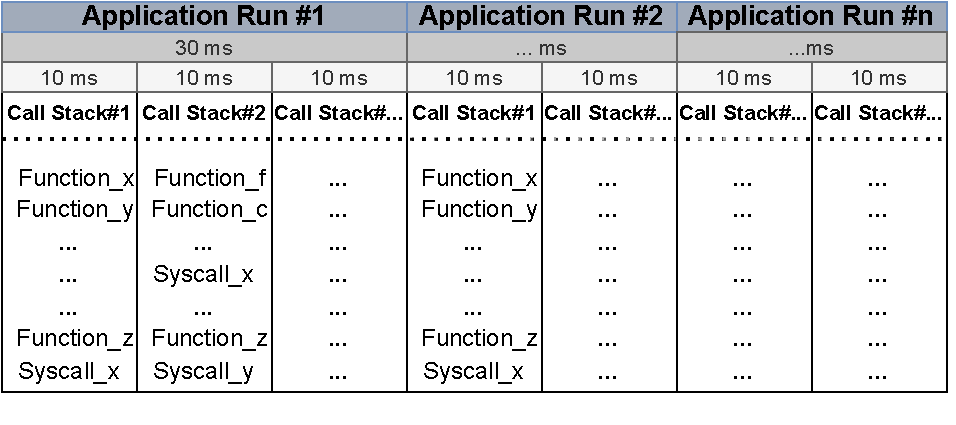
\includegraphics[width=0.8\linewidth]{images/pdfs/callstack_recording.pdf}
    \caption{System-wide call stack recording.}
    \label{fig: Call Stack Recording}
\end{figure*}


\subsubsection{2- Family-group Identification \& Sorting}

A family group, in the context of function and system calls, refers to the hierarchical relationships between parent and child calls. A 'parent' call is a function or system call that invokes another call, while a 'child' call is the one being invoked. Building a family-group linkage for all application function calls and system calls is essential for understanding the execution flow of a program. This involves creating a structured list that maps these relationships, capturing the hierarchy and dependencies within the call stack. By establishing this linkage, we can trace the flow of execution, identify dependencies, and gain insights into how different parts of the application interact. This hierarchical mapping is particularly valuable for debugging, performance analysis, and optimizing system behavior, as it provides a clear and organized view of the call stack structure.

In the context of a snapshot $SP$, denoted as a set of call stacks $SP=\{Call-Stack^i|1\leq i \leq n\}$, each call stack $Call-Stack^i = \langle F^a, F^b, ..., F^d \rangle$ represents a sequence of function calls during the execution. The term "family-group" refers to a collection of related function calls and system calls that exhibit a parent-child relationship. Formally, for a call stack $Call-Stack^1 = \langle F^a, F^b, F^c \rangle$, the family-group is represented as $Family-Group=\{(F^a, F^b), (F^b, F^c)\}$.

To identify family groups, we analyze call stacks individually, counting the frequency of connections between specific parent and child function calls. For example, in Figure \ref{fig: fam}, the link from function call C to D appears only once across all sampled call stacks, indicating a single occurrence in the collected data.

\begin{figure*}[tbp]
    \centering
    \includegraphics[width=0.8\linewidth]{images/pdfs/fam.pdf}
    \caption{An example of Family-group Identification.}
    \label{fig: fam}
\end{figure*}

Once family groups are identified, the next step is to rank them. This involves two sorting functions. First, we sort the groups based on the number of call counts, prioritizing functions that appear most frequently. This ensures that functions with the highest potential to impact system performance are ranked higher, as even a slight increase in their execution time can cause significant degradation. Functions that are rarely called are deprioritized, as they are less likely to affect overall performance.

However, this raises the question: what if a rarely called function is the culprit? To address this, we assume that functions consistently performing poorly have already been identified and handled during the testing phase. This research focuses on the production phase, where tracing is used to gather data on potential issues that were undetected during testing. Tracing provides diagnostic data for problems that cannot be recreated in a controlled environment but cannot solve the issues on its own. Therefore, it is logical to prioritize monitoring functions with the highest system overhead. Algorithm \ref{familygroup} outlines the steps for identifying and ranking family groups based on call counts.

\begin{algorithm}[tbp]

  \caption{Family-group Identification \& Sorting}\label{familygroup}

  \begin{algorithmic}[1]
    % \State $SortedFamilyGroupList=[\phi]$
    \State $FamilyGroupList=[\phi]$
    \State $FamilyGroupCount=[\phi]$
    \State $CallStackSnapshots=[CS_0,CS_1,CS_2,...,CS_N]$

    \ForEach{$Snapshot \in CallStackSnapshots$}
        \State Extract all FamilyGroups from $Snapshot$
        \State E.g., $FunctionCall_{parent}.FunctionCall_{child}$
        \State $FamilyGroup = [FG_1,FG_2,FG_3,...,FG_n]$
        \ForEach{$Family \in FamilyGroup$}
            \If{$Family \notin FamilyGroupList$}
                \State Add $Family$ to $FamilyGroupList$
            \Else
                \State $family_{index}$ = Find index of $Family$ from $FamilyGroupList$
                \State $FamilyGroupCount[family_{index}] \mathrel{+}= 1$
            \EndIf
        \EndFor
    \EndFor
    \State Sort $FamilyGroupList$ based on the values in $FamilyGroupCount$
    \State \Return $FamilyGroupList$
  
  \end{algorithmic}
\end{algorithm}



\subsubsection{3- Coefficient Of Variation (CoV) Ranking}

Once family groups are identified and sorted, we rank the function and system calls within these groups based on their Coefficient of Variation (CoV) in execution time. This prioritizes monitoring of the most volatile or fluctuating calls in the production environment. Calls with a higher standard deviation relative to their mean execution time are considered riskier, as they are more likely to cause performance fluctuations. Algorithm \ref{covranking} outlines the steps for ranking family groups using parent function calls and their CoV values.

\begin{algorithm}[tbp]

  \caption{CoV Ranking of Function Calls}\label{covranking}
  \begin{algorithmic}[1]
    \State Given that each snapshot is 10ms
    \State $FunctionsExecTimeList=[\{MC_1[ET_1,...ET_n]\},...,\newline\{MC_n[ET_1,...,ET_n]\}]$
    % \State $CoVRankedList = CoVRanking(FunctionsExecTimeList)$
    \State $CoVList=[\phi]$
    % \State $RankedFunctionList=[\phi]$
    \ForEach{$MC \in FunctionsExecTimeList$}
        \State $\mu =$ Calculate Mean Of $MC$
        \State $\sigma =$ Calculate Standard Deviation Of $MC$
        \State $CoV_M = \frac{\sigma}{\mu}$
        \State Add $CoV_M$ to $CoVList$
    \EndFor
    \State Sort $FunctionsExecTimeList$ based on the values in $CoVList$
    \State \Return $FunctionsExecTimeList$
    
    
  \end{algorithmic}
\end{algorithm}

\subsubsection{4- Function List Cutoff}\label{cutoffsec}

To effectively monitor the performance of a large application, it is essential to focus on a limited number of functions. The cutoff number should be determined by balancing the cost of monitoring with the desired level of detail. For example, monitoring the top 5\% or the 95th percentile of functions on the list ensures coverage of those most likely to impact system performance. The list is already sorted based on family-group call counts and the Coefficient of Variation (CoV) of function execution times, prioritizing the most performance-critical functions. However, this phase must be repeated regularly to account for changes in the application or operating system, ensuring that newly introduced or deprecated functions are included or excluded as needed.


\subsubsection{Explanation With An Example}
Figure \ref{fig: fam} illustrates the processes involved in the Tracing-Function Selection Phase. Using Perf's record function, we can directly identify the function that initiated a call to the next function. In this example, a sampling rate of 10 milliseconds is used. The figure shows that FunctionA() called FunctionB() in the first call stack, forming a family-group A--B with a count of two, as A called B on two distinct occasions in the sample. Although A and B appear in the first two call stack snapshots, we deduce (based on \cite{han2012performance}) that the second snapshot represents the continuation of the initial call from A.

Next, we sort all family-groups by their count in descending order, ensuring the most impactful groups are ranked highest. To estimate the execution time of FunctionA(), we observe that it appears in the first two call stacks but not the third, suggesting an execution time of 20 milliseconds (10ms + 10ms) for the first call. After calculating execution times for all functions, we compute their Coefficient of Variation (CoV) values to rank them based on their variability. Finally, we determine a cutoff by retaining only the top two family-groups, $\{(X,Y),(Y,Z)\}$. The functions in these groups, $\{X,Y,Z\}$, are then monitored by the proposed approach.

It is important to note that while the identified function calls may correlate with bugs or performance issues, they are not necessarily the root cause. At this stage, we focus on identifying the most fluctuating and latency-contributing functions, marking them as candidates for runtime monitoring. Our goal is not to detect performance issues at this stage or during runtime. Instead, we assume the program has already undergone functional and non-functional testing, with any bugs identified and resolved. Our objective is to select sufficient candidates for runtime monitoring to detect significant behavioral changes, which can then inform further trace configuration adjustments.


\subsection{Phase \#2: Change Detection}

In the change detection phase, we employ Autoregressive Integrated Moving Average (ARIMA) models \cite{ho1998use} for each function and system call in the cutoff sorted list. Each model is supplied with time-series data representing the execution times of these functions and system calls. The ARIMA models predict the expected value at time $T$ based on data up to time $T_{-1}$. If the actual reading at time $T$ significantly deviates from the predicted value—exceeding a predefined threshold determined by the system's sensitivity—the $isAnomaly$ flag for the $anomalyScore$ function is set to true; otherwise, it is set to false. A substantial mismatch between the actual and predicted readings indicates a disruption in the previous trend. If this deviation exceeds the acceptable threshold, we infer that the function or system call may be problematic.


Figure \ref{fig: Change Detection Phase} shows the flow diagram for the change detection phase. The $anomalyScore$ function determines the anomaly score, with a higher score corresponding to a higher frequency of abnormalities or a lower score for less frequent abnormalities. A threshold is established, and if the $anomalyScore$ surpasses this threshold, tracing is enabled for the suspected function or system call. Conversely, as the system returns to a new normal state and ARIMA predicts along these new levels, the $anomalyScore$ decreases. Once it falls below the threshold, tracing for those functions is disabled, assuming that the recorded changes have been adequately captured, and further logging would be unnecessary. Algorithm \ref{changedetect} outlines the steps of the change detection phase, encapsulating the proposed adaptive tracing approach.

\begin{figure}[tbp]
    \centering
    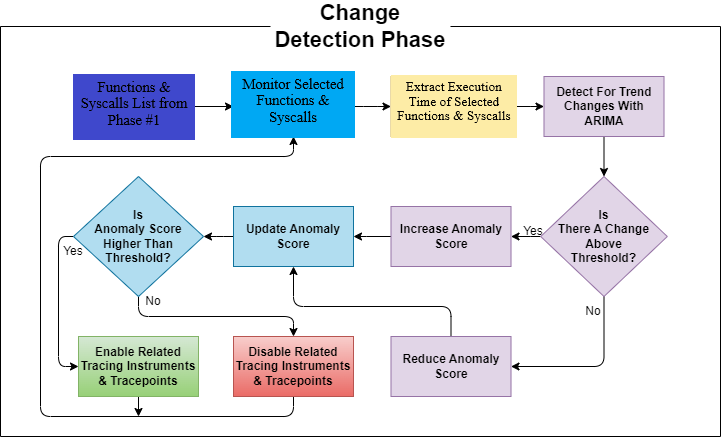
\includegraphics[width=\linewidth]{images/change_detection.png}
    \caption{Change Detection Phase}
    \label{fig: Change Detection Phase}
\end{figure}


\begin{algorithm}[tbp]

  \caption{Change Detection Algorithm}\label{changedetect}

  \begin{algorithmic}[1]

    \State $anomalyScore=[M_1, M_2, M_3,...M_n]$
    \Function{Anomaly\_Score}{$FunctionID$,$isAnomaly$,$\beta$}
        \State $anomalyScore[FunctionID]=(\beta \times isAnomaly)+((1 - \beta) \times anomalyScore[FunctionID])$
    \EndFunction
    
    \Function{Predict\_T}{$FunctionExecData$}
        \State $T_p$ = ARIMA($FunctionExecData$)
        \State \Return $T_p$
    \EndFunction
    
    \Function{Change\_Detection}{$FunctionExecutionTimeDataset$,\newline$Threshold_{arima}$,$\beta$,$Threshold_{anomaly}$}
        \State $FunctionExecData=FunctionExecutionTimeDataset[1:]$
        \State $T_{actual} = FunctionExecutionTimeDataset[0]$
        \State $T_{predict} = Predict\_T(FunctionExecData)$
        \State $\Delta_{Diff} = |T_{actual} - T_{predict}|$
        \State $isAnomaly=False$
        \If{$\Delta_{Diff} > Threshold_{arima}$}
            \State $isAnomaly=True$
        \Else
            \State $isAnomaly=False$
        \EndIf
        \State $Anomaly\_Score(FunctionID, isAnomaly,\beta)$
        \If{$anomalyScore[FunctionID] >= Threshold_{anomaly}$}
            \State \Return Anomalous
        \Else
            \State \Return Normal
        \EndIf
    \EndFunction

    \State $FunctionExecutionTimeDataset=[\{T,...,T_{-n}\},...,\{...\}]$
    \State $Threshold_{arima}=X$, $Threshold_{anomaly}=Y$, $\beta=Z$
    \ForEach{$FunctionExecData \in FunctionExecutionTimeDataset$}
        \If{$Change\_Detection(FunctionExecData,Threshold_{arima},\newline\beta,Threshold_{anomaly}) \neq Normal$}
            \State Enable tracepoint(s) relevant to the problematic function.
        \Else
            \State Disable tracepoint(s) relevant to the function.
        \EndIf
    \EndFor
        
  \end{algorithmic}
\end{algorithm}

In the Change Detection phase, we rely on two fundamental components: the ARIMA model and the $anomalyScore$ function. The following subsections provide a detailed examination of each of these components. 

\subsubsection{Autoregressive Integrated Moving Average (ARIMA)}\label{methodology: autoregressive integrated moving average (arima)}

Autoregressive Integrated Moving Average (ARIMA) is an algorithm that predicts future data values based on trends from past time-series data \cite{ho1998use}. Widely used in financial markets, ARIMA leverages time-series data and statistical analysis to understand datasets and forecast future trends~\cite{qiu2019short}. It predicts future values based on prior data, making it suitable for applications such as estimating a company's earnings or forecasting stock prices using historical performance and trends.

ARIMA combines the features of autoregressive (AR) and moving average (MA) models. An AR(1) autoregressive mechanism predicts the current value based on the immediately preceding value, while an AR(2) mechanism uses the two previous values. Moving averages smooth out anomalies by calculating averages of subsets of the dataset. By integrating these techniques, ARIMA models can predict trends, phases, periodicity, and other non-static patterns in data~\cite{qiu2019short}.

\subsubsection*{Why ARIMA?}
We selected ARIMA over other methods for two key reasons. First, ARIMA predicts future values based on past trends in data, allowing us to detect when a trend is broken. This is indicated by significant deviations between predicted and actual metric readings beyond an acceptable threshold. Second, ARIMA identifies all trend changes, whether caused by anomalies, attacks, or shifts in system/application workload or behavior. In such cases, additional tracing data is required to determine the root cause of the unexpected change.

Unlike machine learning or deep learning approaches, ARIMA does not adapt to new changes but instead relies on past trends for predictions. This ensures the method does not learn from recent fluctuations, preserving its ability to detect genuine changes in trends. While reinforcement learning could have been a viable alternative, as discussed in the literature review, it is impractical to implement in this context. Reinforcement learning requires a well-defined reward function, which is not feasible here because tracing provides hypotheses—not definitive facts—and requires expert analysis of trace logs to perform root cause analysis.
% The reason for selecting ARIMA over other methods is that we utilized the property of ARIMA, which makes future predictions based on past trends in data. By leveraging this property, we could identify when a past trend has been broken, given that the predicted metric readings are wildly off from the actual metric readings beyond an acceptable threshold. Another reason is that ARIMA would predict all trend changes, regardless of whether they are caused by an anomaly, an attack, or simply a change in the workload or behavior of the system/application. In these cases, it would be necessary to collect additional tracing data to understand why the unexpected change occurred. Unlike machine learning or deep learning approaches, we relied on the fact that the algorithm we will be using should not learn based on new changes but rather predict based on the past trends it used to maintain. This is so that the method does not learn about patterns of recent fluctuations; otherwise, it breaks the whole purpose of change detection in trends. Reinforcement learning could have been a good approach, as discussed in the literature review, given that we were directly solving the problem. However, it is impossible to implement reinforcement learning because it is not practical to develop a reward function for something where the outputs are hypotheses and not definite facts. Meaning tracing will provide us with only trace data which is not any concrete fact as to if it has detected the problem correctly unless an expert uses those trace logs to perform root cause analysis to find out.

% It is possible for ARIMA models to include moving average terms, differencing operations, and autoregressive terms. There are several abbreviations used:

% \begin{itemize}
%   \item It may be described as an MA model if it only involves moving average terms.
%   \item A model with only autoregressive terms is called an AR model. 
%   \item A model may be called ARMA in cases where there is no differencing.
% \end{itemize}

Depending on the use of the model, we need to decide the order of the model's elements (AR order, differencing order, MA order). For example, an ARIMA with two AR terms would be (2,0,0), MA(2) models are defined as ARIMAs of order (0,0,2), and the order of an AR model with first-order difference and a moving average term would be (1,1,1).

\subsubsection*{ARIMA(1,0,1)}\label{methodology: arima(1,0,1)}

The ARIMA(1,0,1) model consists of an autoregressive process AR(1) and a moving average process MA(1) of the first order. There are three parameters in the forecast model: a moving average factor $\theta$, an autoregressive factor $\varphi$, and a constant term $c$.


\[ \hat{x}_{t+1} = c + \varphi x_t + \theta\varepsilon_t, \hspace{1cm} \varepsilon_t = x_t-\hat{x}_t\]


\subsubsection*{ARIMA(1,1,1)}\label{methodology: arima(1,1,1)}


The ARIMA(1,1,1) model is a version of the ARIMA(1,0,1) model that is integrated. We use first-order differences instead of past values to build the autoregressive model.

\[ \hat{x}_{t+1} = x_t + \varphi\Delta x_t + \theta\varepsilon_t, \hspace{1cm} \varepsilon_t = x_t-\hat{x}_t\]

To account for linear trends in the data, we propose using the ARIMA(1,1,1) model. If the change in trend is non-linear, we assume it indicates a problematic shift in the metric's behavior. For example, if a web server that typically maintains 10\% CPU usage suddenly spikes to 30\% and then 90\%, this quadratic change in the trend is considered a performance issue. Using a higher-order ARIMA model would risk closely predicting such non-linear trends, defeating the purpose of detecting anomalies. However, for gradual changes—such as an organic increase in a web server's popularity—the ARIMA(1,1,1) model can automatically adjust to predict along the new trendline. This justifies our choice of a first-order ARIMA(1,1,1) model.


\subsubsection{Anomaly Score}

For our approach to the adaptive tracing problem and to address $RQ4$, it is essential to know the following:

\begin{itemize}
  \item When to alert or take action?
  \item For how long to keep the alert or action intact?
  \item When to stop the alert or revert the action?
\end{itemize}

Here we have an example of a response time graph in Figure. \ref{fig:response time}. This figure has five markers that show a change happening in the graph. Now, we may ask: 

\begin{itemize}
  \item \verb|(a)|Do we take action or send an alert at 1, which shows the first jump in response time?
  \item \verb|(b)|Do we set off an alert/action at 2 when we observe some consecutive drops in response time? 
  \item \verb|(c)|Do we take action or alert at 3 when the response time has created a new high?
  \item \verb|(d)|Given that we had taken action or set off an alert at 1, 2, or 3, till when do we keep the action or alert active?
  \item \verb|(e)|How should we recalibrate our normal range parameters when we observe a shift in the readings?
\end{itemize}

\begin{figure}[tbp]
    \centering
    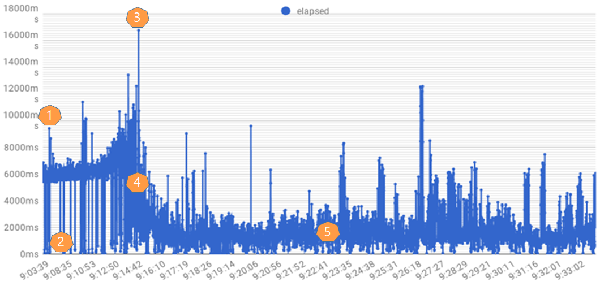
\includegraphics[width=\linewidth]{images/fig_rs.png}
    \caption{A response time graph}
    \label{fig:response time}
\end{figure}

We know that both setting off an alert for human intervention and taking an automatic action is both very costly \cite{beyer-2016} \cite{ewaschuk-no-date} \cite{parker-2020}. So, to answer questions (a), (b), and (c), we have to look into how these changes take place. At 1, although it is the first abnormal reading to the upside, it makes no sense to take action or set off an alert. The justification for this decision is that it is the very first abnormal reading, and it is possible that this could have been just a one-time spike that would never be seen again, or it is in such a minor frequency of occurrence that it is not worth it to page someone for this. It also makes no sense to keep tracking or deploying resources such as tracing for components where we might have read just one single anomaly reading. It is possible that it could have been a one-time, isolated incident, and we are never to see such an anomaly again. This brings us to the importance of frequency of occurrence. At 3, we can already see there have been quite several spikes, so it suggests that there is a high frequency of reoccurring abnormalities going on. Therefore, it makes sense to take action or set off an alert at 3.

However, to answer (d), we must have sound logic behind our actions. Once we have set off the alert at 3, it can be observed that the response time goes back down with a significant change at 4. Although, at 4 we can see the major retrace, just like we cannot set off an alert right away when we see the first occurrence of abnormalities; similarly, we cannot retrace our alert on the first change back towards the normal range. This is because we have yet to confirm if the change back was only a temporary retrace or if it is a much more permanent one. To get that confidence of confirmation, we would have to wait for more readings in the normal zone. That is why it makes much more logical sense to turn off the alert at 5 because at 5 we have a much more established reading.

To solve this problem, we have employed a function named the anomaly score. The anomaly score, inspired by previous work in \cite{ehlers2011self}, aims to track the significance of anomalous readings obtained from execution time data. It operates by assigning a score to a function call's execution time based on the frequency of anomalous readings. The anomaly score increases as the frequency of anomalous readings increases and decreases as the frequency of anomalous readings decreases. Here we define anomalous reading as execution time which deviated from ARIMA's prediction beyond the defined threshold.

The anomaly score function is defined as:

\begin{equation}
anomalyScore = (\beta \times isAnomaly) + ((1 - \beta) \times anomalyScore)
\end{equation}

Where:

\begin{itemize}
  \item $\beta$ is a decaying factor that controls the rate of rise or fall of the anomaly score and should be set based on the system's sensitive nature to performance impacts or the tasks it performs. A higher $\beta$ value results in a faster reaction to an anomaly, and vice versa.
  \item $isAnomaly$ is a boolean flag that is either 0 or 1, representing if the reading was anomalous or not.
\end{itemize}

The $isAnomaly$ flag is calculated based on the difference in distance between the actual reading of a metric value and the ARIMA predicted value for the same metric. If the distance exceeds the defined threshold, the metric is considered anomalous, and the anomaly flag is triggered.




\subsubsection{$RQ2$: How can we detect behavior changes on runtime?}
To address $RQ2$, we assume that a healthy and stable system—one that has not undergone any system-level or application-level updates or changes—should maintain consistent trends in its system and application-level metric data. This assumption is based on the rationale that while specific tasks may cause fluctuations in metric data, the underlying trend should remain stable. For example, if executing a function call takes 1 second, executing 10 of the same function calls should ideally take 10 seconds (assuming no parallel processing). However, if we observe a sudden change—such as a single function call taking 1.5 seconds, then 2 seconds, and so on—this indicates a deviation from the expected trend. Such changes may result from increased load elsewhere in the system, but they warrant investigation as they impact the optimal performance of the application. Figure \ref{fig: Change Detection In Trend - 1} illustrates a scenario of a sudden upward trend that requires tracing.

\begin{figure}[tbp]
    \centering
    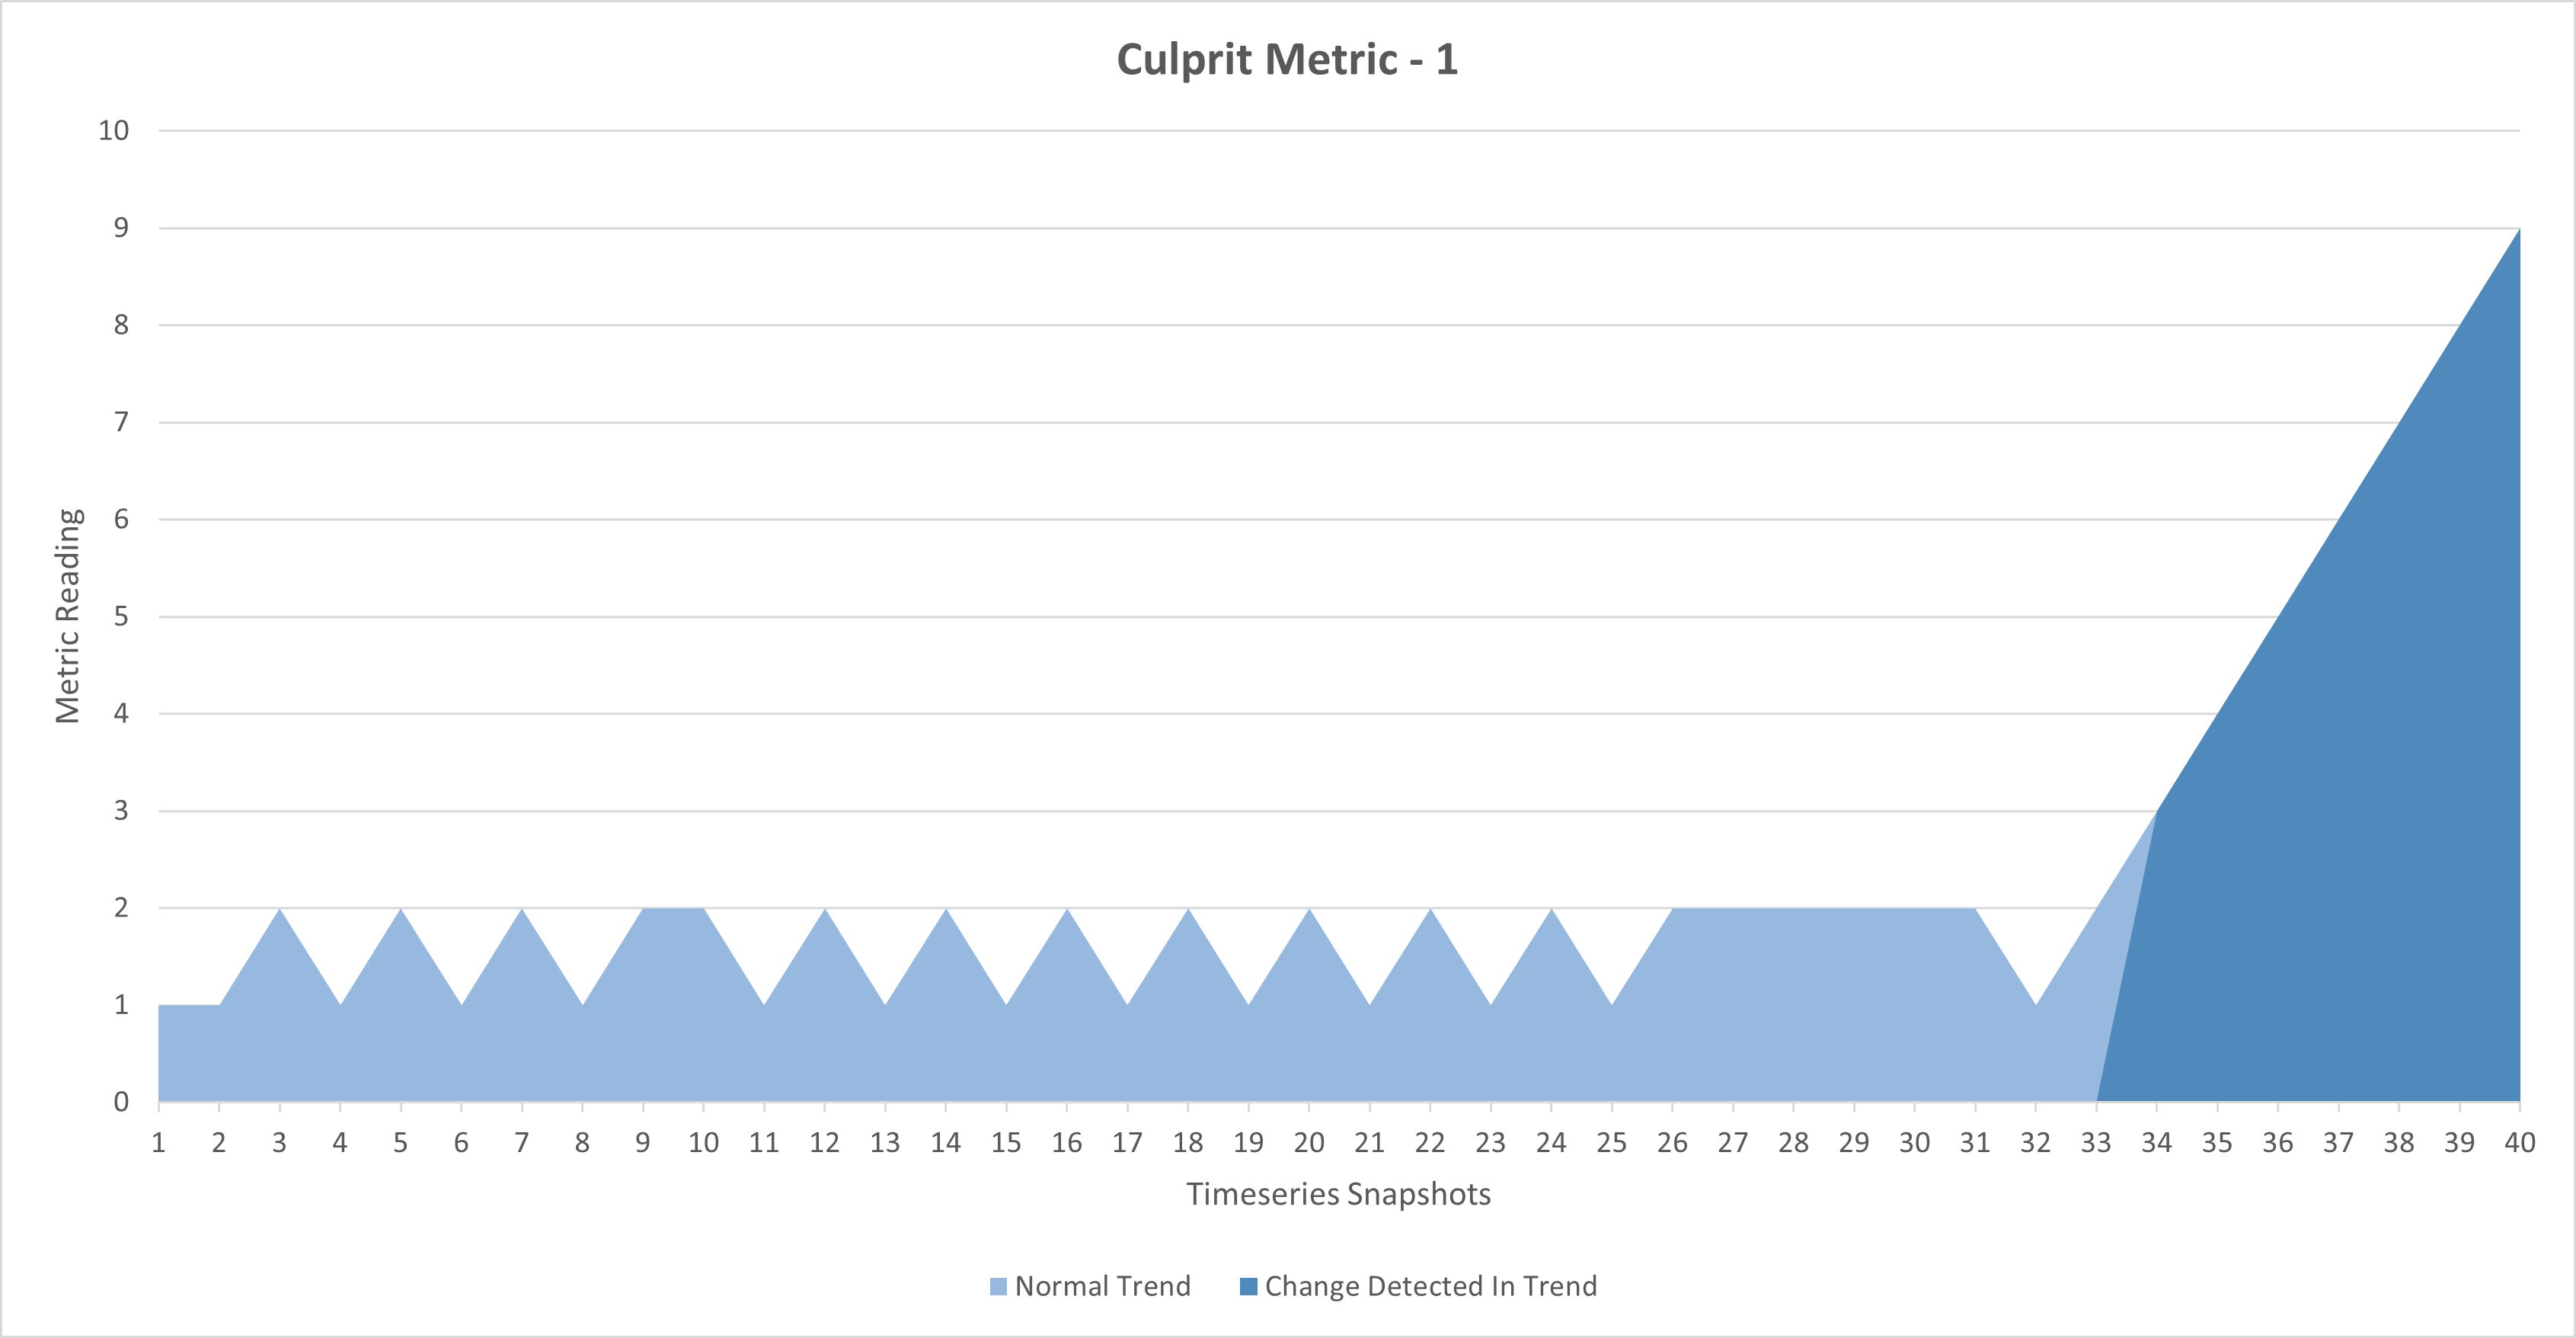
\includegraphics[width=\linewidth]{images/culprit_metric1.png}
    \caption{A sudden upward trend that needs to be traced.}
    \label{fig: Change Detection In Trend - 1}
\end{figure}

Another reason for focusing on change detection, rather than relying on general thresholds or expected value ranges, arises in scenarios like deadlocks. For instance, if a server application typically maintains 10-15\% CPU usage, a drop below 10\% might suggest improved optimization and better performance. However, it could also indicate a deadlock, where the CPU utilization is constrained because threads are stuck waiting. This ambiguity highlights the importance of monitoring and flagging changes in trends, not just changes in the data itself. Figure \ref{fig: Change Detection In Trend - 2} illustrates the areas requiring monitoring when a trend shifts downward.

\begin{figure}[tbp]
    \centering
    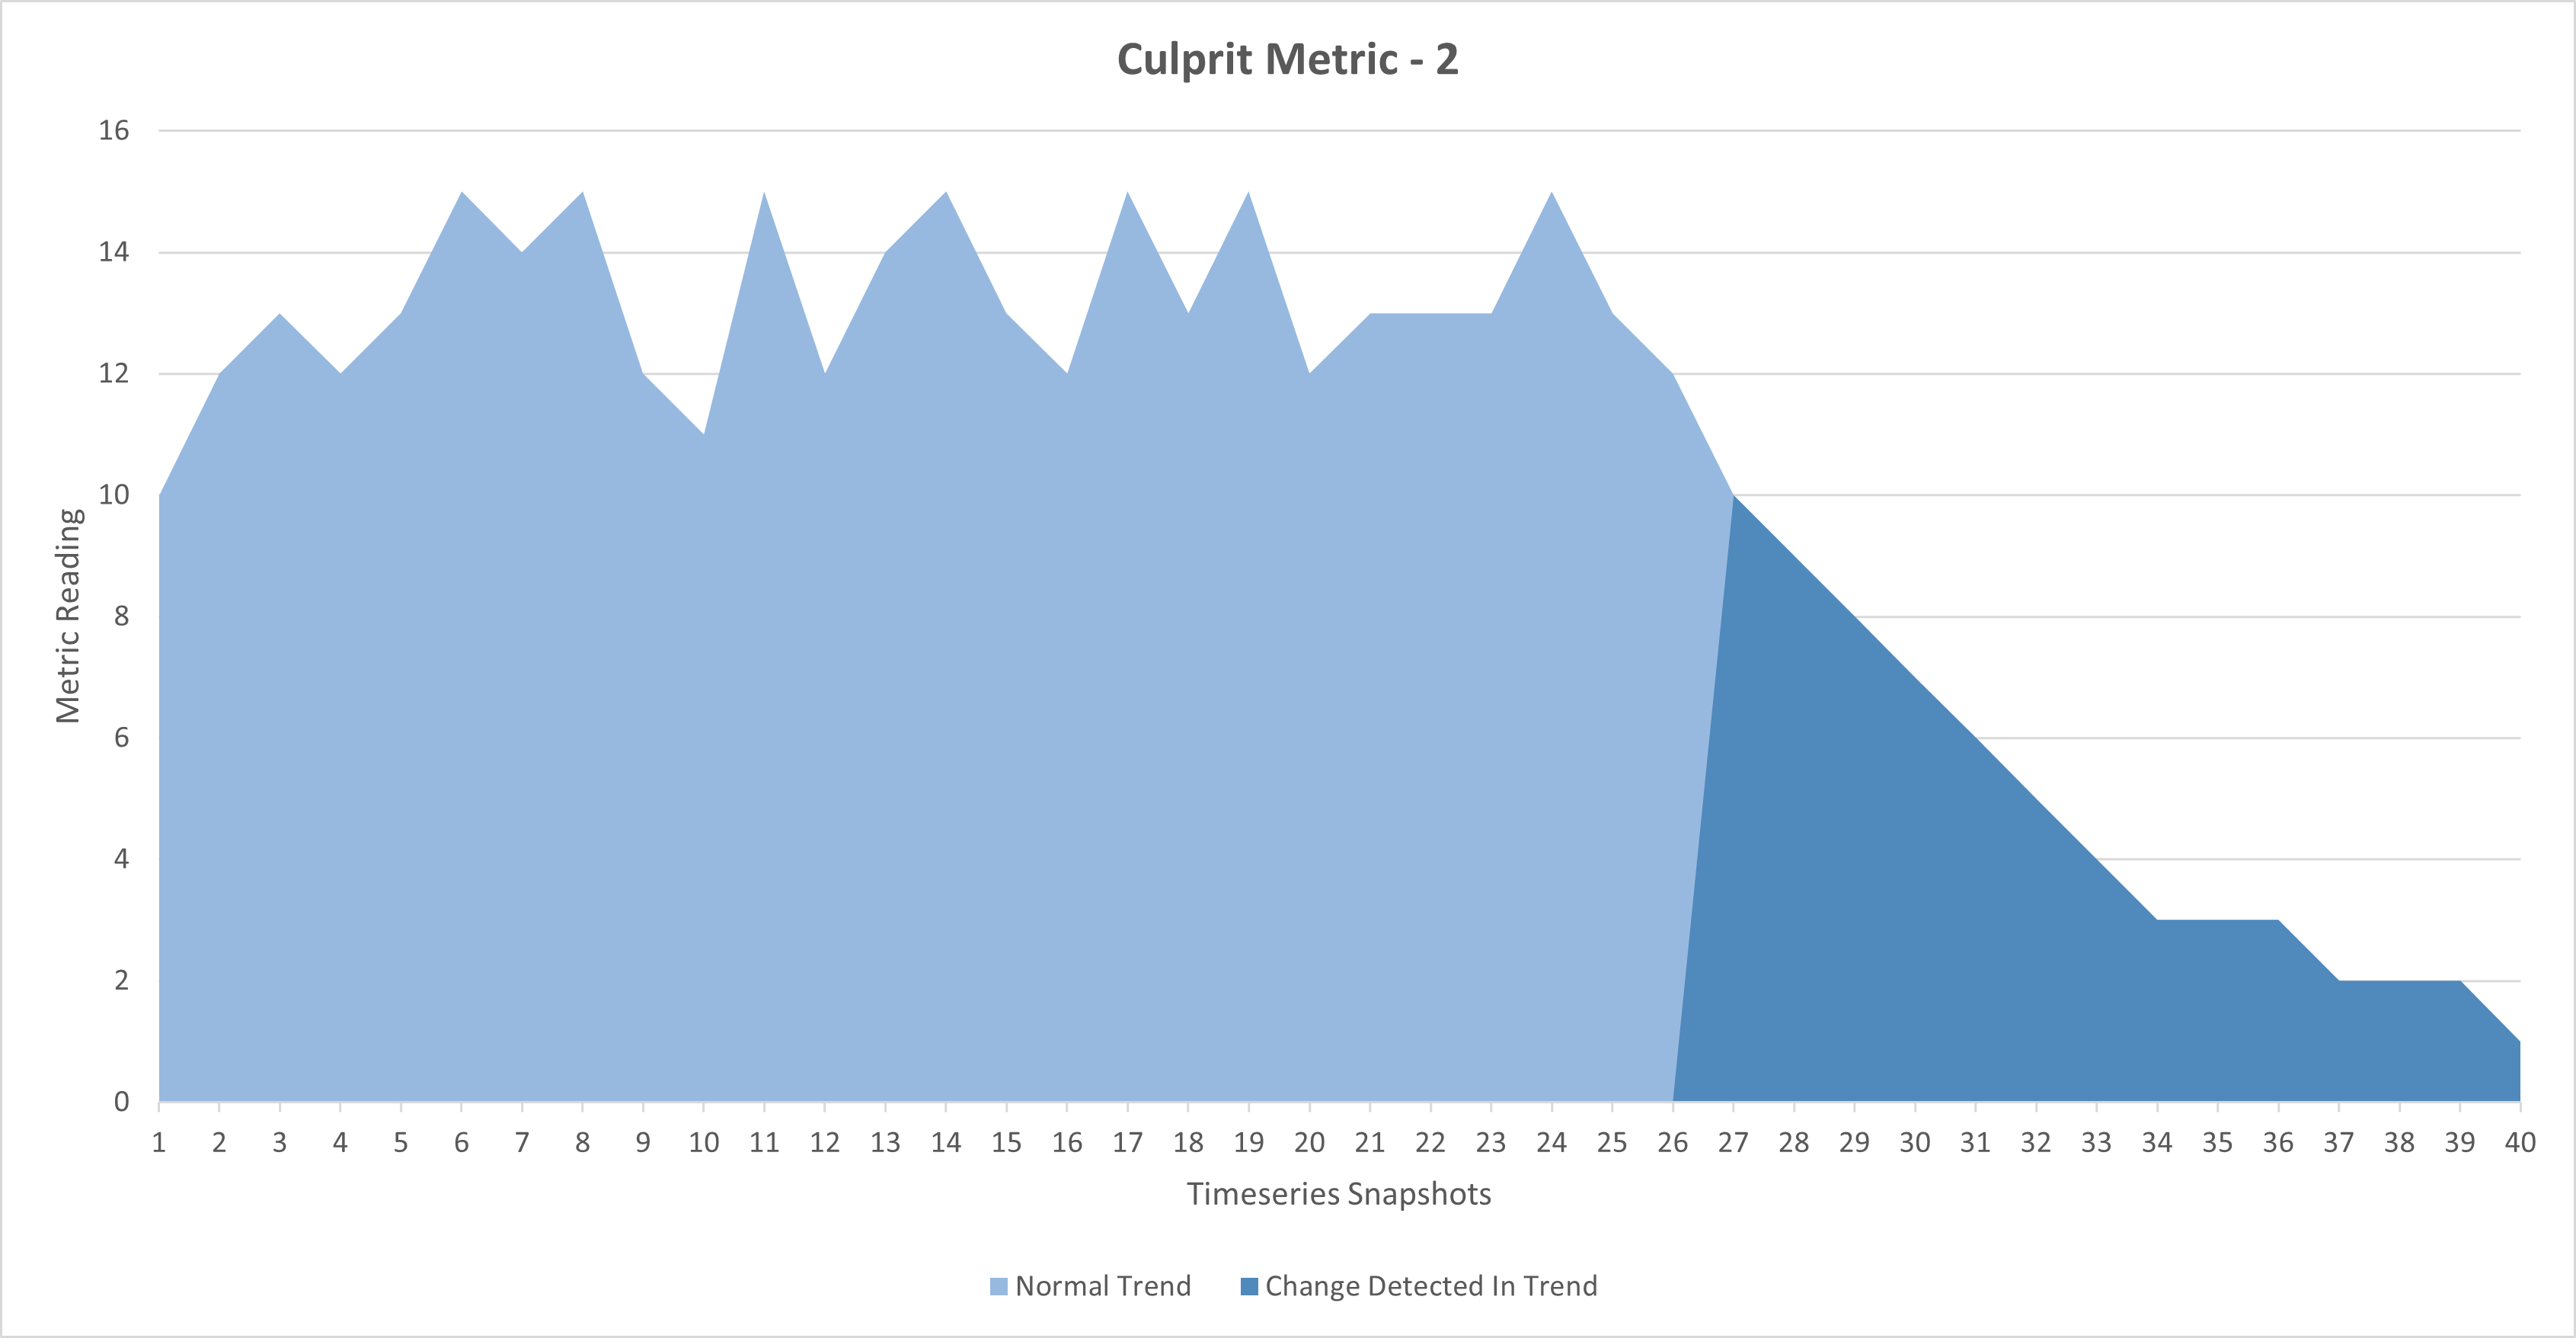
\includegraphics[width=\linewidth]{images/culprit_metric2.png}
    \caption{The areas requiring monitoring when a trend changes to the downside.}
    \label{fig: Change Detection In Trend - 2}
\end{figure}



\subsection{Phase \#3: Trace Configuration Change}

The goal of this phase is to adjust tracing configurations to collect sufficient data for the early detection of potential performance issues. The proposed multi-level adaptive tracing approach enables modifications to tracing configurations at both the application and system levels. When the change detection phase identifies a trend deviation, tracing is initiated for the associated family-groups of the impacted functions, up to a pre-set depth limit (e.g., 20 family members).

To dynamically adjust tracing configurations based on detected changes, a decision mechanism has been implemented. This mechanism relies on two factors: (1) change detection through ARIMA models and (2) a pre-determined acceptable threshold for deviations from the original trend. This decision mechanism addresses \verb|RQ3| by ensuring that tracing configurations are adjusted in response to significant changes, enabling proactive performance monitoring.

System-level tracing is achieved by controlling tracing components that record system-level events and system calls. Similar to the application-level approach, a list of system calls made during various loads and stress phases is compiled, sorted, and ranked. The execution time for each system call is monitored, and if abnormalities or trend changes are detected, a Linux system call table (e.g., \cite{valsorda-no-date}) is used to map the system call to the corresponding kernel-level component. For example, the system call \texttt{sendmsg} is handled by the kernel component \texttt{net/socket.c}, which pertains to the network subsystem. By identifying the relevant kernel-level component, tracing instruments can be enabled to record events related to that component, such as network-related events in this case.

At the application level, tracing is adjusted based on the family-groups identified during the pre-testing phase. When a trend deviation is detected, tracing is initiated for the impacted functions and their associated family-groups, ensuring that sufficient data is collected for analysis.

The proposed multi-level adaptive tracing mechanism adaptively handles both system and application-level tracing, offering a comprehensive approach to performance monitoring and optimization. By adjusting tracing configurations, this phase aims to collect sufficient data for early detection of potential performance issues, helping developers and system administrators identify problems related to configuration, resource failures, resource contention, and internal code bugs.


\section{Evaluation \& Discussion} \label{results}
This section evaluates our proposed approach through real-world examples, demonstrating its effectiveness in adaptive tracing, change detection, and multi-level tracing. The use cases include detecting trend changes in system-level metrics to reduce tracing overhead (Use Case 1), identifying hardware driver and application communication issues (Use Case 2), pinpointing performance-degrading function calls or classes (Use Case 3), and monitoring system-call execution times to adaptively configure system-level tracing (Use Case 4).

\textbf{Scope of these case studies.} The four case studies presented here are \emph{illustrative demonstrations} of the adaptive tracing framework rather than prospective blind evaluations. In each case, a known Bugzilla performance bug report is used to confirm whether the framework correctly flags the responsible function or kernel component from the ranked candidate list. The primary claim is not that the framework independently discovered a previously unknown fault, but rather that (i)~it correctly narrows a large candidate space to a tractable monitored set, (ii)~the anomaly-score mechanism triggers and releases tracing at the expected times, and (iii)~the implicated function or component aligns with the ground truth in the corresponding bug report. Rigorous prospective evaluation is identified as important future work.

\subsection{Use Case \#1}\label{case studies & evaluation: case study 1}
This case study demonstrates how our proposed adaptive tracing approach detects trend changes in system-level metrics. By detecting these changes, our approach enables selective tracing of relevant components, determines the optimal time snapshots for initiating tracing, and decides how long to trace, thereby reducing overhead and improving efficiency.




\subsubsection{Data Collection}\label{case studies & evaluation: data collection & generation}

We created a PHP script served by an Apache server that randomly loads a large plain text file and echoes it back. The script was designed to trigger this operation with a 30\% probability, alongside random prime number generation to impose CPU load. Over time, the number of concurrent requests was increased five times, starting from 2 and incrementing by 2 each time.

We recorded 35 system-level metrics, as shown in Table~\ref{nmonmetricstable}, using nmon, a Linux performance monitoring tool available under the GNU General Public License~\cite{nmon}. These metrics are grouped into four major categories: (i) CPU, (ii) Memory, (iii) Disk, and (iv) Network.

Snapshot data was recorded every 1 second by setting the ss parameter of nmon to 1. The following command was used:
\[ nmon -f -s 1 -c 3600 \]
Here, the $f$ parameter directs nmon to save the data in the current directory instead of displaying it in the terminal. The process was run for 1 hour. The recorded time-series data was then fed into ARIMA models.

Some key parameters to note include a \texttt{threshold\textsubscript{arima}} of 3\% for both upward and downward deviations. If the difference between the predicted and actual values exceeds 3\%, the reading is flagged as an anomaly. For the \texttt{anomalyScore} function, we set $\beta=0.3$ and \texttt{threshold\textsubscript{anomaly}} = 0.3 for this experiment. Our findings indicate that a $\beta$ value lower than 0.3 introduces significant decision-making lag. Conversely, a $\beta$ value higher than 0.3 causes the anomaly score to rise sharply, crossing the threshold too quickly even for low-frequency anomalies. This occurs because the anomaly score accumulates rapidly with each occurrence, leading to overly sensitive detection.

\begin{table}[tbp]

\centering
\resizebox{\columnwidth}{!}{%
\begin{tabular}{ |l|l|l| }
\hline
\textbf{Category} & \textbf{Metrics} & \textbf{Description} \\
\hline
\multirow{7}{*}{CPU} & CPU\_User\% & CPU time in user mode.\\
 & CPU\_Sys\% &  CPU time in kernel mode. \\
 & CPU\_Wait\% & CPU time waited for I/O. \\
 & CPU\_Idle\% & CPU time were idle.\\ 
 & PROC\_Runnable &  Runnable processes in the run queue. \\
 & PROC\_pswitch & Number of process context switches. \\
 & PROC\_fork & Number of fork system calls. \\  \hline
\multirow{14}{*}{Memory} & MEM\_memfree & Total free RAM. \\
 & MEM\_memshared &  Memory cache across applications. \\
 & MEM\_cached  & In-memory cache for files. \\
 & MEM\_active & Memory used by processes. \\
 & MEM\_buffers & Temporary storage used for disk blocks. \\
 & MEM\_inactive & Pages accessed recently. \\
 & VM\_nr\_dirty & Pages waiting to be written. \\
 & VM\_nr\_mapped & Number of memory mapped pages. \\
 & VM\_nr\_slab\_reclaimable & Pages from the kernel slab memory. \\
 & VM\_pgpgin & Number of pages brought in from disk. \\
 & VM\_pgpgout & Number of pages written out to disk. \\
 & VM\_pgfree & Number of pages free since the last boot. \\
 & VM\_pgactivate & Number of page activations since the last boot. \\
 & VM\_pgfault & Minor faults since the last boot. \\ 
 & DISKBSIZE\_sda & Number of disk blocks are read and written.\\ 
 & NET\_enp0s3-read-KB/s & Data in KB is received on the interface.\\
 & NET\_enp0s3-write-KB/s & Data in KB is sent on the interface. \\
\hline
\end{tabular}%
}
\caption{Selected Nmon Metrics.}
\label{nmonmetricstable}
\end{table}



\subsubsection{Change Detection With ARIMA}\label{case studies & evaluation: change detection with arima}

Figure \ref{fig: c1_s1_0} shows the cumulative number of metrics flagged and unflagged by our proposed approach at any given time, while Figure \ref{fig: c1_s1_00} provides a categorized cumulative view of the same data. From Figure \ref{fig: c1_s1_00}, we observe five prominent humps in CPU-related metrics initially. Over time, these humps flattened out, demonstrating that our proposed approach can adapt to a system's new normal. As we increased the number of concurrent requests fivefold, CPU utilization also rose. However, once the increases stabilized, ARIMA adjusted its predictions for CPU-related metrics to align with the new trend. This reduced the discrepancies between ARIMA's predictions and actual readings, resulting in fewer CPU-related metrics being flagged as the system adapted to its new normal.

\begin{figure}[tbp]
    \centering
    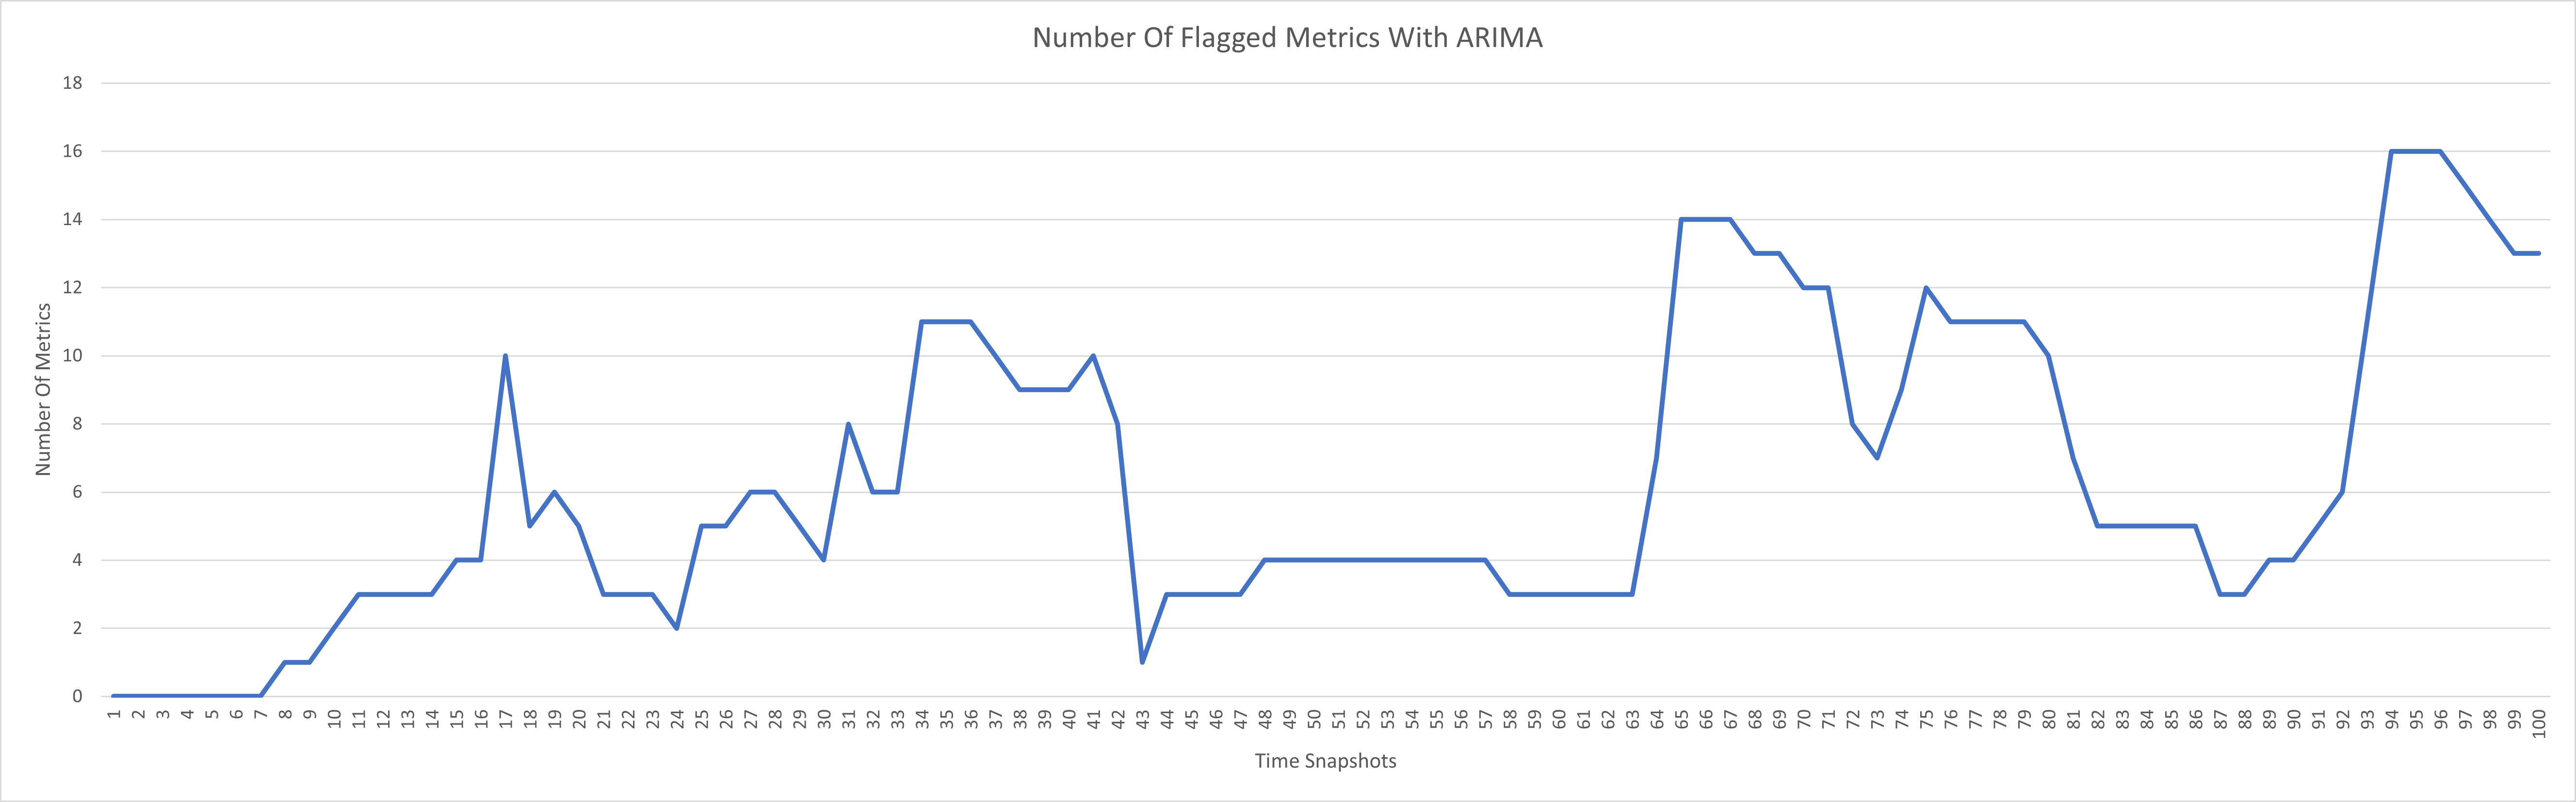
\includegraphics[width=\linewidth]{images/metrics_charts/30_pct_file_load/c1_s1/0.png}
    \caption{ARIMA Flagged Metrics Cumulative Summary | Case Study: 1}
    \label{fig: c1_s1_0}
\end{figure}


\begin{figure}[tbp]
    \centering
    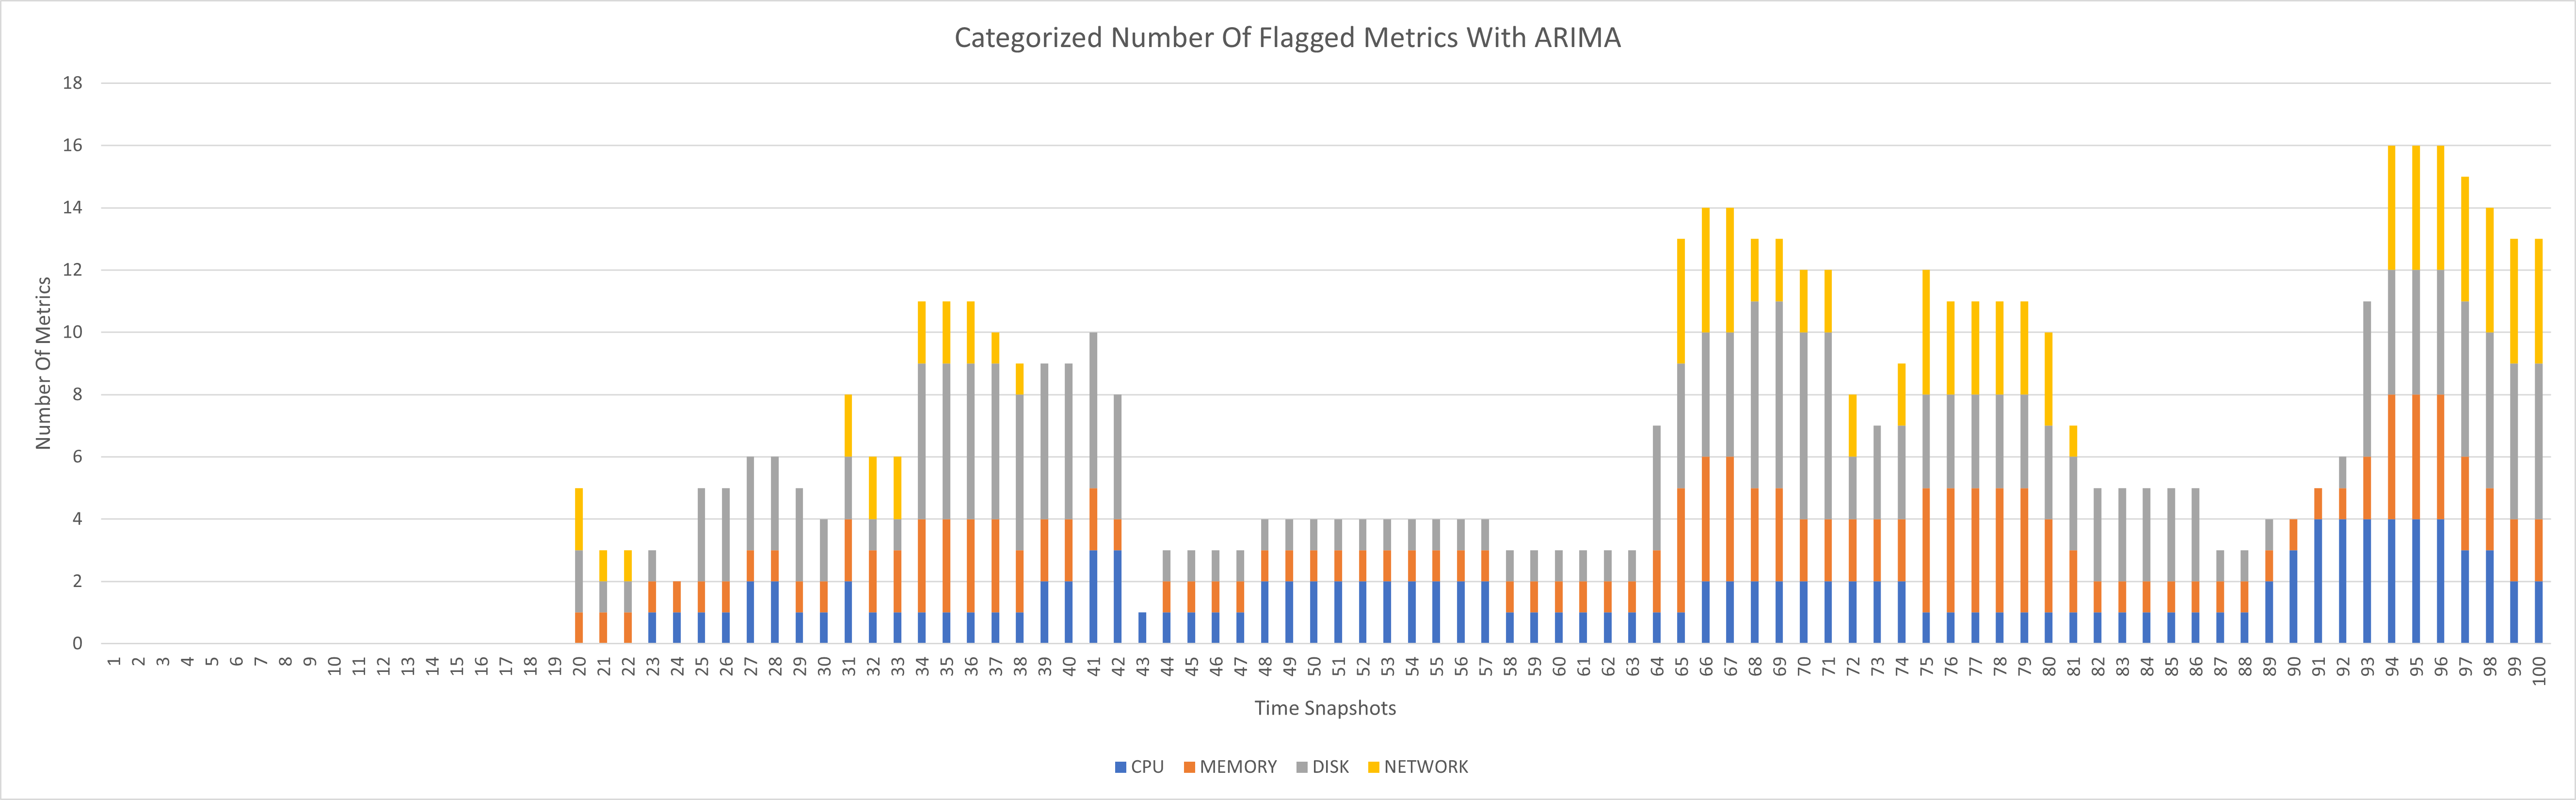
\includegraphics[width=\linewidth]{images/metrics_charts/30_pct_file_load/c1_s1/00.png}
    \caption{ARIMA Flagged Metrics Categorized Summary | Case Study: 1}
    \label{fig: c1_s1_00}
\end{figure}

The total of 21 metrics were flagged by ARIMA, as shown in Table \ref{arimaflagc1s1}. It is important to note that not all metrics were flagged simultaneously or remained flagged for the same duration. To understand how each metric was handled, we analyzed their individual data in detail.



Figure \ref{fig:c1_s1_cpu} shows the CPU-related metrics that were recorded during the experiment. $ARIMA Flagged$ represents the timestamps where the $threshold_{arima}$ was triggered, and $ARIMA Take Action$ areas to represent where it was suggested to enable tracing for the metric's related component(s). Most of the ARIMA prediction figures show a lag. However, the figures with the least number of ARIMA flags (i.e., detected as an anomaly) have the shortest lag. The reason for this is that ARIMA predicts along a past trend. If the trend is not broken, then predicting along the trend will not result in a lag compared to the actual reading.

\begin{table}[tbp]
\centering
\begin{tabular}{ |l|l| }
\hline
\textbf{Category} & \textbf{Flagged Metrics} \\
\hline
\multirow{5}{*}{CPU}
 & CPU\_User\% \\
 & CPU\_Sys\% \\
 & CPU\_Idle\% \\ 
 & PROC\_Runnable \\
 & PROC\_pswitch \\ \hline
\multirow{4}{*}{Memory}
 & VM\_nr\_dirty \\
 & VM\_pgpgout \\
 & VM\_pgfree \\
 & VM\_pgfault \\ \hline
\multirow{8}{*}{Disk}
 & DISKBSIZE\_sda \\
 & DISKBSIZE\_sda5 \\
 & DISKBUSY\_sda \\
 & DISKBUSY\_sda5 \\
 & DISKWRITE\_sda \\
 & DISKWRITE\_sda5 \\
 & DISKXFER\_sda \\
 & DISKXFER\_sda5 \\ \hline
\multirow{4}{*}{Network}
 & NET\_enp0s3-read-KB/s \\
 & NET\_enp0s3-write-KB/s \\
 & NETPACKET\_enp0s3-read/s \\
 & NETPACKET\_enp0s3-write/s \\
\hline
\end{tabular}
\caption{ARIMA Flagged Metrics | Case Study: 1}
\label{arimaflagc1s1}
\end{table}

Figure \ref{fig:c1_s1_02} shows that for CPU\_User\%, there have been four zones where it was advised to enable relevant tracing elements. We can also see that most of the major changes were correctly detected. Similar results were observed in Figure \ref{fig:c1_s1_04} for CPU\_Sys\%. If we look into the setup of data generation, then the advised areas make sense because we had gradually increased concurrent requests five times. For CPU\_Idle\%, we can see in Figure \ref{fig:c1_s1_06} that it was advised to trace related components for a small portion of time. While we check the same time snapshot area on CPU\_User\%, it shows a drastic spike.
On the other hand, for PROC\_Runnable, we observe three areas where it was flagged in Figure \ref{fig:c1_s1_08}. This aligns with the 30\% probability of loading a large text file and echoing it back. The total area being flagged also represents 30\% of the total time snapshots. For PROC\_pswitch, almost half of the total time snapshots were flagged. However, what is interesting to observe in Figure \ref{fig:c1_s1_10} is that it wasn't flagged until almost the first half of the experiment. It is safe to assume that the number of instructions was raised drastically once the prime numbers and loading of the large text file were hit with a higher number of concurrent requests. As the number of concurrent requests was low during the first half, it makes sense that pswitch was not overloaded; however, with a higher number of concurrent requests, the chance to trigger that 30\% probability in a given time also increased. Therefore, the pswitch value fluctuated a lot at a lower scale which may not be visible in the chart but can be observed through the high number of ARIMA flags.

\begin{figure*}[tbp]
     \centering
     \begin{subfigure}[ht]{0.32\textwidth}
         \centering
         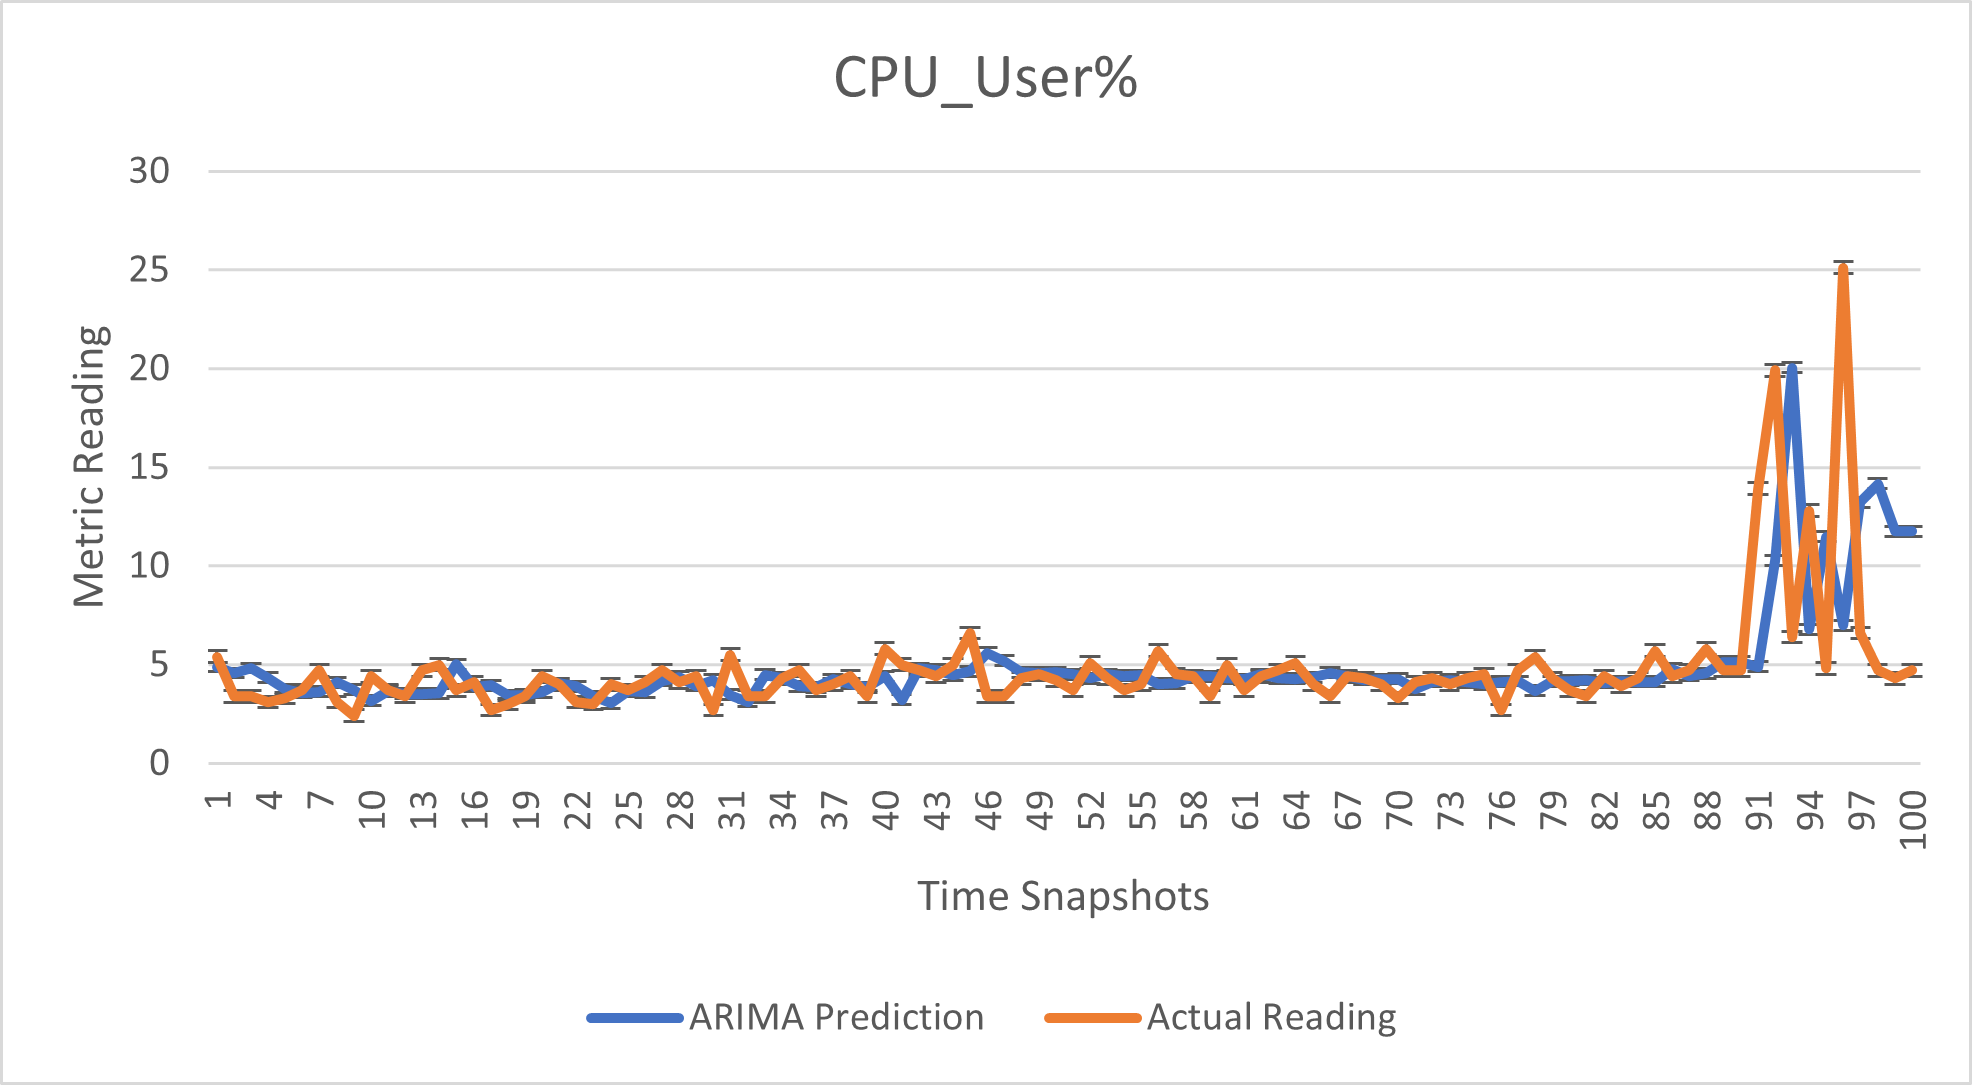
\includegraphics[width=\textwidth]{images/metrics_charts/30_pct_file_load/c1_s1/01.png}
         \caption{CPU\_User\% | ARIMA Prediction}
         \label{fig:c1_s1_01}
     \end{subfigure}
     \hfill
     \begin{subfigure}[ht]{0.32\textwidth}
         \centering
         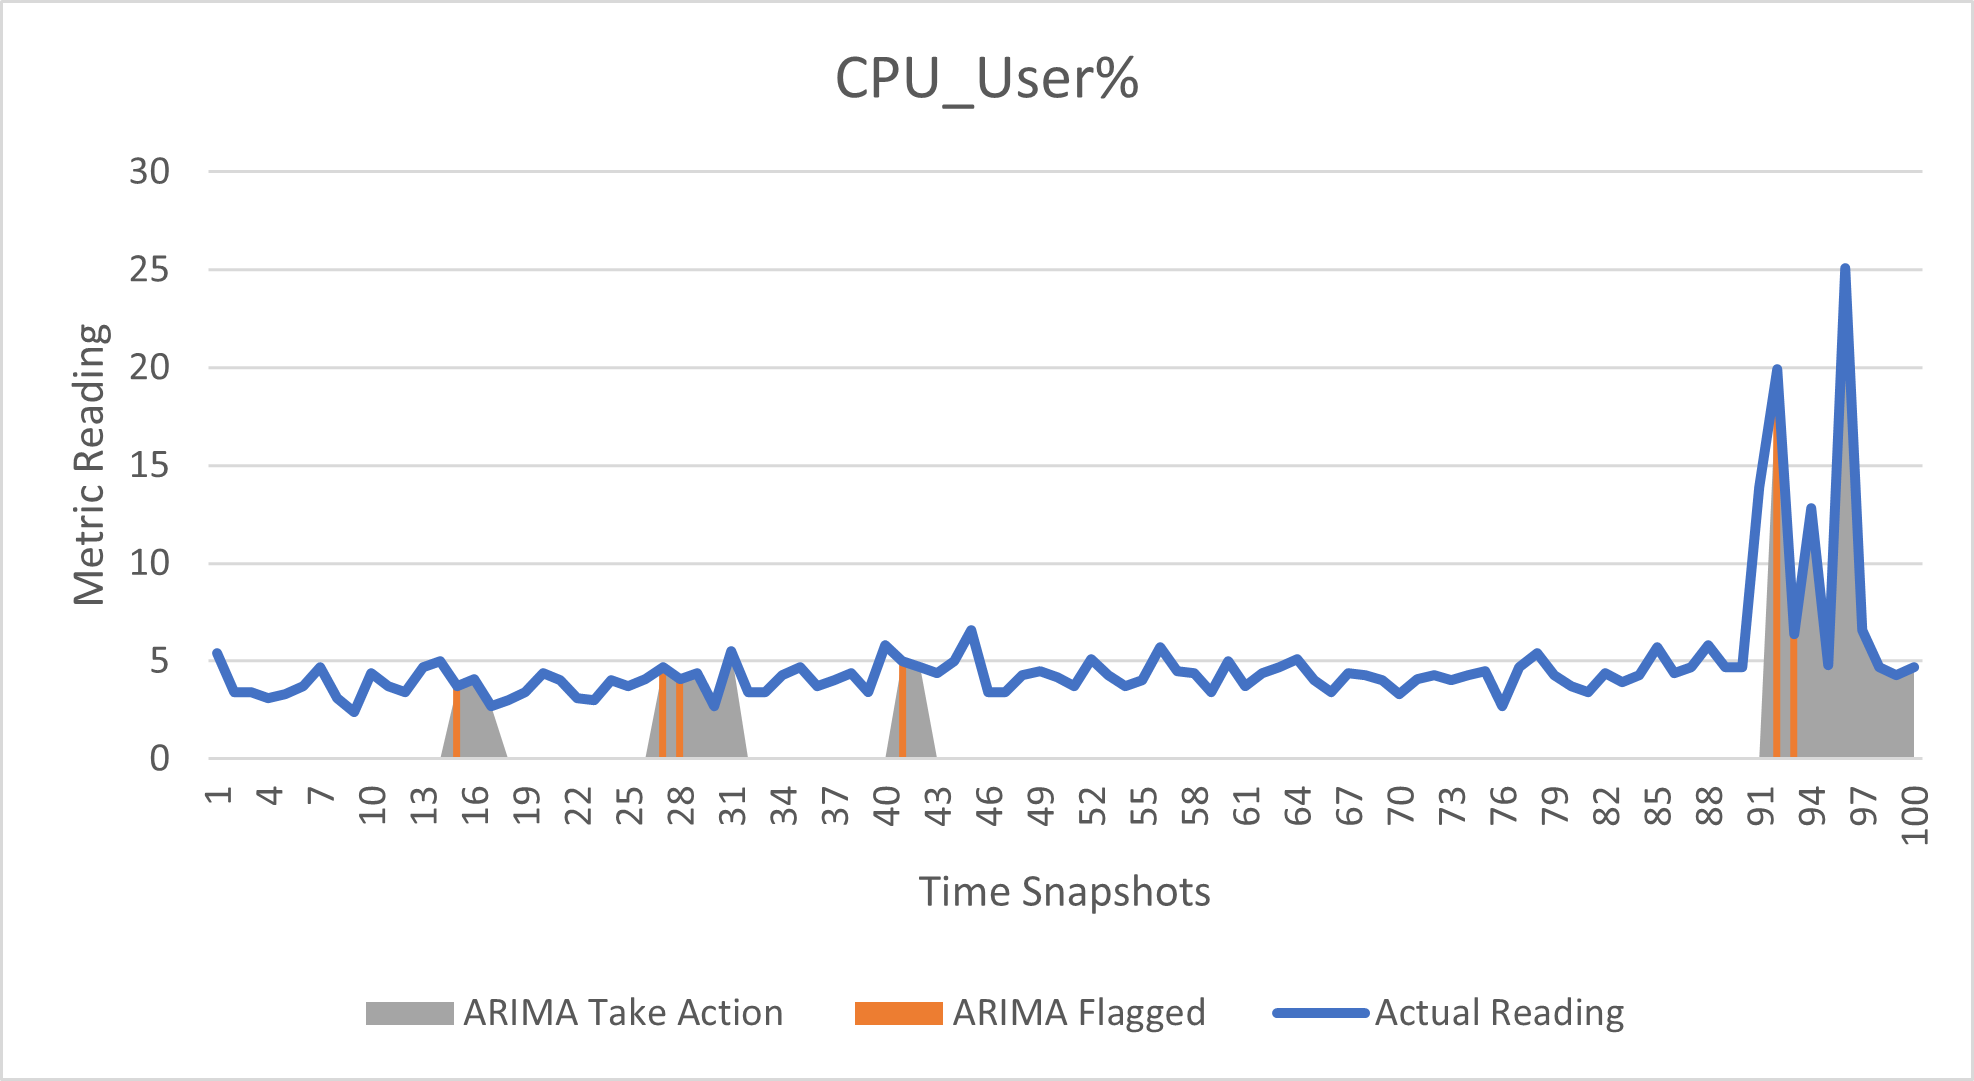
\includegraphics[width=\textwidth]{images/metrics_charts/30_pct_file_load/c1_s1/02.png}
         \caption{CPU\_User\% | Adaptive Decision}
         \label{fig:c1_s1_02}
     \end{subfigure}
     \hfill
     \begin{subfigure}[ht]{0.32\textwidth}
         \centering
         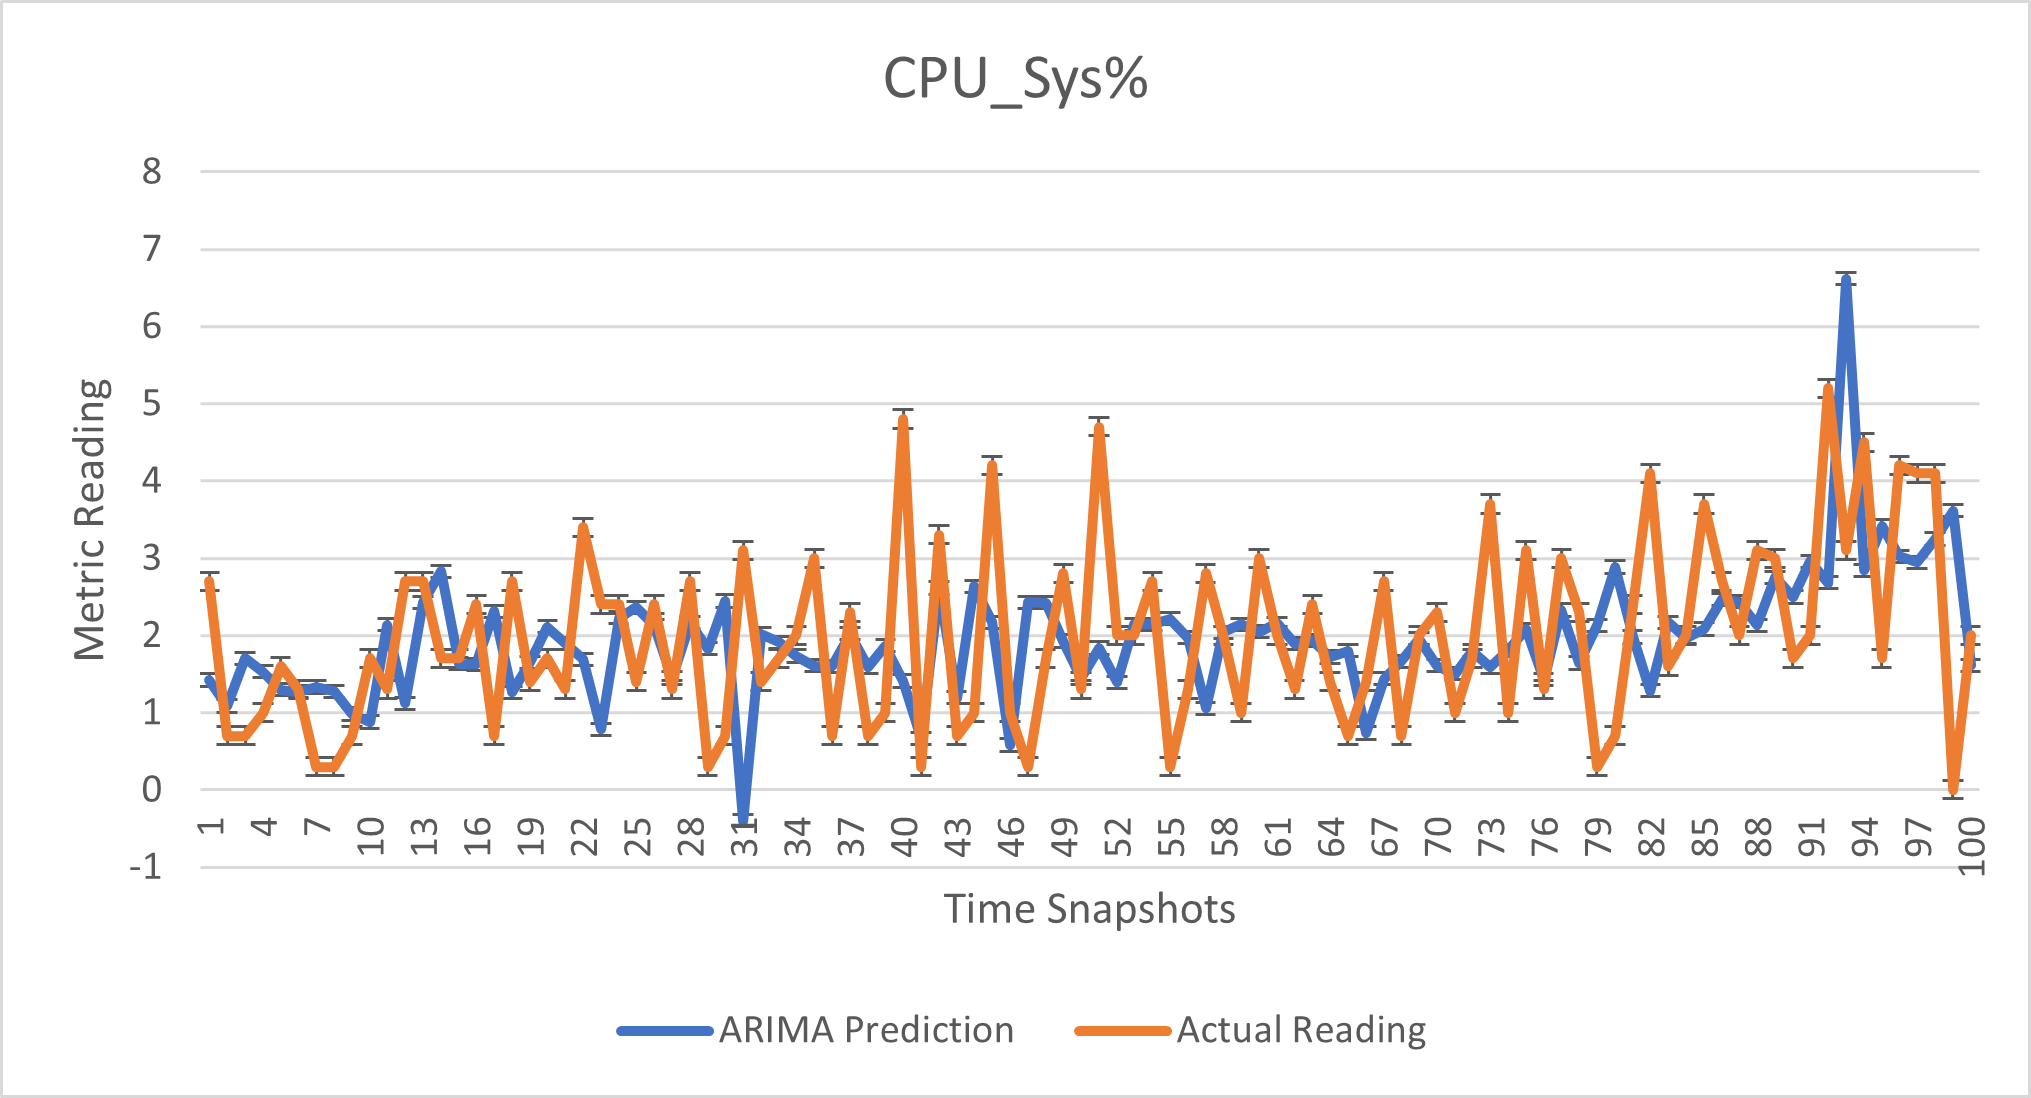
\includegraphics[width=\textwidth]{images/metrics_charts/30_pct_file_load/c1_s1/03.png}
         \caption{CPU\_Sys\% | ARIMA Prediction}
         \label{fig:c1_s1_03}
     \end{subfigure}
     \hfill
     \begin{subfigure}[ht]{0.32\textwidth}
         \centering
         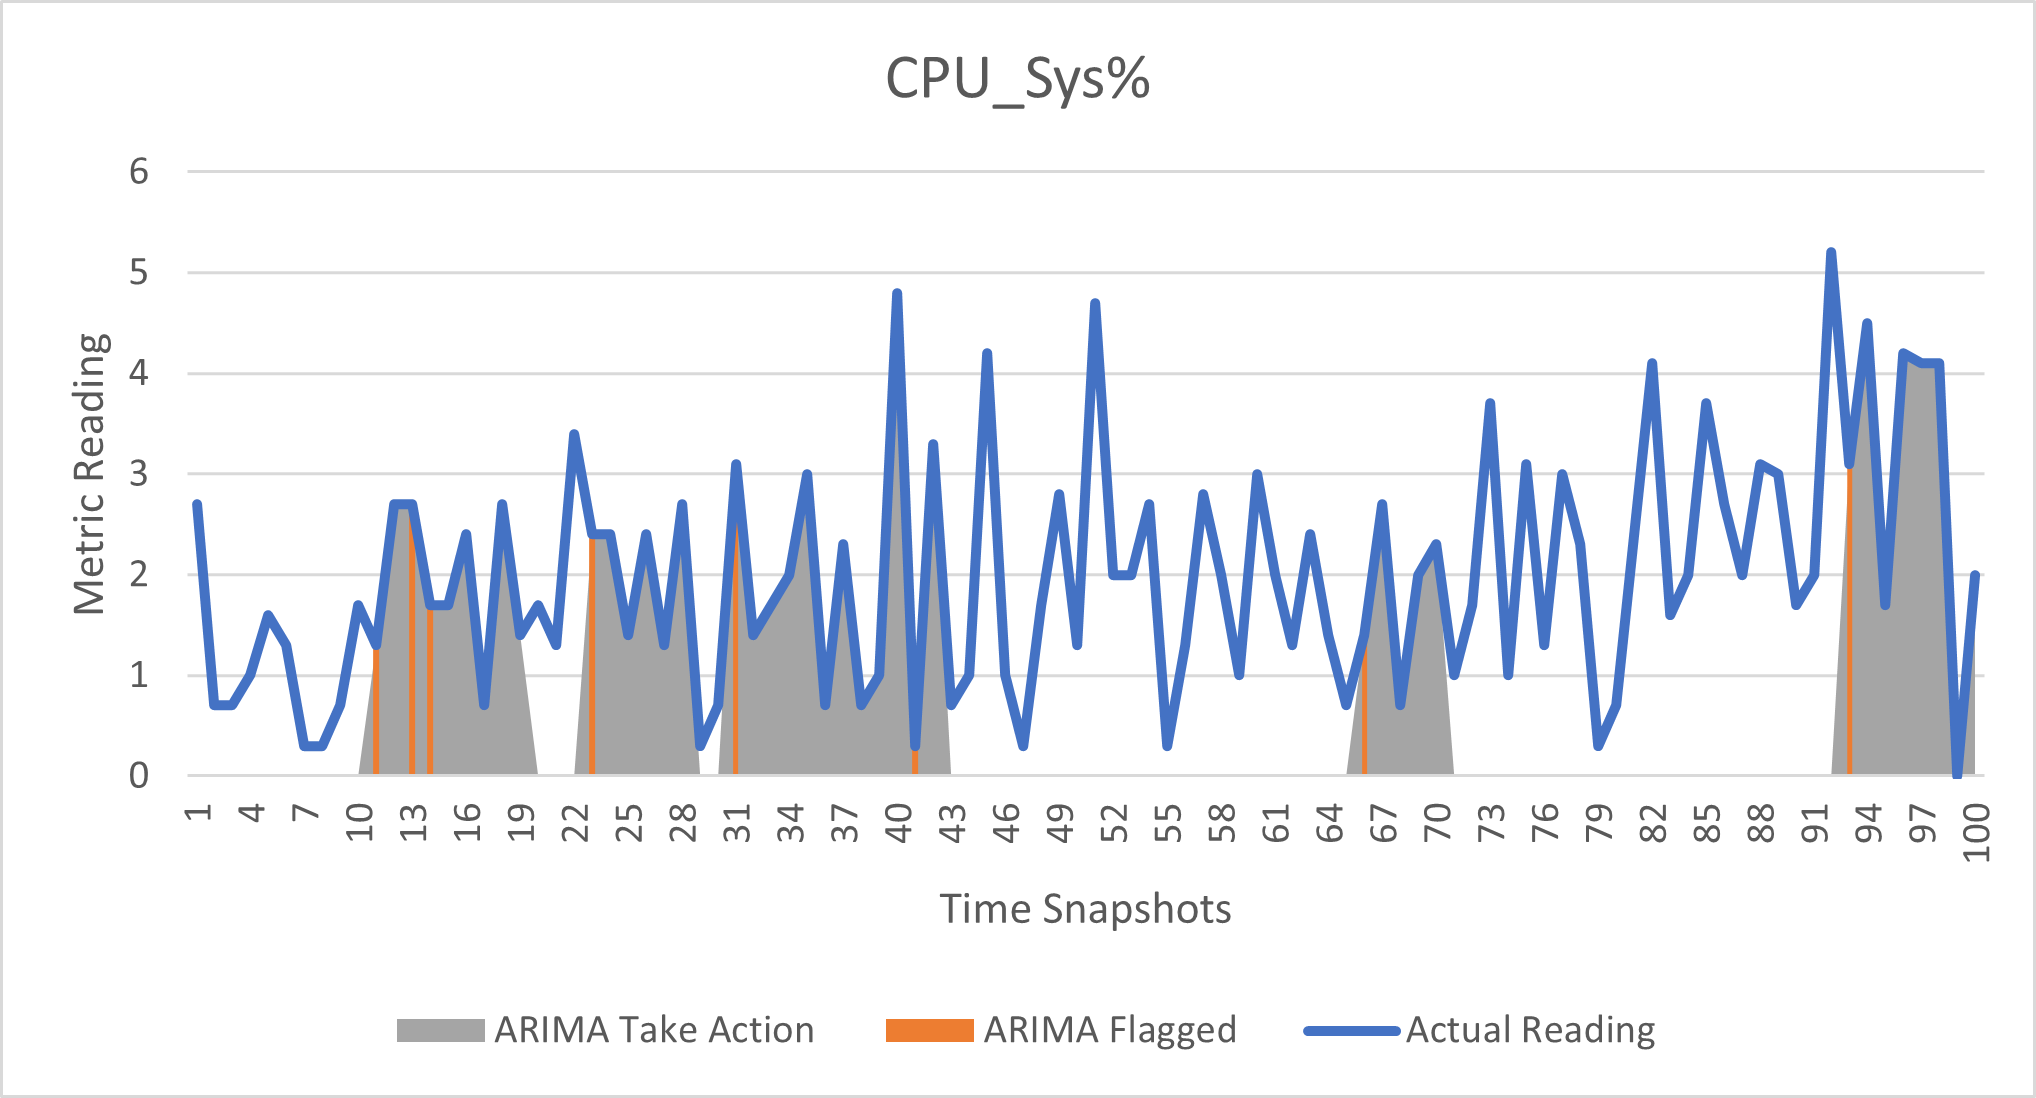
\includegraphics[width=\textwidth]{images/metrics_charts/30_pct_file_load/c1_s1/04.png}
         \caption{CPU\_Sys\% | Adaptive Decision}
         \label{fig:c1_s1_04}
     \end{subfigure}
     \hfill
     \begin{subfigure}[ht]{0.32\textwidth}
         \centering
         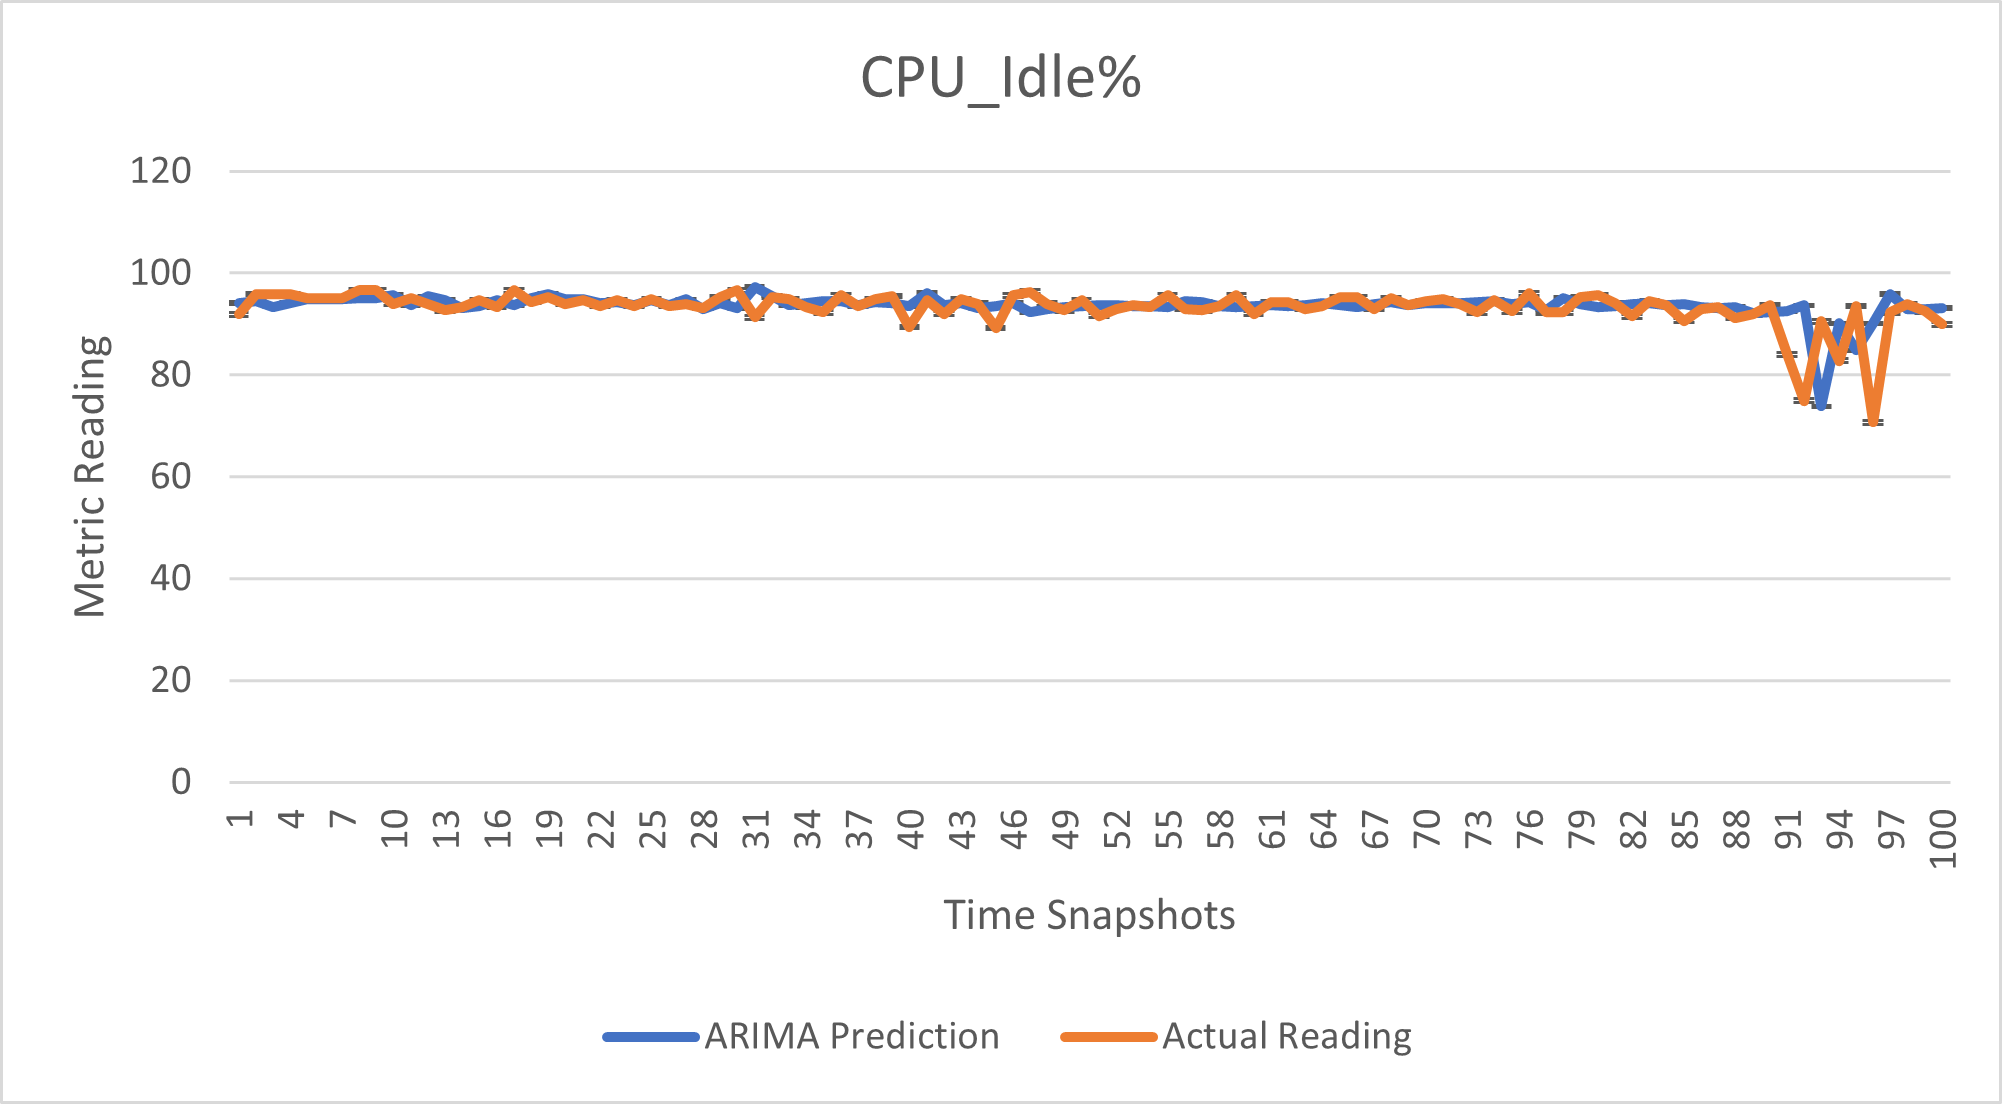
\includegraphics[width=\textwidth]{images/metrics_charts/30_pct_file_load/c1_s1/05.png}
         \caption{CPU\_Idle\% | ARIMA Prediction}
         \label{fig:c1_s1_05}
     \end{subfigure}
     \hfill
     \begin{subfigure}[ht]{0.32\textwidth}
         \centering
         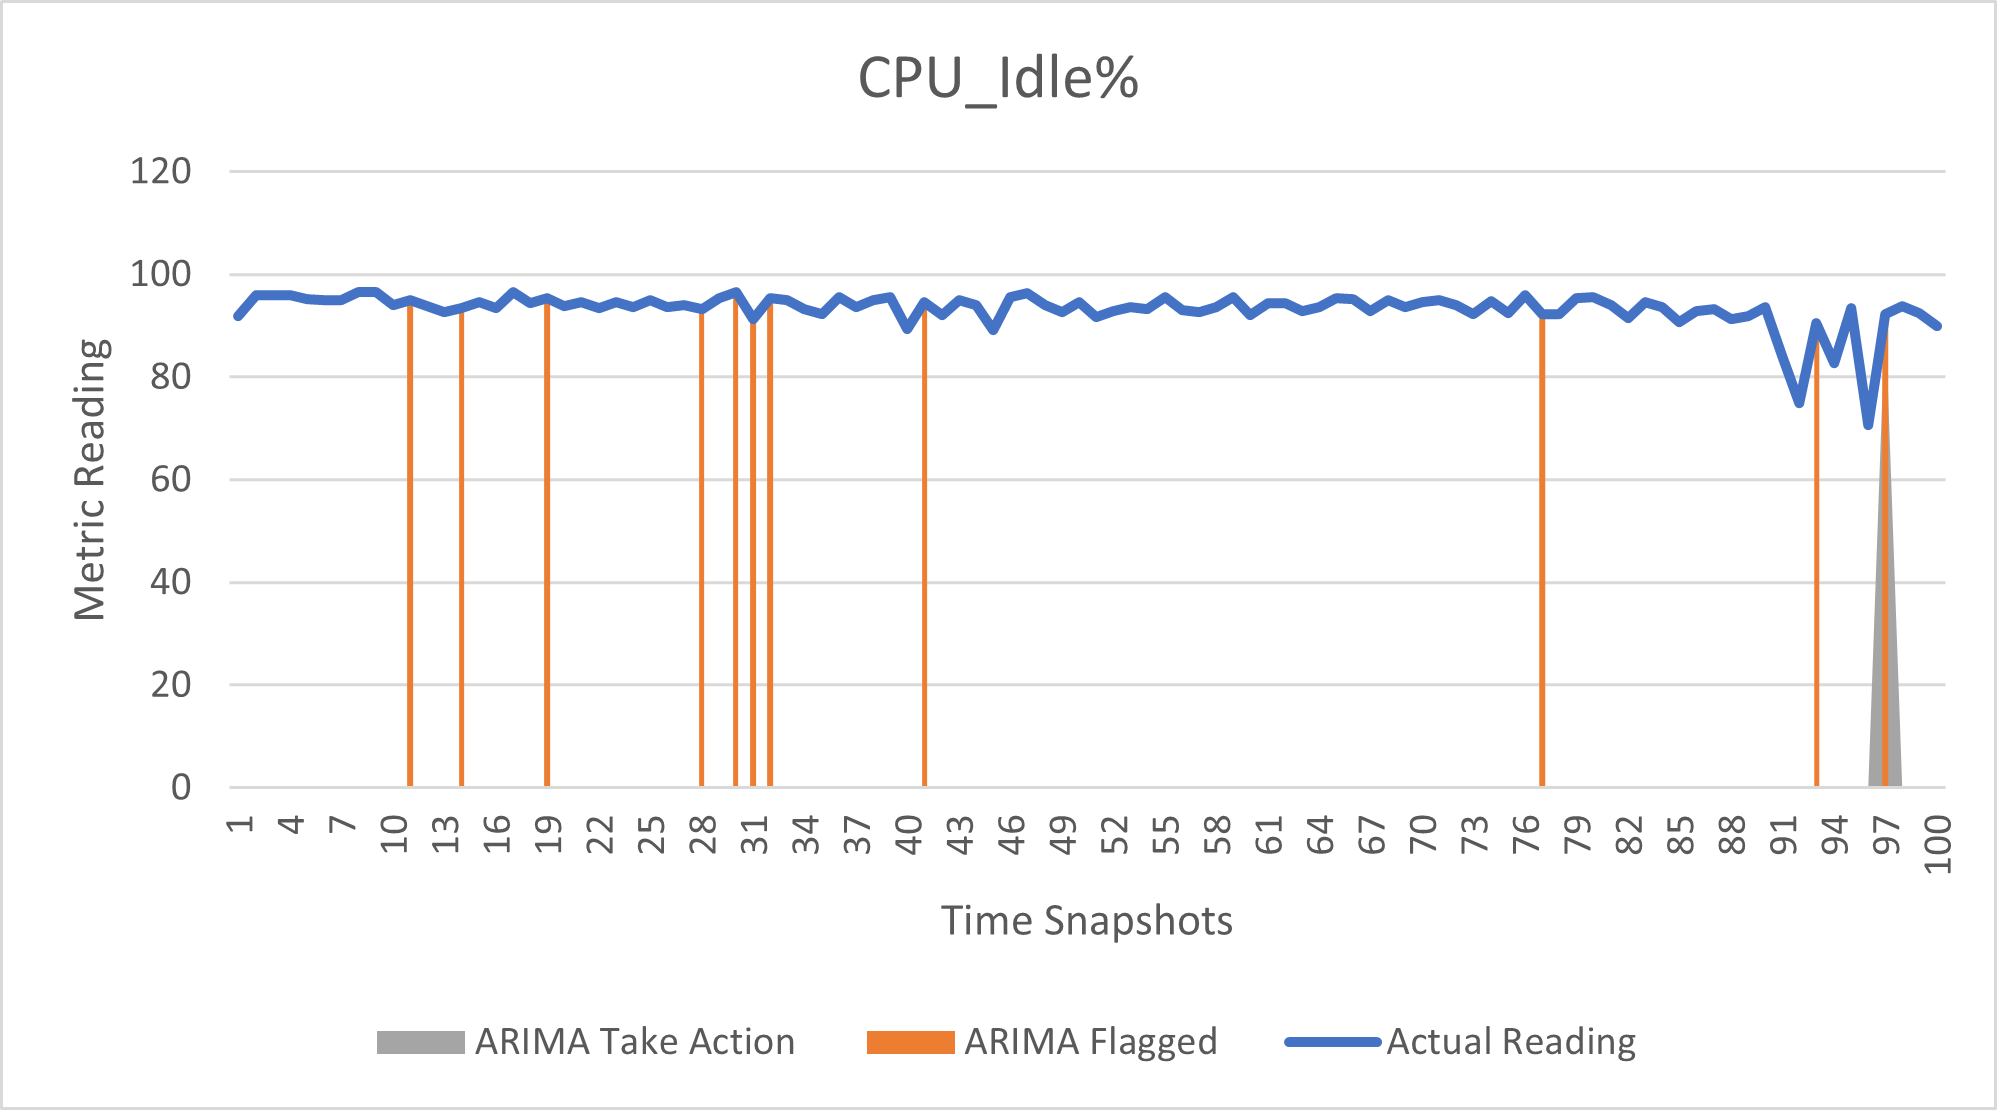
\includegraphics[width=\textwidth]{images/metrics_charts/30_pct_file_load/c1_s1/06.png}
         \caption{CPU\_Idle\% | Adaptive Decision}
         \label{fig:c1_s1_06}
     \end{subfigure}
     \hfill
     \begin{subfigure}[ht]{0.32\textwidth}
         \centering
         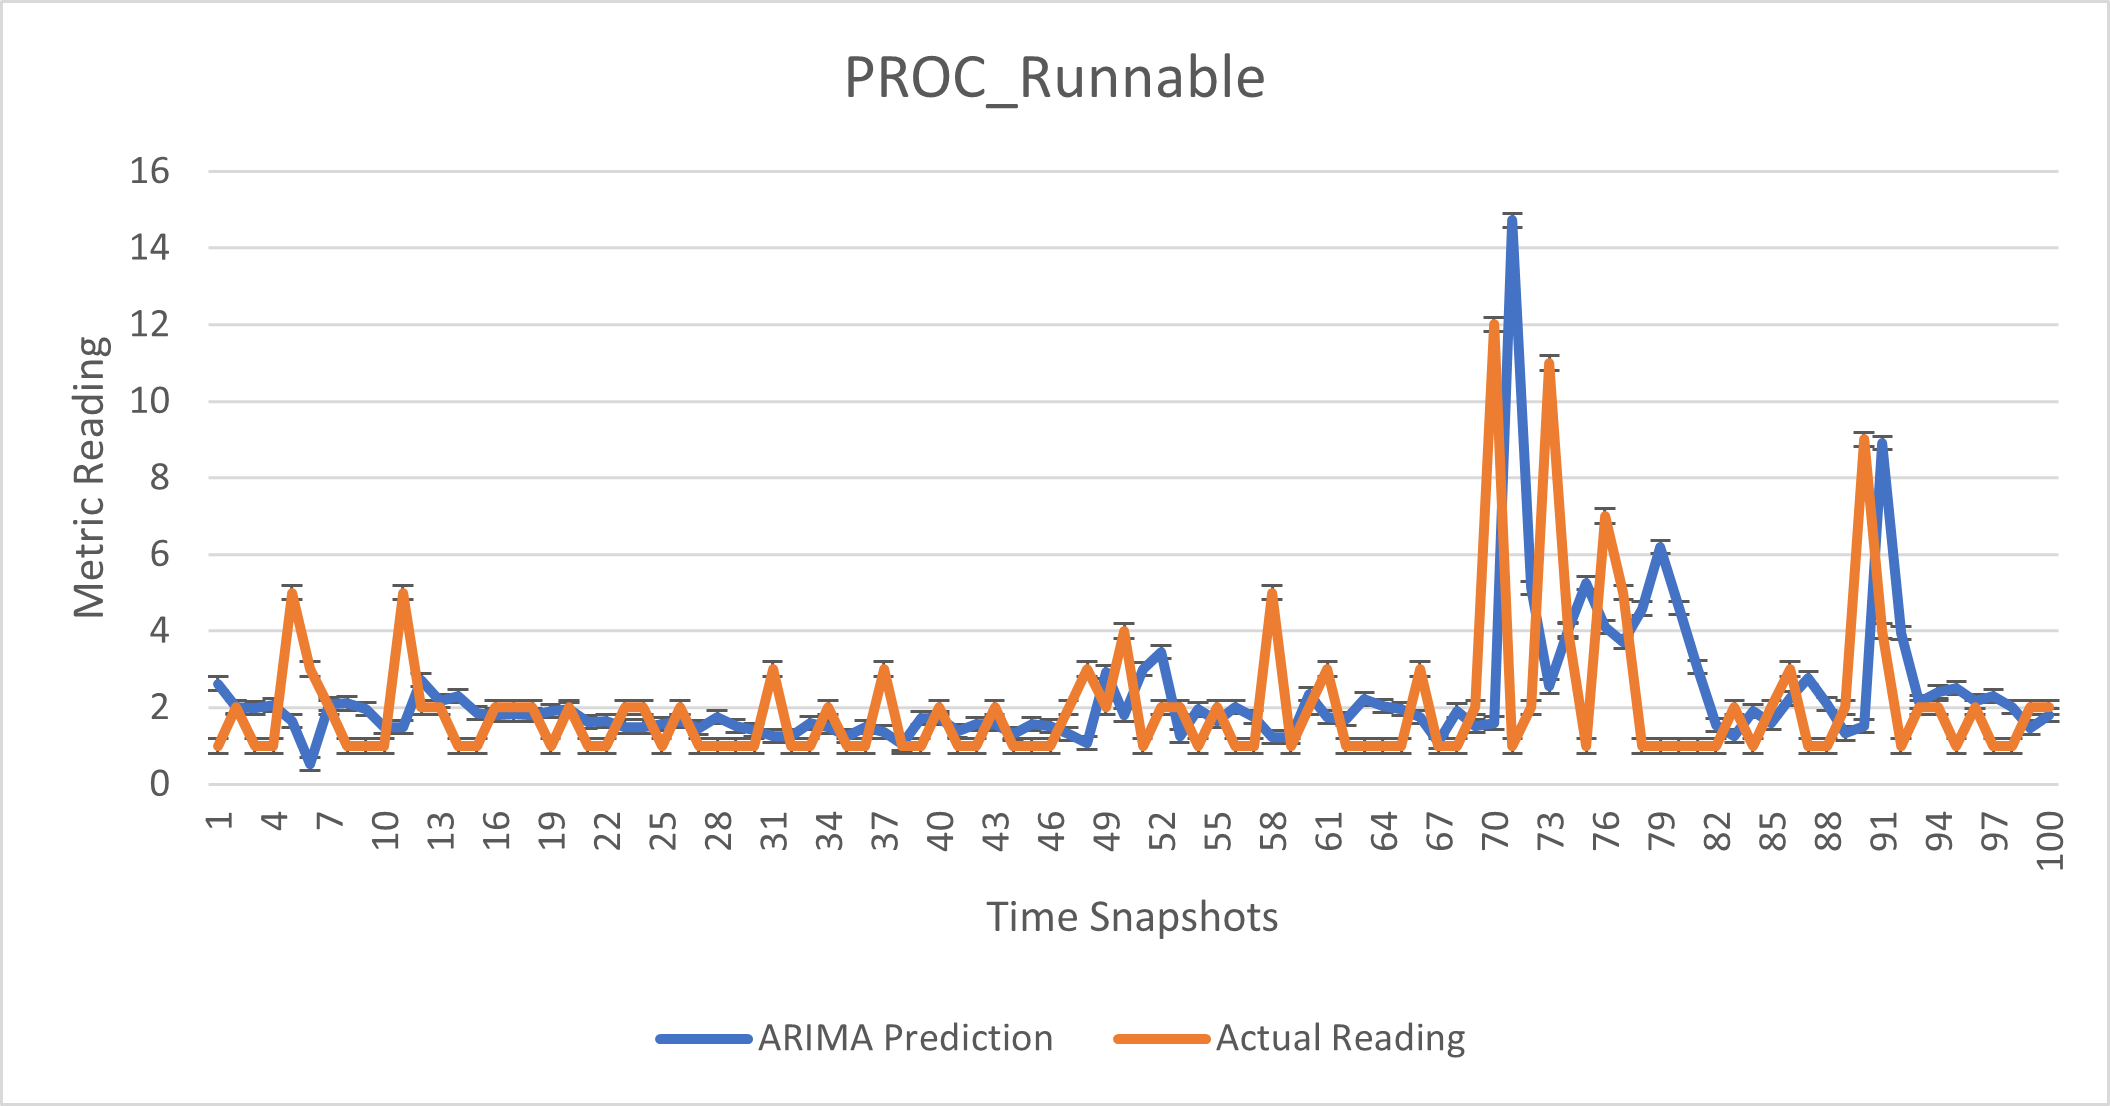
\includegraphics[width=\textwidth]{images/metrics_charts/30_pct_file_load/c1_s1/07.png}
         \caption{PROC\_Runnable | ARIMA Prediction}
         \label{fig:c1_s1_07}
     \end{subfigure}
     \hfill
     \begin{subfigure}[ht]{0.32\textwidth}
         \centering
         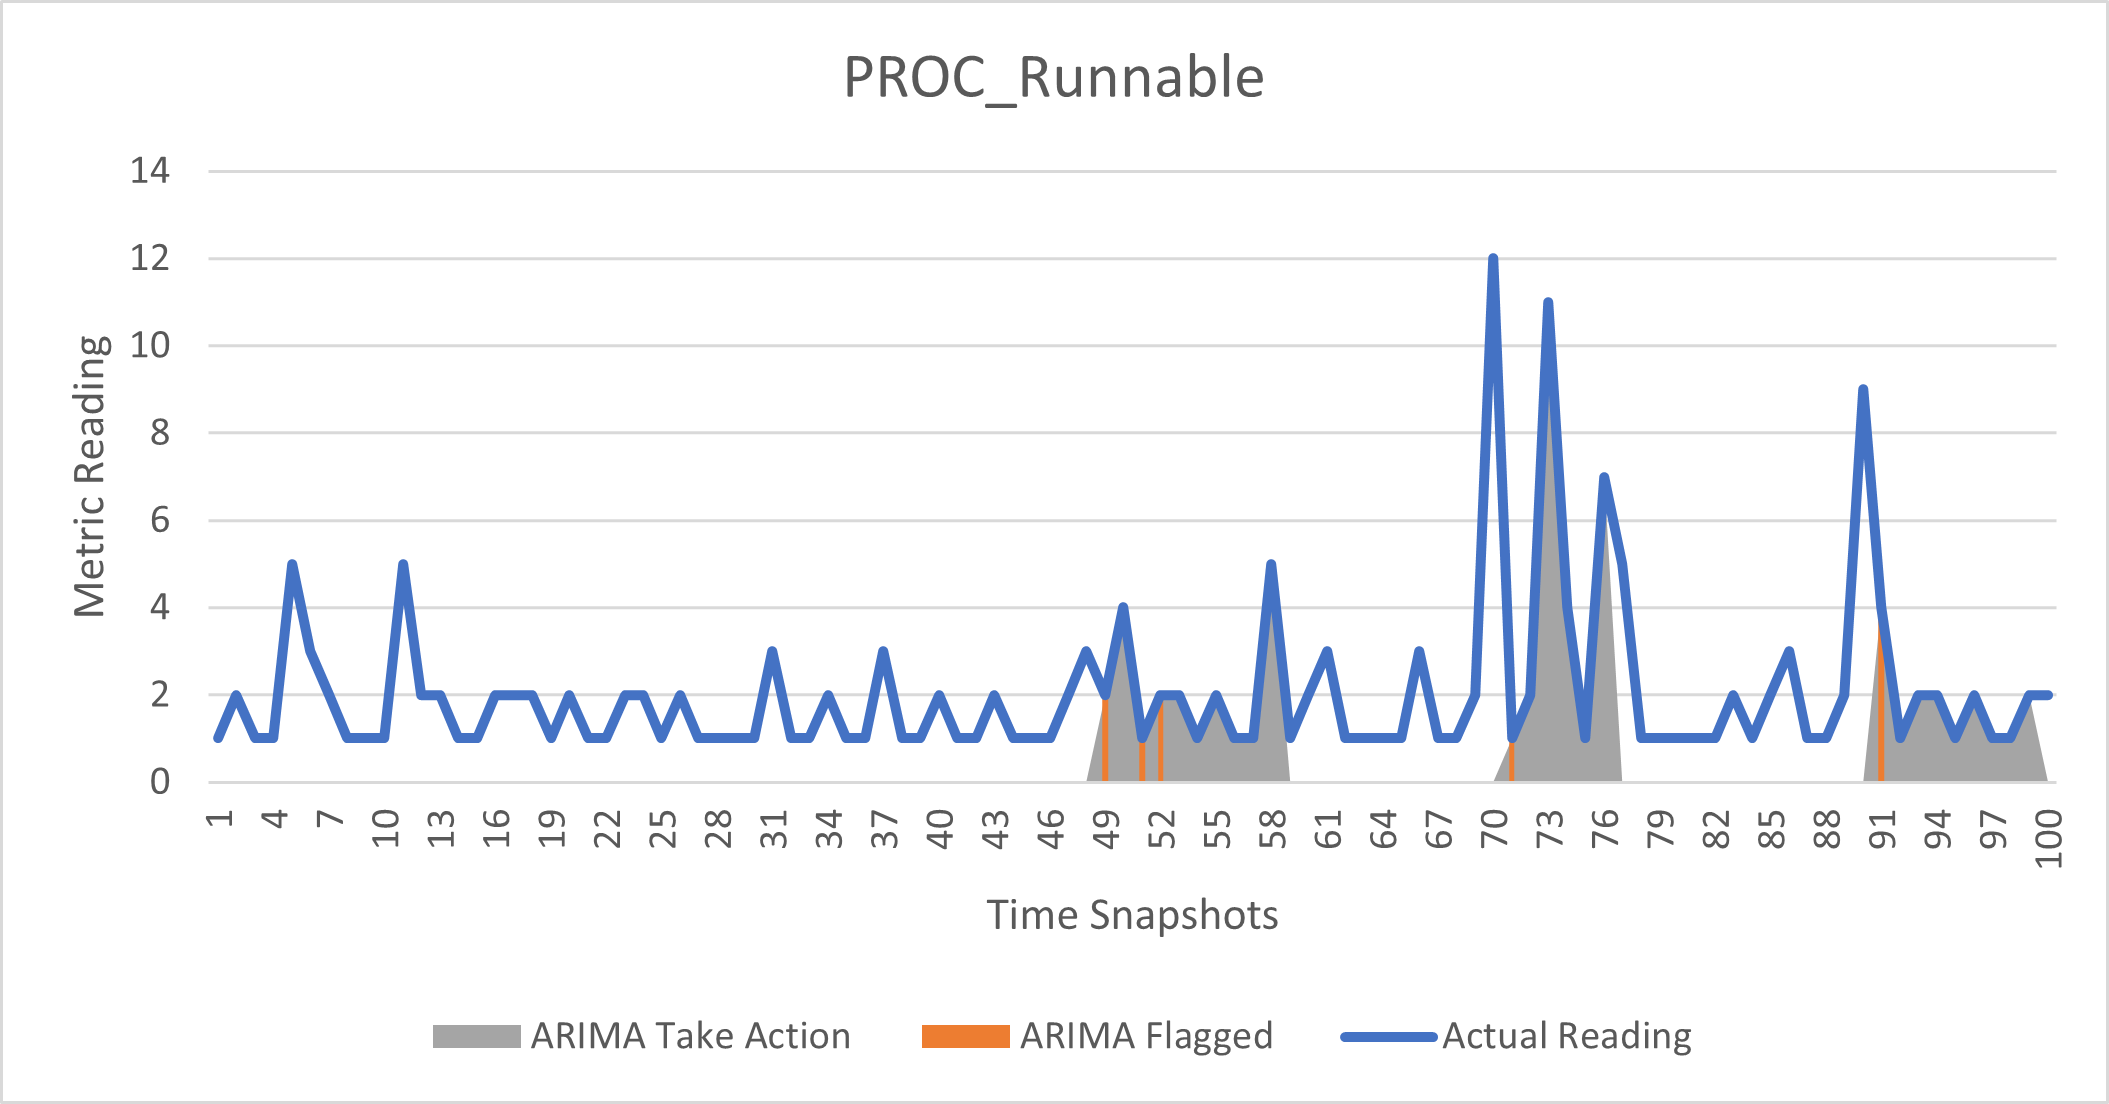
\includegraphics[width=\textwidth]{images/metrics_charts/30_pct_file_load/c1_s1/08.png}
         \caption{PROC\_Runnable | Adaptive Decision}
         \label{fig:c1_s1_08}
     \end{subfigure}
     \hfill
     \begin{subfigure}[ht]{0.32\textwidth}
         \centering
         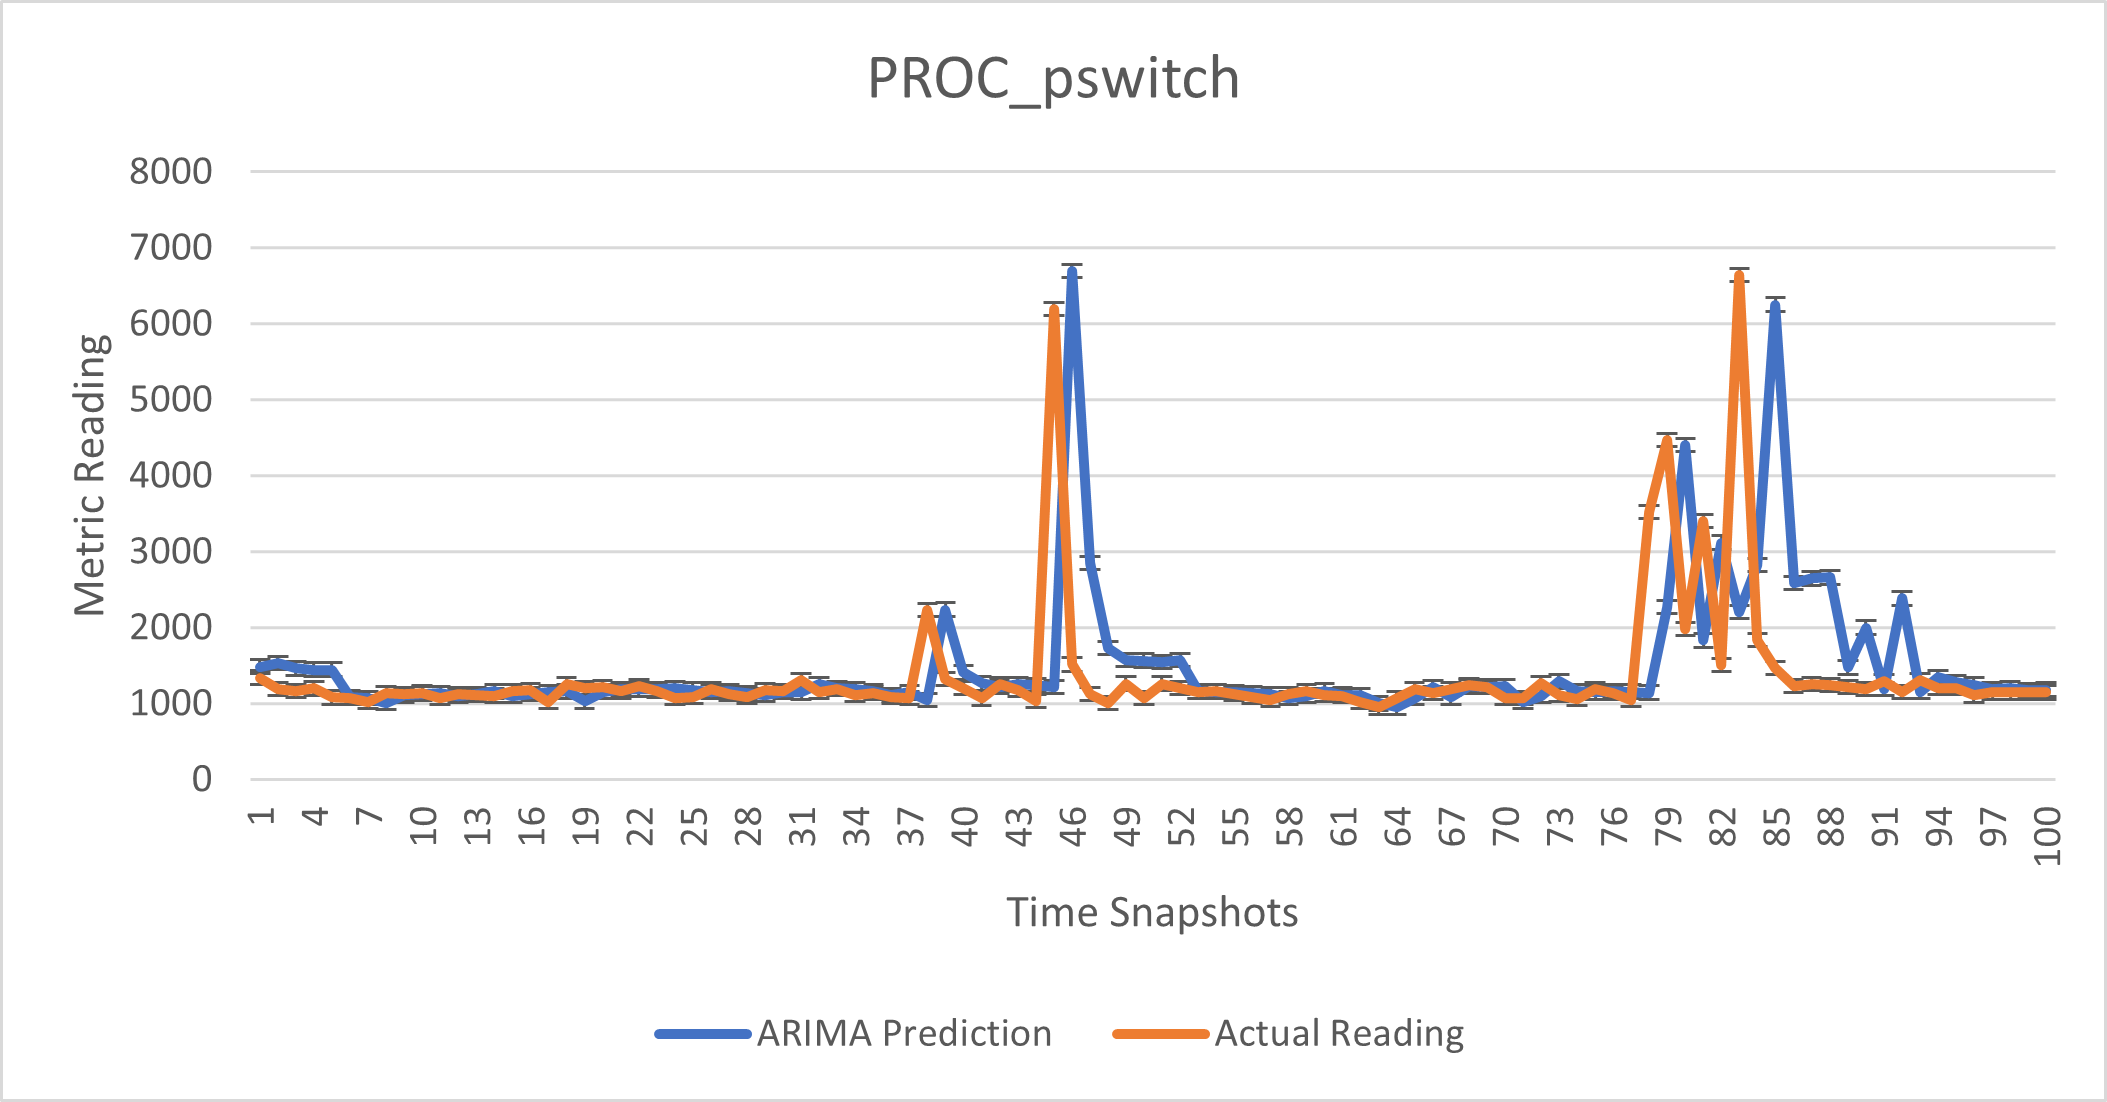
\includegraphics[width=\textwidth]{images/metrics_charts/30_pct_file_load/c1_s1/09.png}
         \caption{PROC\_pswitch | ARIMA Prediction}
         \label{fig:c1_s1_09}
     \end{subfigure}
     \hfill
     \begin{subfigure}[ht]{0.32\textwidth}
         \centering
         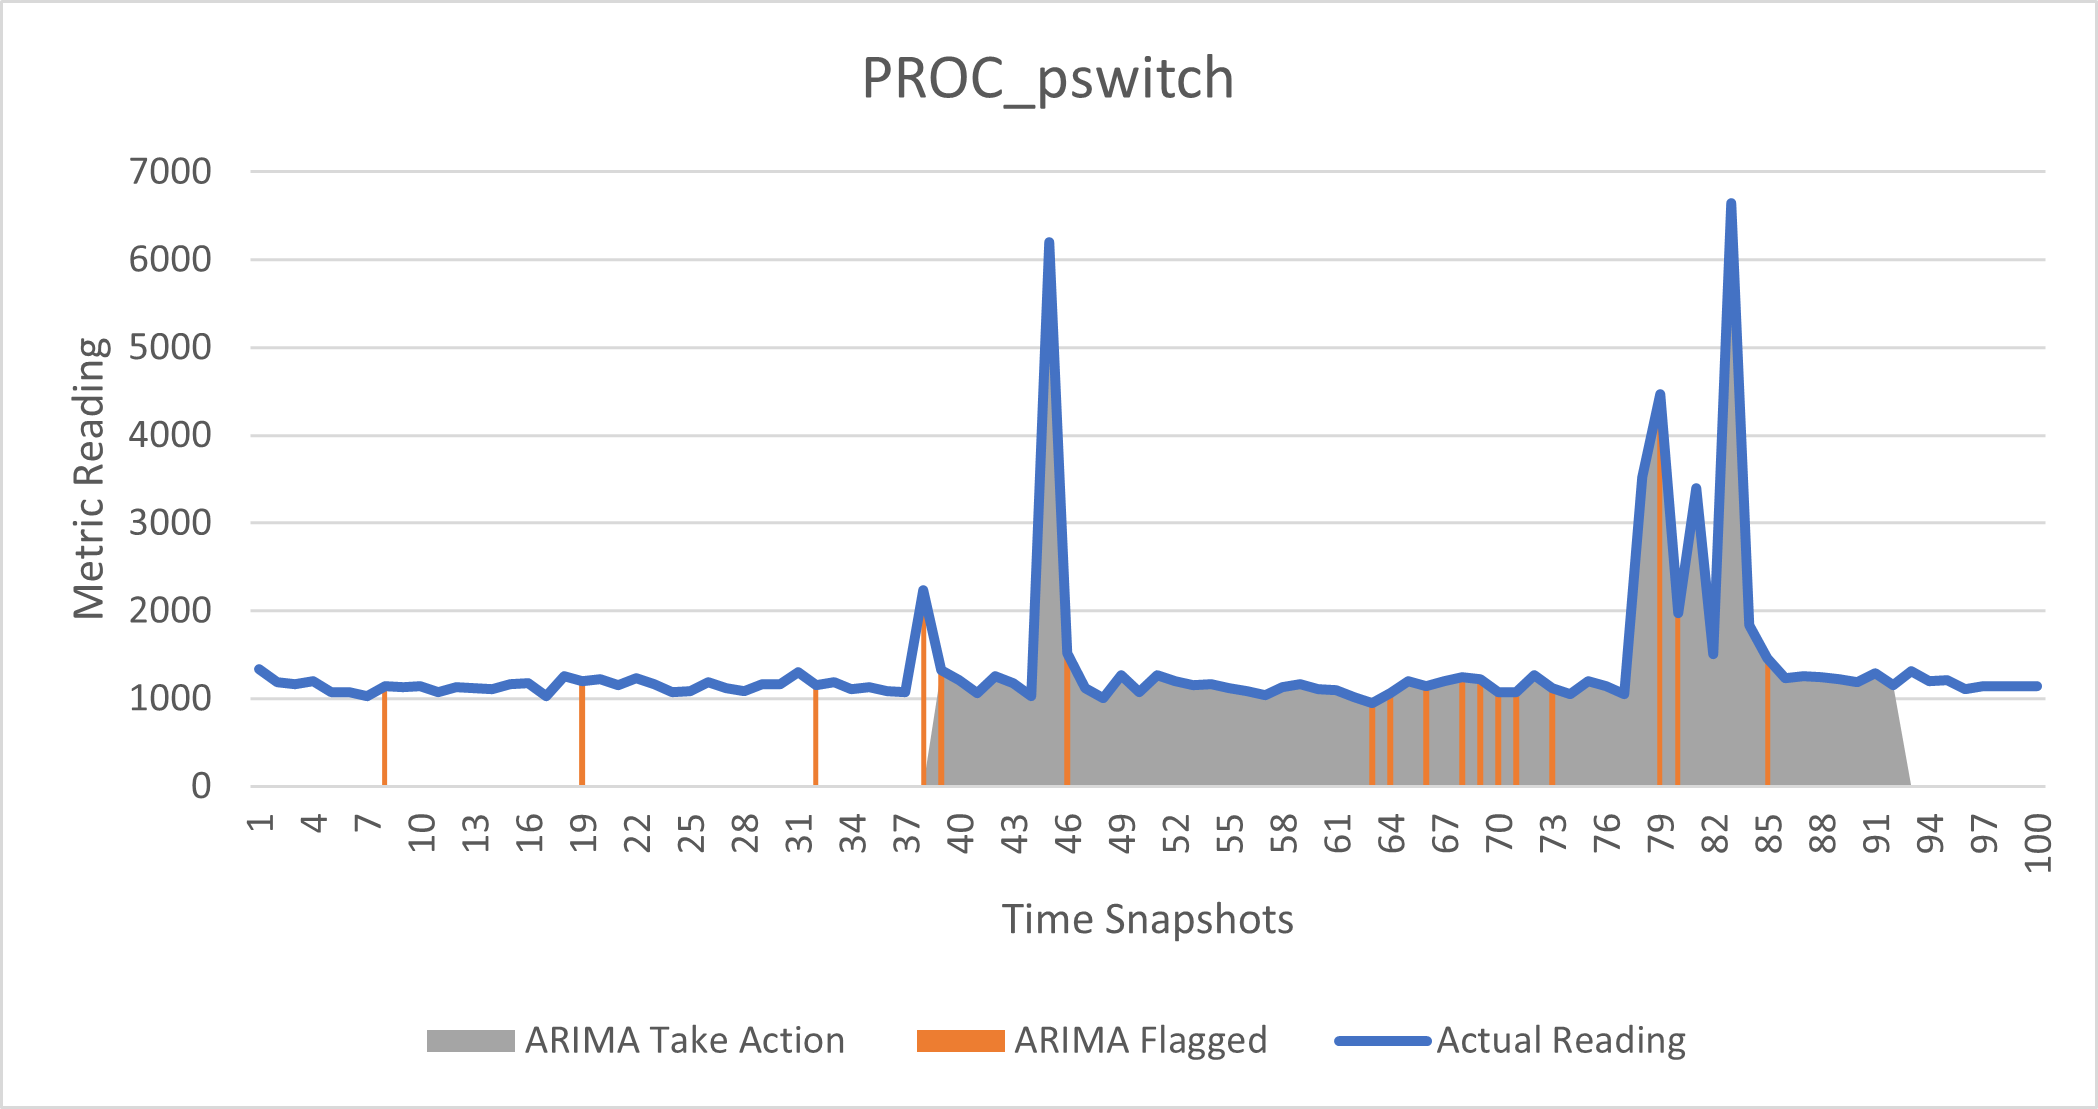
\includegraphics[width=\textwidth]{images/metrics_charts/30_pct_file_load/c1_s1/10.png}
         \caption{PROC\_pswitch  | Adaptive Decision}
         \label{fig:c1_s1_10}
     \end{subfigure}
     \hfill
     \caption{CPU Metrics | Case Study: 1}
     \label{fig:c1_s1_cpu}
\end{figure*}

Figure \ref{fig:c1_s1_memory} shows the memory-related metrics that were flagged during this experiment. VM\_nr\_dirty metric has seen many trend changes in Figure \ref{fig:c1_s1_12}. If we observe the ARIMA flags and the take-action areas suggested by our proposed approach, it is obvious that this metric was the most problematic out of all the 21 metrics. VM\_pageout has seen some large spikes, as seen in Figure \ref{fig:c1_s1_14}. However, as the frequency of the spikes was relatively low (just 3\%); therefore we could see this metric was not flagged as much. VM\_pgfree and VM\_pgfault have seen a similar number of flags and action-taking suggestions. Overall, from the memory-related metrics, we can observe that VM\_nr\_dirty was affected the most. This is in line with the tasks that were performed in the experiment, as the number of prime numbers generated was increasing every time; therefore apache cache for that webpage (the PHP script) had to be modified all the time, which affected the system performance in serving back the page.

\begin{figure*}[tbp]
     \centering
     \begin{subfigure}[ht]{0.32\textwidth}
         \centering
         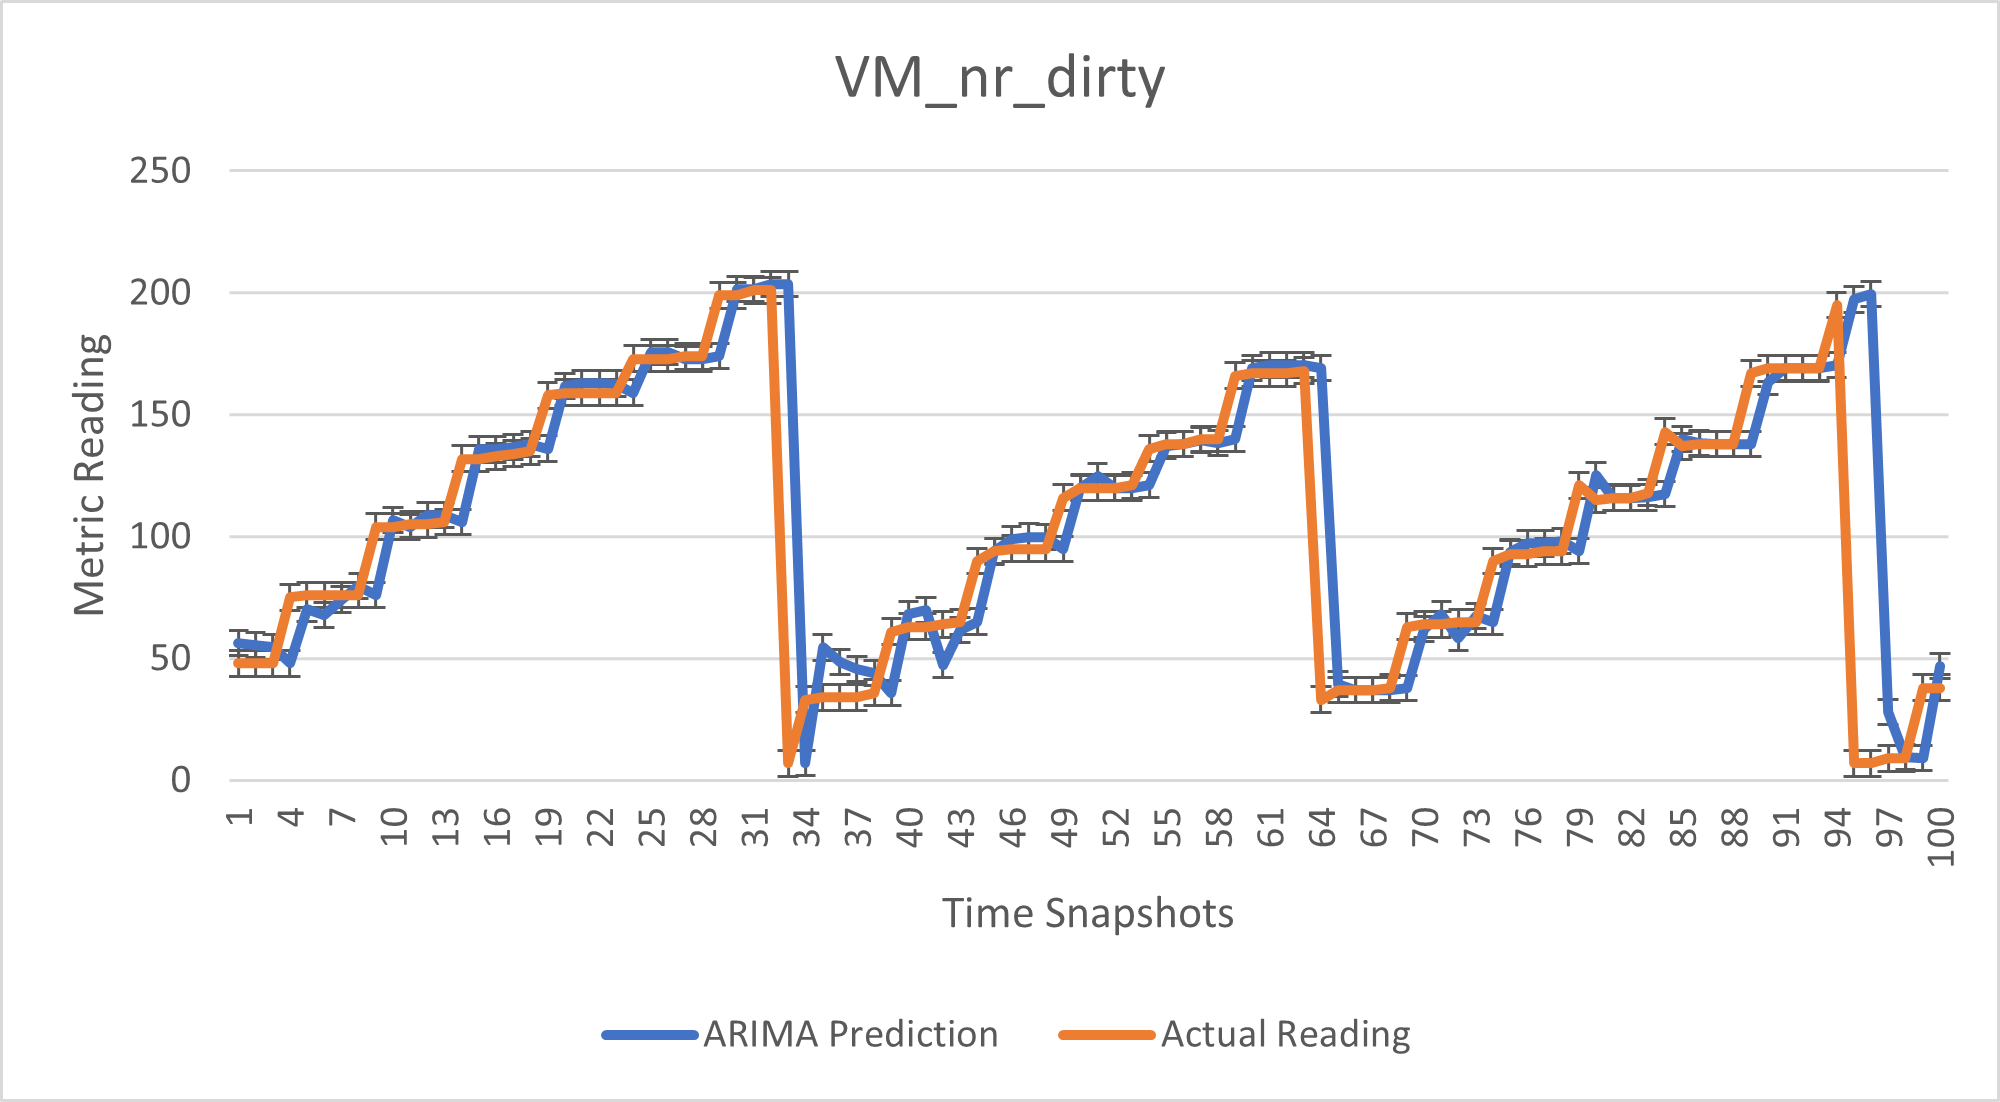
\includegraphics[width=\textwidth]{images/metrics_charts/30_pct_file_load/c1_s1/11.png}
         \caption{VM\_nr\_dirty | ARIMA Prediction}
         \label{fig:c1_s1_11}
     \end{subfigure}
     \hfill
     \begin{subfigure}[ht]{0.32\textwidth}
         \centering
         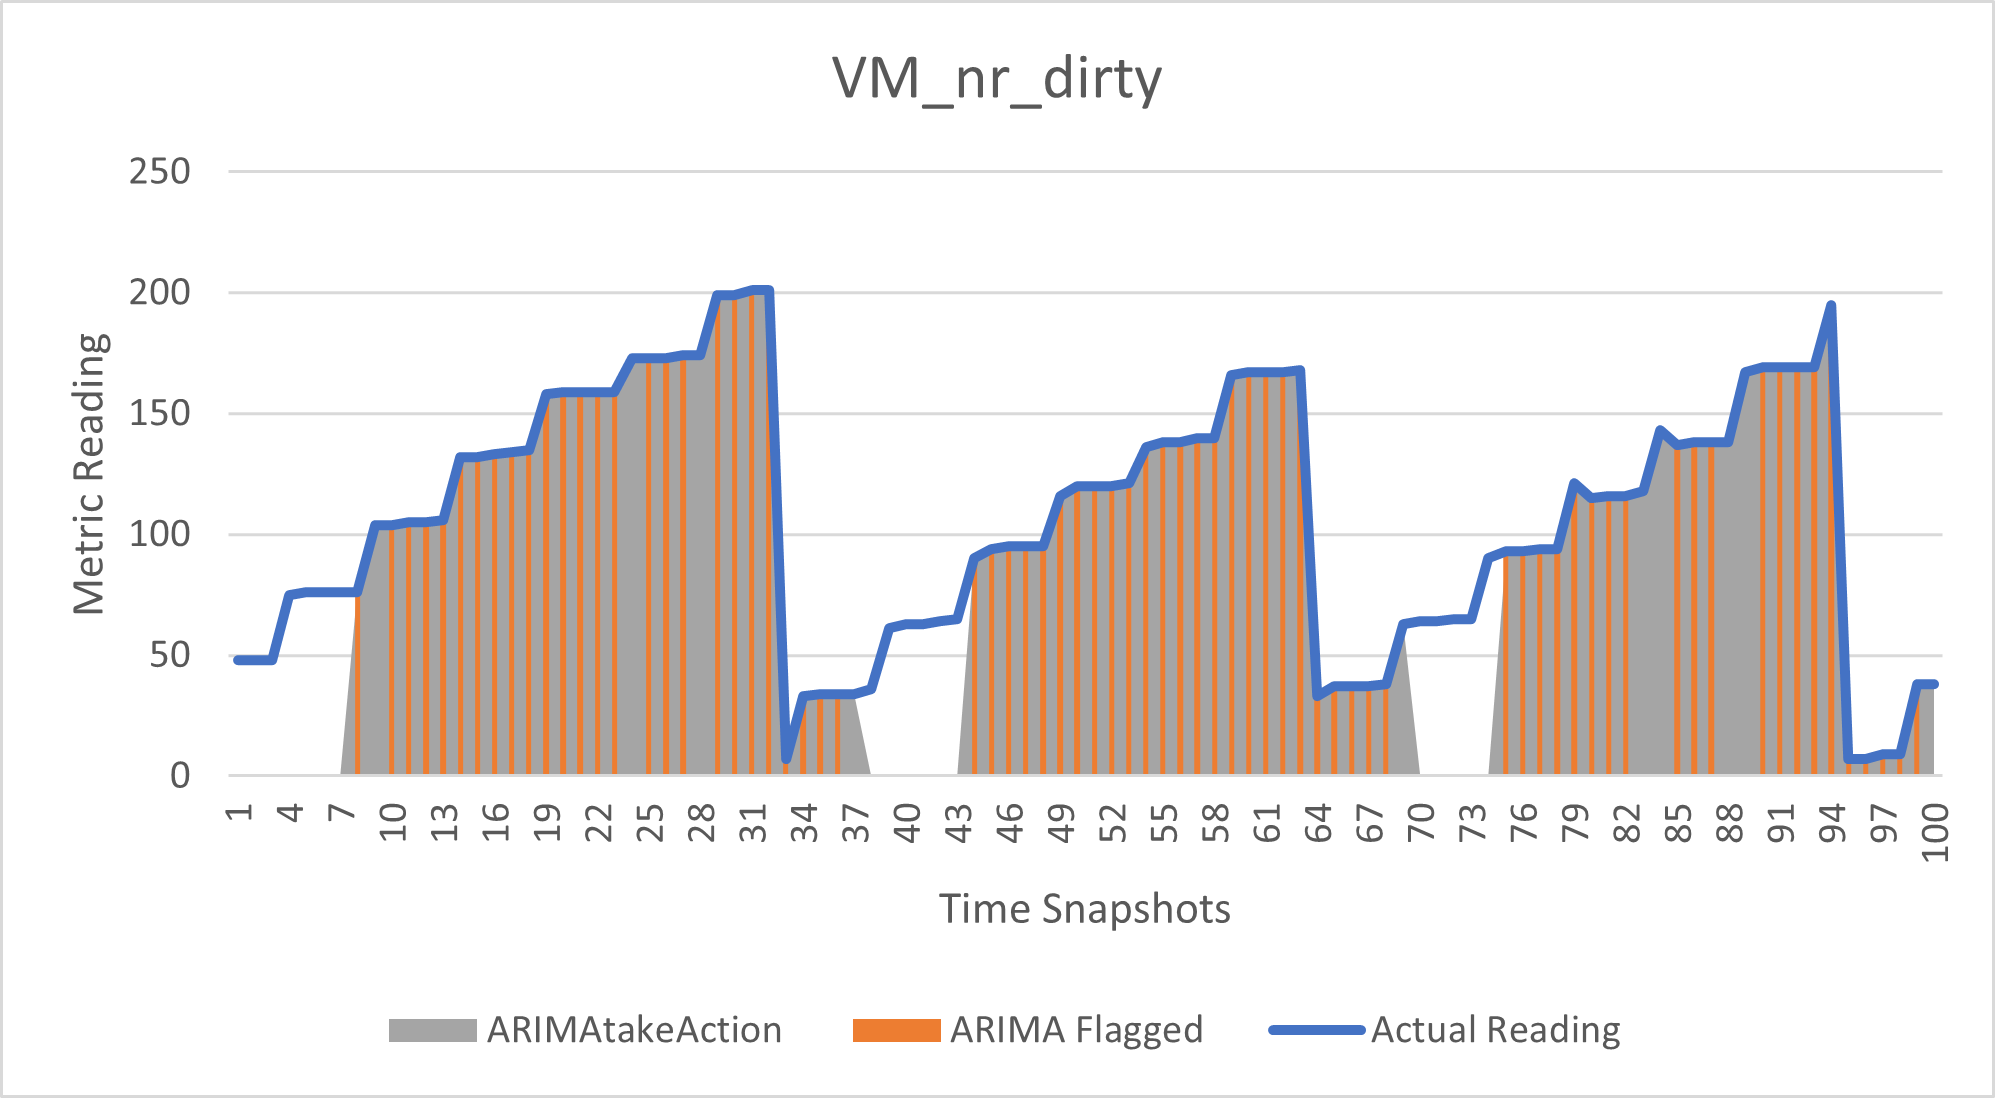
\includegraphics[width=\textwidth]{images/metrics_charts/30_pct_file_load/c1_s1/12.png}
         \caption{VM\_nr\_dirty | Adaptive Decision}
         \label{fig:c1_s1_12}
     \end{subfigure}
     \hfill
     \begin{subfigure}[ht]{0.32\textwidth}
         \centering
         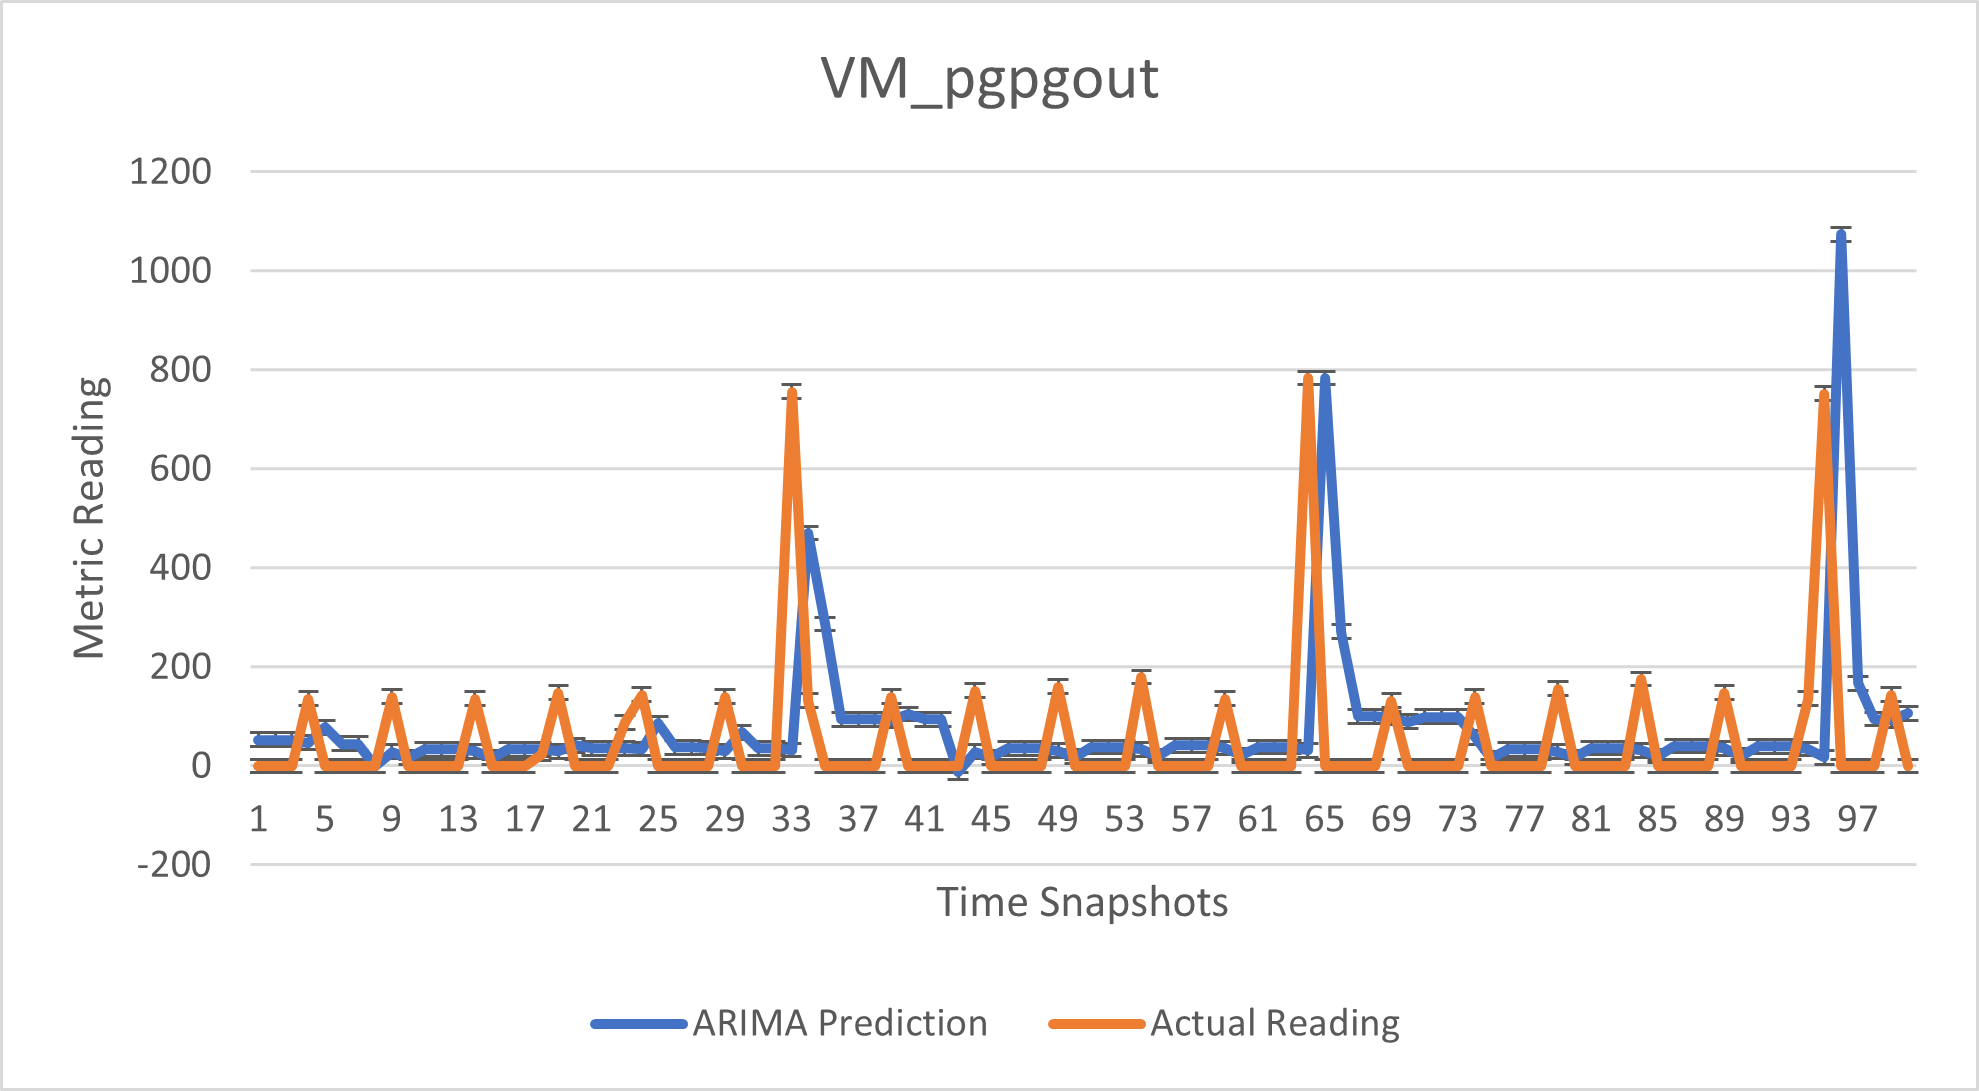
\includegraphics[width=\textwidth]{images/metrics_charts/30_pct_file_load/c1_s1/13.png}
         \caption{VM\_pageout | ARIMA Prediction}
         \label{fig:c1_s1_13}
     \end{subfigure}
     \hfill   
     \begin{subfigure}[ht]{0.32\textwidth}
         \centering
         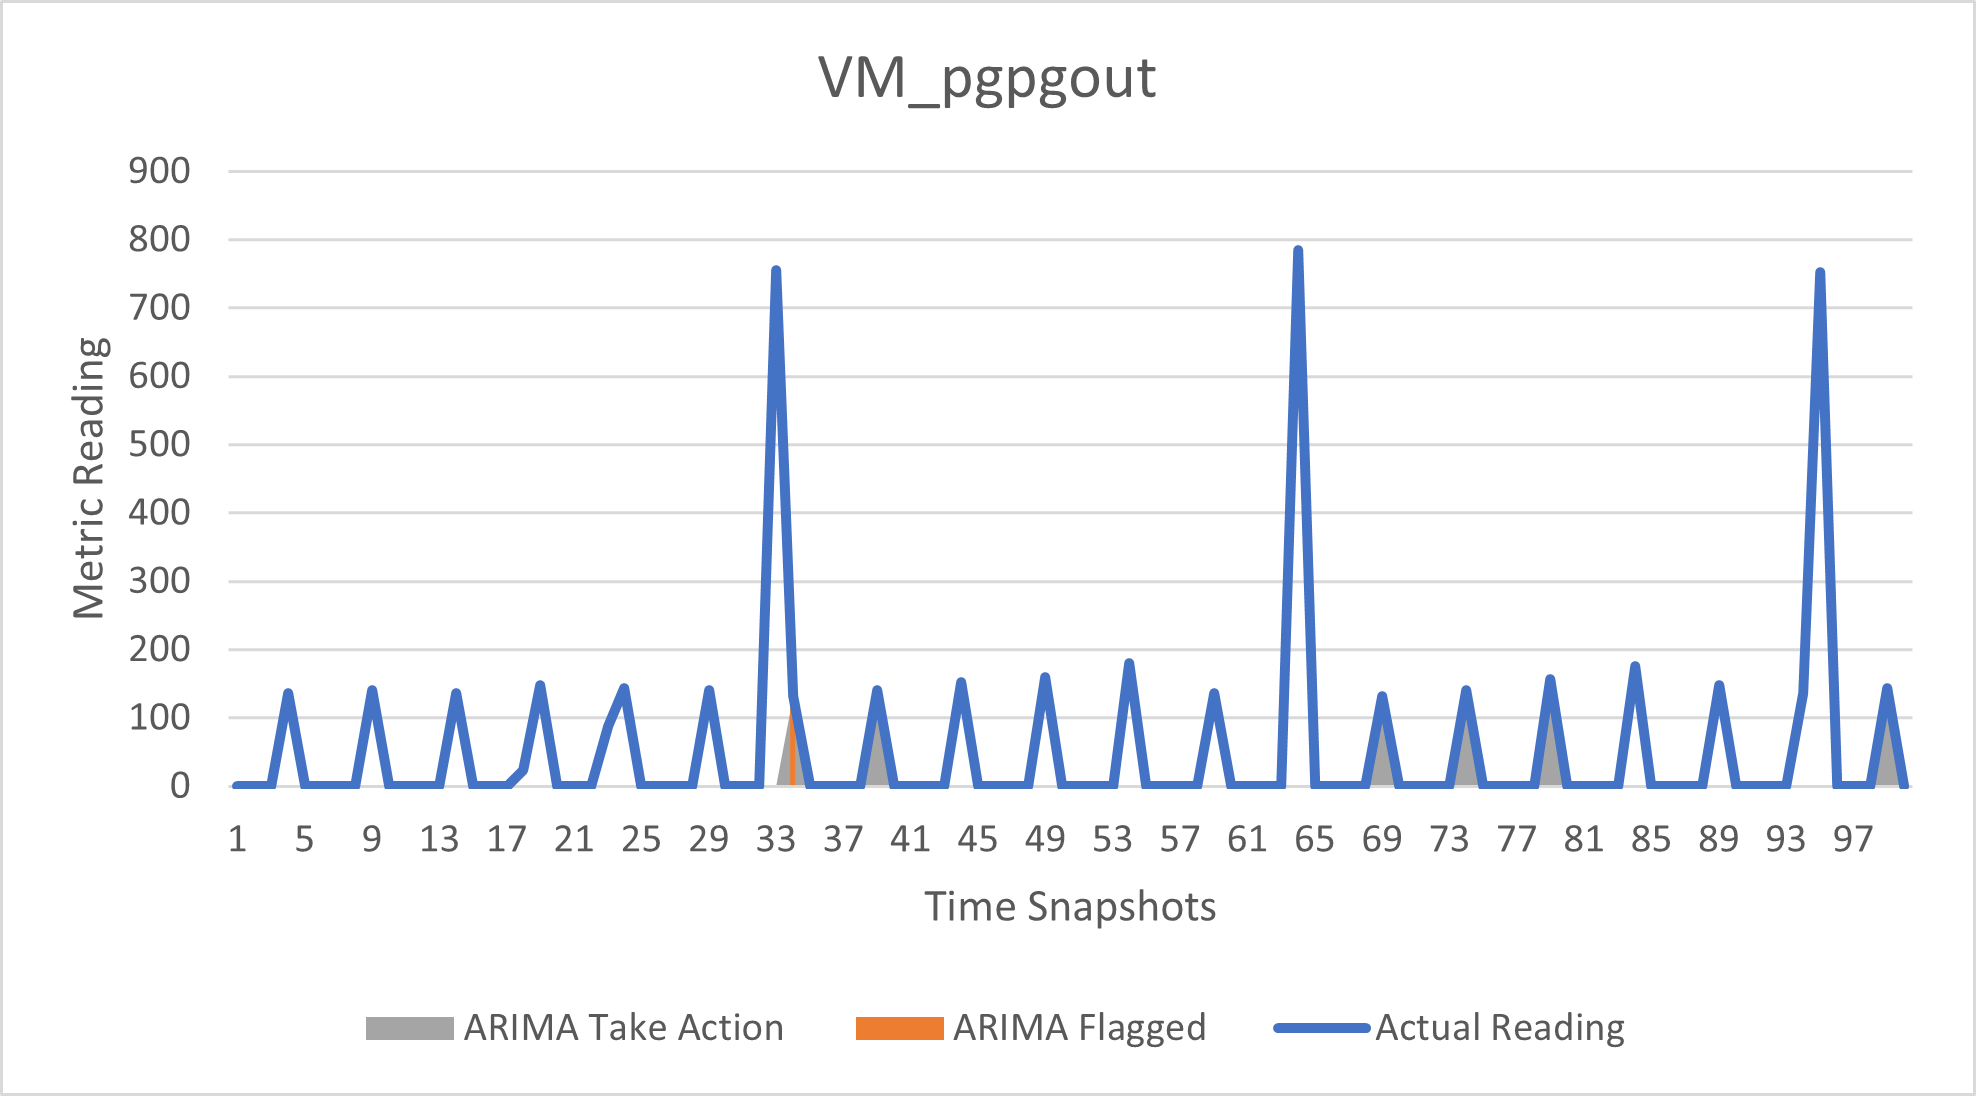
\includegraphics[width=\textwidth]{images/metrics_charts/30_pct_file_load/c1_s1/14.png}
         \caption{VM\_pageout | Adaptive Decision}
         \label{fig:c1_s1_14}
     \end{subfigure}
     \hfill
     \begin{subfigure}[ht]{0.32\textwidth}
         \centering
         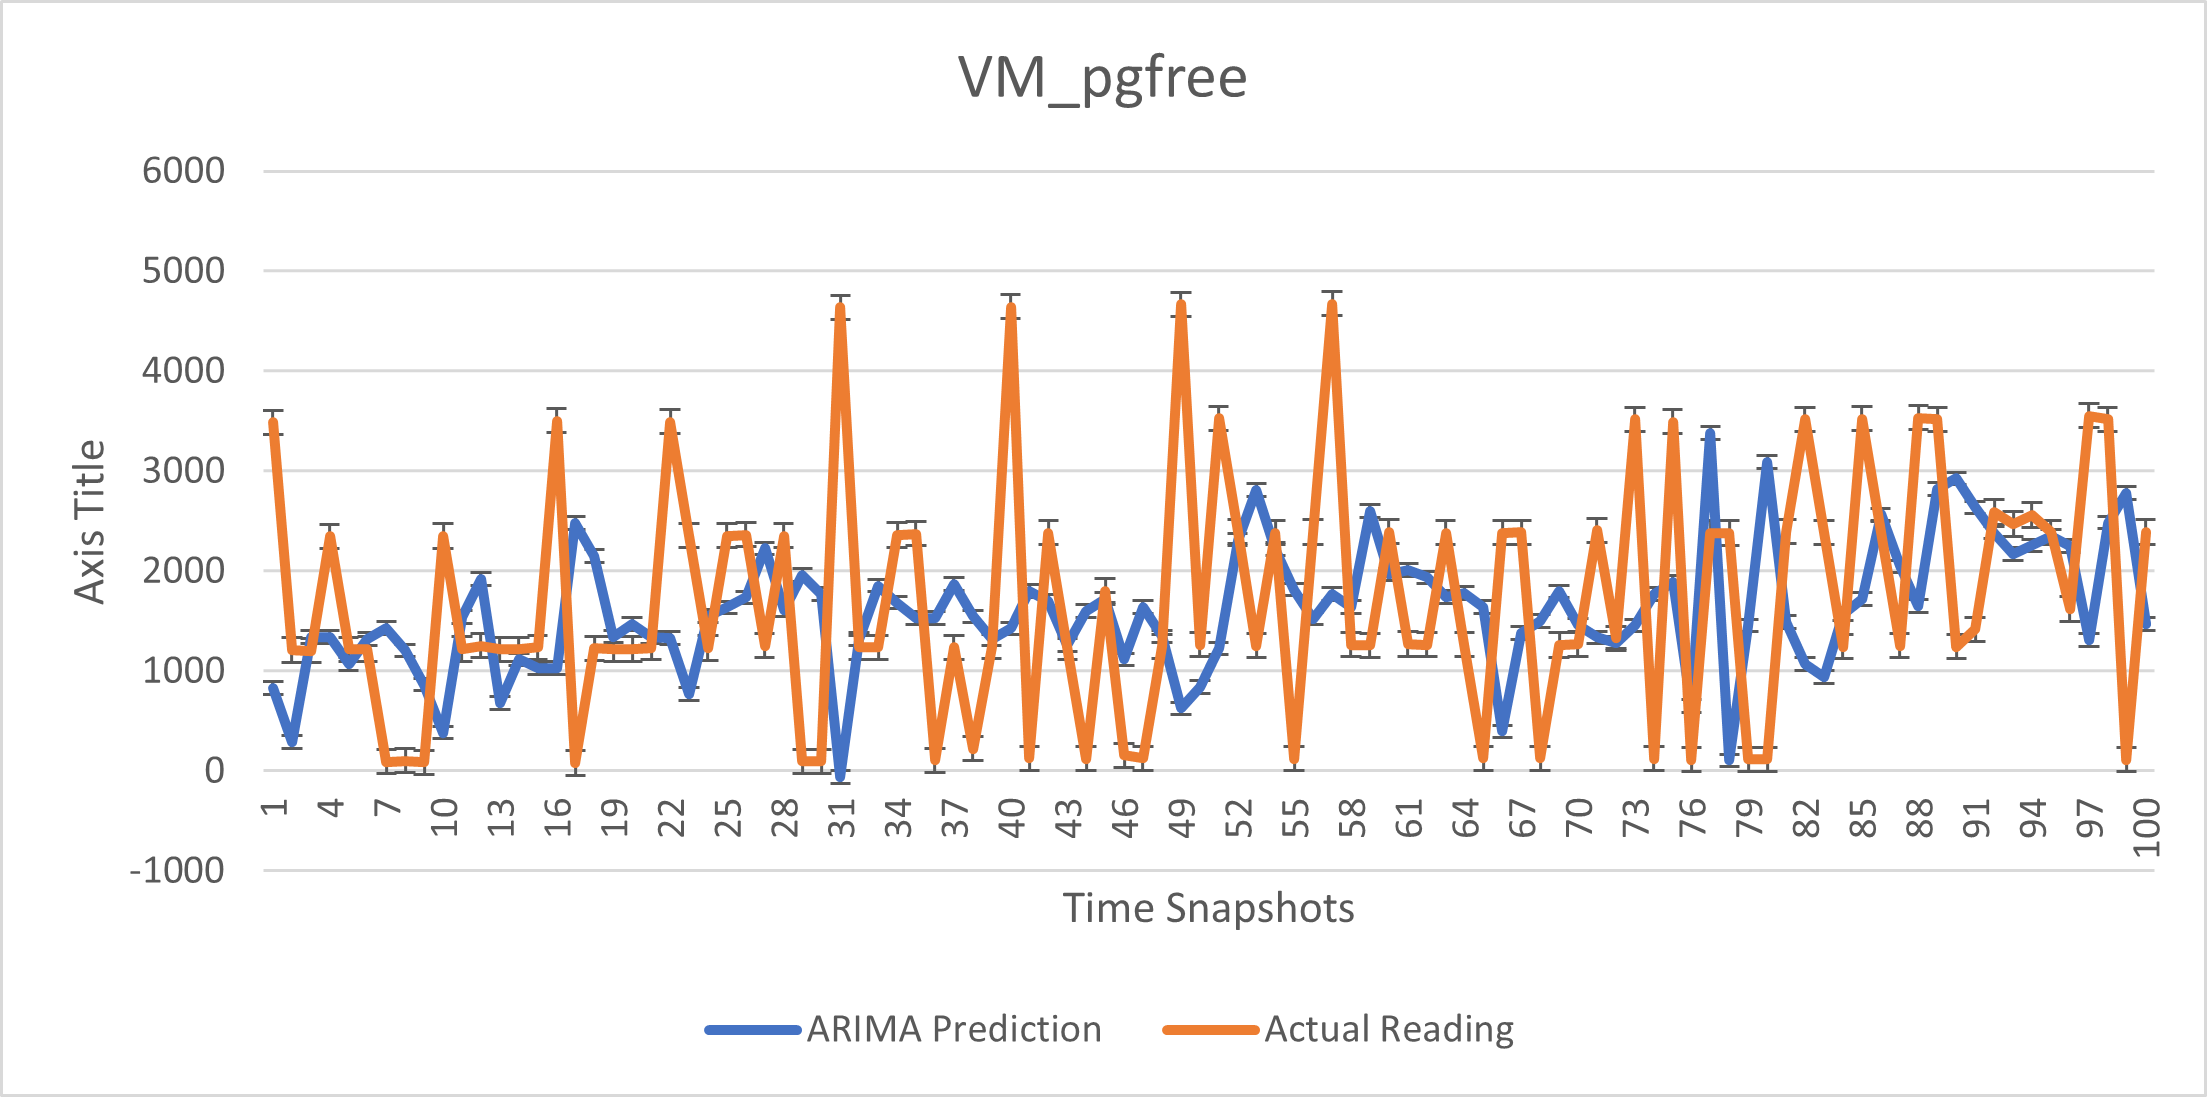
\includegraphics[width=\textwidth]{images/metrics_charts/30_pct_file_load/c1_s1/15.png}
         \caption{VM\_pgfree | ARIMA Prediction}
         \label{fig:c1_s1_15}
     \end{subfigure}
     \hfill
     \begin{subfigure}[ht]{0.32\textwidth}
         \centering
         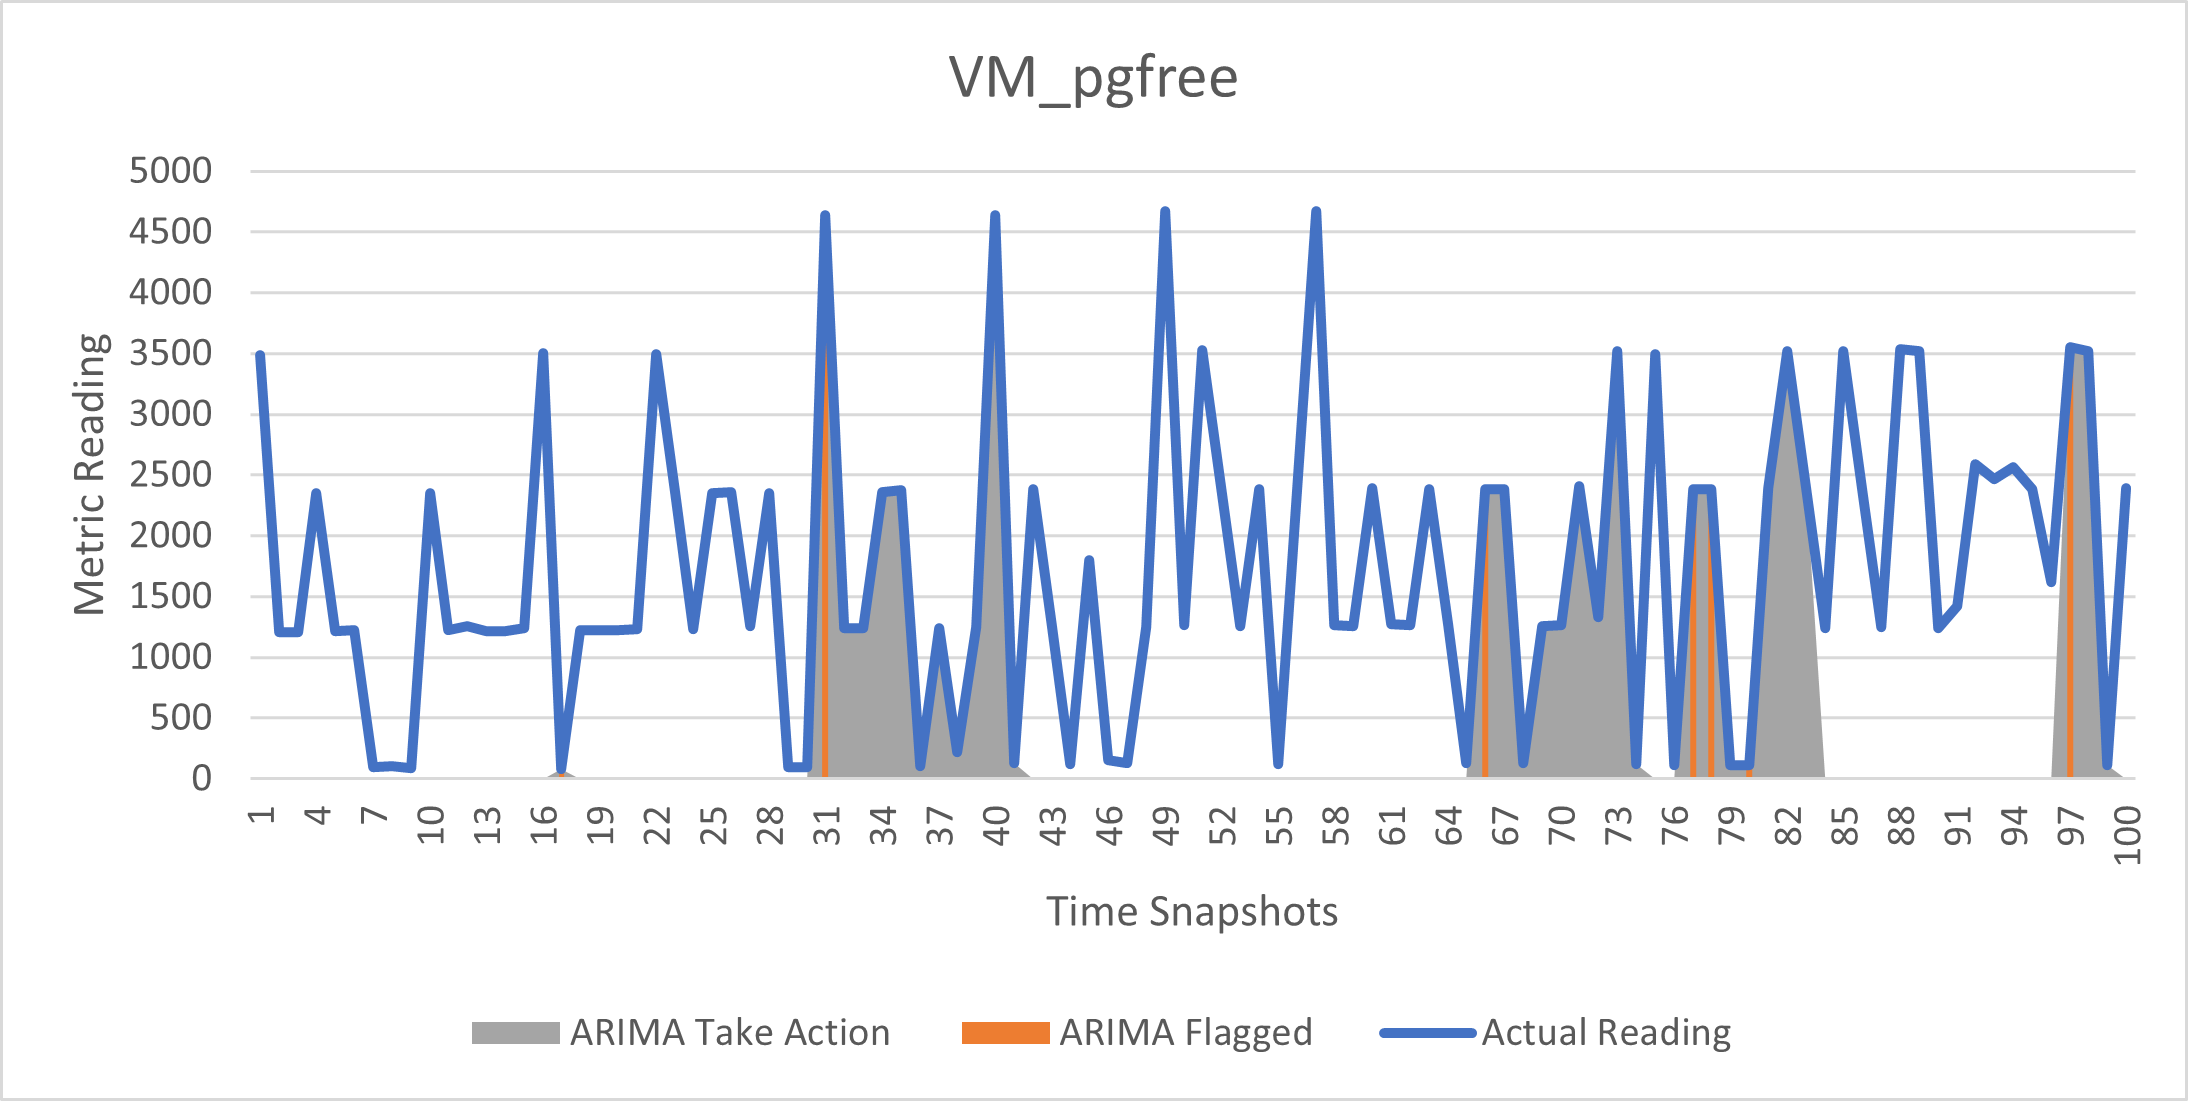
\includegraphics[width=\textwidth]{images/metrics_charts/30_pct_file_load/c1_s1/16.png}
         \caption{VM\_pgfree | Adaptive Decision}
         \label{fig:c1_s1_16}
     \end{subfigure}
     \hfill
     \begin{subfigure}[ht]{0.49\textwidth}
         \centering
         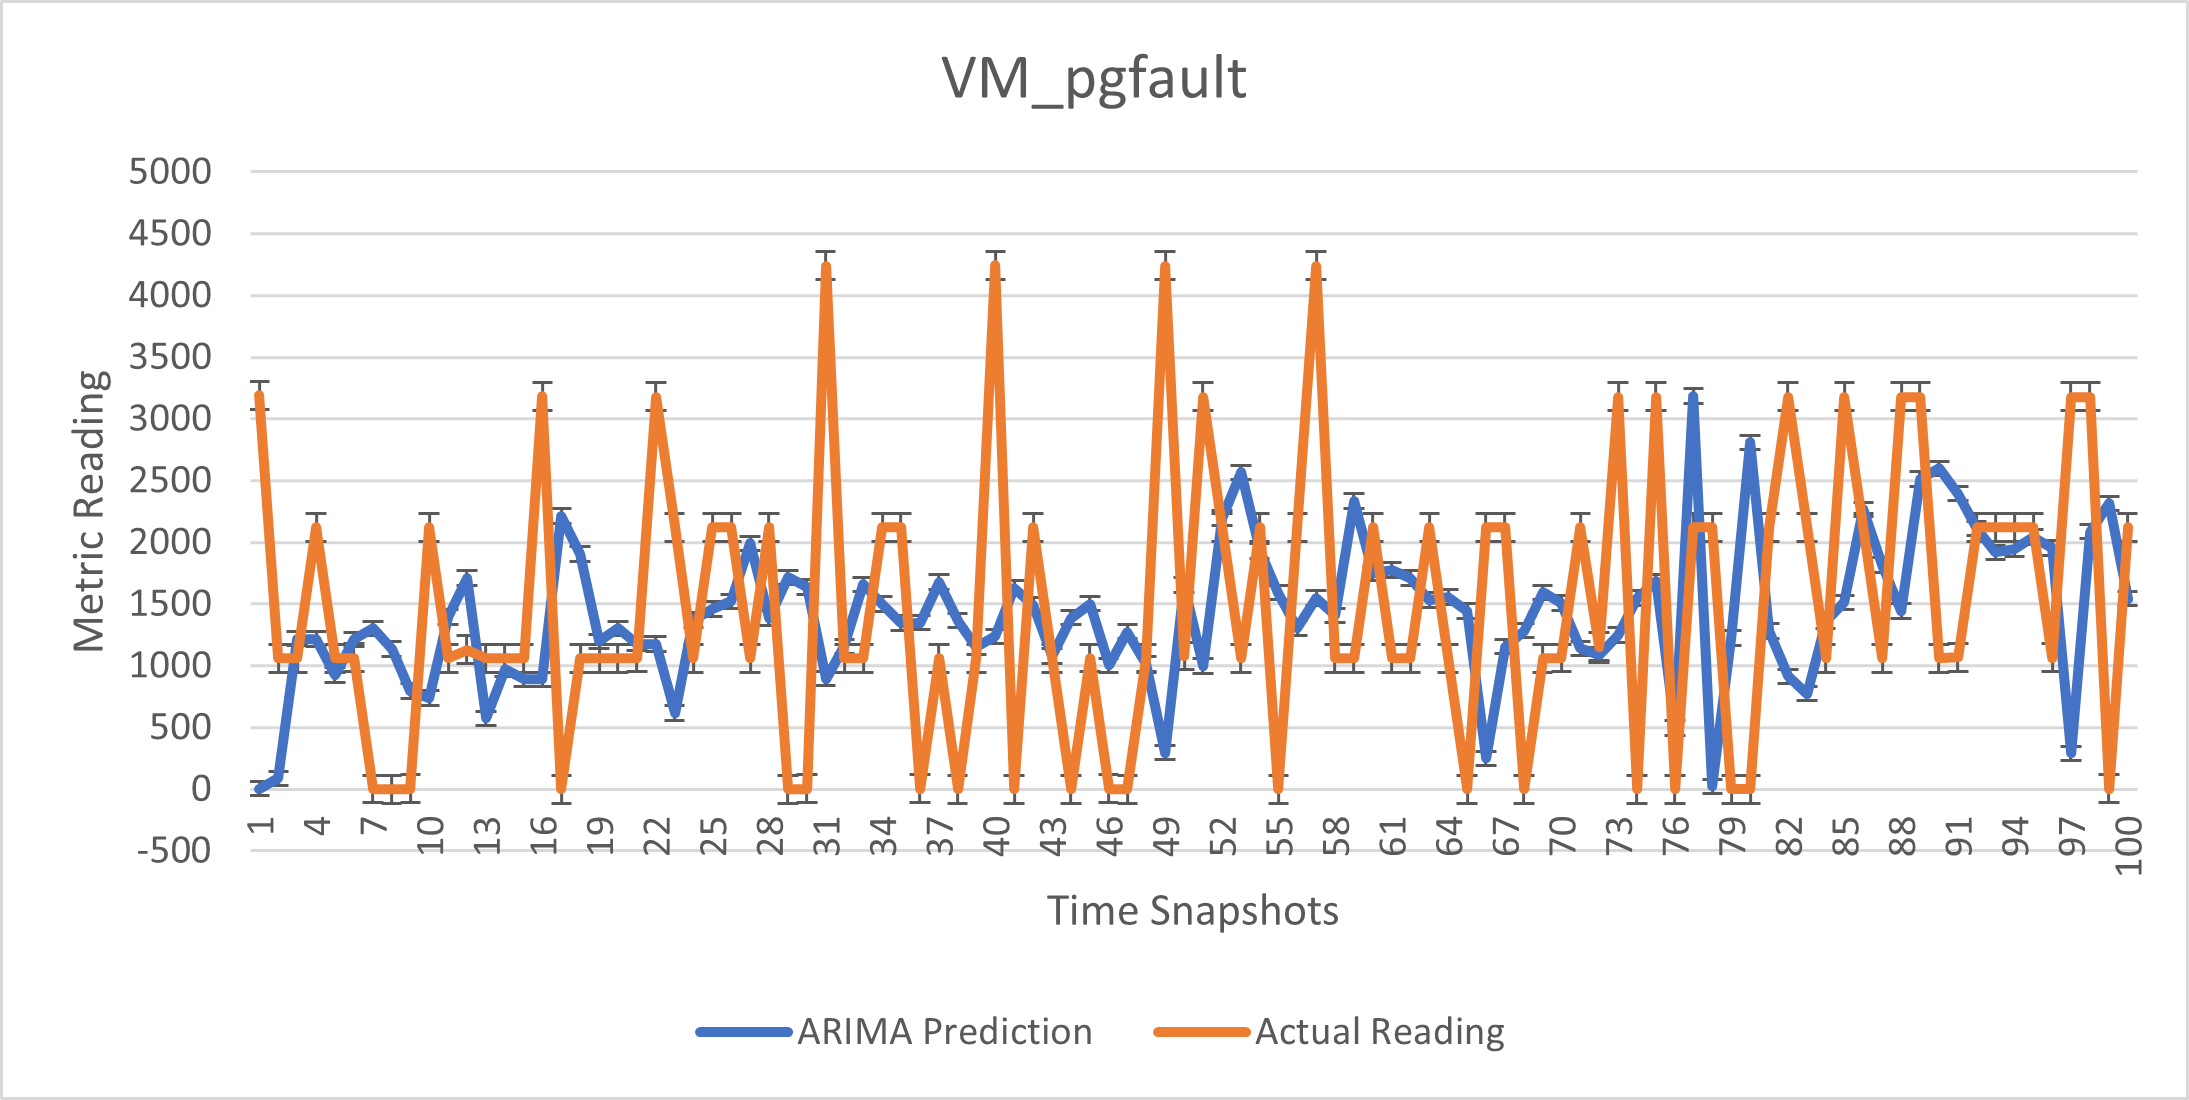
\includegraphics[width=\textwidth]{images/metrics_charts/30_pct_file_load/c1_s1/17.png}
         \caption{VM\_pgfault | ARIMA Prediction}
         \label{fig:c1_s1_17}
     \end{subfigure}
     \hfill
     \begin{subfigure}[ht]{0.49\textwidth}
         \centering
         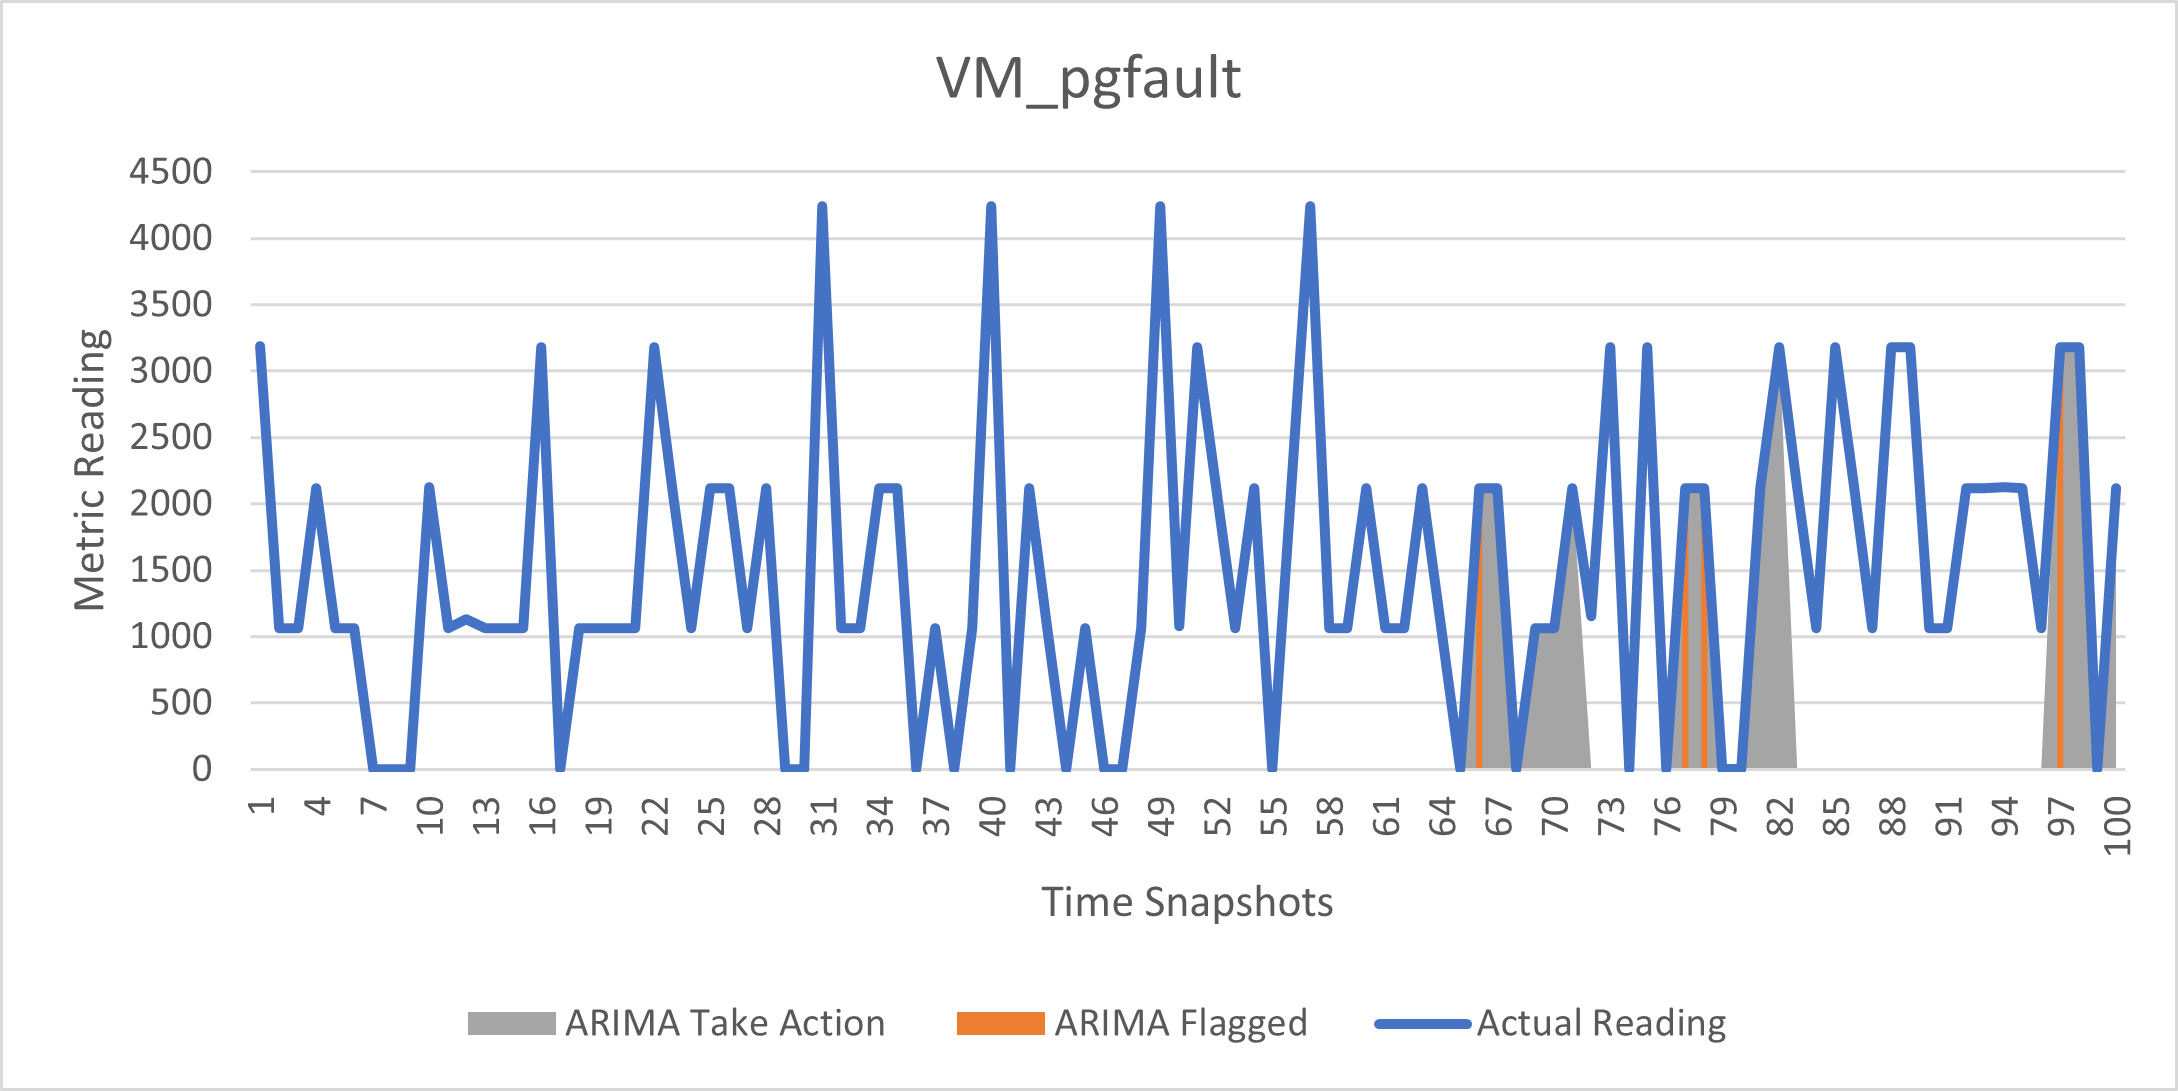
\includegraphics[width=\textwidth]{images/metrics_charts/30_pct_file_load/c1_s1/18.png}
         \caption{VM\_pgfault | Adaptive Decision}
         \label{fig:c1_s1_18}
     \end{subfigure}
     \hfill
     
     \caption{Memory Metrics | Case Study: 1}
     \label{fig:c1_s1_memory}
\end{figure*}

For disk-related metrics, we had two different partitions: sda and sda5. Figure \ref{fig:c1_s1_disksda} shows the metrics for the sda partition. For DISKBSIZE, we can see that ARIMA had been flagging for a while on the lower spikes and building up the anomaly score enough to trigger an action to be taken in the last quarter of the experiment. For DISKBUSY, however, we noticed the anomaly score was triggered much earlier. Meanwhile, for DISKWRITE and DISKXFER, we can see little to no flagged area. DISKXFER have seen three major spikes, but the distance between them was too big for the anomaly score to reach its threshold. Figure \ref{fig:c1_s1_disksda5} shows the disk-related metrics for partition sda5. In sda5, we see similar properties as seen in sda. However, DISKBUSY for sda5 broke its trend much earlier than sda; therefore, we could see it got flagged much earlier as well.

\begin{figure*}[tbp]
     \centering
     \begin{subfigure}[ht]{0.32\textwidth}
         \centering
         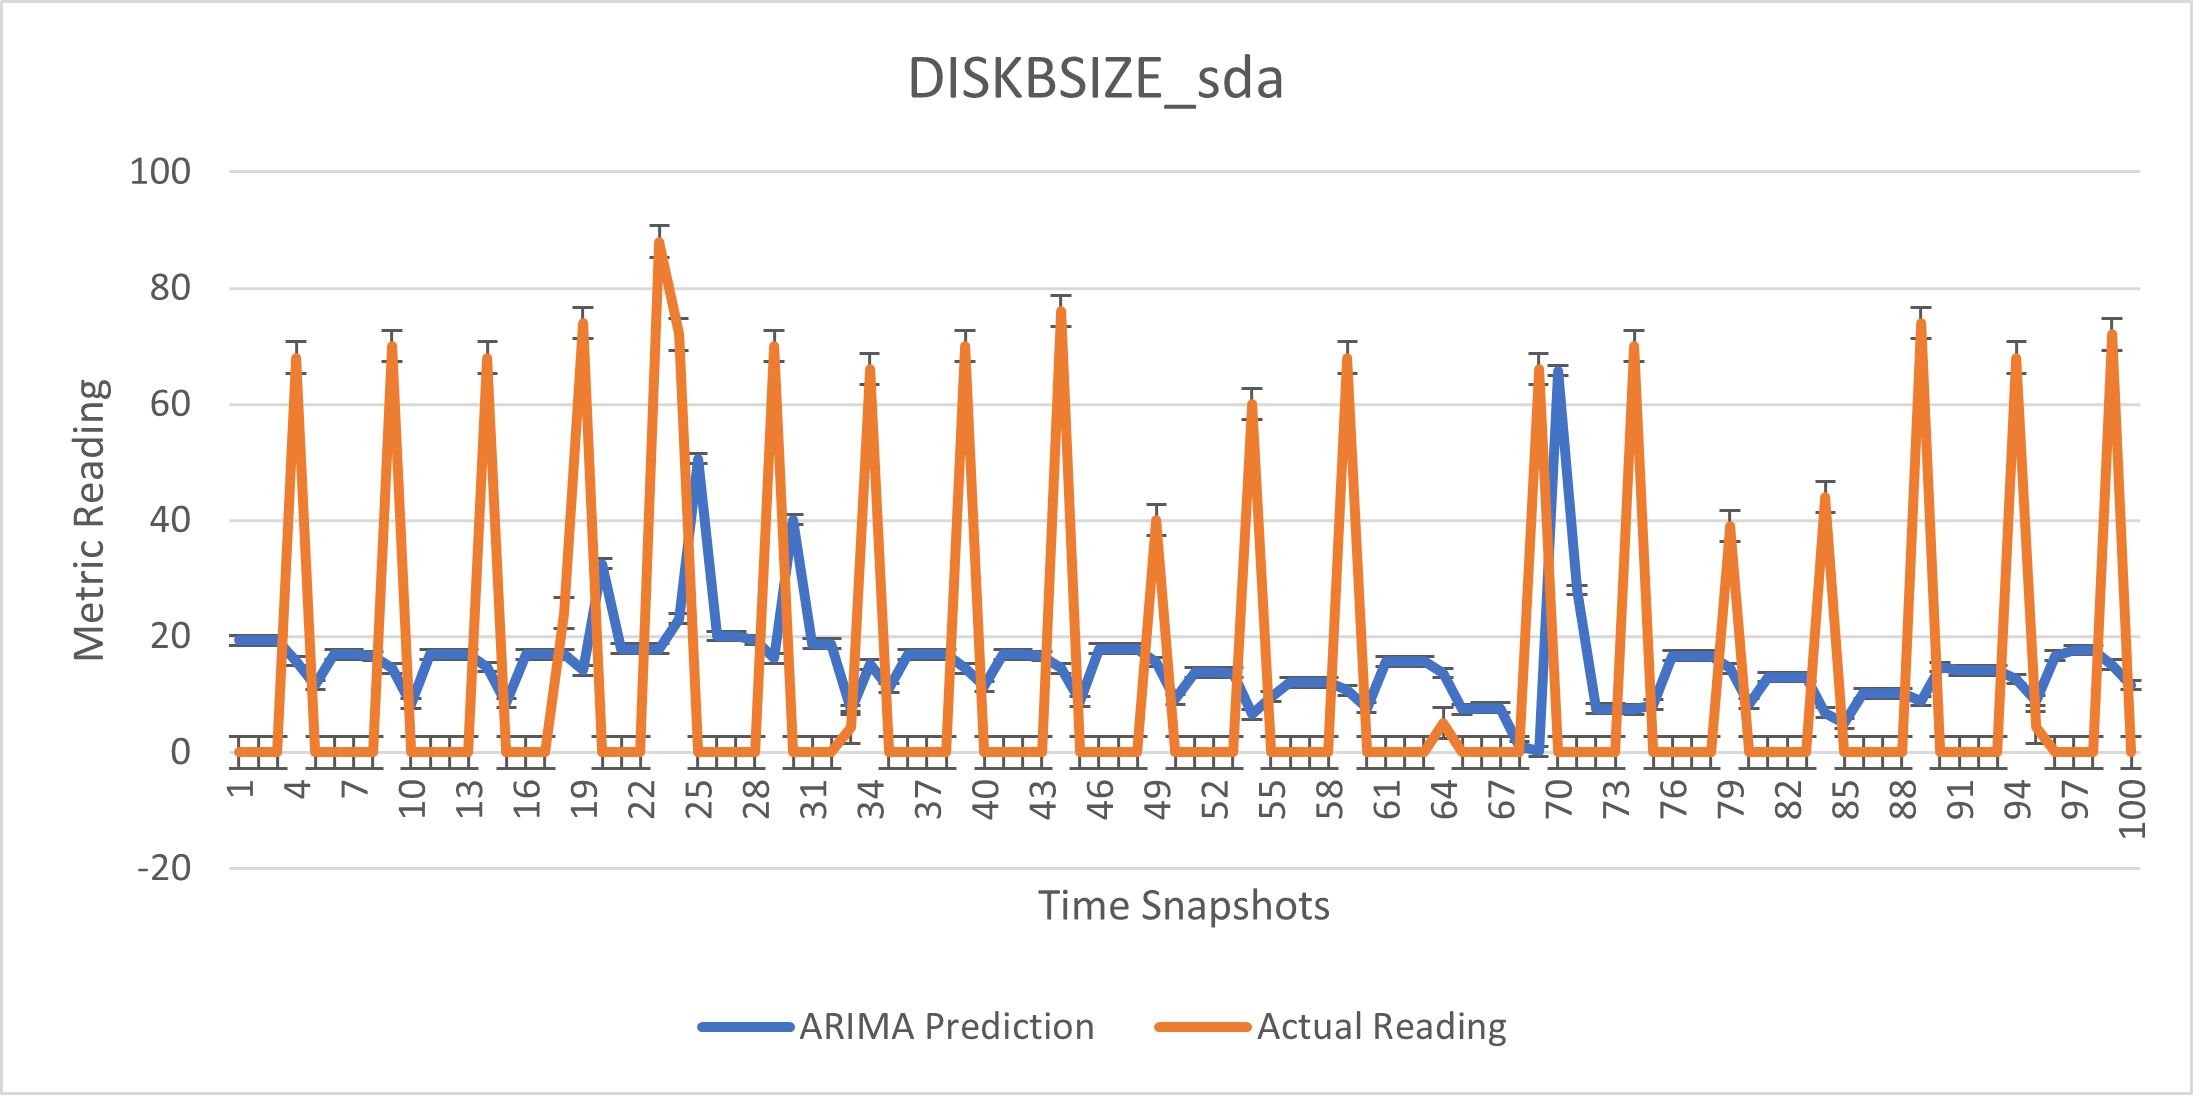
\includegraphics[width=\textwidth]{images/metrics_charts/30_pct_file_load/c1_s1/19.png}
         \caption{DISKBSIZE\_sda | ARIMA Prediction}
         \label{fig:c1_s1_19}
     \end{subfigure}
     \hfill
     \begin{subfigure}[ht]{0.32\textwidth}
         \centering
         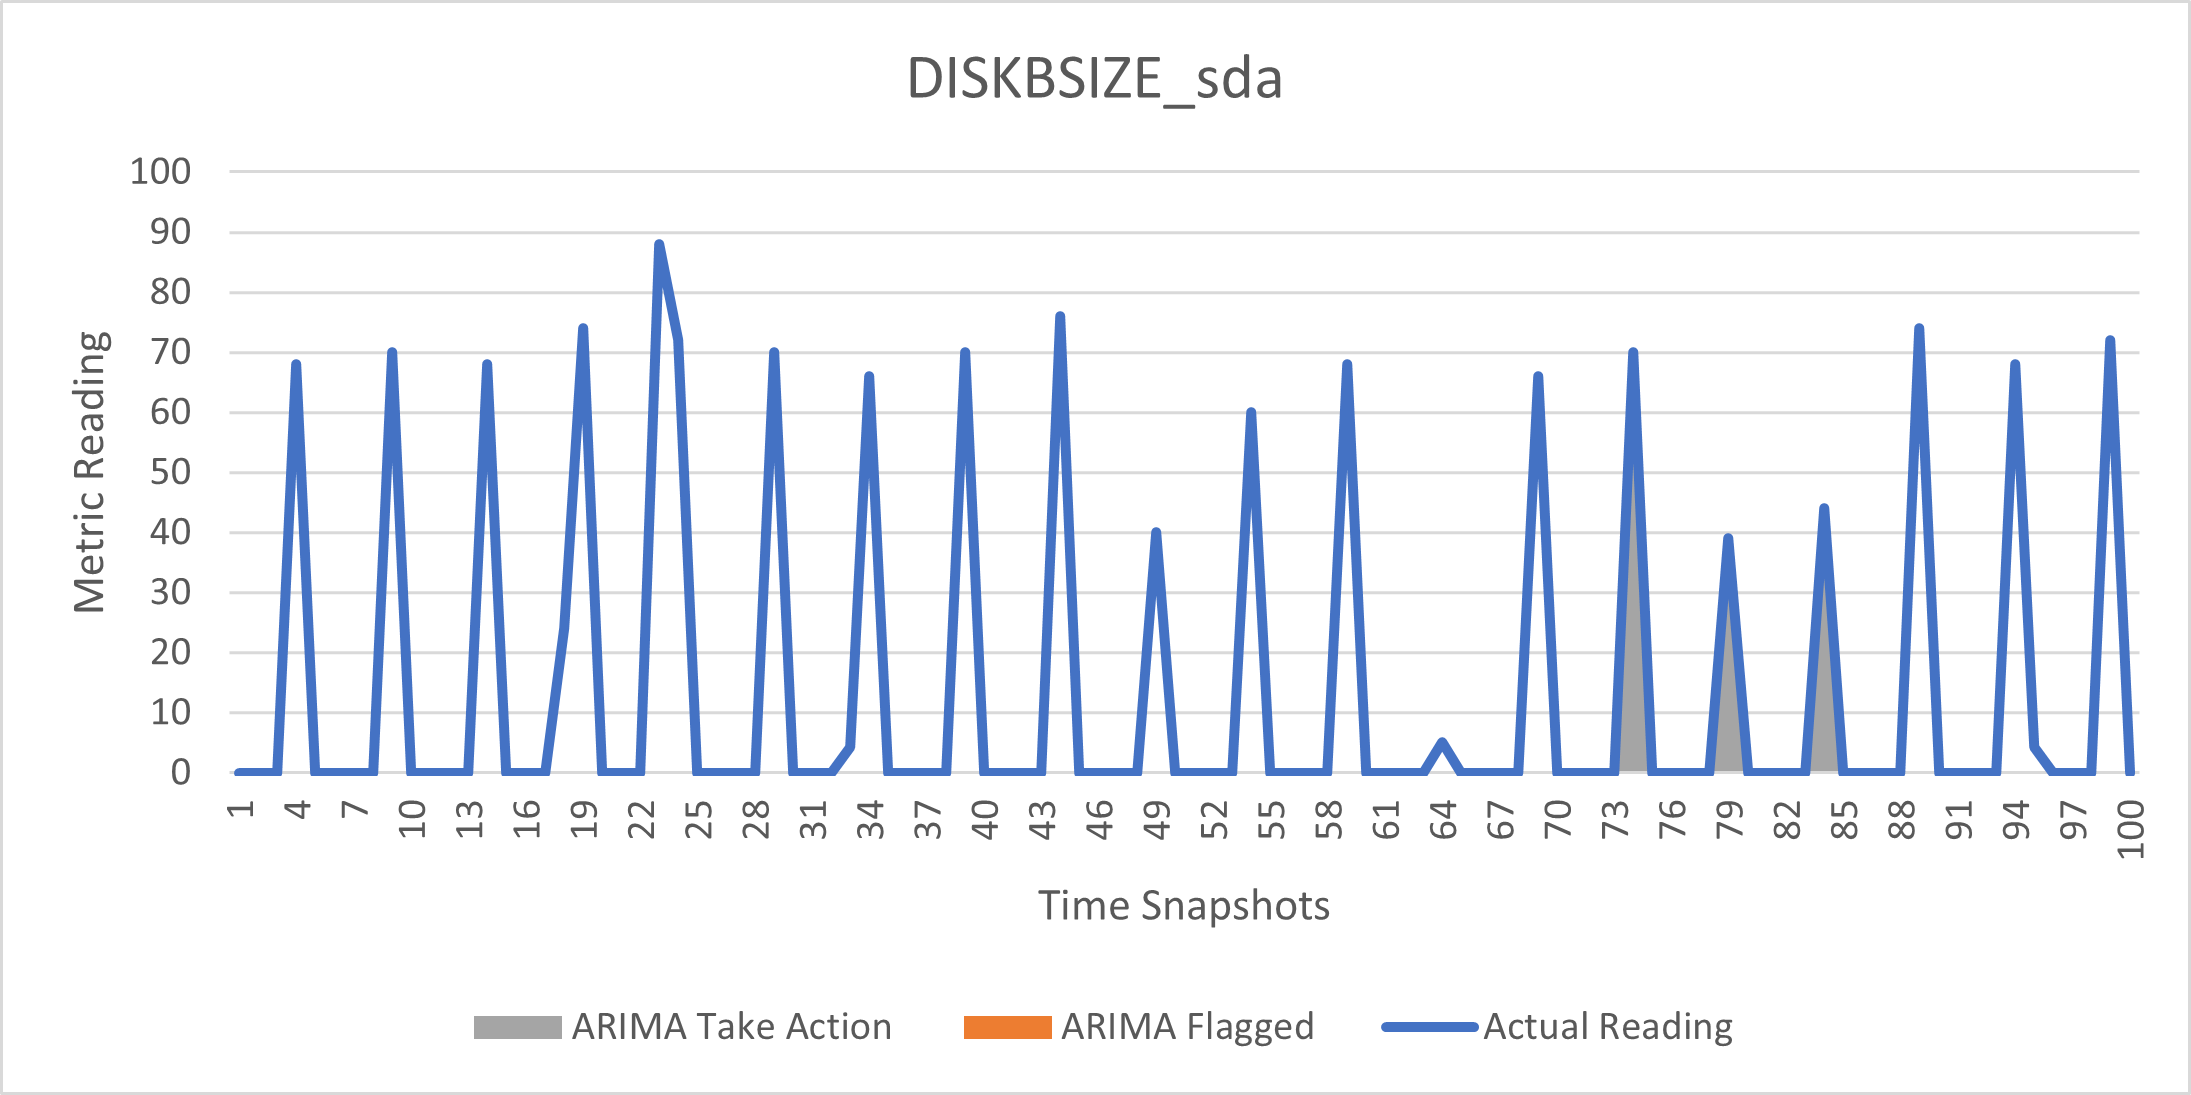
\includegraphics[width=\textwidth]{images/metrics_charts/30_pct_file_load/c1_s1/20.png}
         \caption{DISKBSIZE\_sda | Adaptive Decision}
         \label{fig:c1_s1_20}
     \end{subfigure}
     \hfill
     \begin{subfigure}[ht]{0.32\textwidth}
         \centering
         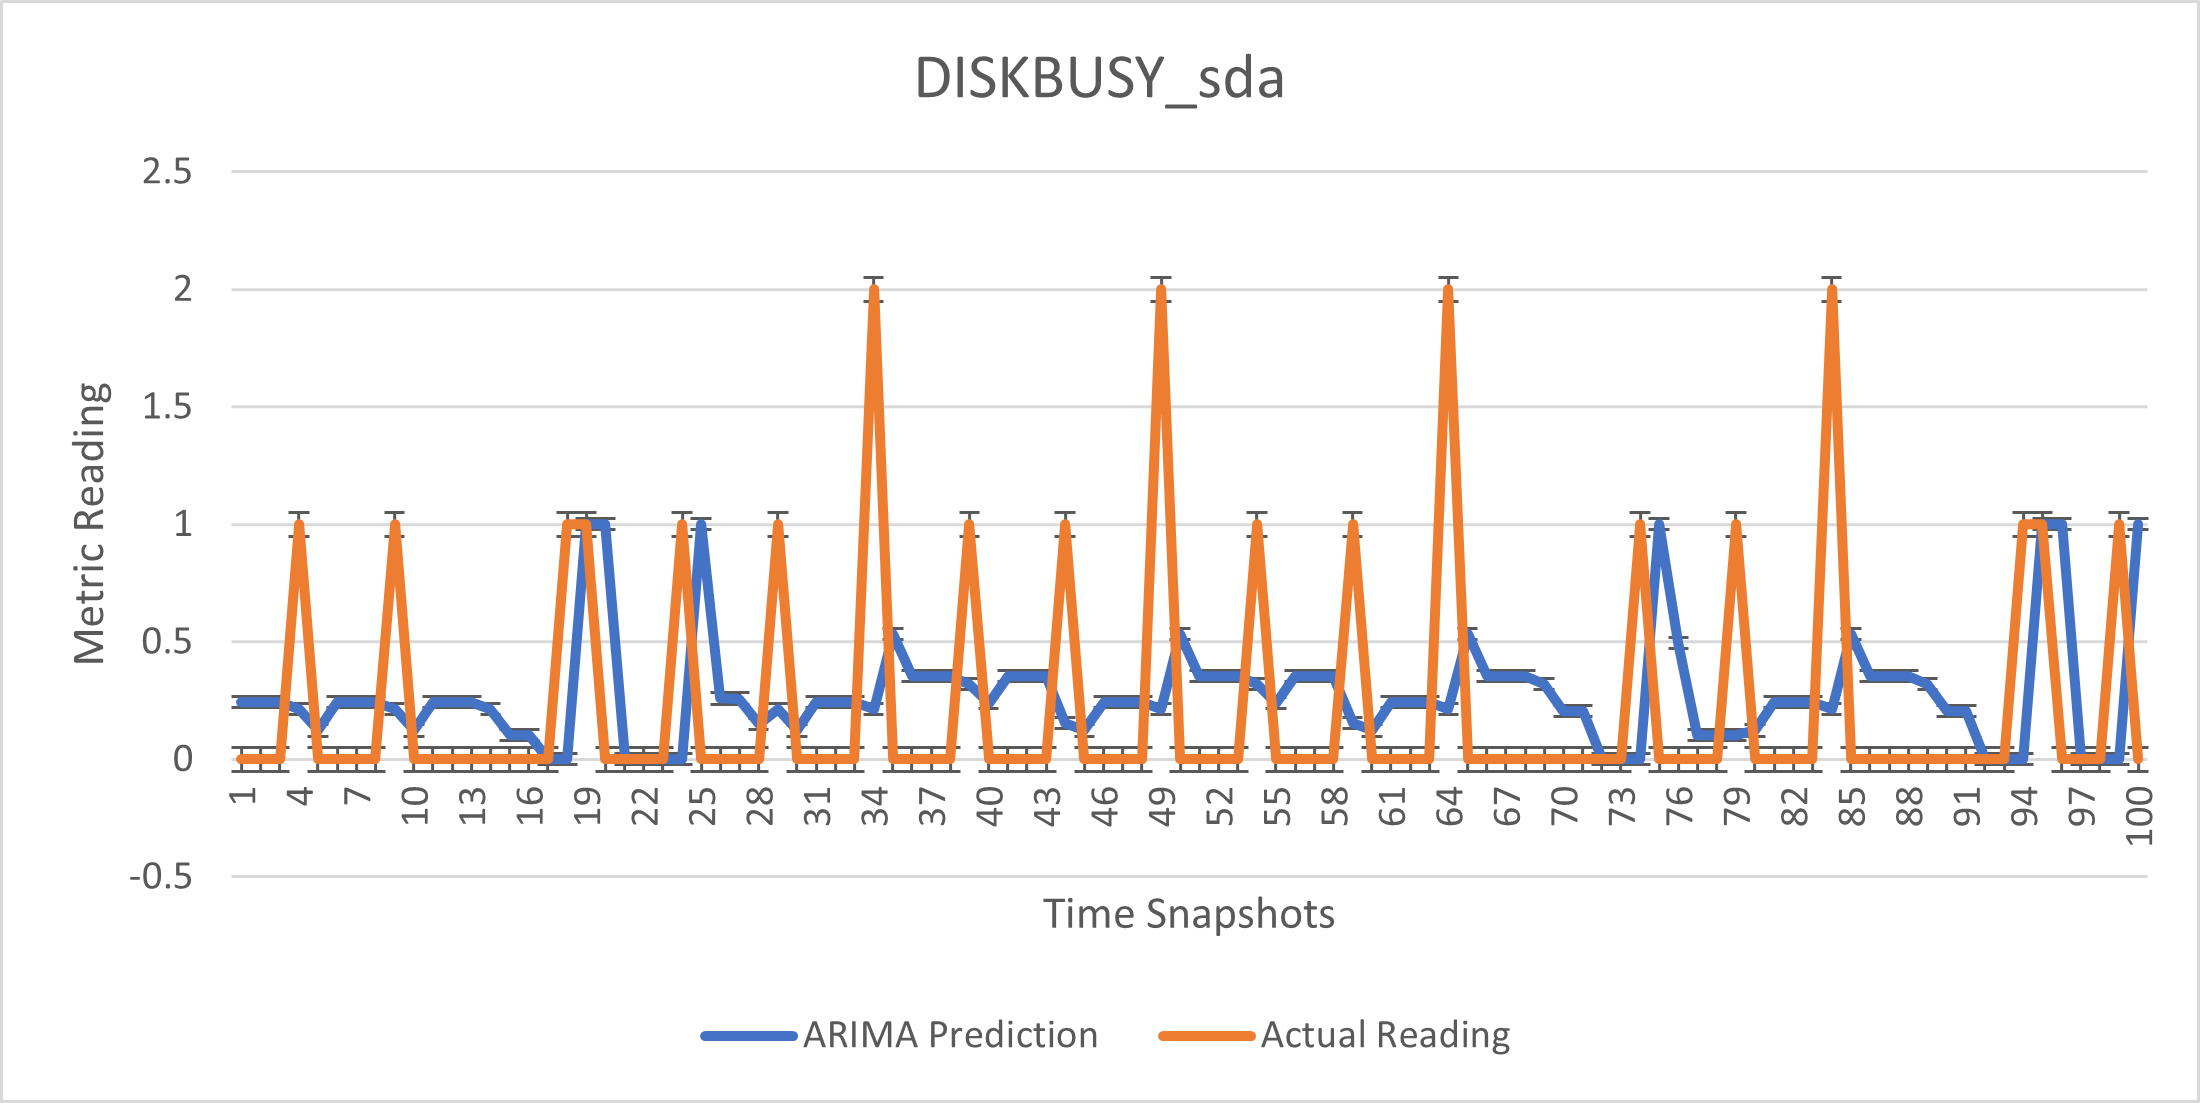
\includegraphics[width=\textwidth]{images/metrics_charts/30_pct_file_load/c1_s1/23.png}
         \caption{DISKBUSY\_sda | ARIMA Prediction}
         \label{fig:c1_s1_23}
     \end{subfigure}
     \hfill
     \begin{subfigure}[ht]{0.32\textwidth}
         \centering
         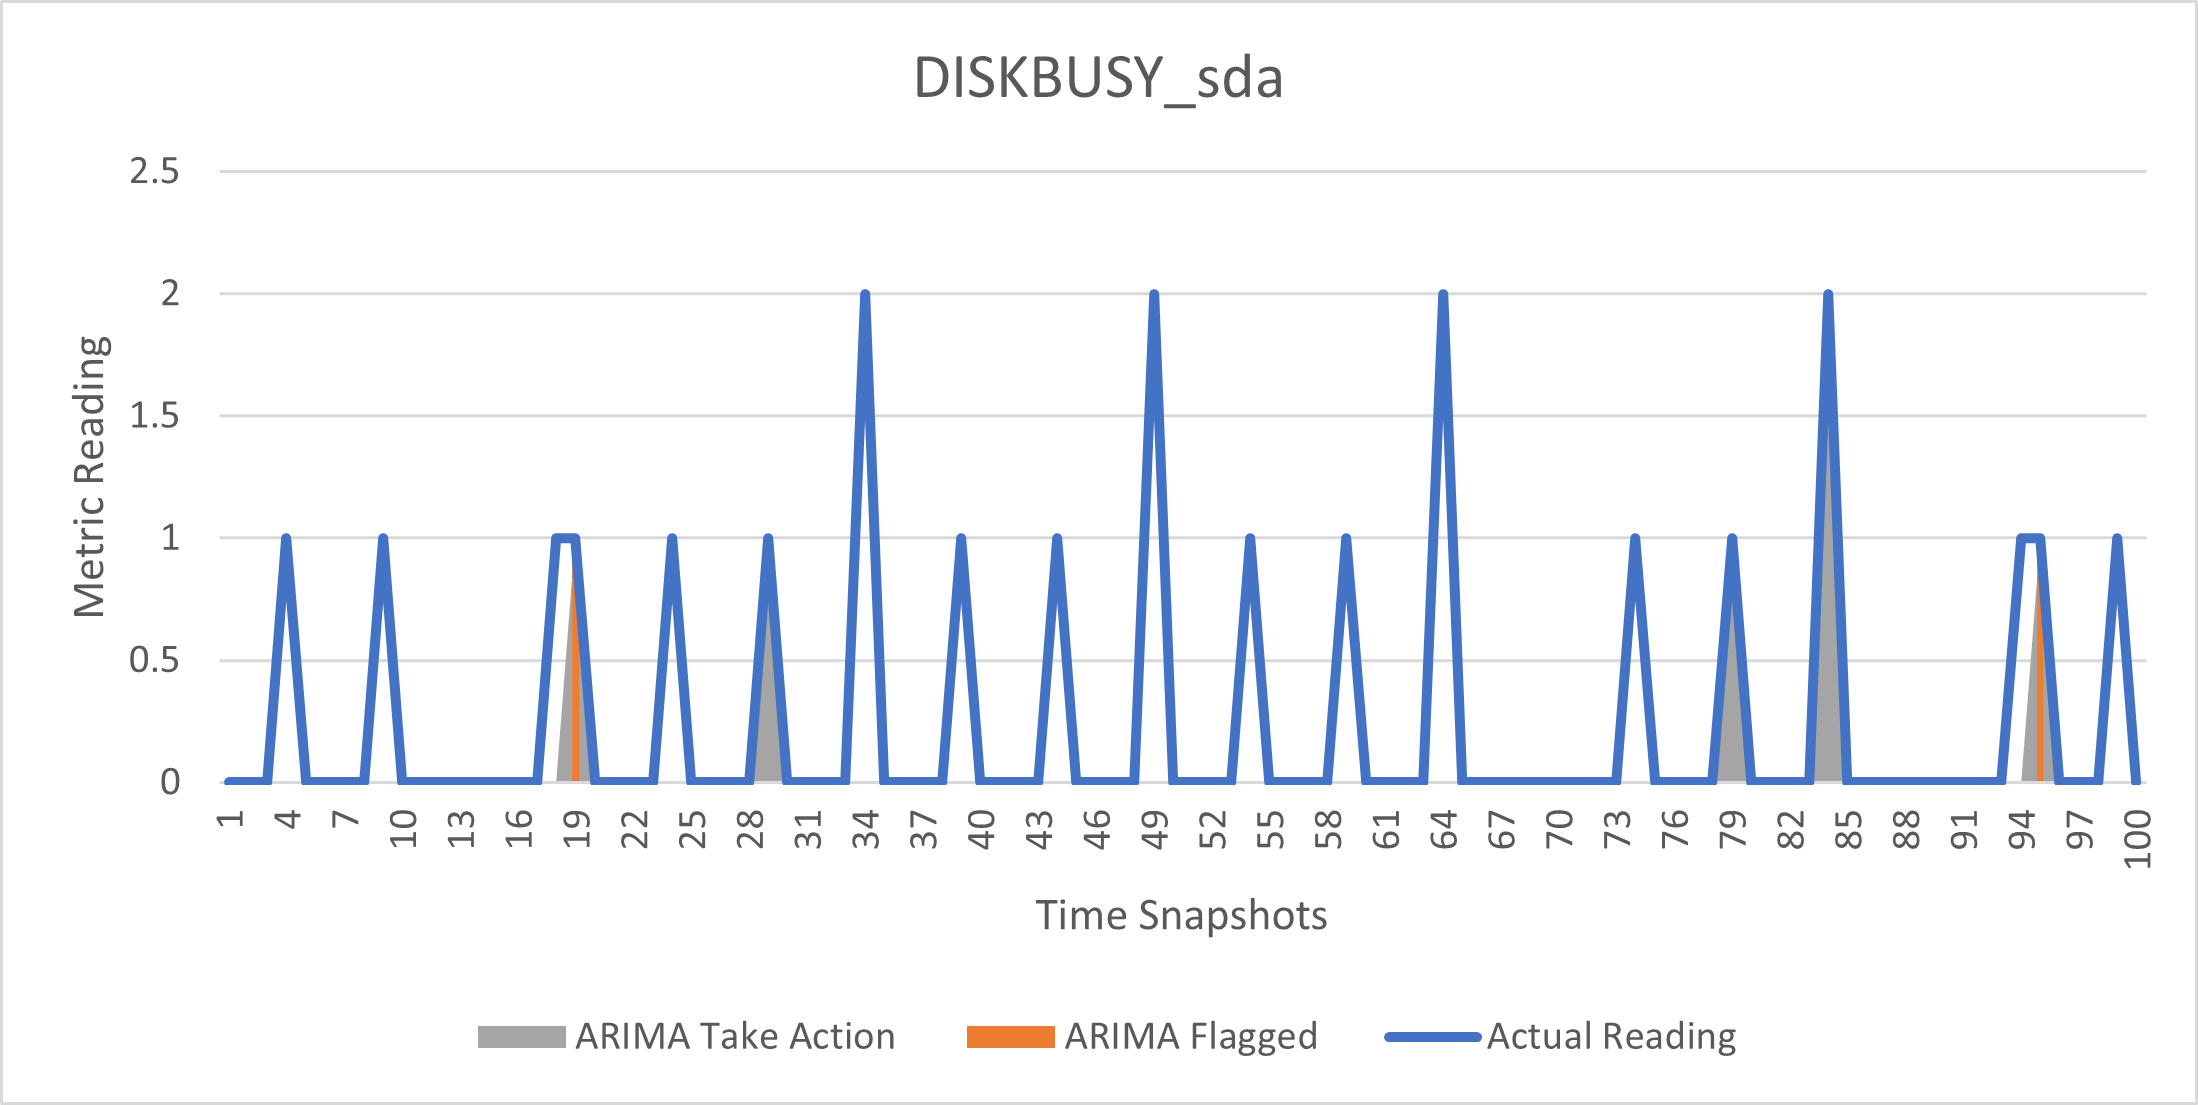
\includegraphics[width=\textwidth]{images/metrics_charts/30_pct_file_load/c1_s1/24.png}
         \caption{DISKBUSY\_sda | Adaptive Decision}
         \label{fig:c1_s1_24}
     \end{subfigure}
     \hfill
     \begin{subfigure}[ht]{0.32\textwidth}
         \centering
         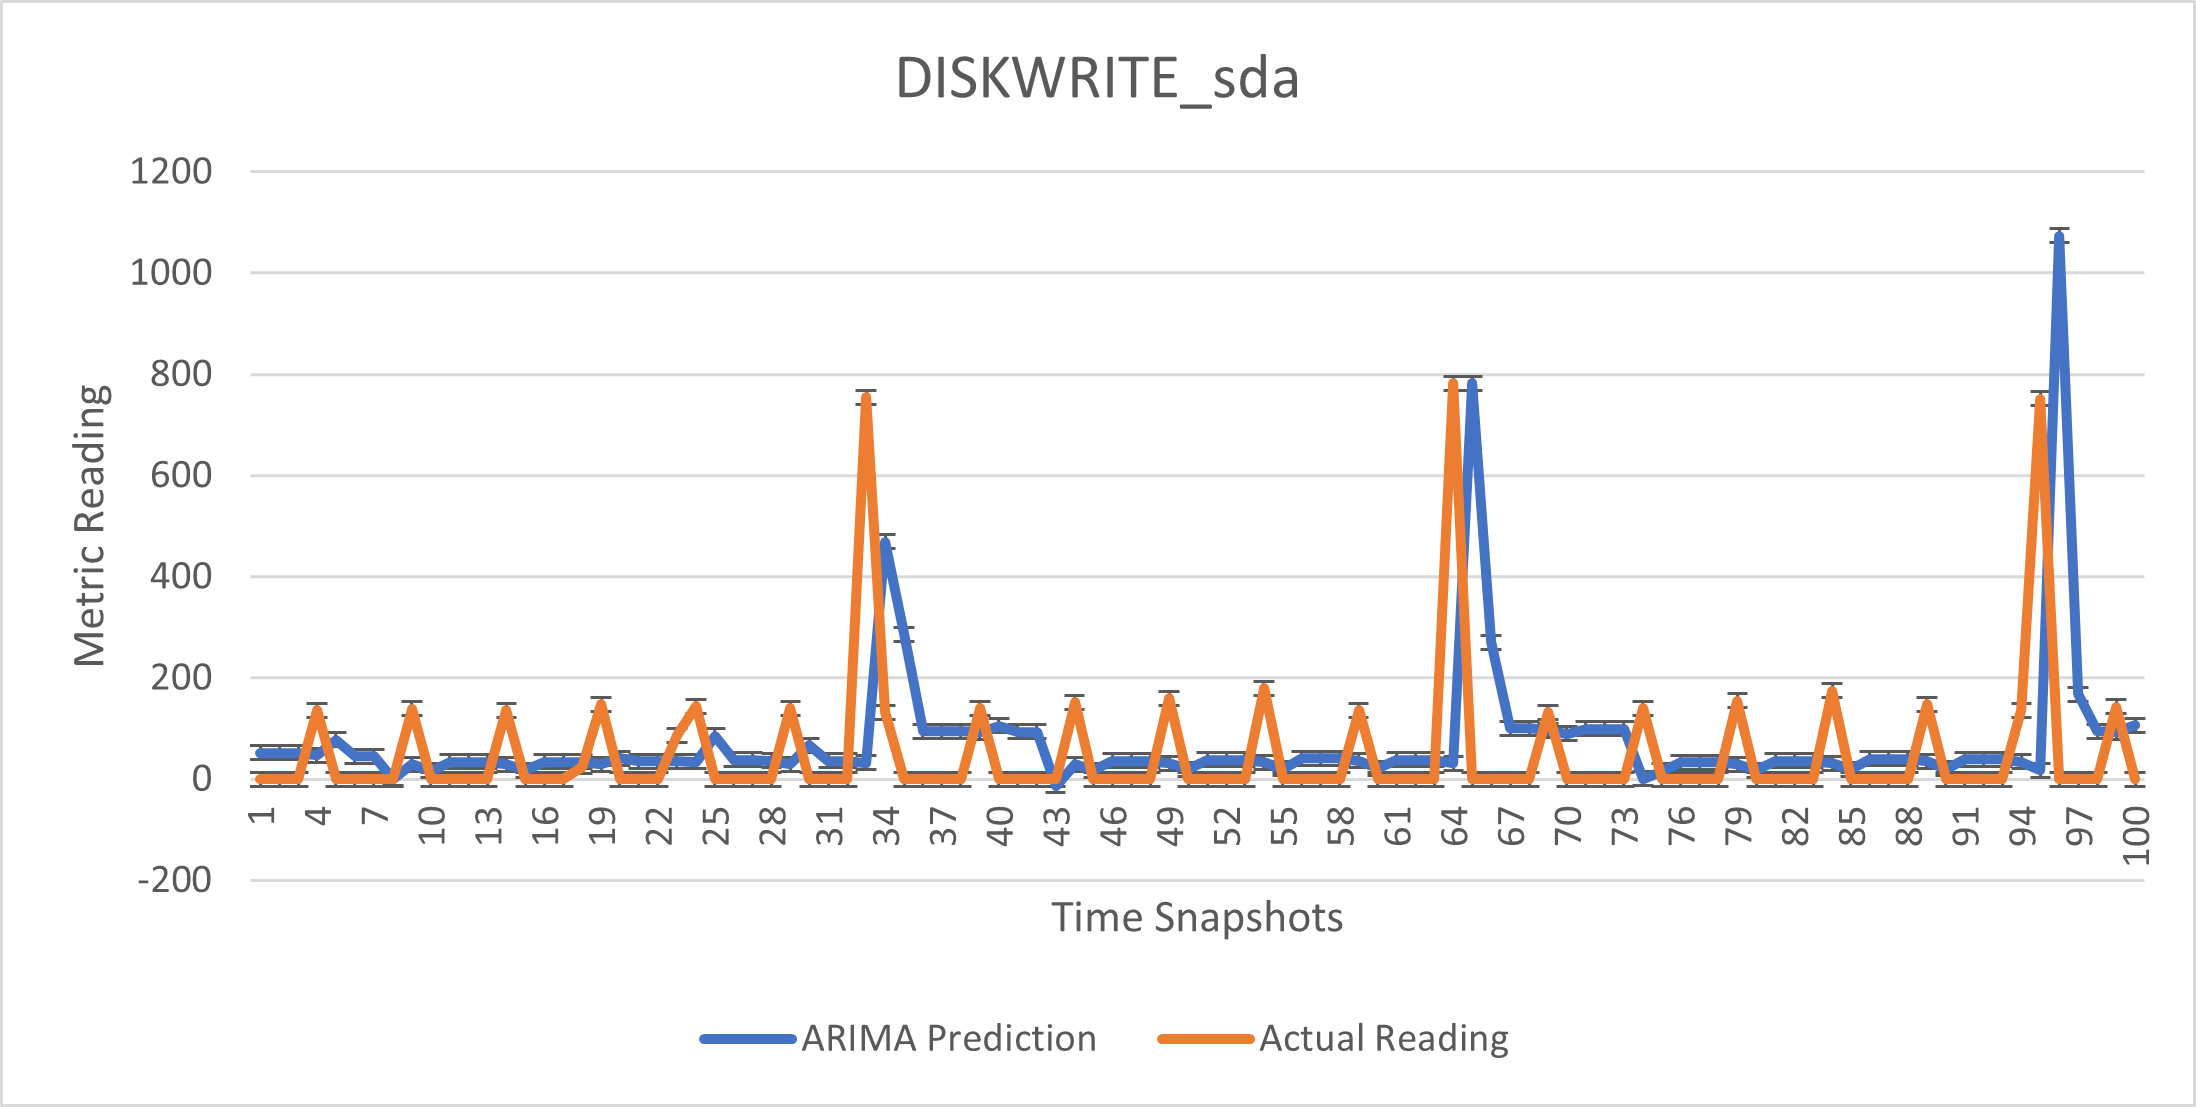
\includegraphics[width=\textwidth]{images/metrics_charts/30_pct_file_load/c1_s1/27.png}
         \caption{DISKWRITE\_sda | ARIMA Prediction}
         \label{fig:c1_s1_27}
     \end{subfigure}
     \hfill
     \begin{subfigure}[ht]{0.32\textwidth}
         \centering
         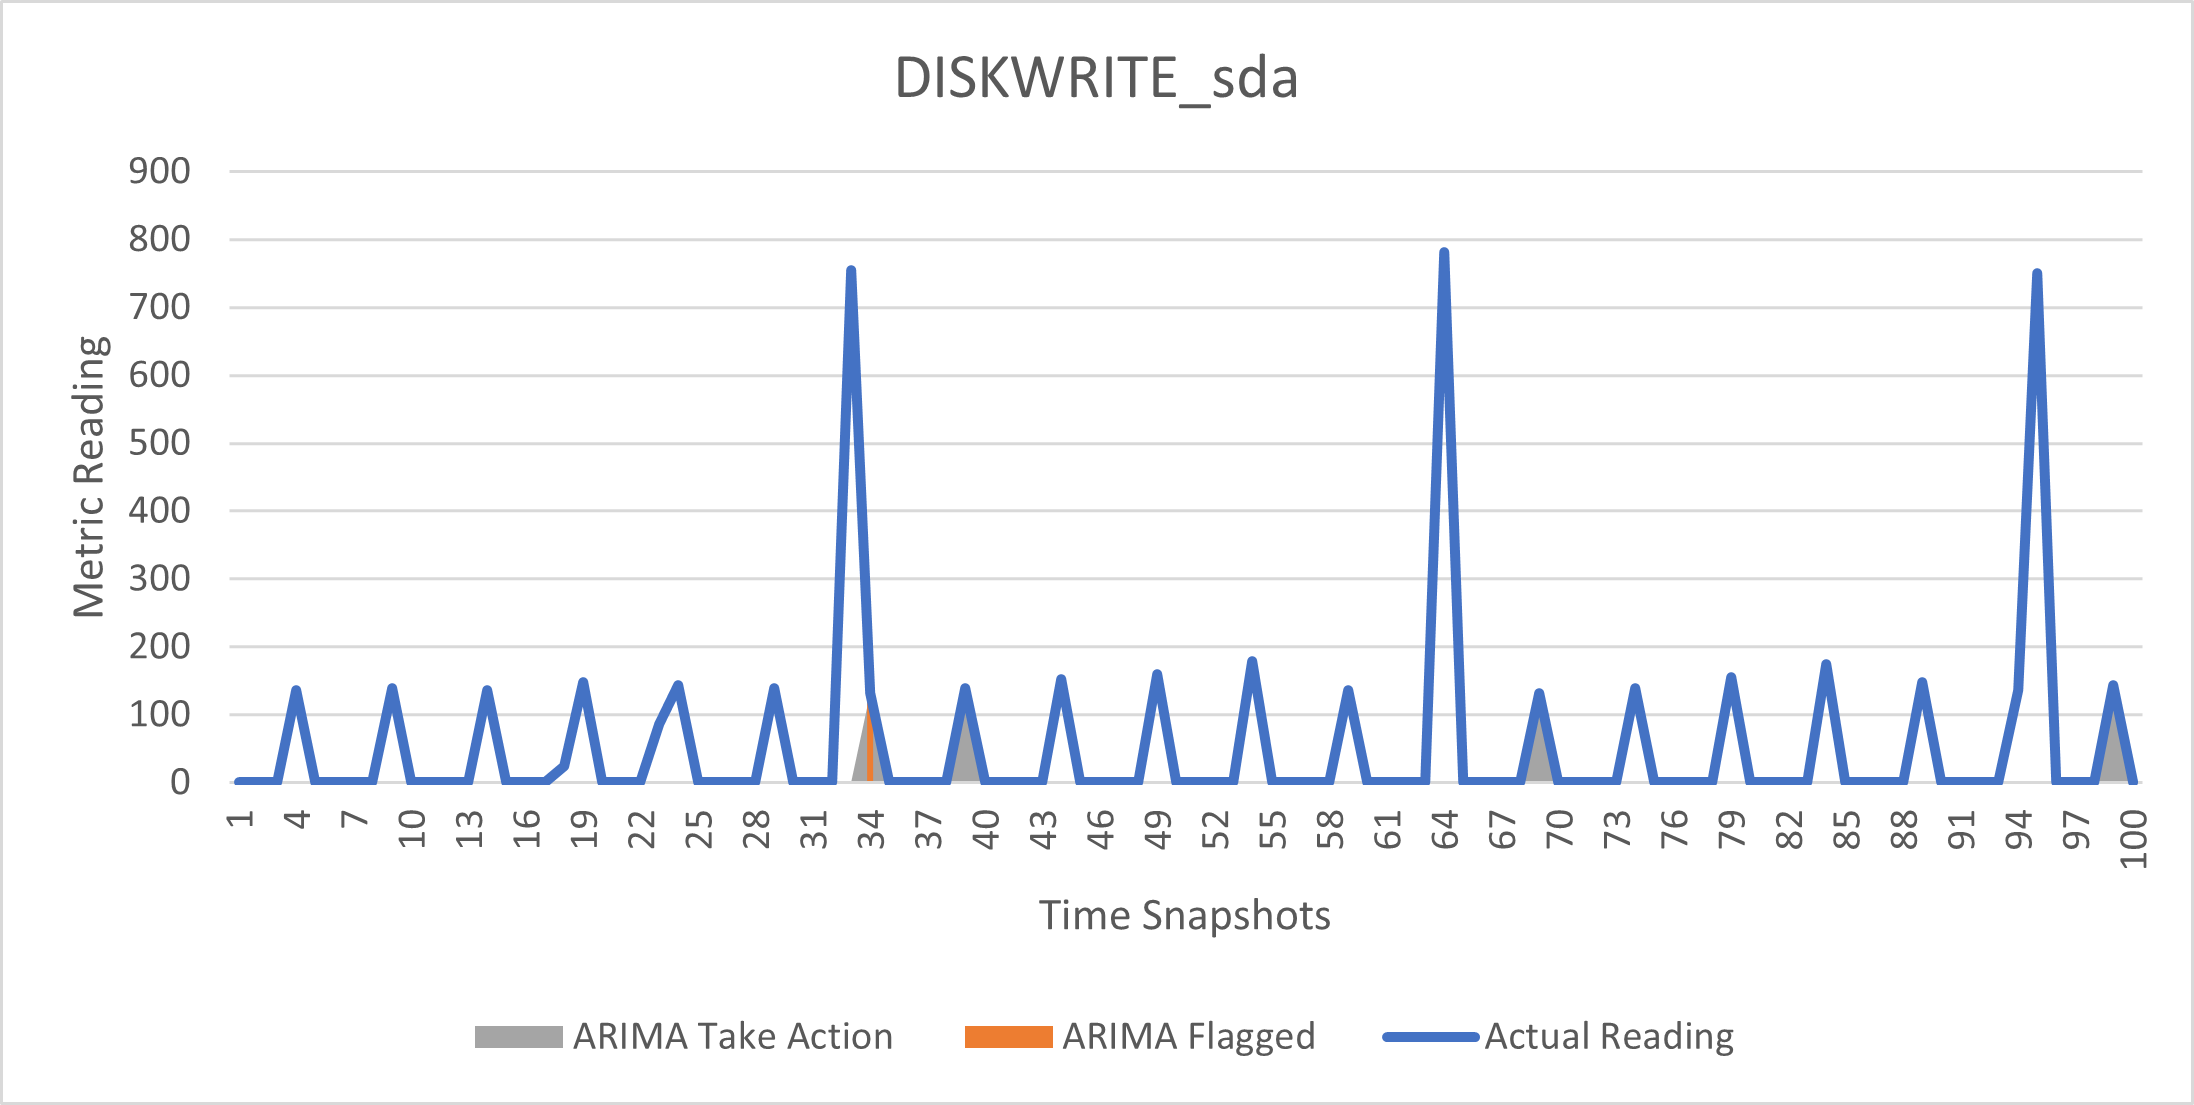
\includegraphics[width=\textwidth]{images/metrics_charts/30_pct_file_load/c1_s1/28.png}
         \caption{DISKWRITE\_sda | Adaptive Decision}
         \label{fig:c1_s1_28}
     \end{subfigure}
     \hfill
     \begin{subfigure}[ht]{0.49\textwidth}
         \centering
         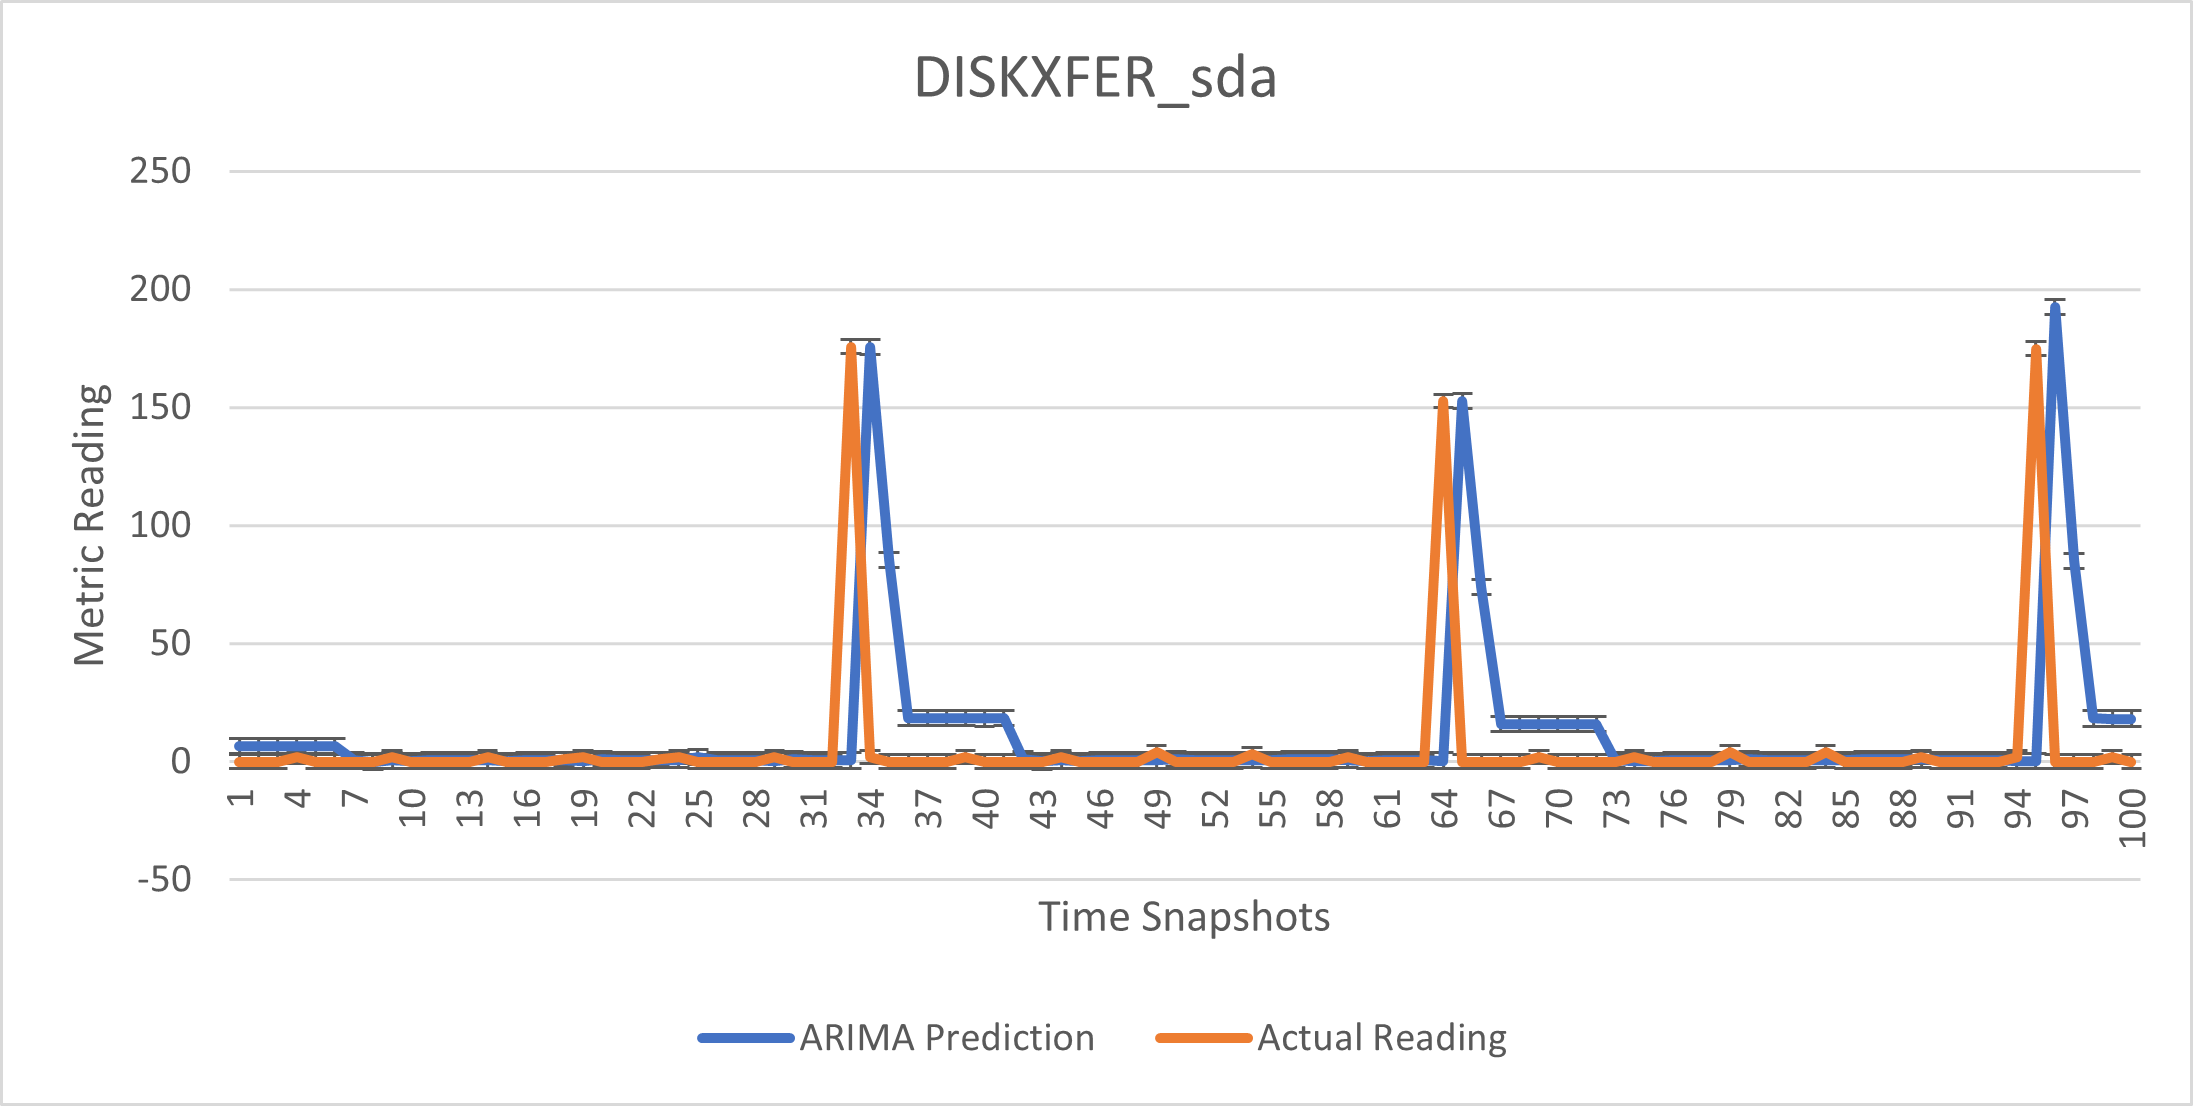
\includegraphics[width=\textwidth]{images/metrics_charts/30_pct_file_load/c1_s1/31.png}
         \caption{DISKXFER\_sda | ARIMA Prediction}
         \label{fig:c1_s1_31}
     \end{subfigure}
     \hfill
     \begin{subfigure}[ht]{0.49\textwidth}
         \centering
         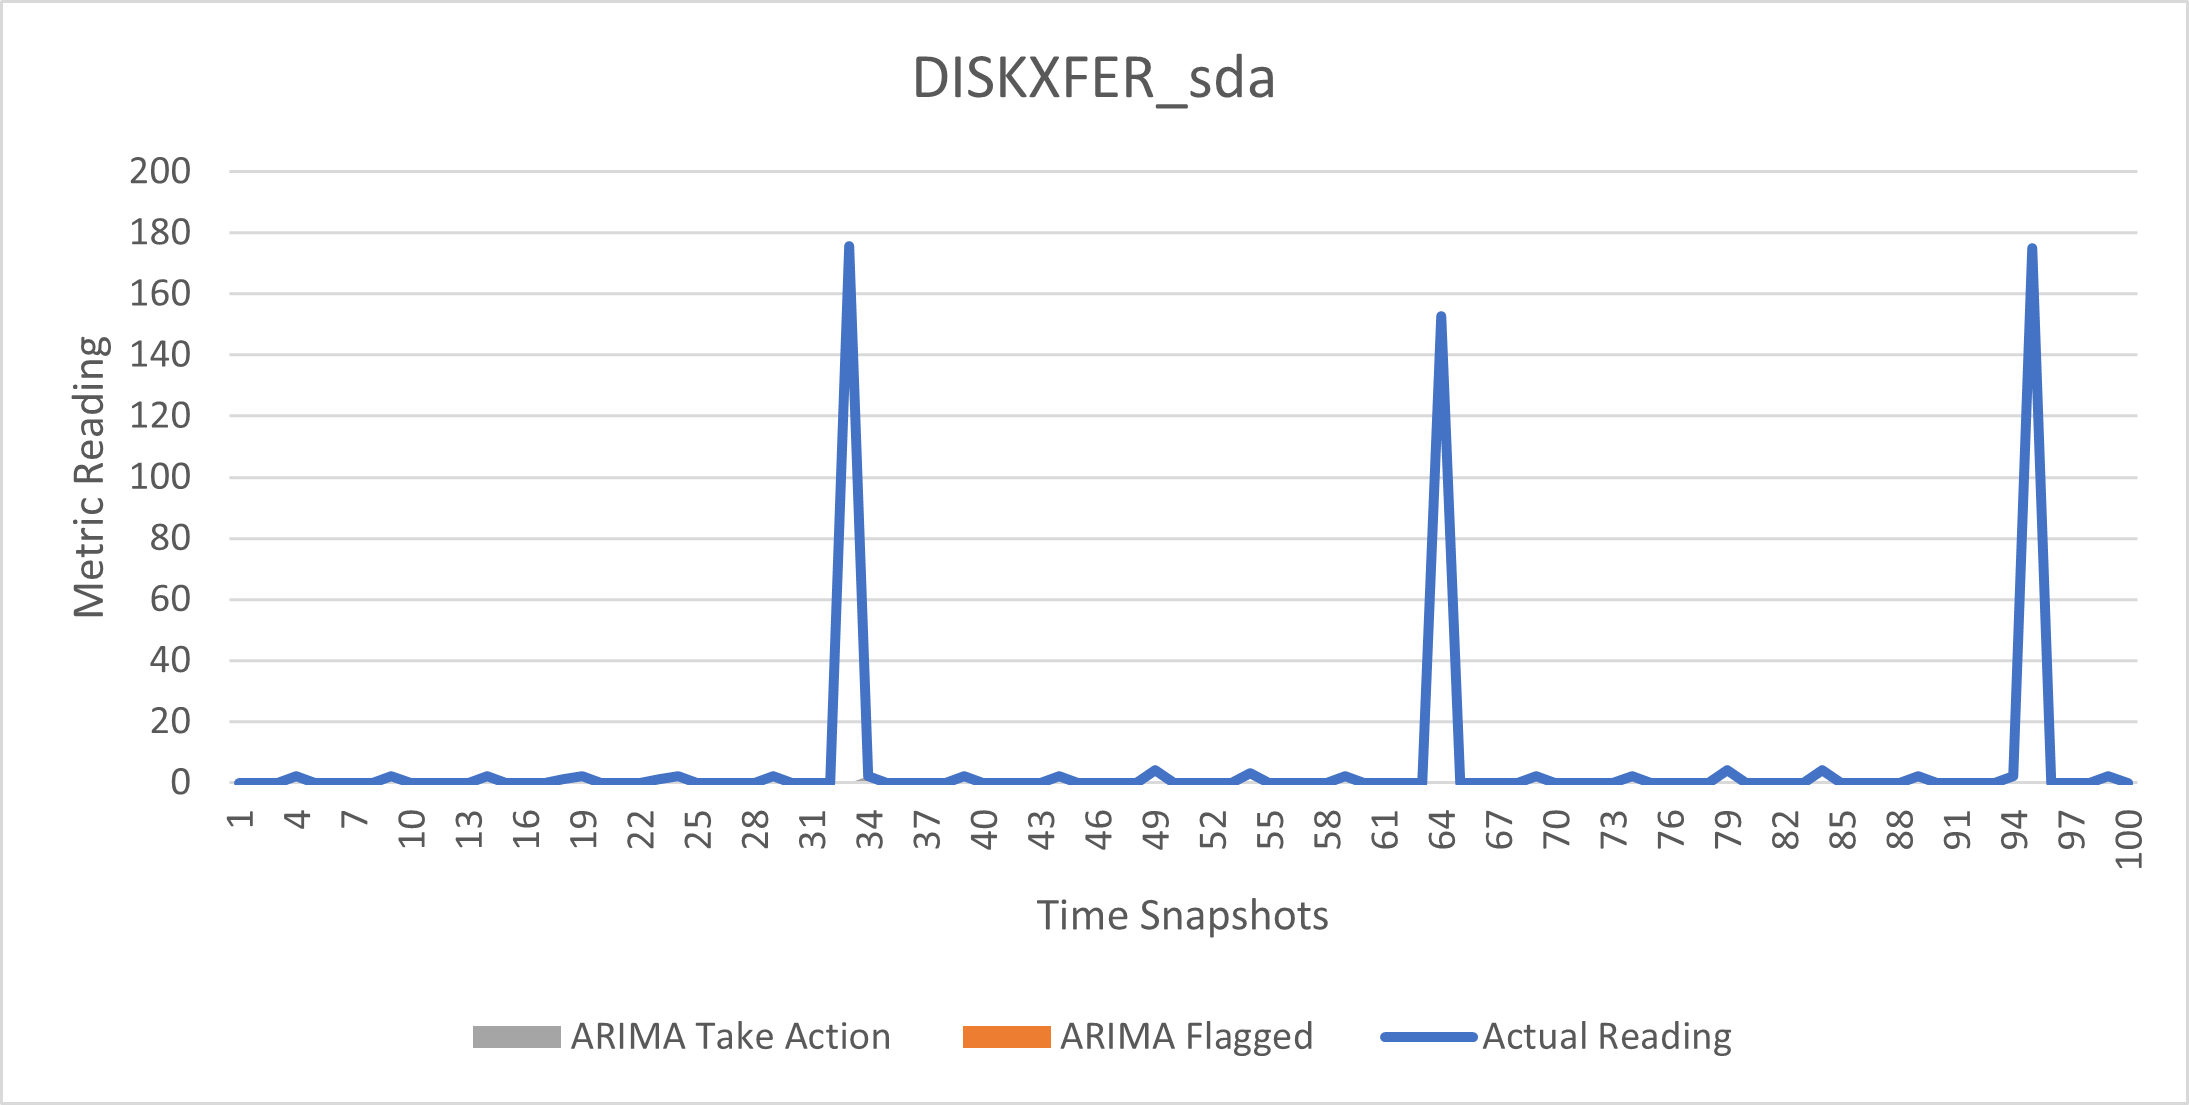
\includegraphics[width=\textwidth]{images/metrics_charts/30_pct_file_load/c1_s1/32.png}
         \caption{DISKXFER\_sda | Adaptive Decision}
         \label{fig:c1_s1_32}
     \end{subfigure}
     \hfill
     \caption{Disk Metrics For Partition Sda| Case Study: 1}
     \label{fig:c1_s1_disksda}
\end{figure*}

\begin{figure*}[tbp]
     \centering
     \begin{subfigure}[ht]{0.32\textwidth}
         \centering
         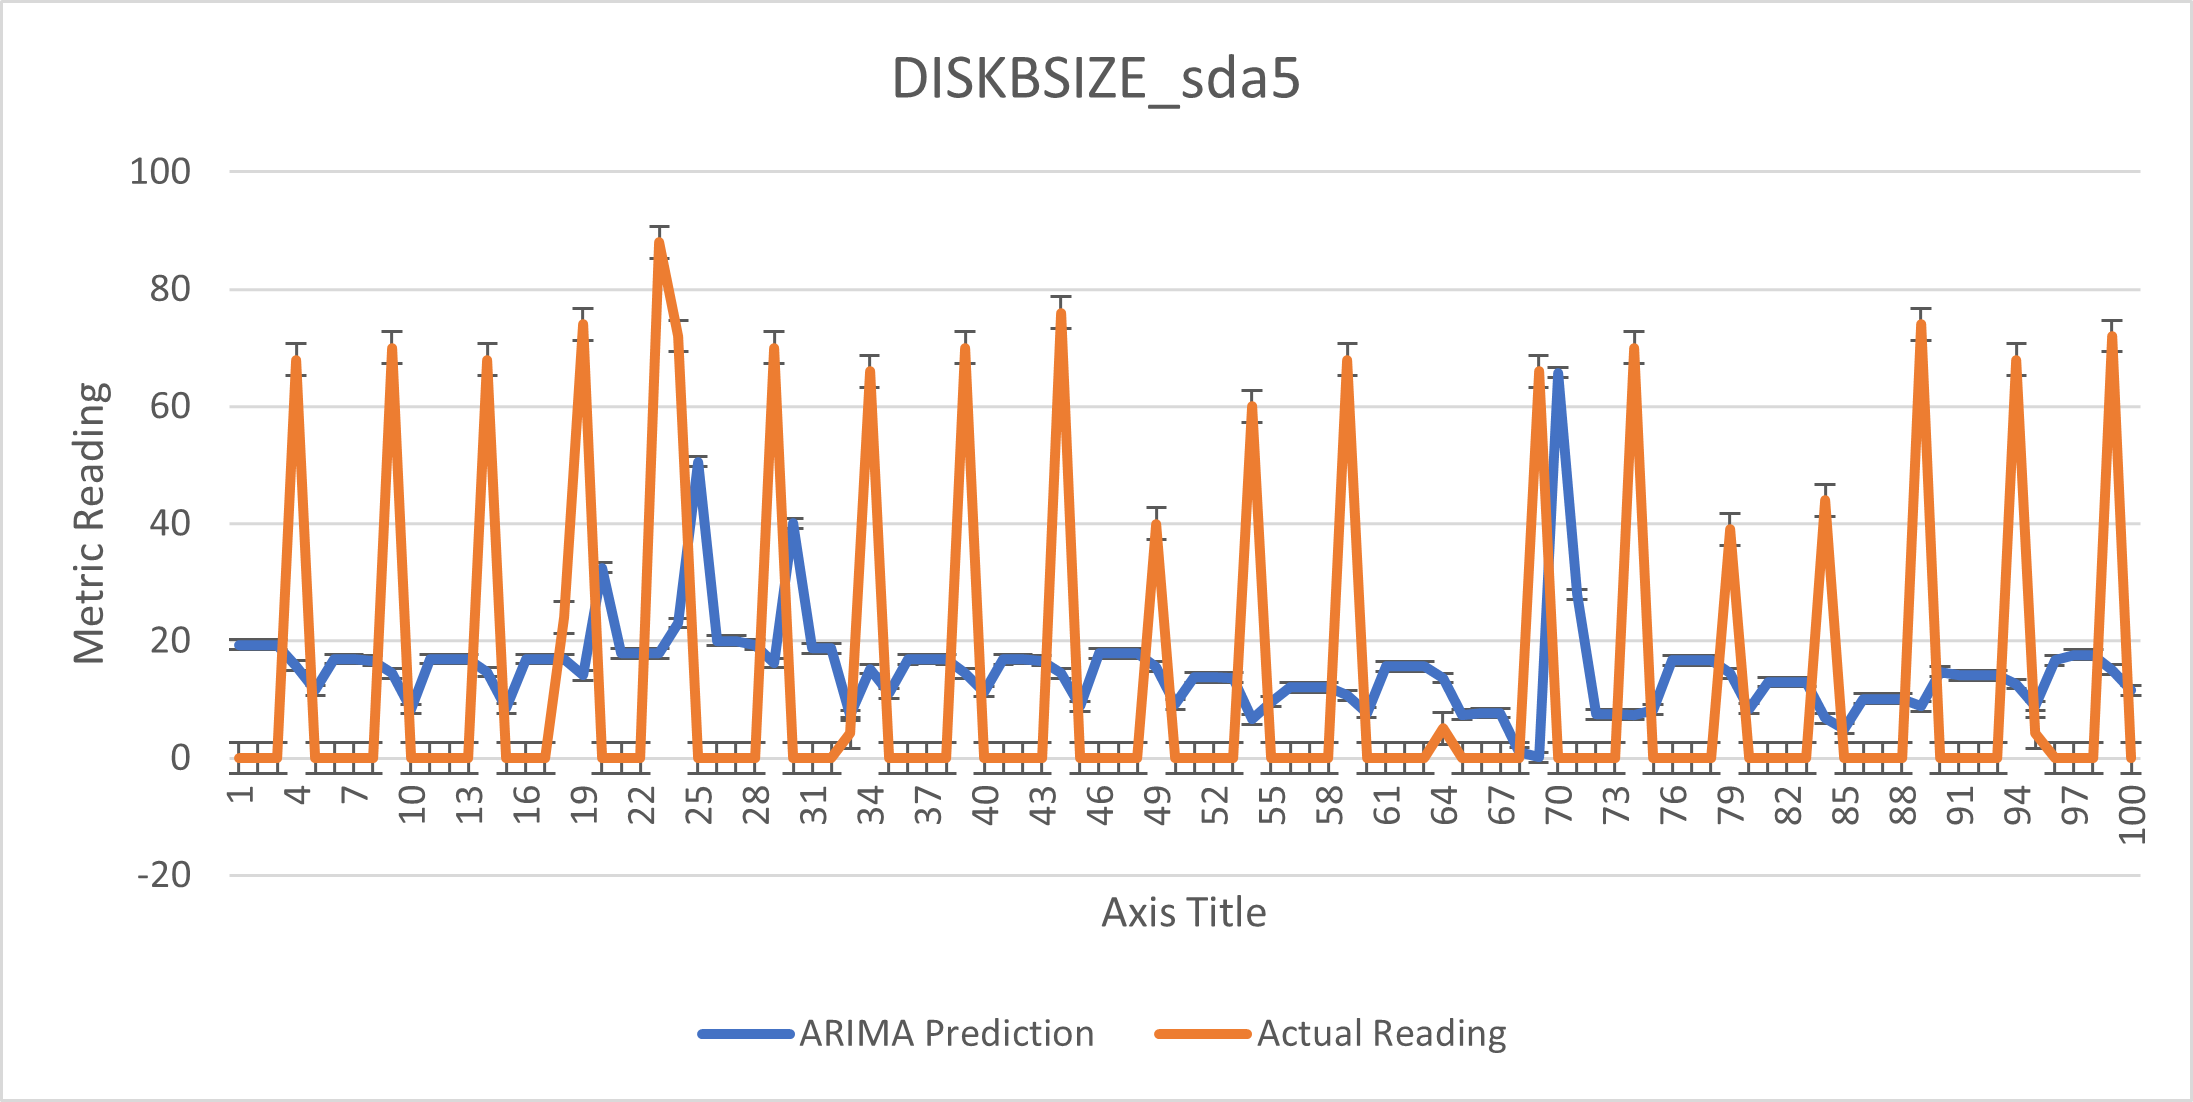
\includegraphics[width=\textwidth]{images/metrics_charts/30_pct_file_load/c1_s1/21.png}
         \caption{DISKBSIZE\_sda5 | ARIMA Prediction}
         \label{fig:c1_s1_21}
     \end{subfigure}
     \hfill
     \begin{subfigure}[ht]{0.32\textwidth}
         \centering
         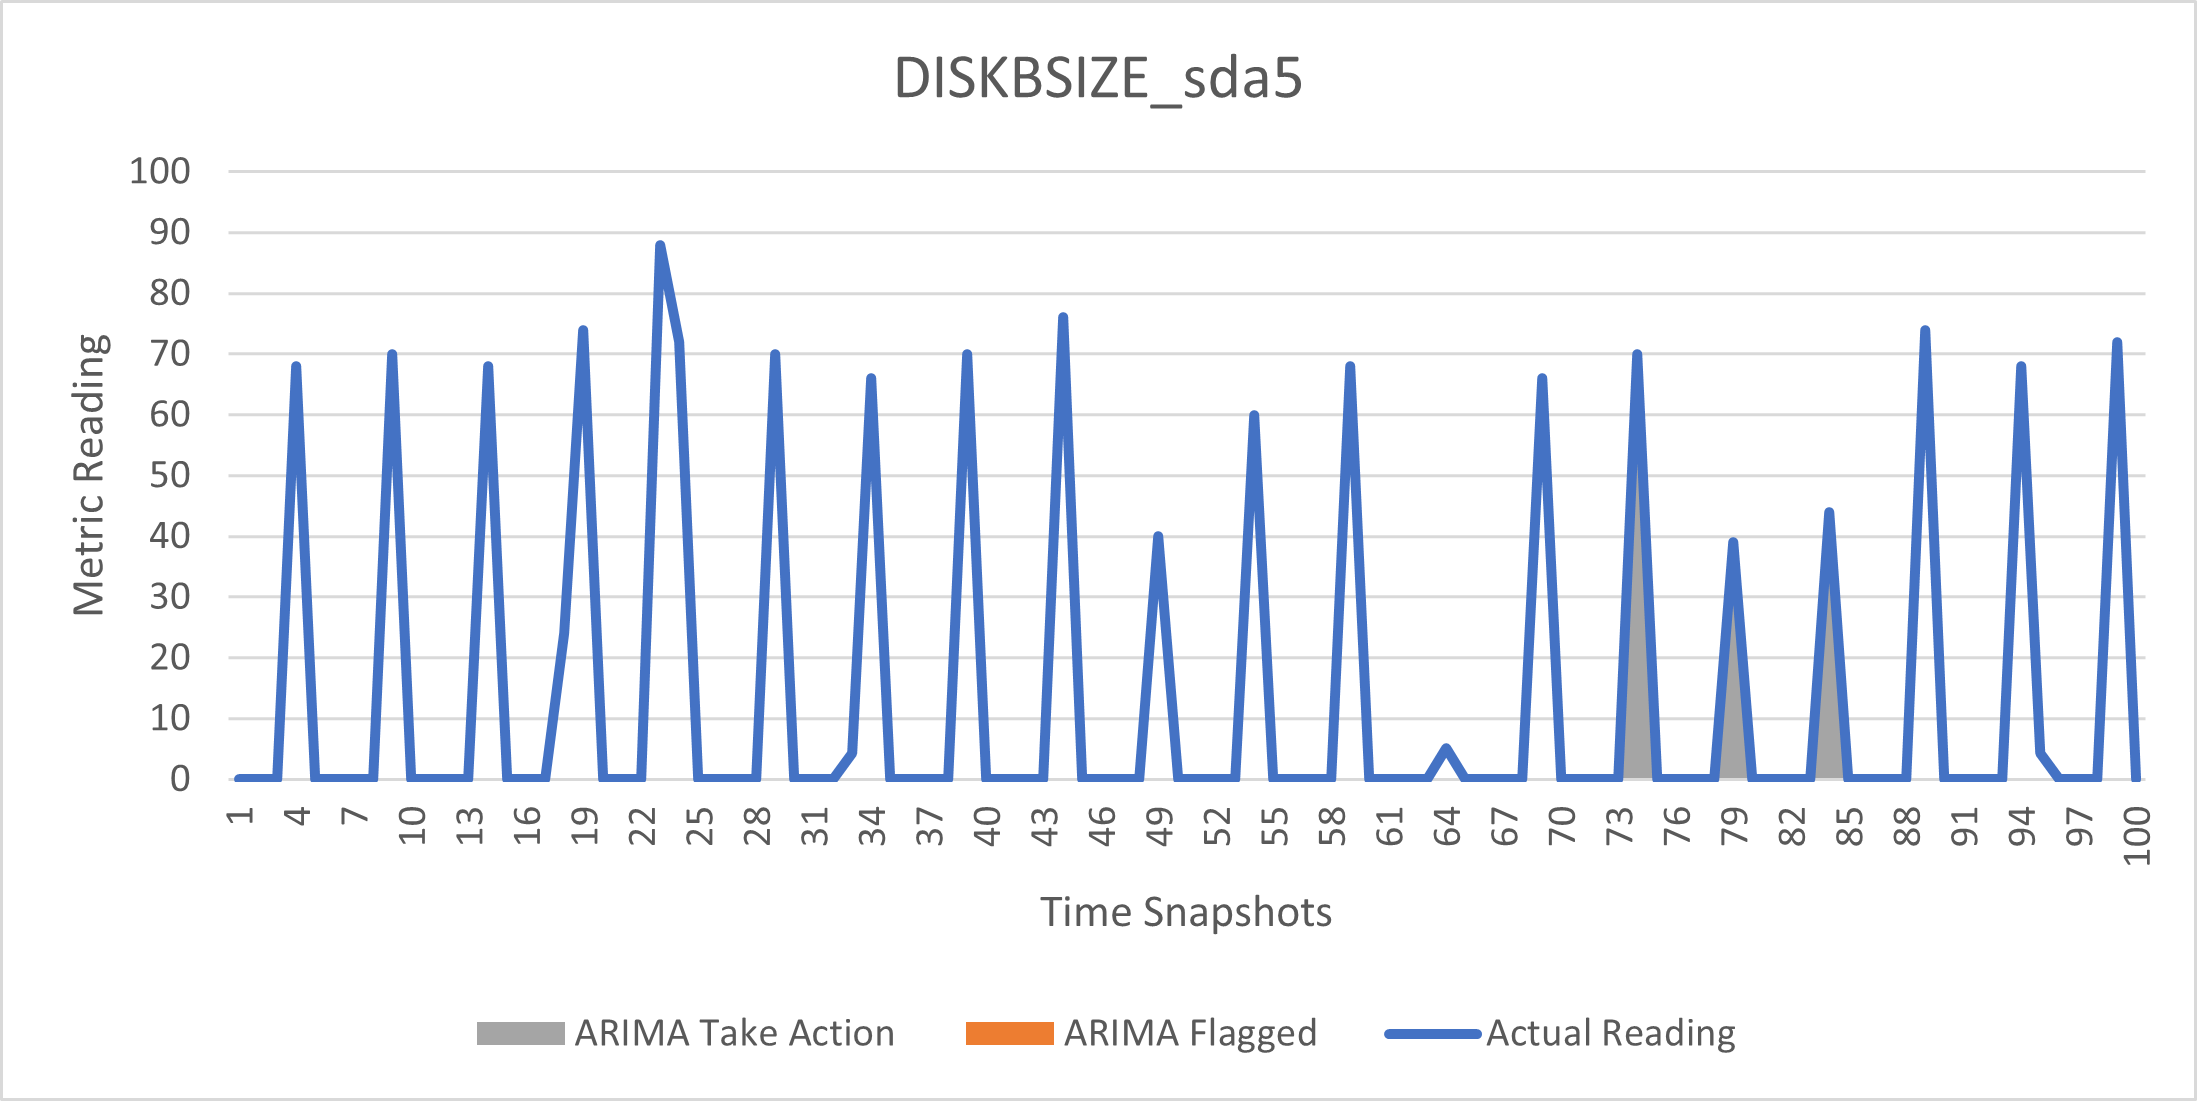
\includegraphics[width=\textwidth]{images/metrics_charts/30_pct_file_load/c1_s1/22.png}
         \caption{DISKBSIZE\_sda5 | Adaptive Decision}
         \label{fig:c1_s1_22}
     \end{subfigure}
     \hfill
     \begin{subfigure}[ht]{0.32\textwidth}
         \centering
         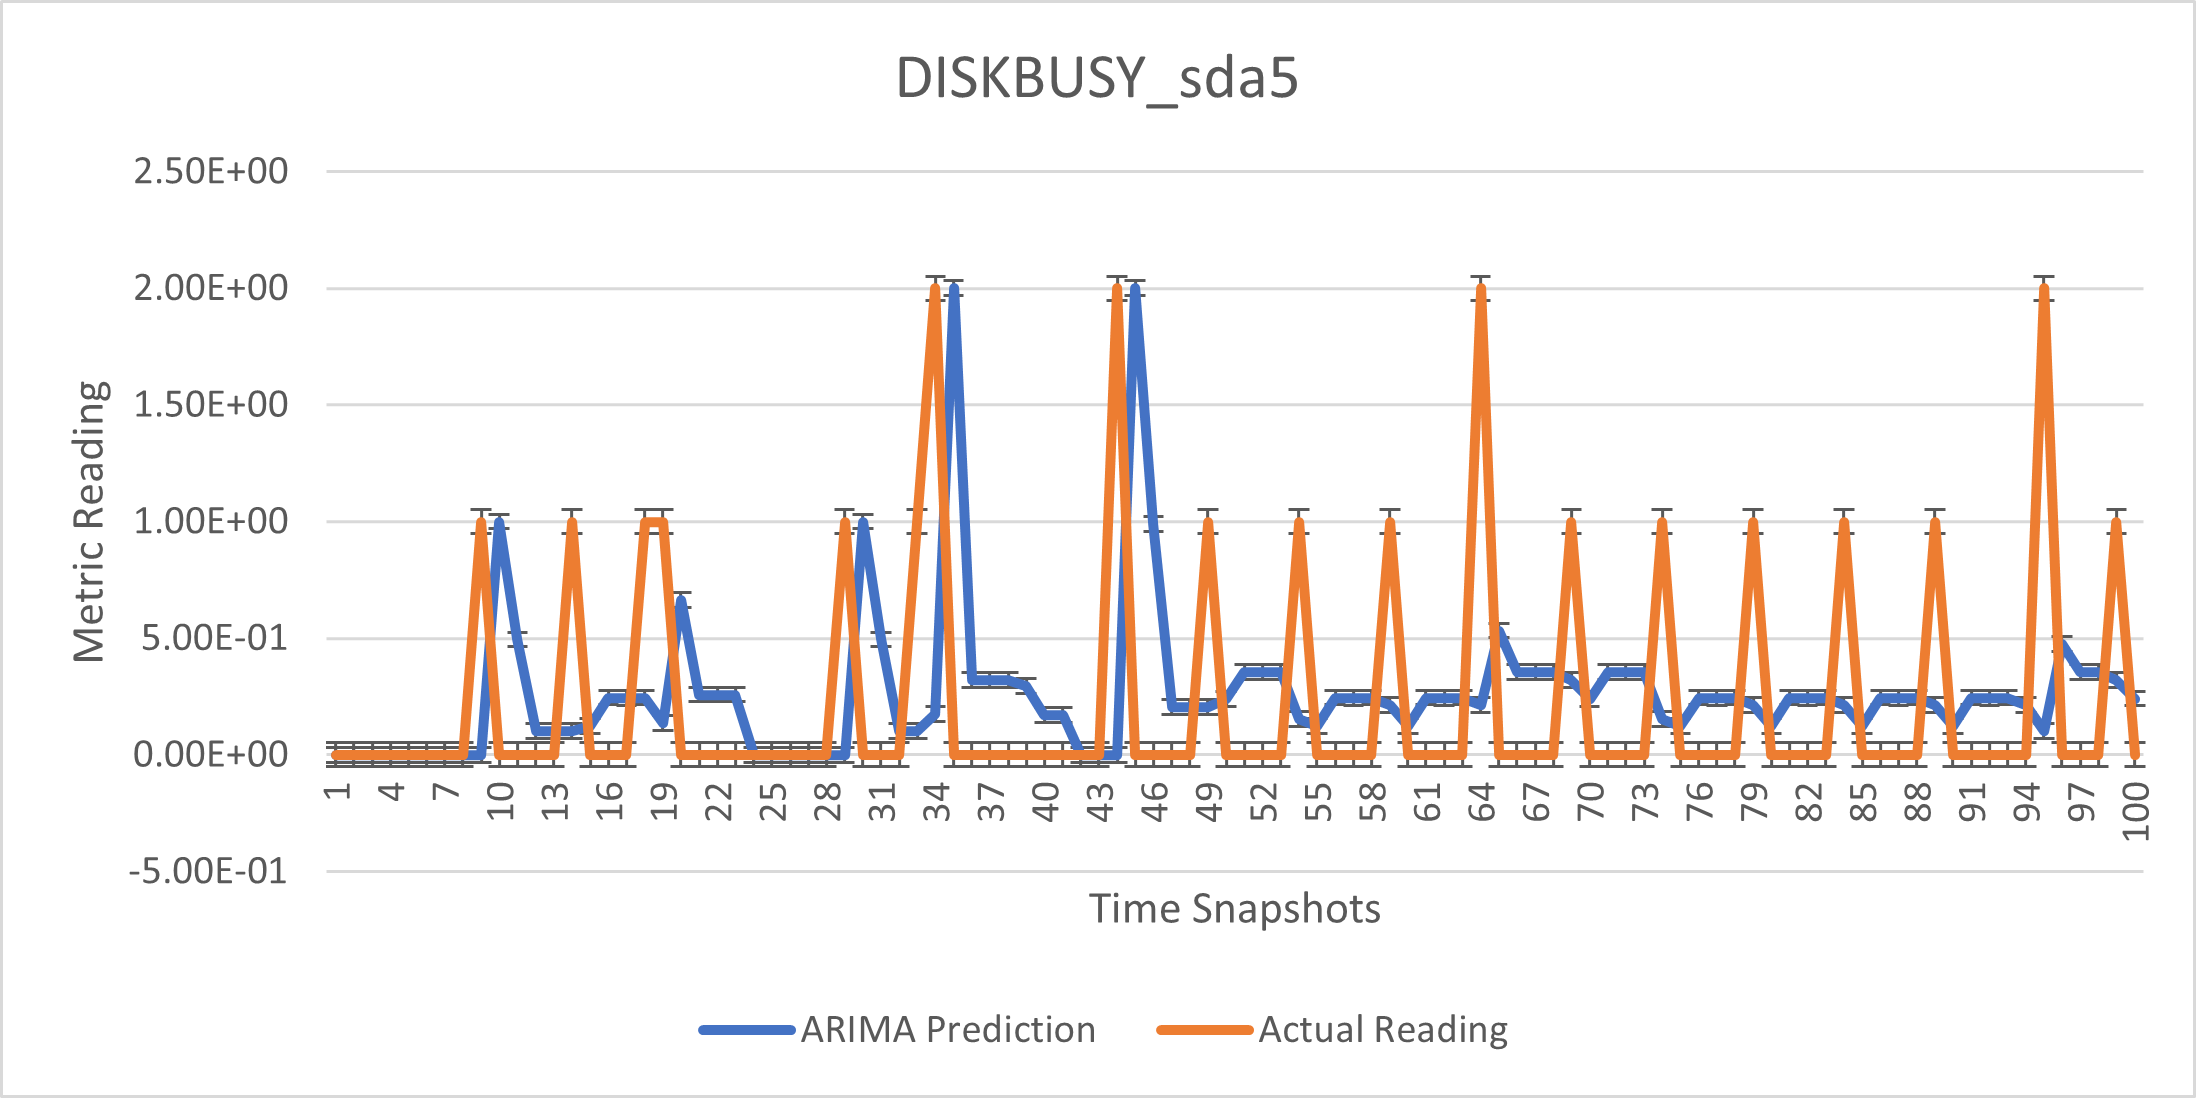
\includegraphics[width=\textwidth]{images/metrics_charts/30_pct_file_load/c1_s1/25.png}
         \caption{DISKBUSY\_sda5 | ARIMA Prediction}
         \label{fig:c1_s1_25}
     \end{subfigure}
     \hfill
     \begin{subfigure}[ht]{0.32\textwidth}
         \centering
         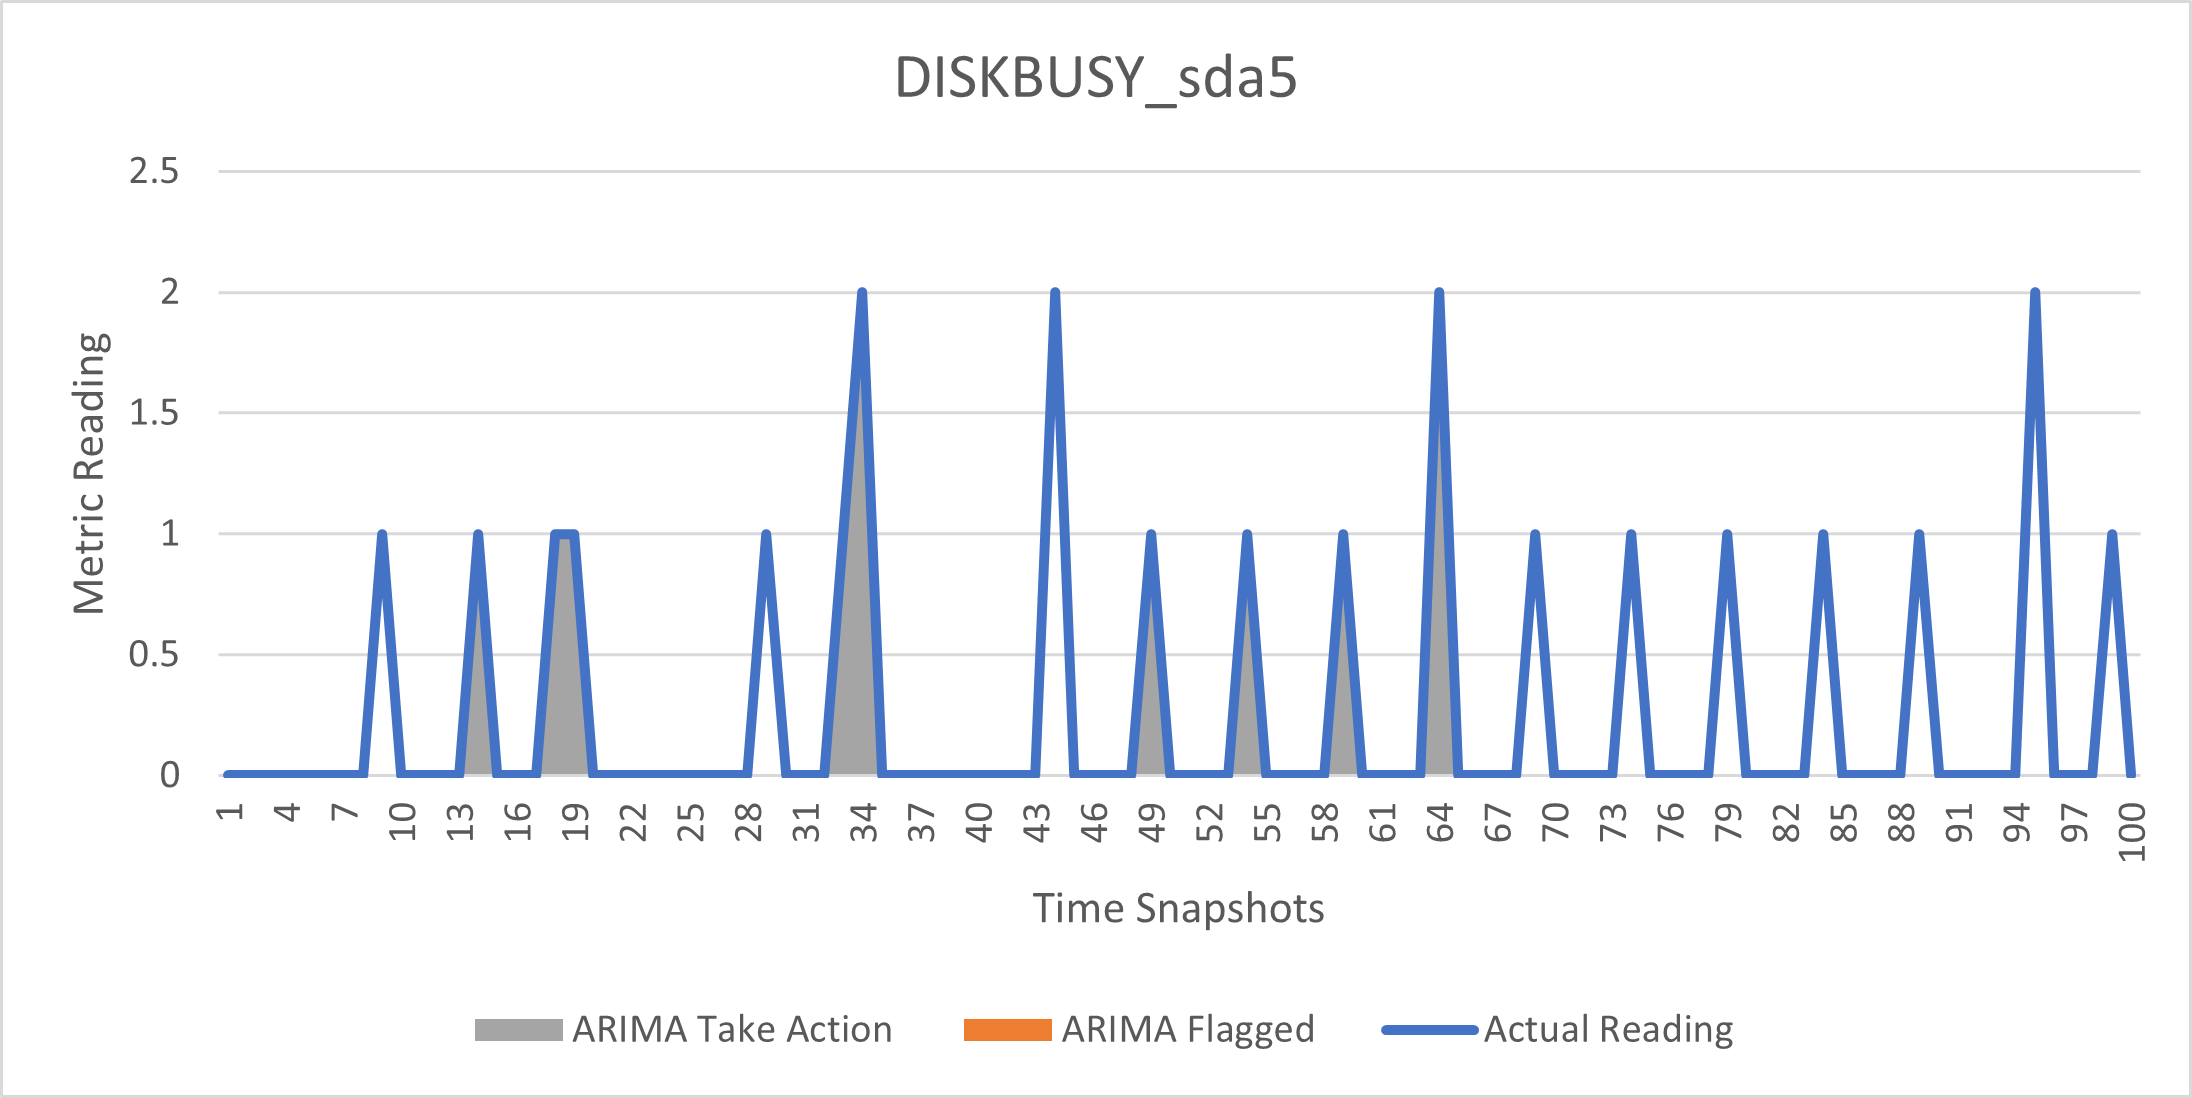
\includegraphics[width=\textwidth]{images/metrics_charts/30_pct_file_load/c1_s1/26.png}
         \caption{DISKBUSY\_sda5 | Adaptive Decision}
         \label{fig:c1_s1_26}
     \end{subfigure}
     \hfill
     \begin{subfigure}[ht]{0.32\textwidth}
         \centering
         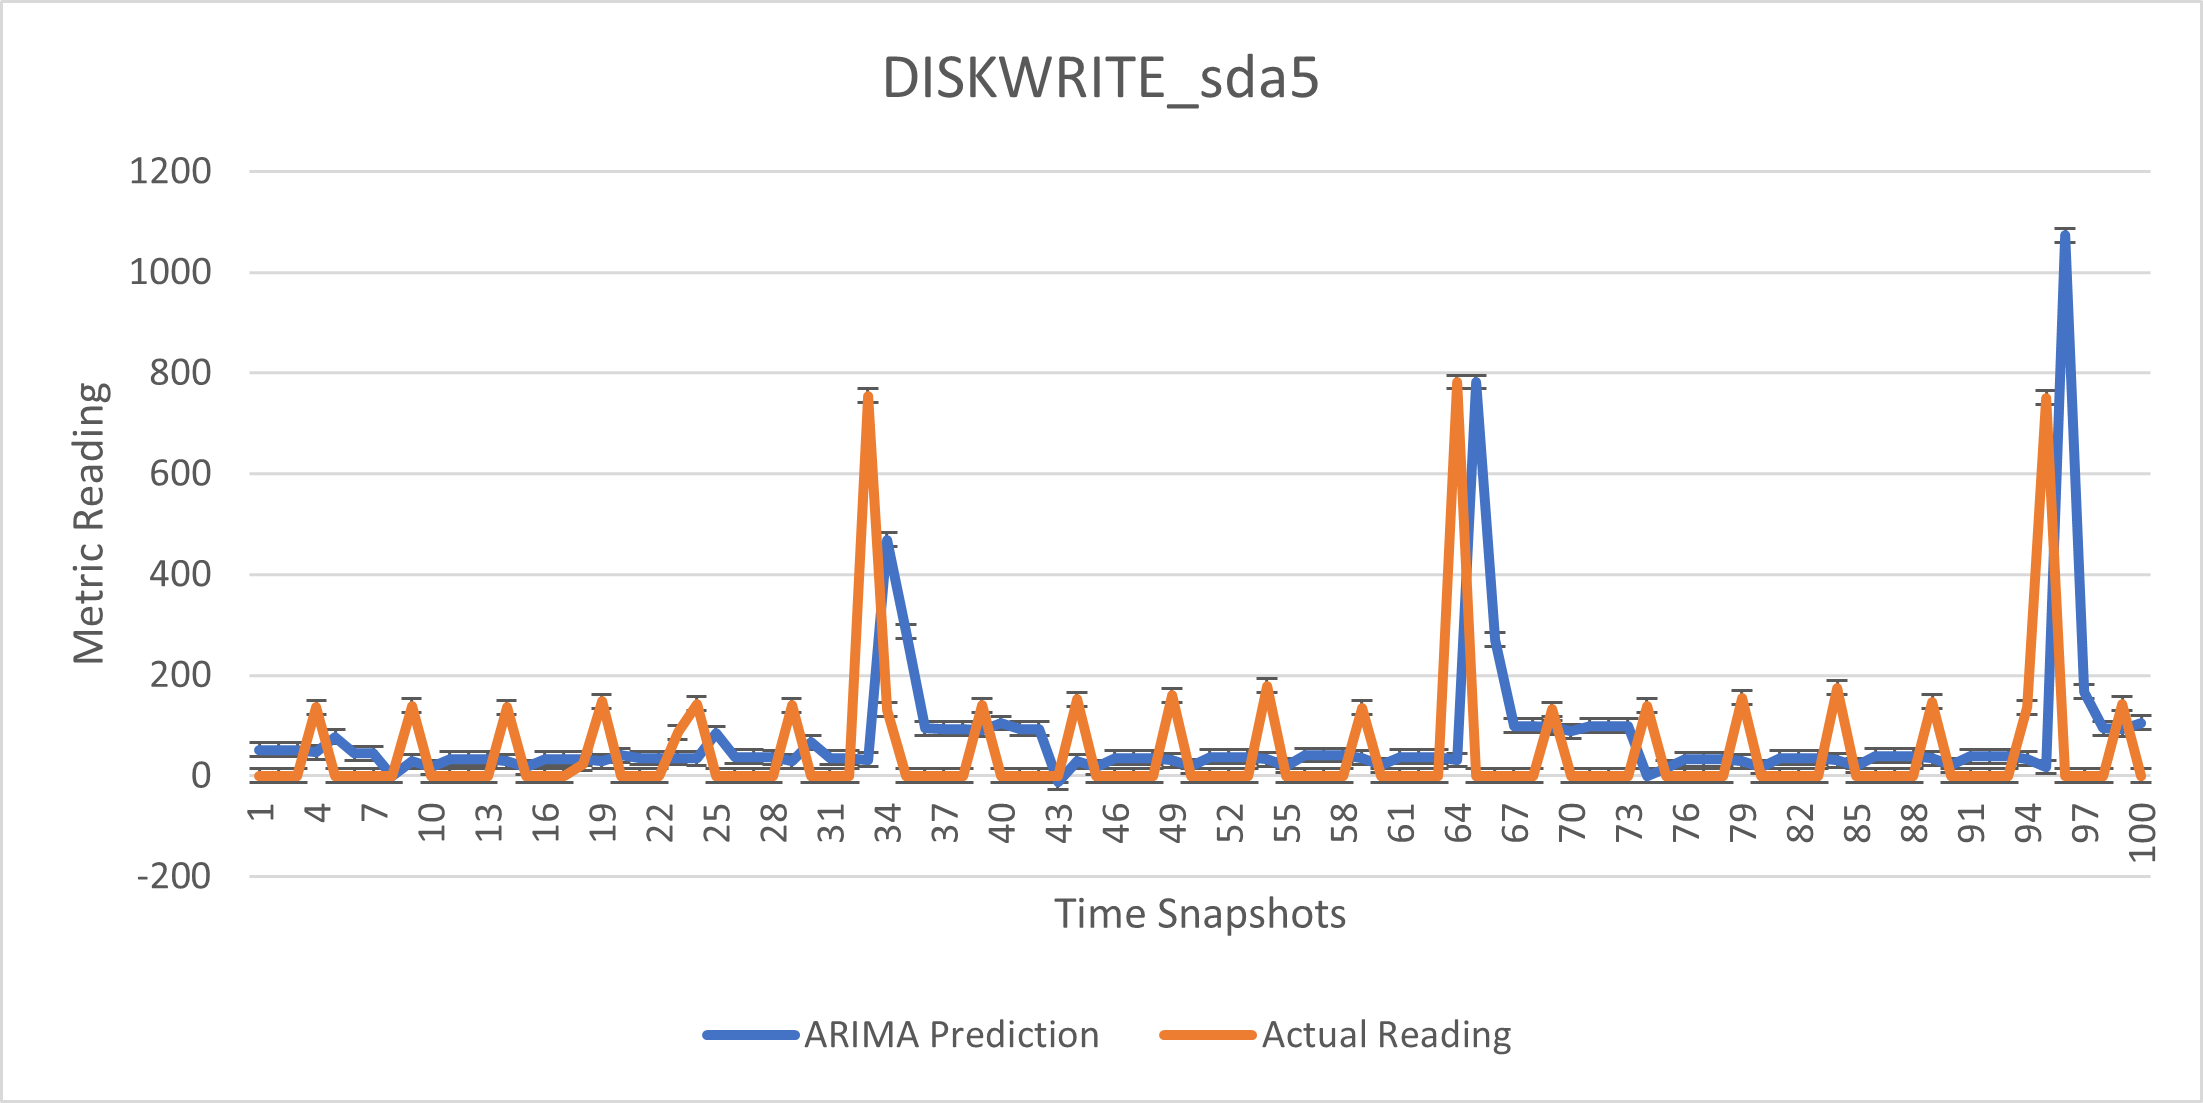
\includegraphics[width=\textwidth]{images/metrics_charts/30_pct_file_load/c1_s1/29.png}
         \caption{DISKWRITE\_sda5 | ARIMA Prediction}
         \label{fig:c1_s1_29}
     \end{subfigure}
     \hfill
     \begin{subfigure}[ht]{0.32\textwidth}
         \centering
         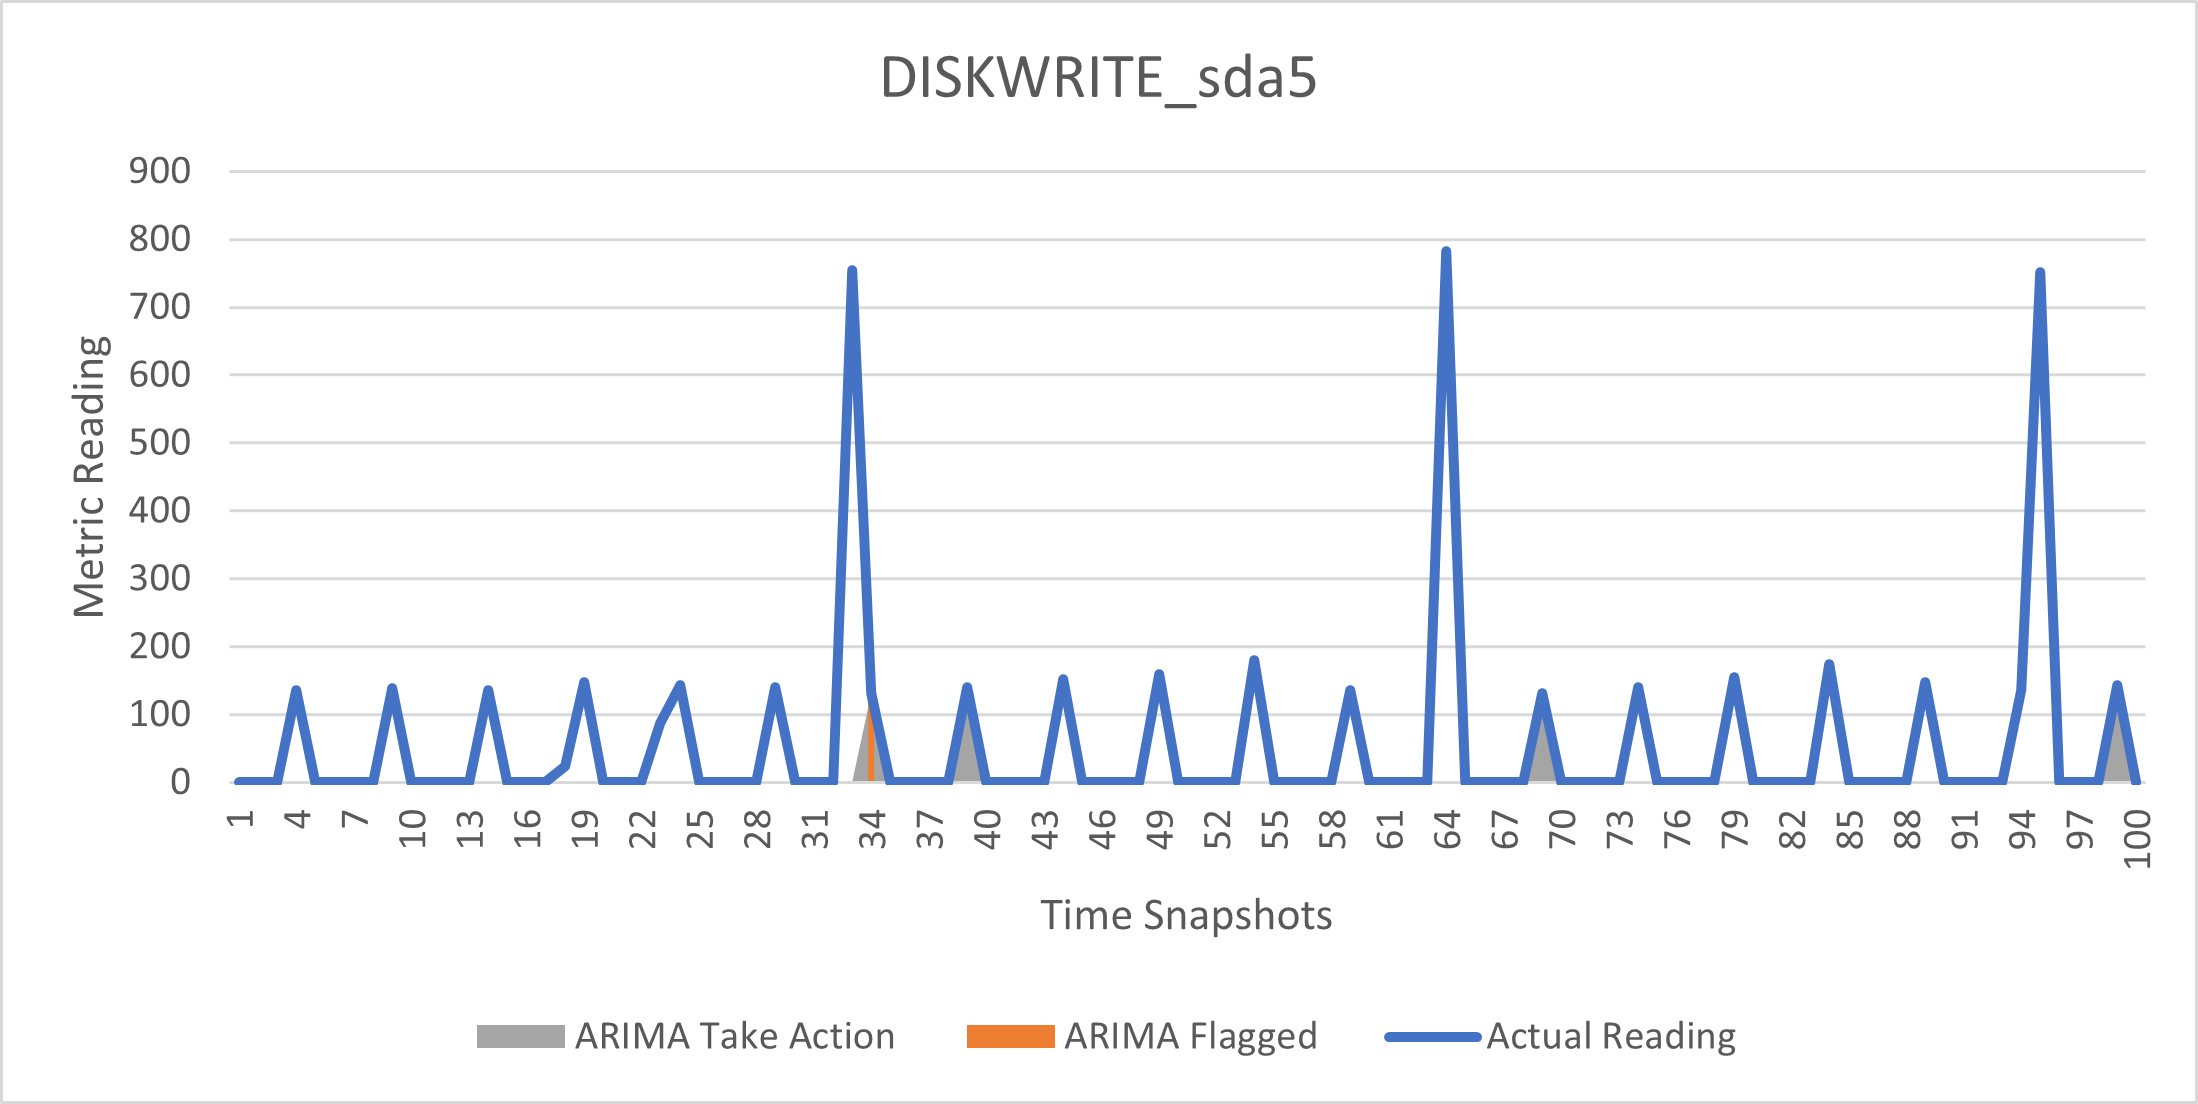
\includegraphics[width=\textwidth]{images/metrics_charts/30_pct_file_load/c1_s1/30.png}
         \caption{DISKWRITE\_sda5 | Adaptive Decision}
         \label{fig:c1_s1_30}
     \end{subfigure}
     \hfill
     \begin{subfigure}[ht]{0.49\textwidth}
         \centering
         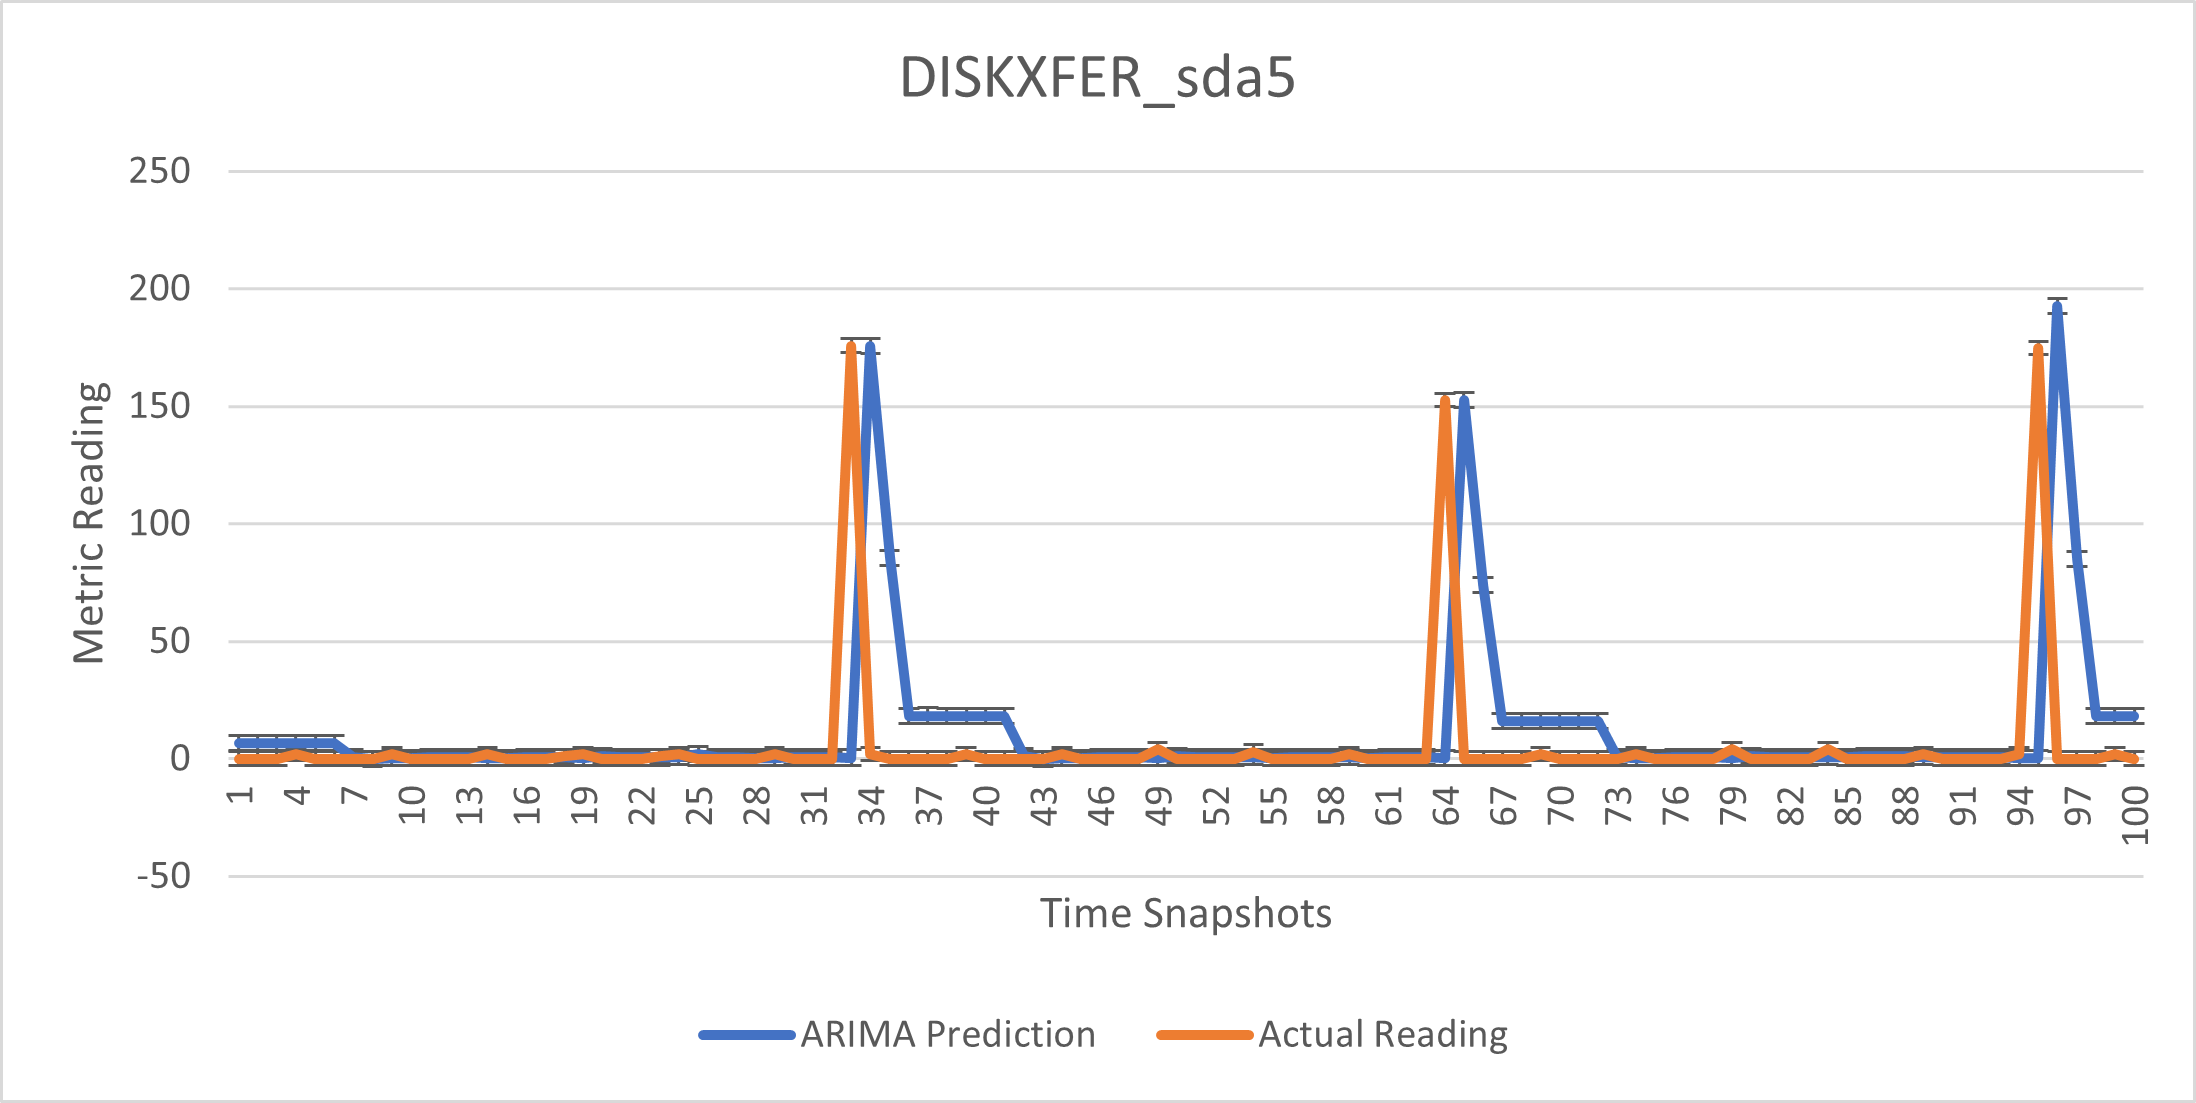
\includegraphics[width=\textwidth]{images/metrics_charts/30_pct_file_load/c1_s1/33.png}
         \caption{DISKXFER\_sda5 | ARIMA Prediction}
         \label{fig:c1_s1_33}
     \end{subfigure}
     \hfill
     \begin{subfigure}[ht]{0.49\textwidth}
         \centering
         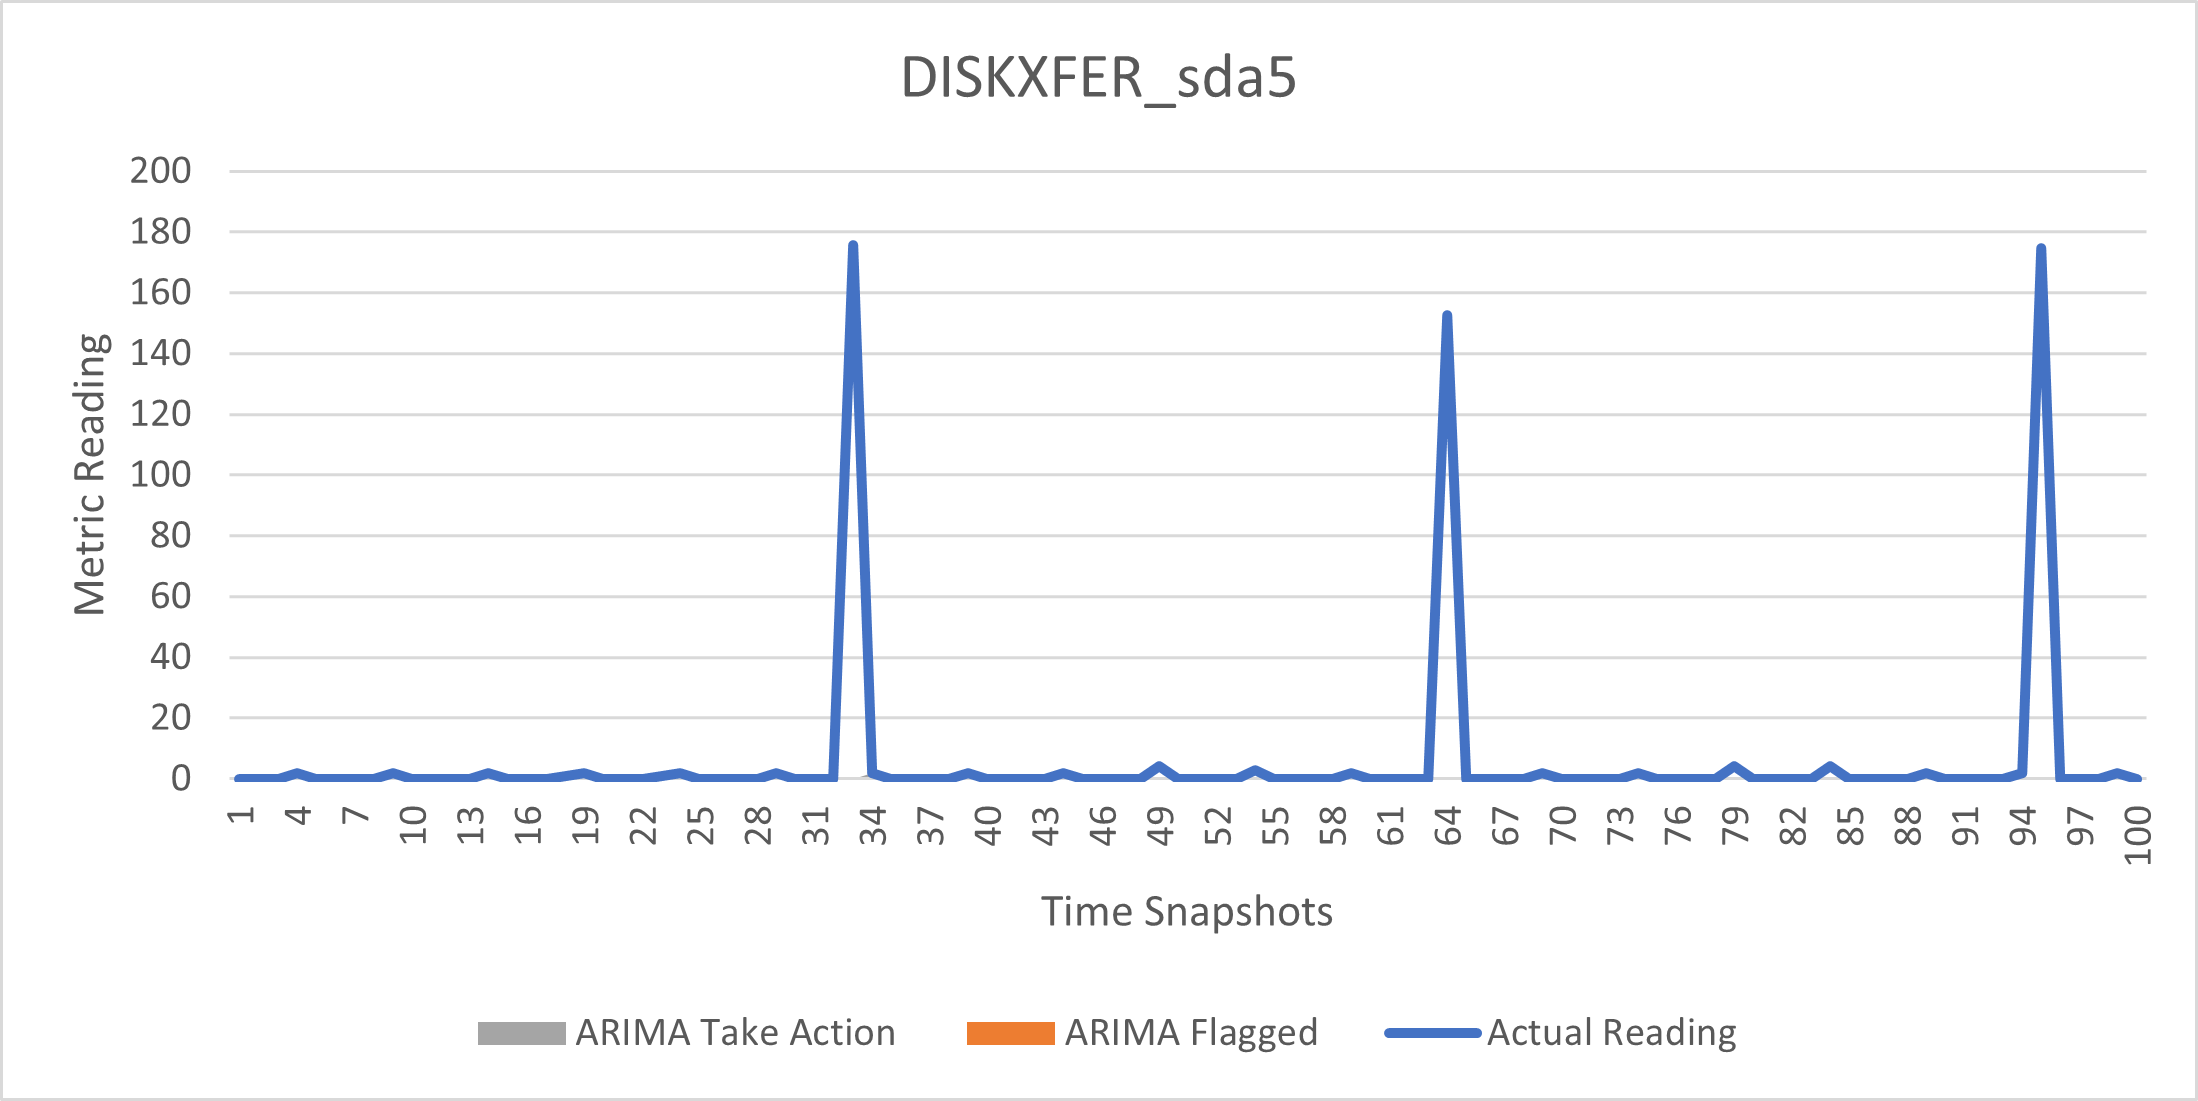
\includegraphics[width=\textwidth]{images/metrics_charts/30_pct_file_load/c1_s1/34.png}
         \caption{DISKXFER\_sda5 | Adaptive Decision}
         \label{fig:c1_s1_34}
     \end{subfigure}
     \hfill
     \caption{Disk Metrics For Partition Sda5 | Case Study: 1}
     \label{fig:c1_s1_disksda5}
\end{figure*}

Figure \ref{fig:c1_s1_network} shows the network-related metrics of the system. We had only one active and enabled network interface named enp0s3. The network-related metrics could be categorized into NET and NETPACKET. The differences between them are that NET metrics show the overall usage in terms of read and write in KB/s, while NETPACKET metrics show the overall usage in terms of read and write but in the number of packets per second. From Figure \ref{fig:c1_s1_36} and \ref{fig:c1_s1_38}, we can see that both read and write for NET metrics were flagged at around the same timing; however, with a small amount of lag on NET writes. This is justifiable because the requests were sent first, followed by the echoing back of the large text from the text file and the prime numbers. Therefore, the write is supposed to see its pressure buildup later than the read. Like NET, the NETPACKET's read and write also sees the same pattern as when it first suggested taking action by our proposed approach for adaptive tracing. However, in general, we can see that for both NET and NETPACKET, the write had more time snapshot areas marked for taking action, which is in line with the experiment as whenever that 30\% probability was hit to echo out the large text file, the write metrics would see a sudden break of past trend in data being sent out through the network interface.

\begin{figure*}[tbp]
     \centering
     \begin{subfigure}[ht]{0.32\textwidth}
         \centering
         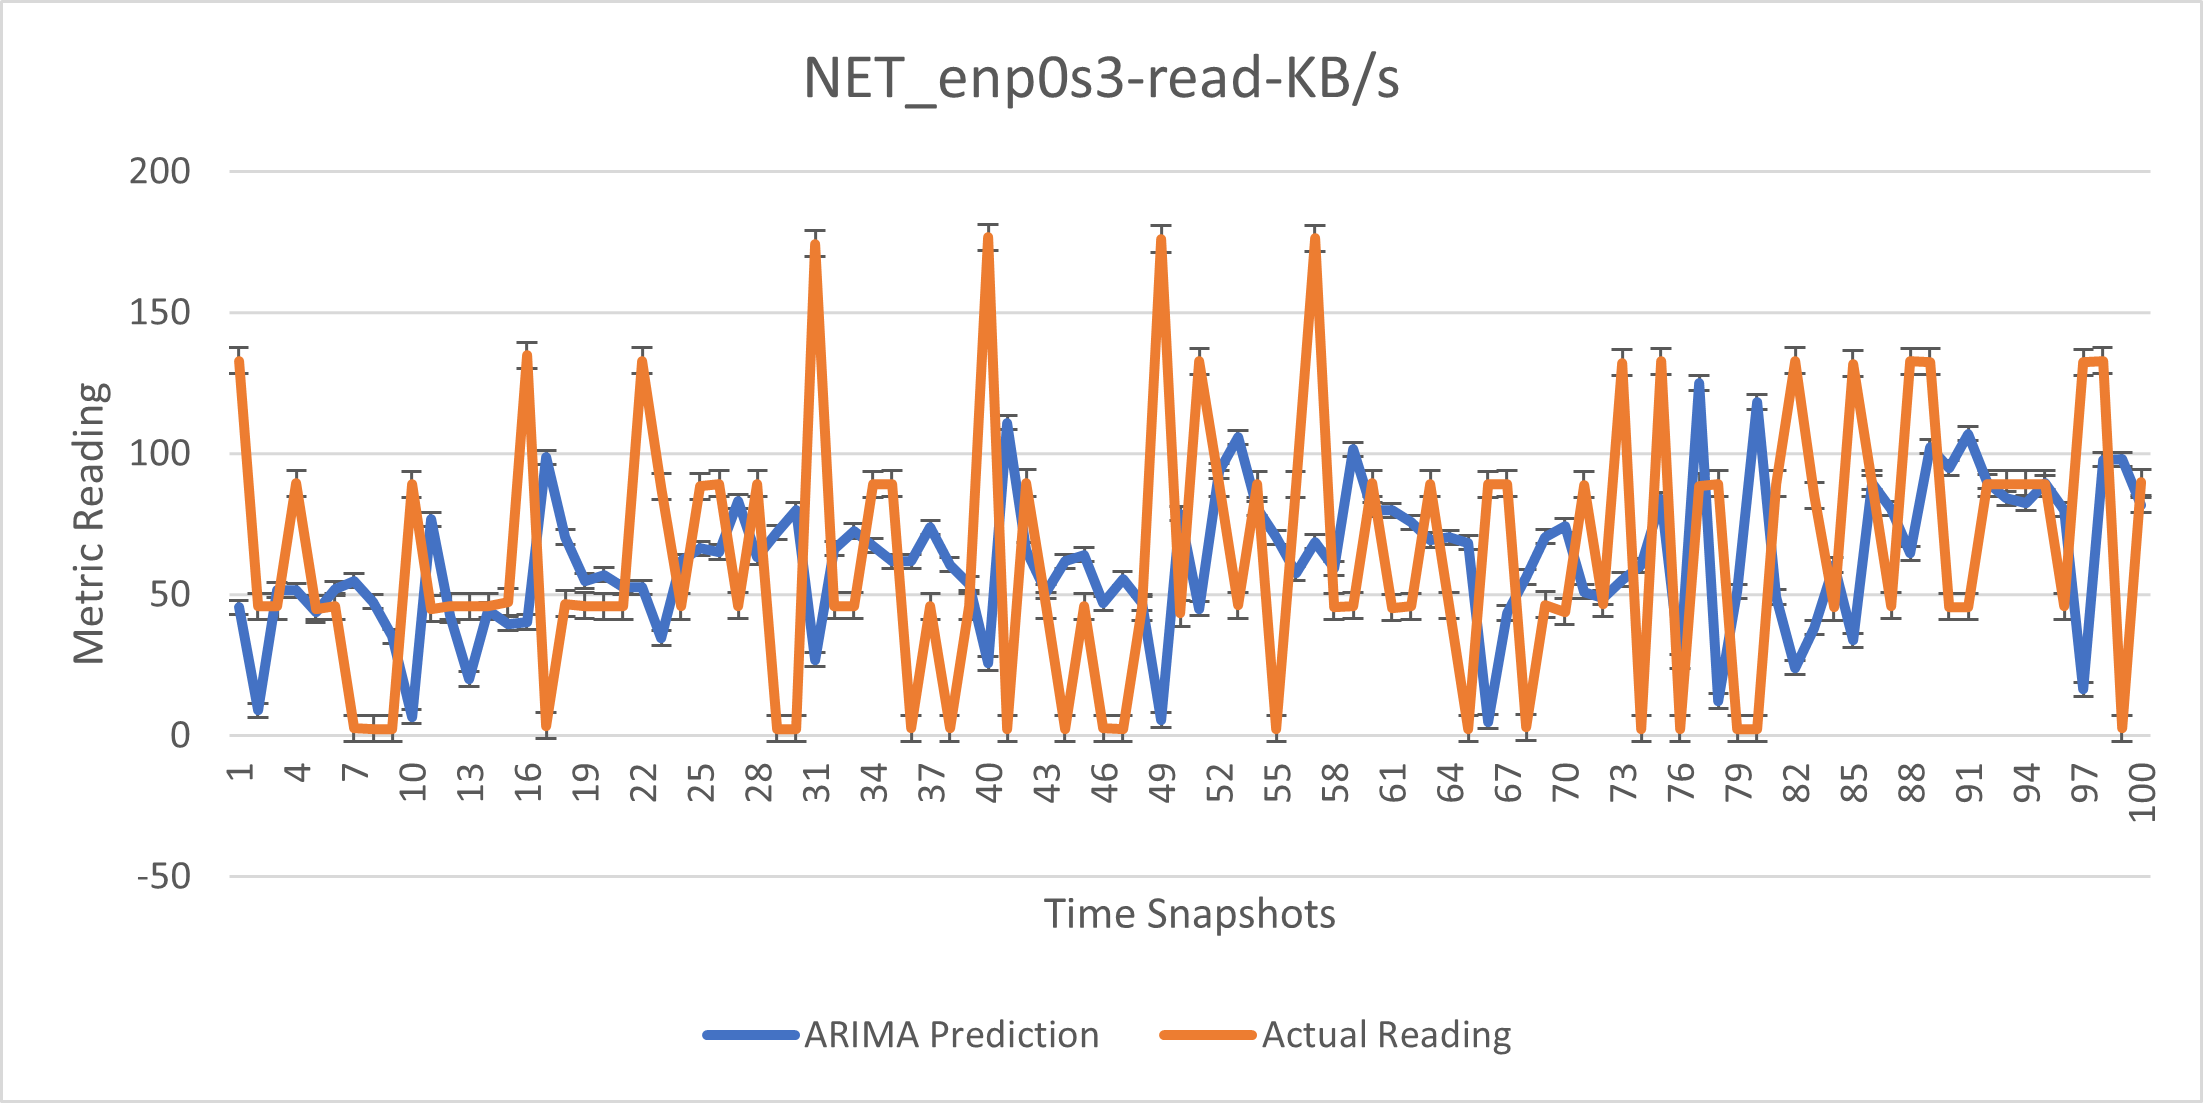
\includegraphics[width=\textwidth]{images/metrics_charts/30_pct_file_load/c1_s1/35.png}
         \caption{NET-read-KB/s | ARIMA Prediction}
         \label{fig:c1_s1_35}
     \end{subfigure}
     \hfill
     \begin{subfigure}[ht]{0.32\textwidth}
         \centering
         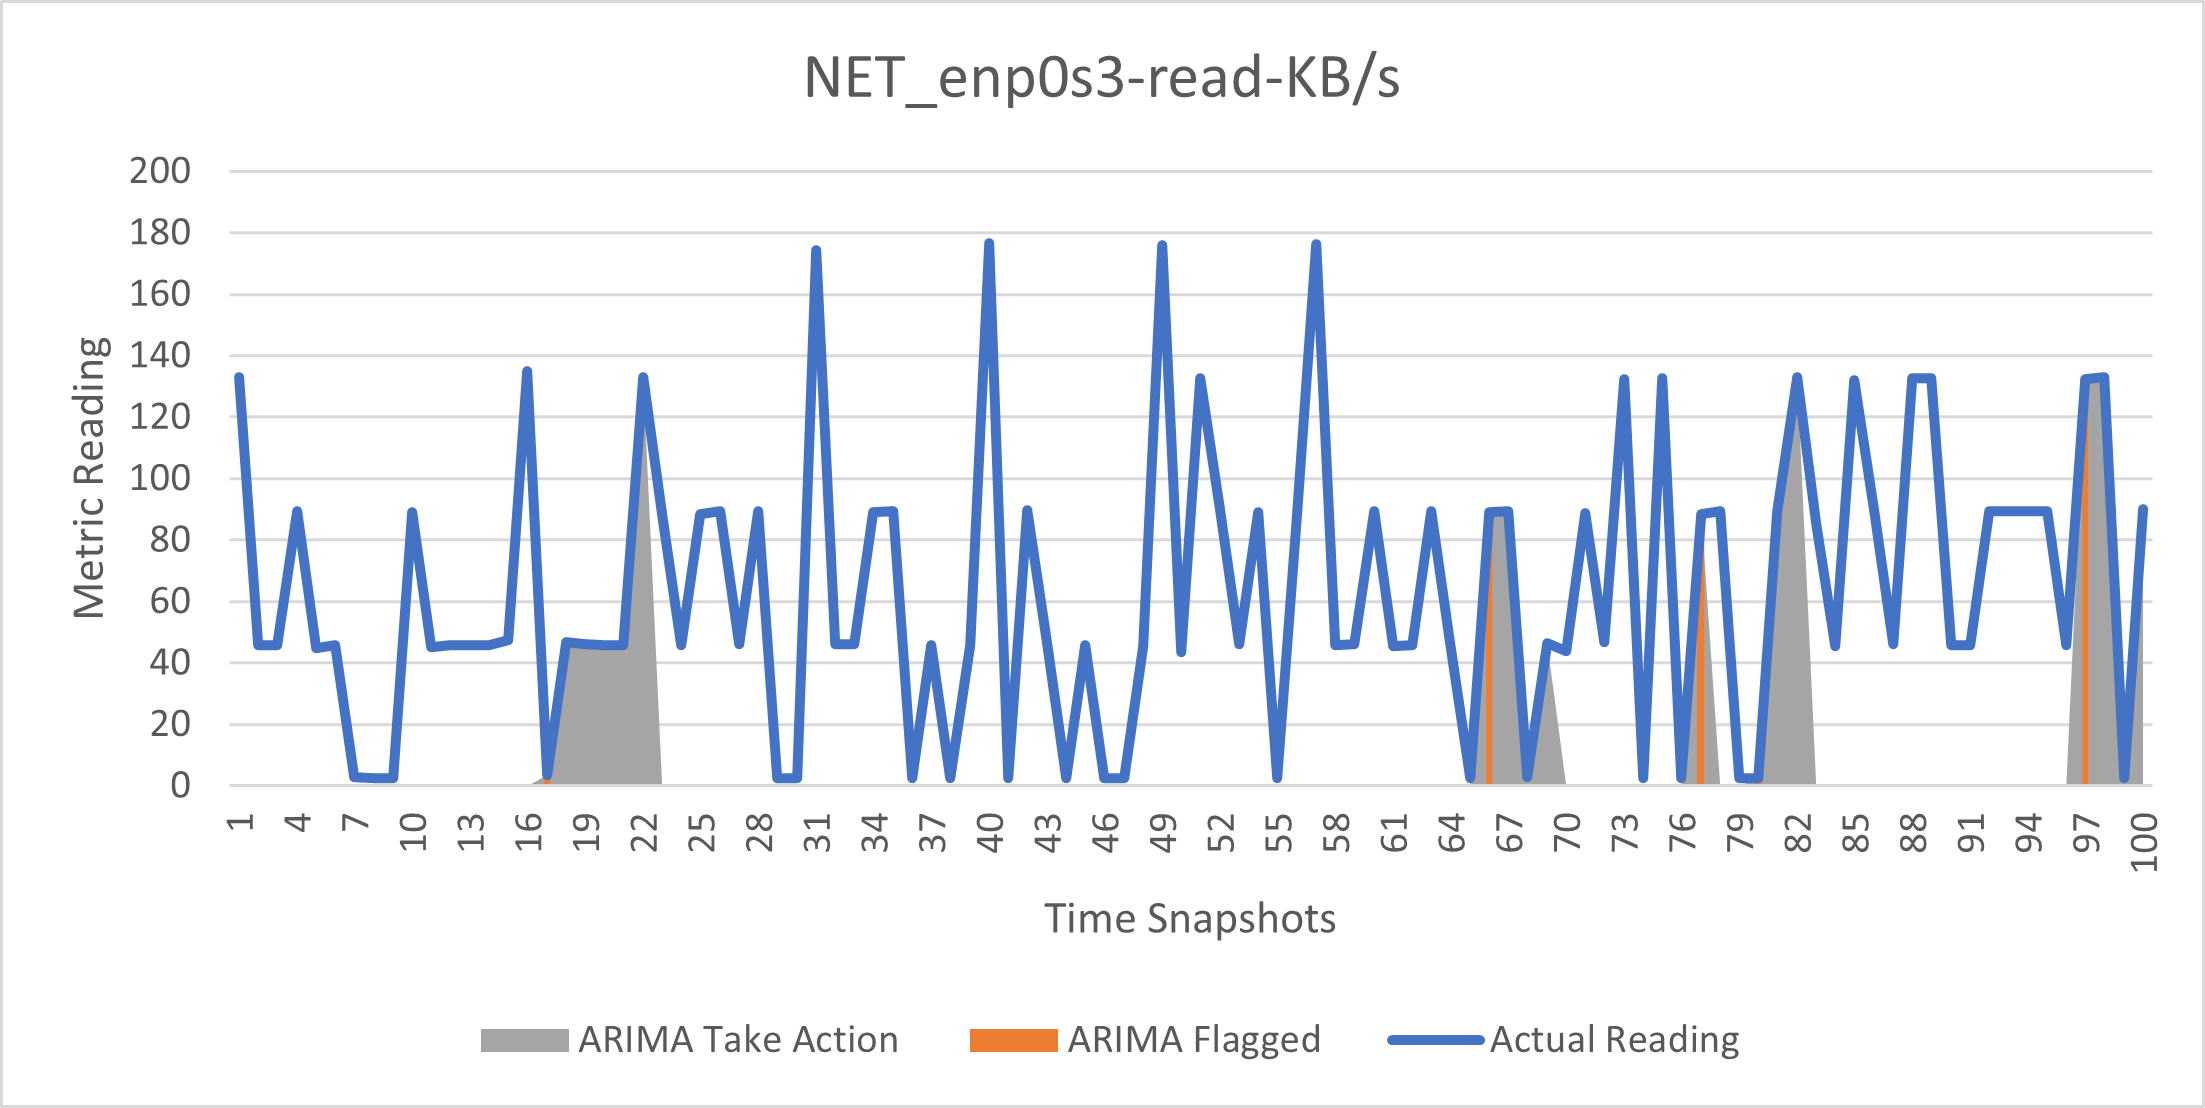
\includegraphics[width=\textwidth]{images/metrics_charts/30_pct_file_load/c1_s1/36.png}
         \caption{NET-read-KB/s | Adaptive Decision}
         \label{fig:c1_s1_36}
     \end{subfigure}
     \hfill
     \begin{subfigure}[ht]{0.32\textwidth}
         \centering
         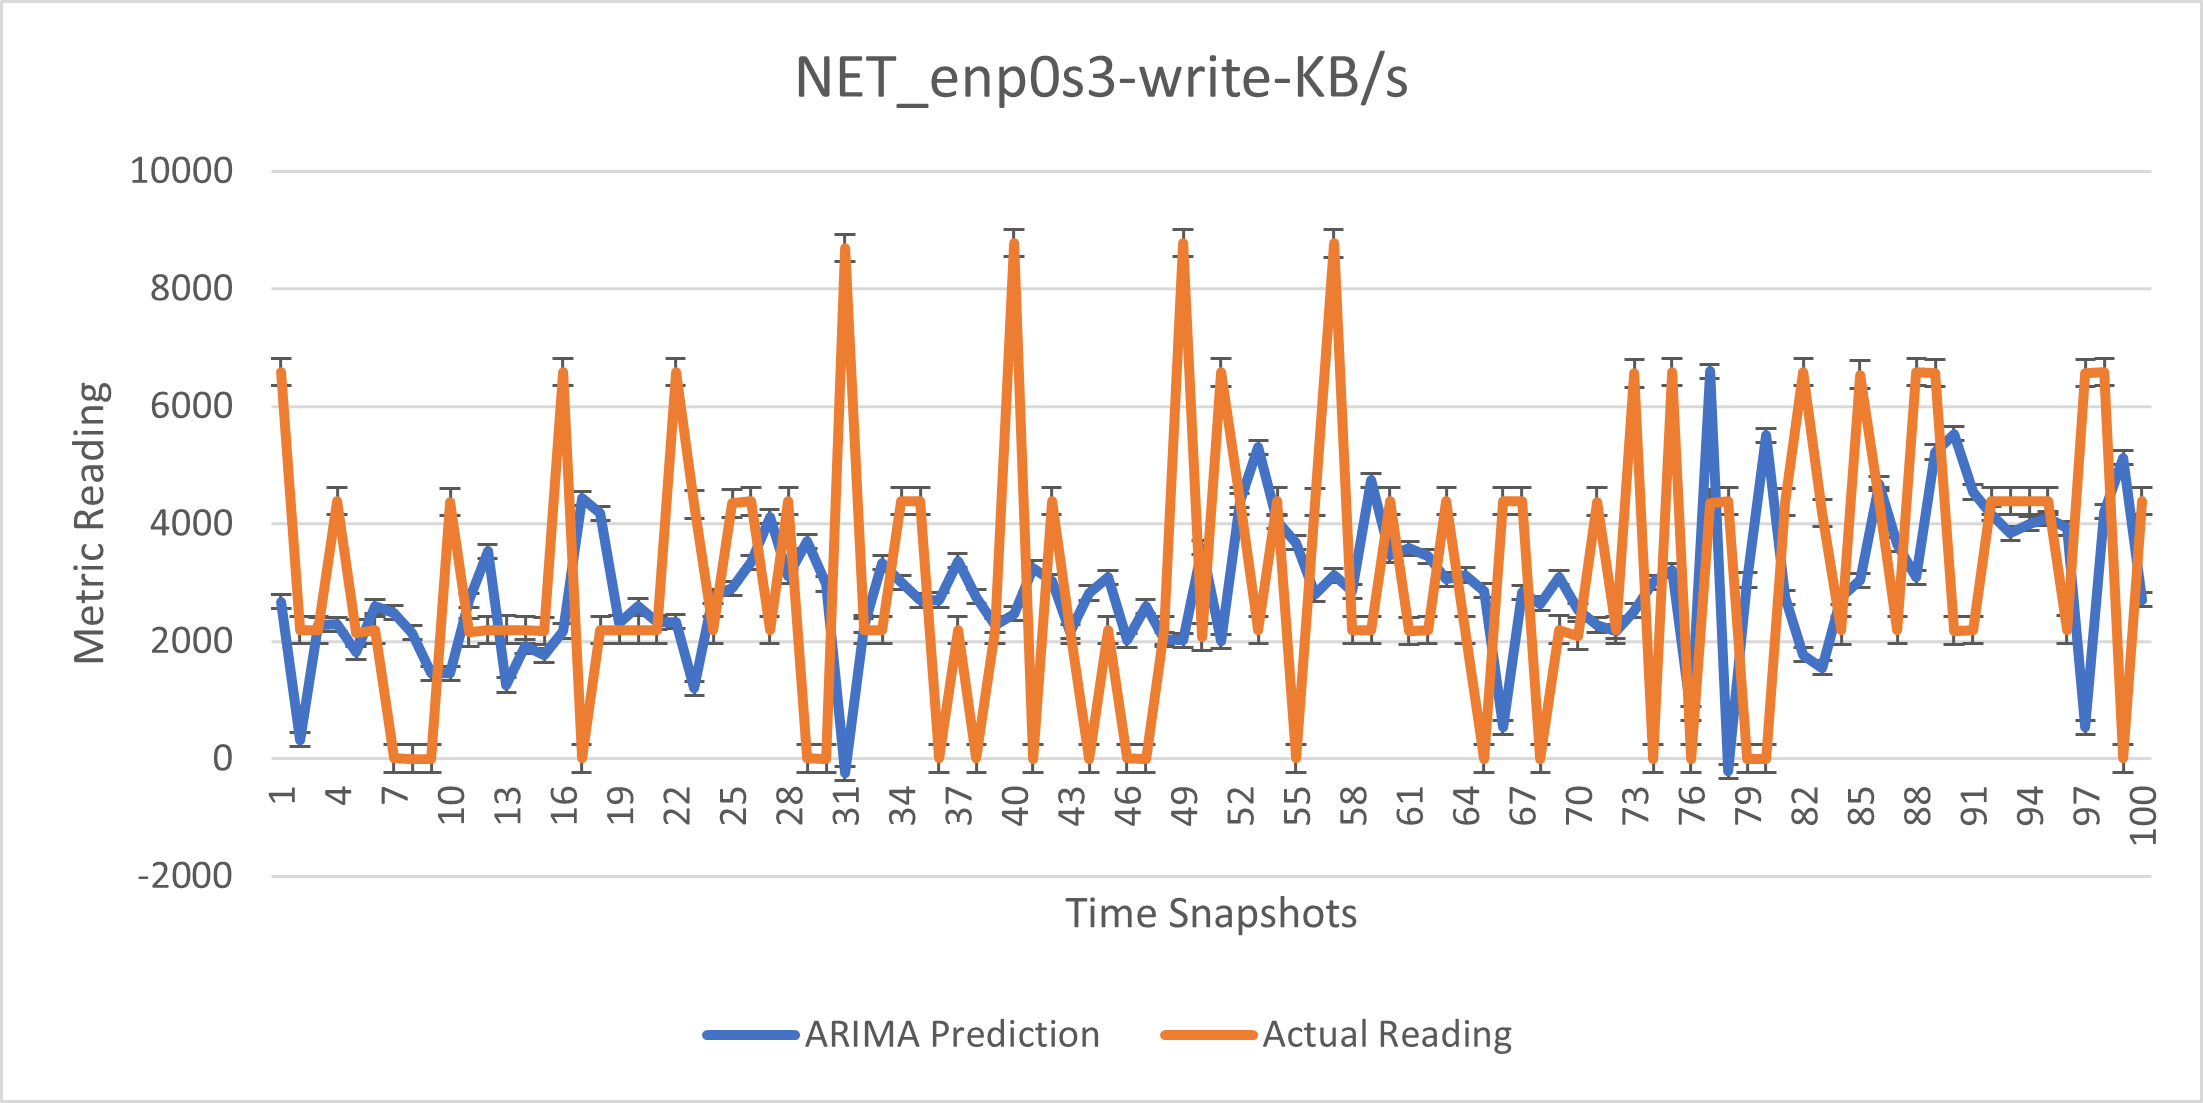
\includegraphics[width=\textwidth]{images/metrics_charts/30_pct_file_load/c1_s1/37.png}
         \caption{NET-write-KB/s | ARIMA Prediction}
         \label{fig:c1_s1_37}
     \end{subfigure}
     \hfill
     \begin{subfigure}[ht]{0.32\textwidth}
         \centering
         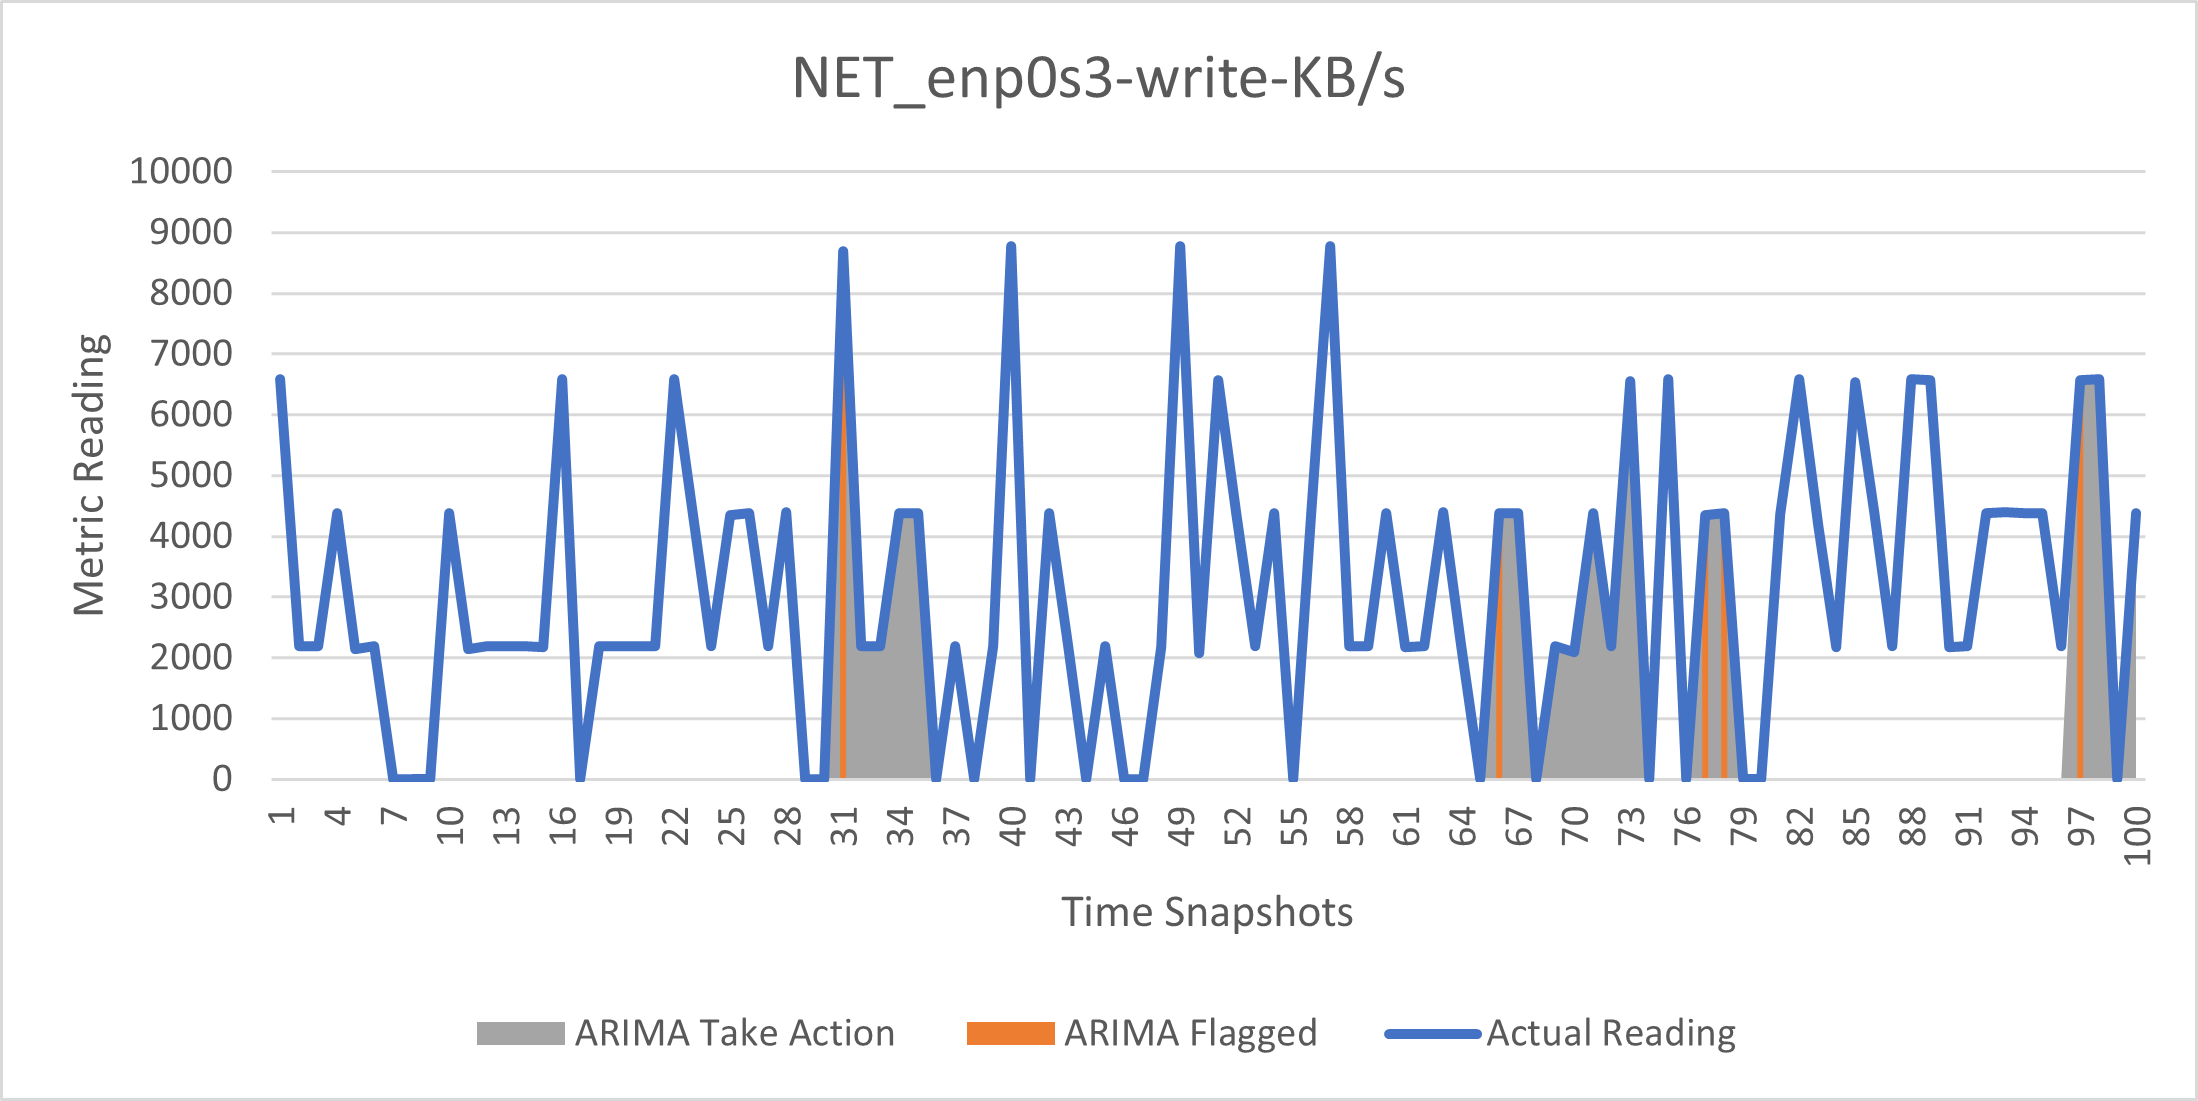
\includegraphics[width=\textwidth]{images/metrics_charts/30_pct_file_load/c1_s1/38.png}
         \caption{NET-write-KB/s | Adaptive Decision}
         \label{fig:c1_s1_38}
     \end{subfigure}
     \hfill
     \begin{subfigure}[ht]{0.32\textwidth}
         \centering
         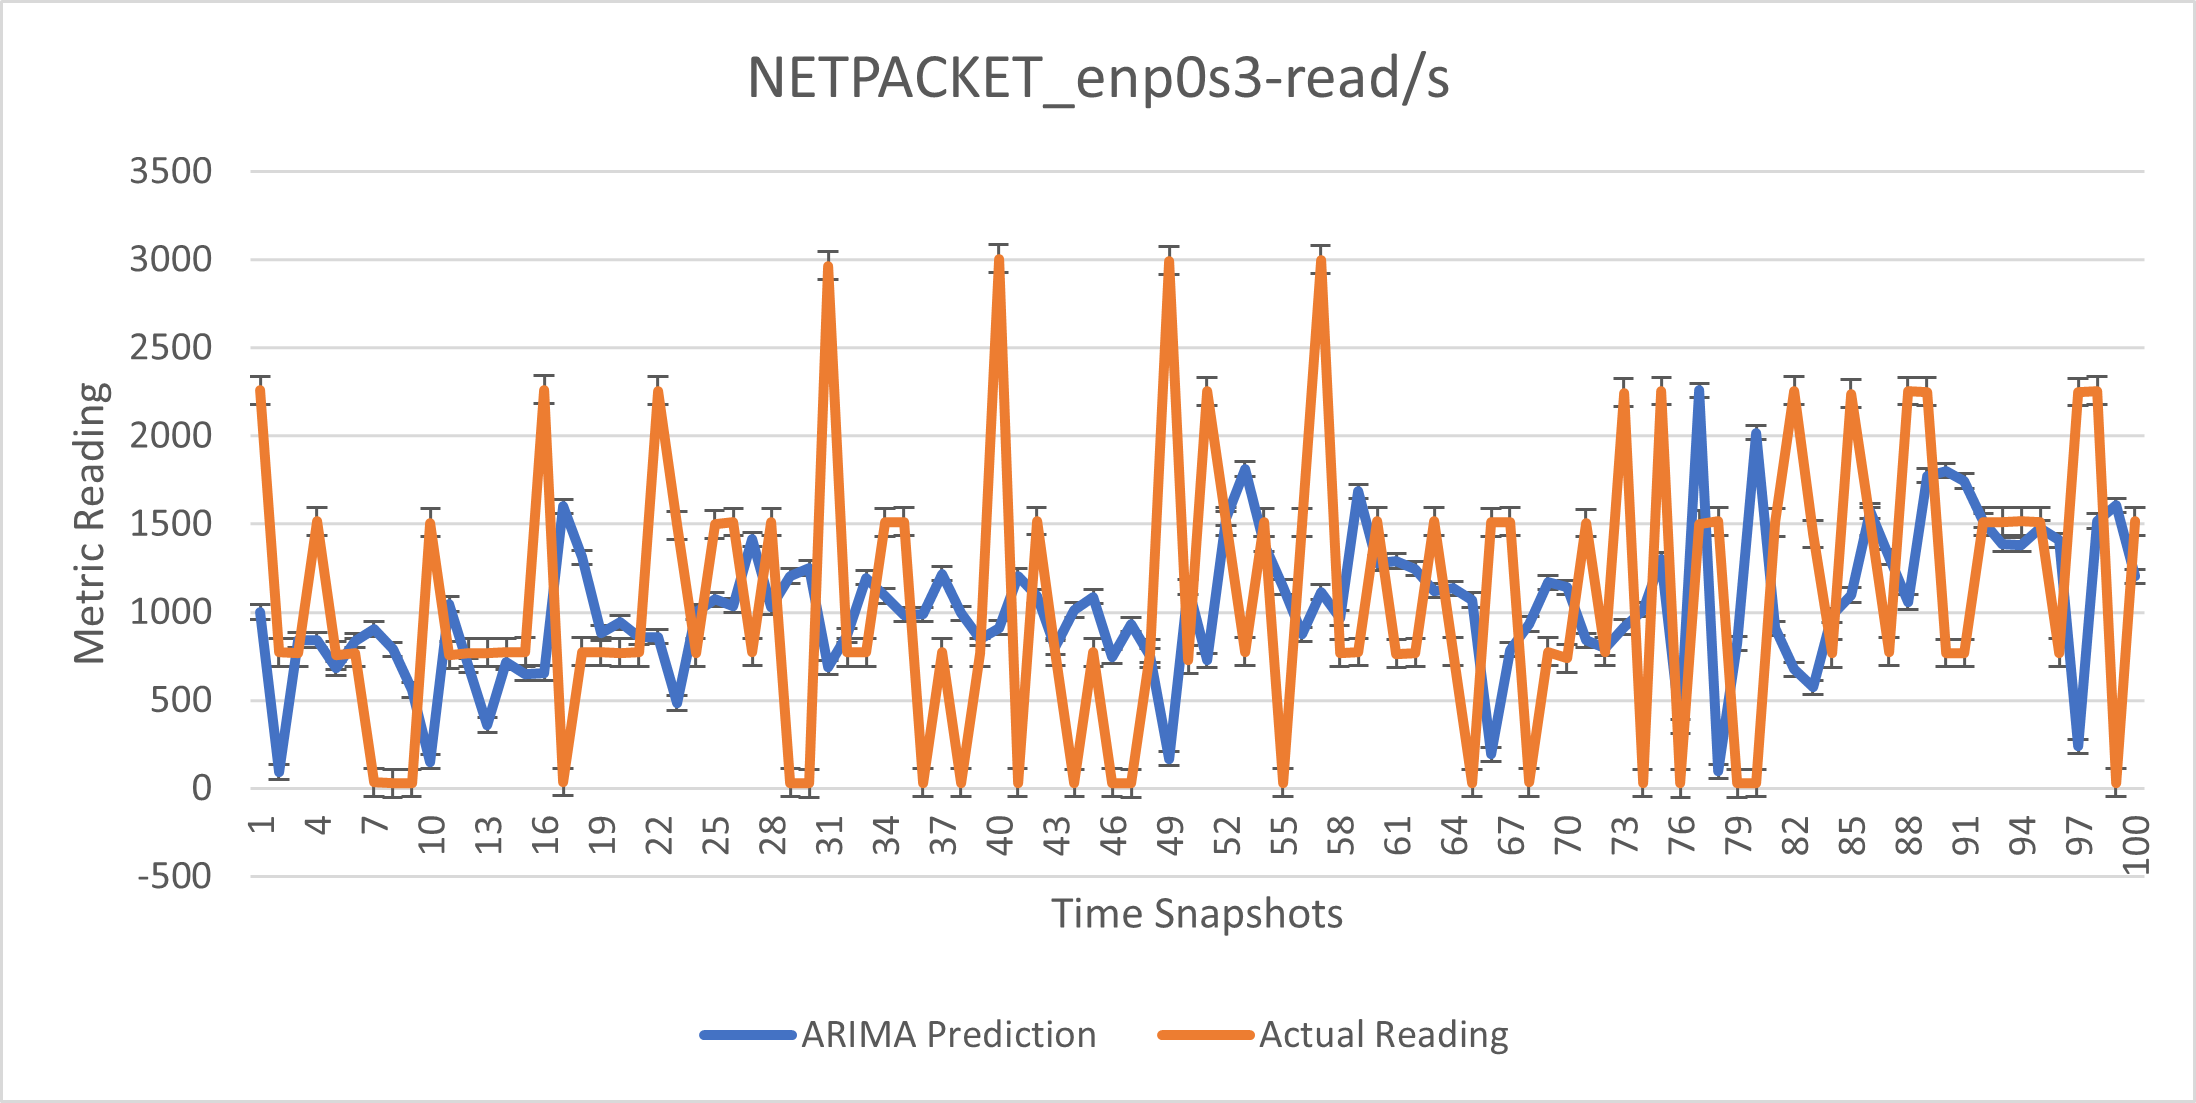
\includegraphics[width=\textwidth]{images/metrics_charts/30_pct_file_load/c1_s1/39.png}
         \caption{NETPACKET-read/s | ARIMA Prediction}
         \label{fig:c1_s1_39}
     \end{subfigure}
     \hfill
     \begin{subfigure}[ht]{0.32\textwidth}
         \centering
         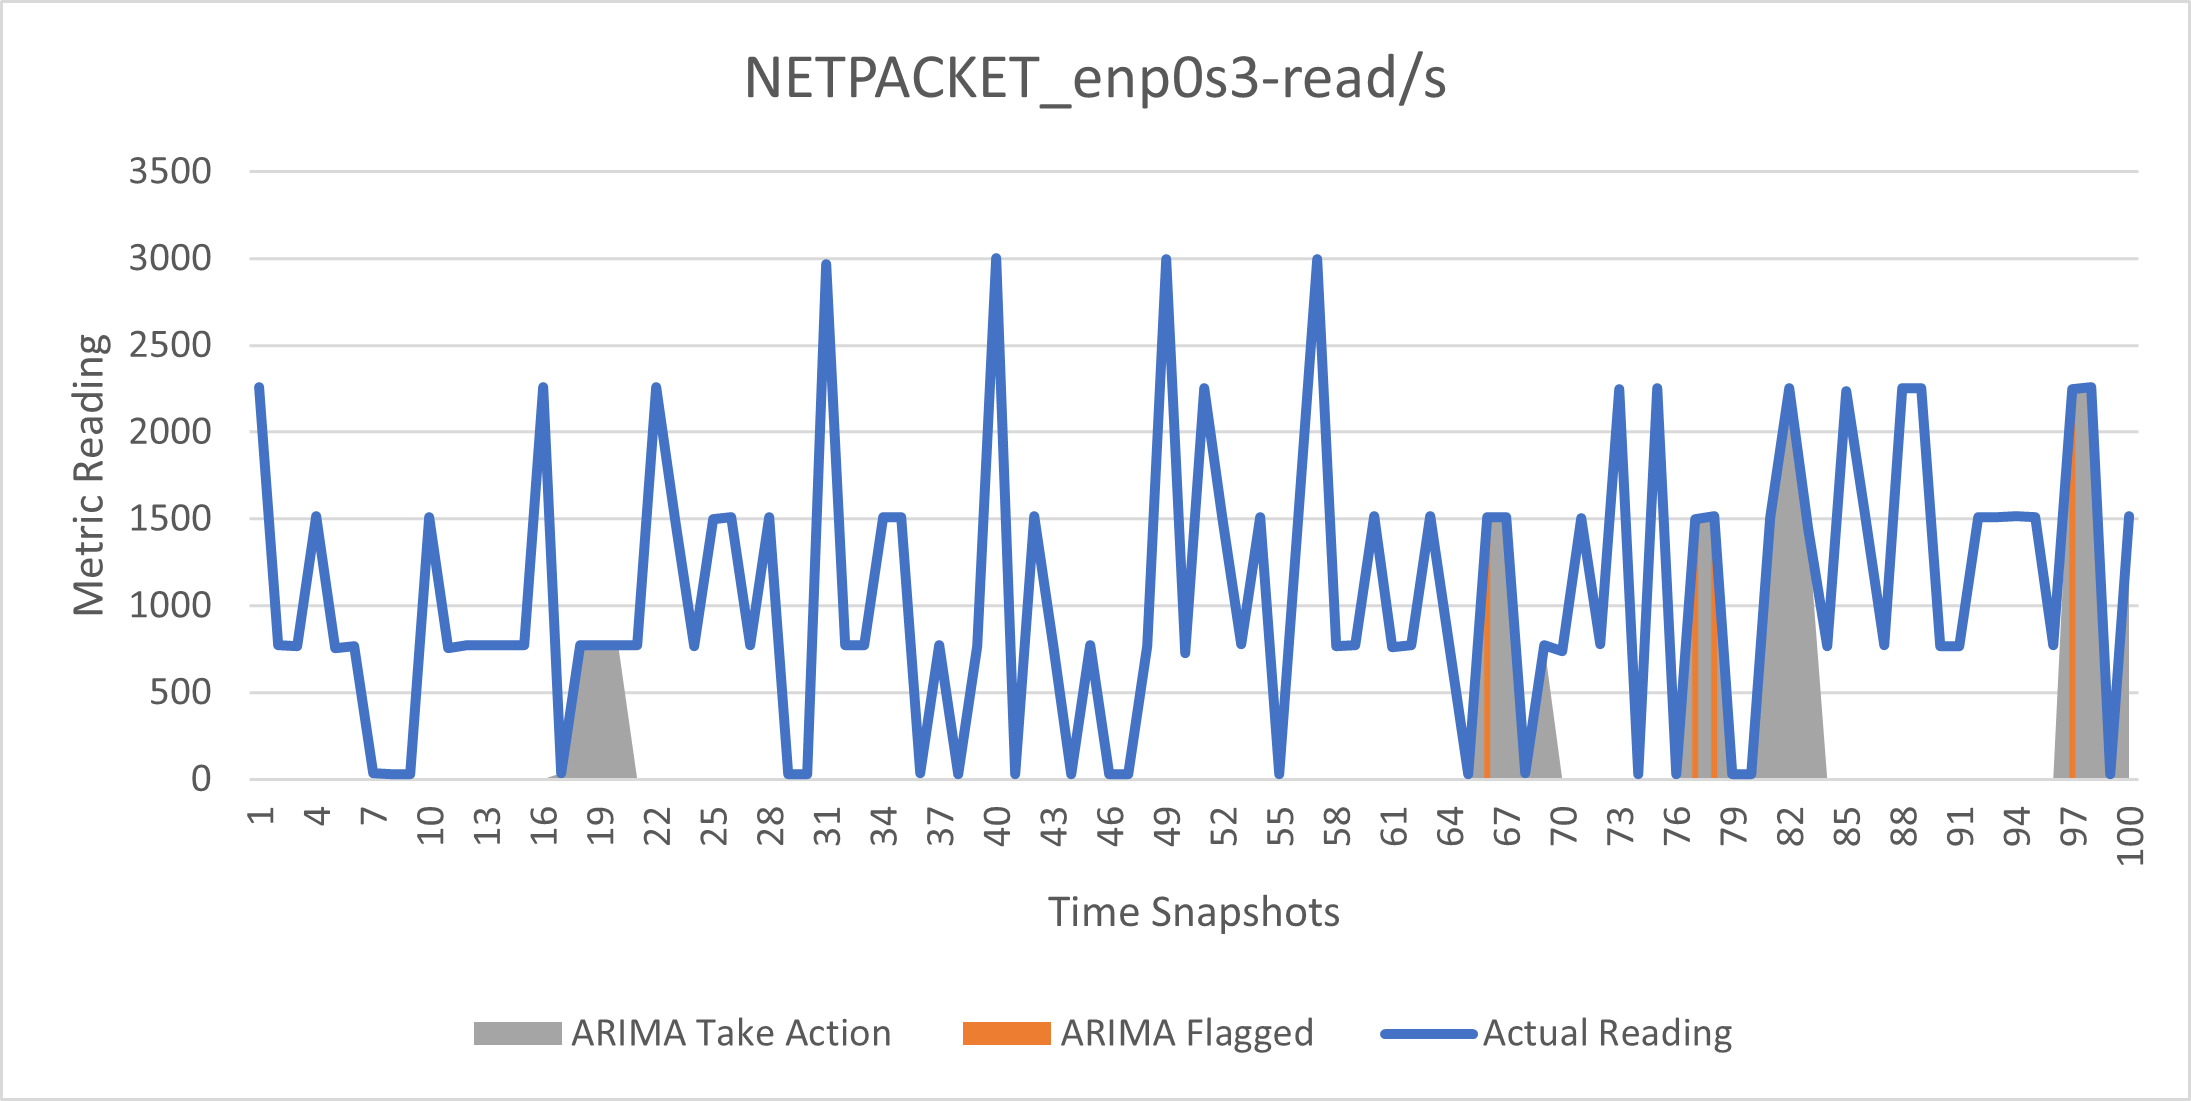
\includegraphics[width=\textwidth]{images/metrics_charts/30_pct_file_load/c1_s1/40.png}
         \caption{NETPACKET-read/s | Adaptive Decision}
         \label{fig:c1_s1_40}
     \end{subfigure}
     \hfill
     \begin{subfigure}[ht]{0.49\textwidth}
         \centering
         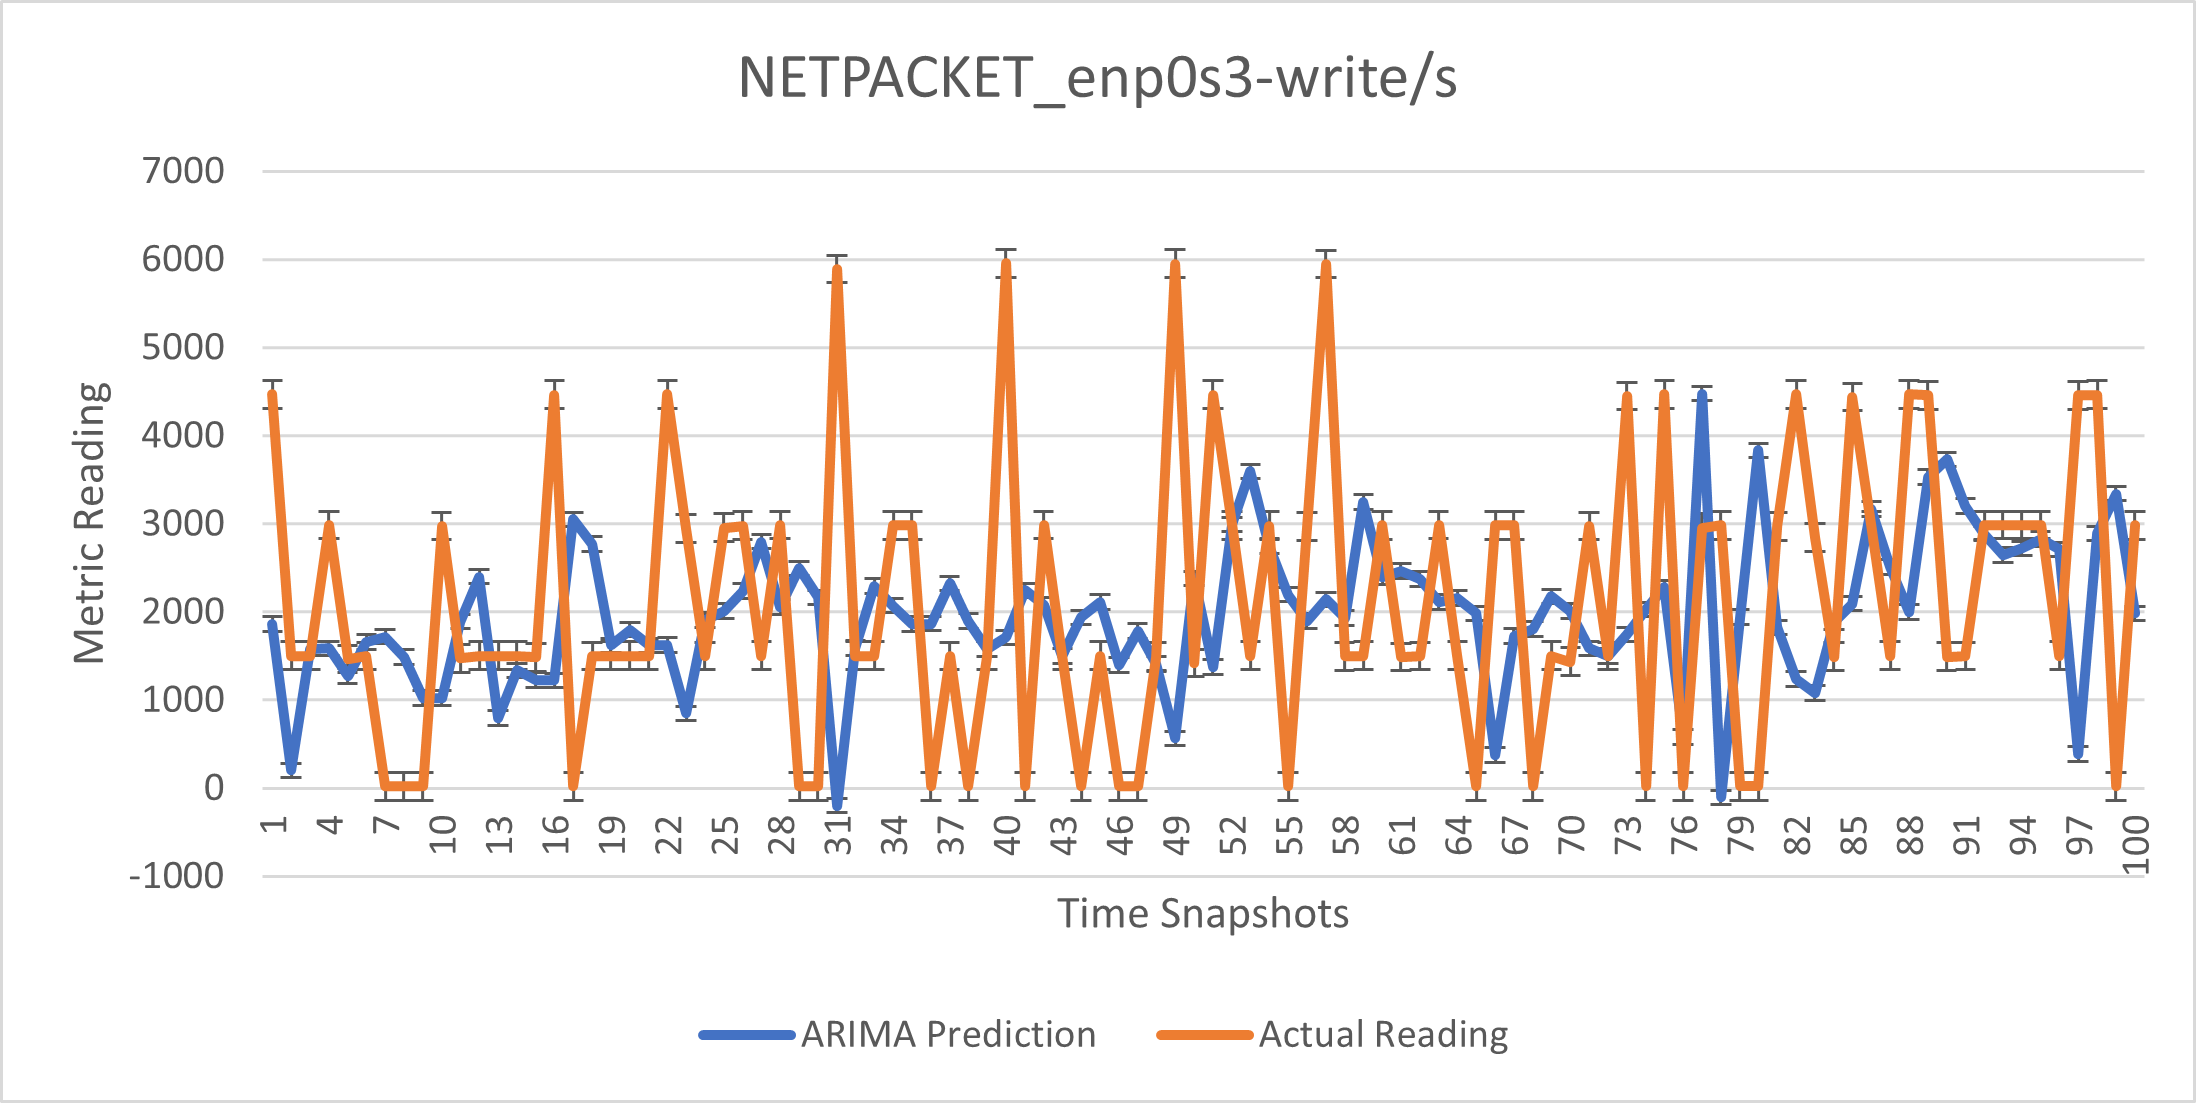
\includegraphics[width=\textwidth]{images/metrics_charts/30_pct_file_load/c1_s1/41.png}
         \caption{NETPACKET-write/s | ARIMA Prediction}
         \label{fig:c1_s1_41}
     \end{subfigure}
     \hfill
     \begin{subfigure}[ht]{0.49\textwidth}
         \centering
         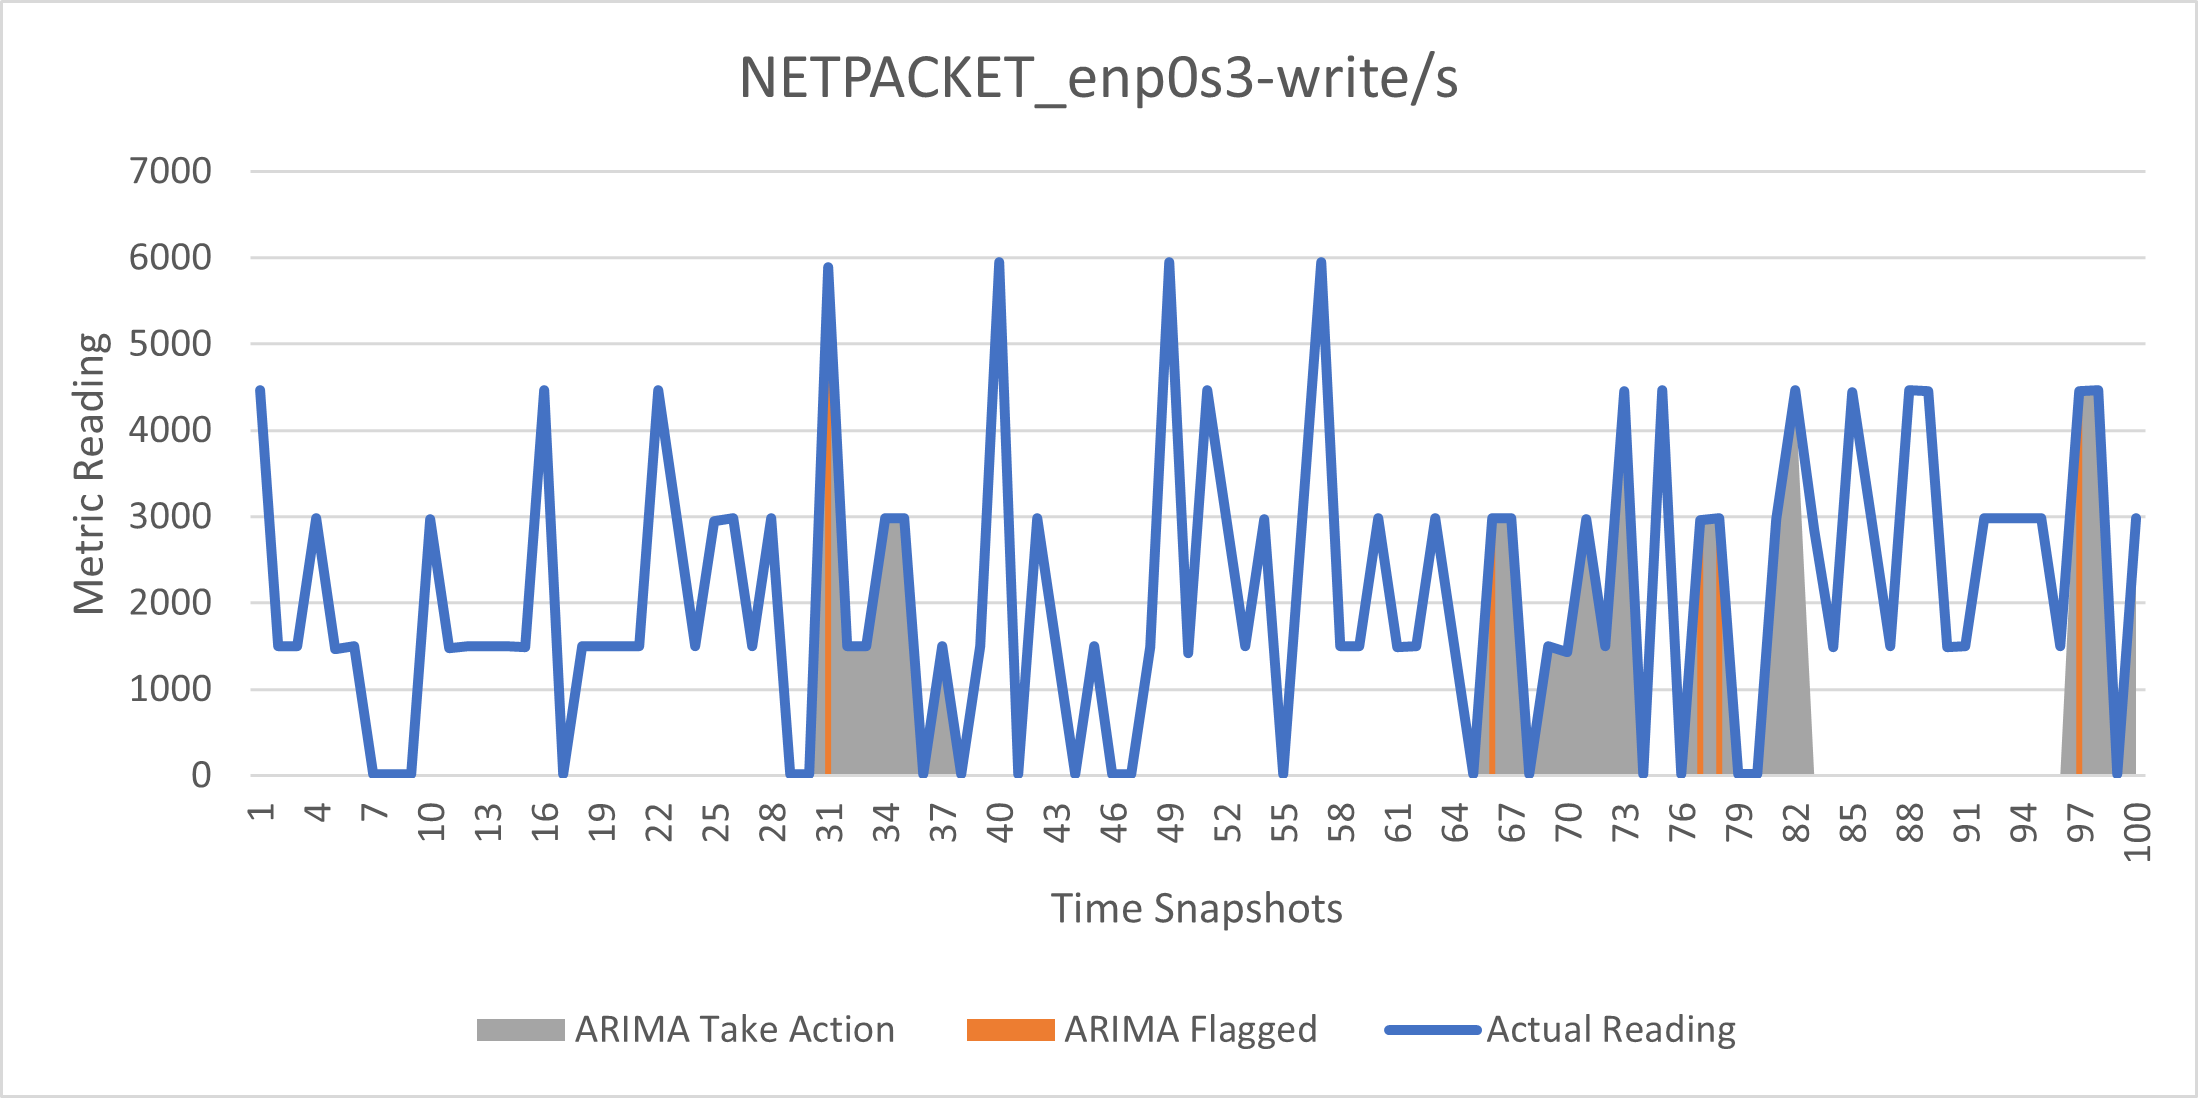
\includegraphics[width=\textwidth]{images/metrics_charts/30_pct_file_load/c1_s1/42.png}
         \caption{NETPACKET-write/s | Adaptive Decision}
         \label{fig:c1_s1_42}
     \end{subfigure}
     \hfill
     
     \caption{Network Metrics For Interface Enp0s3 | Case Study: 1}
     \label{fig:c1_s1_network}
\end{figure*}


\subsubsection{Overhead}\label{case studies & evaluation: evaluation case study 1}
For evaluating the performance of our approach in this case study, we focus on two key aspects: runtime overhead and the effectiveness of metric selection. Since ARIMA models can be executed on a separate machine, the primary overhead on the production system comes from nmon's CPU utilization. To quantify the runtime overhead, we compared CPU utilization snapshots in two distinct settings. In the first setting, nmon was run alongside the Apache server while serving requests. In the second setting, nmon was executed while ignoring metrics discarded during the preliminary monitoring phase, using the same benchmark for both configurations.

Figure \ref{fig: evaluationcs1} shows the chart of CPU utilization with and without nmon recording metrics in the background. It is noted that during this stage, nmon monitored all possible metrics supported by nmon with a sampling rate of 1 second. The overall overhead was observed to be an average of 6.8\% compared to the baseline. However, the baseline itself had a maximum CPU utilization of 9\%. Note that the CPU utilization for nmon remains static unless the sampling rate changes. Therefore, it is safe to assume that the overhead for nmon would drastically reduce with a higher baseline CPU utilization. Our findings show that nmon added only an additional 0.3\% CPU utilization on average, with the maximum being 0.7\% and the lowest being very close to 0\%.

\begin{figure}[tbp]
    \centering
    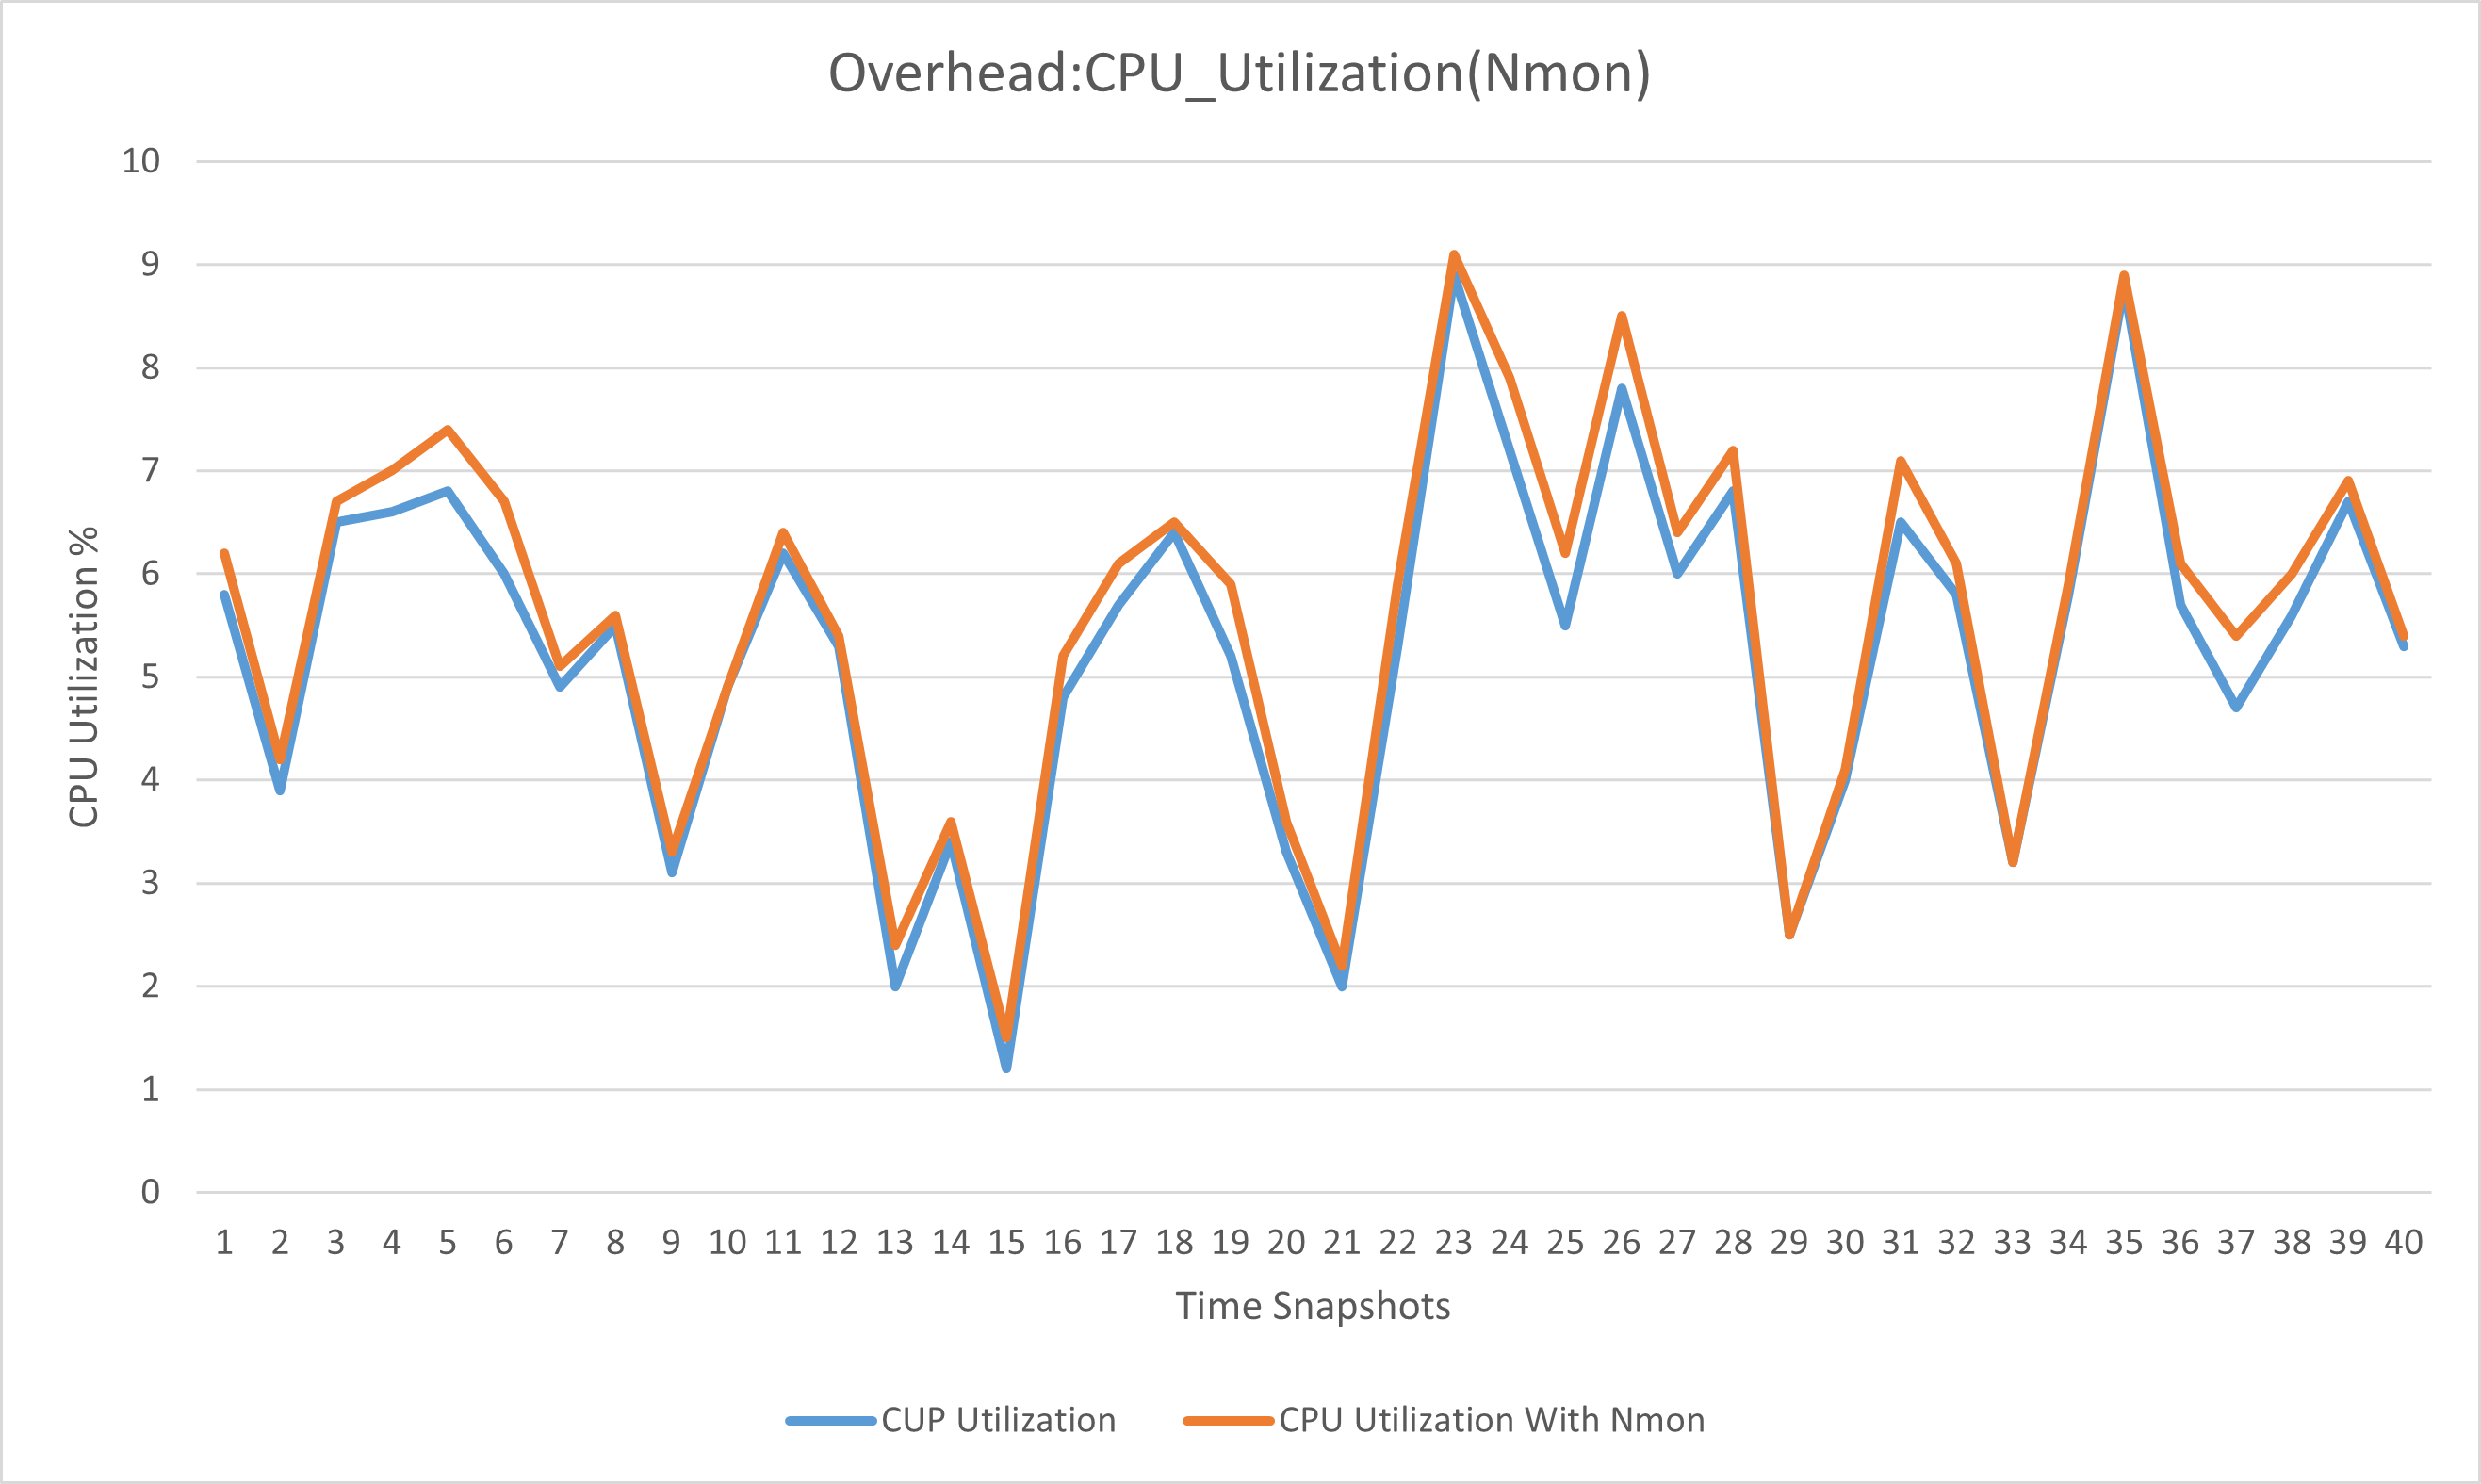
\includegraphics[width=\linewidth]{images/evaluation/cs1/c1_1.png}
    \caption{Overhead Analysis of Case Study 1.}
    \label{fig: evaluationcs1}
\end{figure}

Figure \ref{fig: evaluationcs2} shows the comparison of overhead between the base model of nmon with all metrics being recorded against nmon with selective metrics set after the preliminary monitoring stage. While comparing against the base model, we can observe that the selective metrics model has an average of 4.3\% overhead reduction with respect to the whole system's utilization. Further analyzing the CPU utilization, we can observe that the selective metrics model saves an average of 0.2\% CPU utilization compared to the base model. This 0.2\% reduction is a 66\% overhead improvement if compared against the 0.3\% average CPU utilization of the base model alone.


\begin{figure}[tbp]
    \centering
    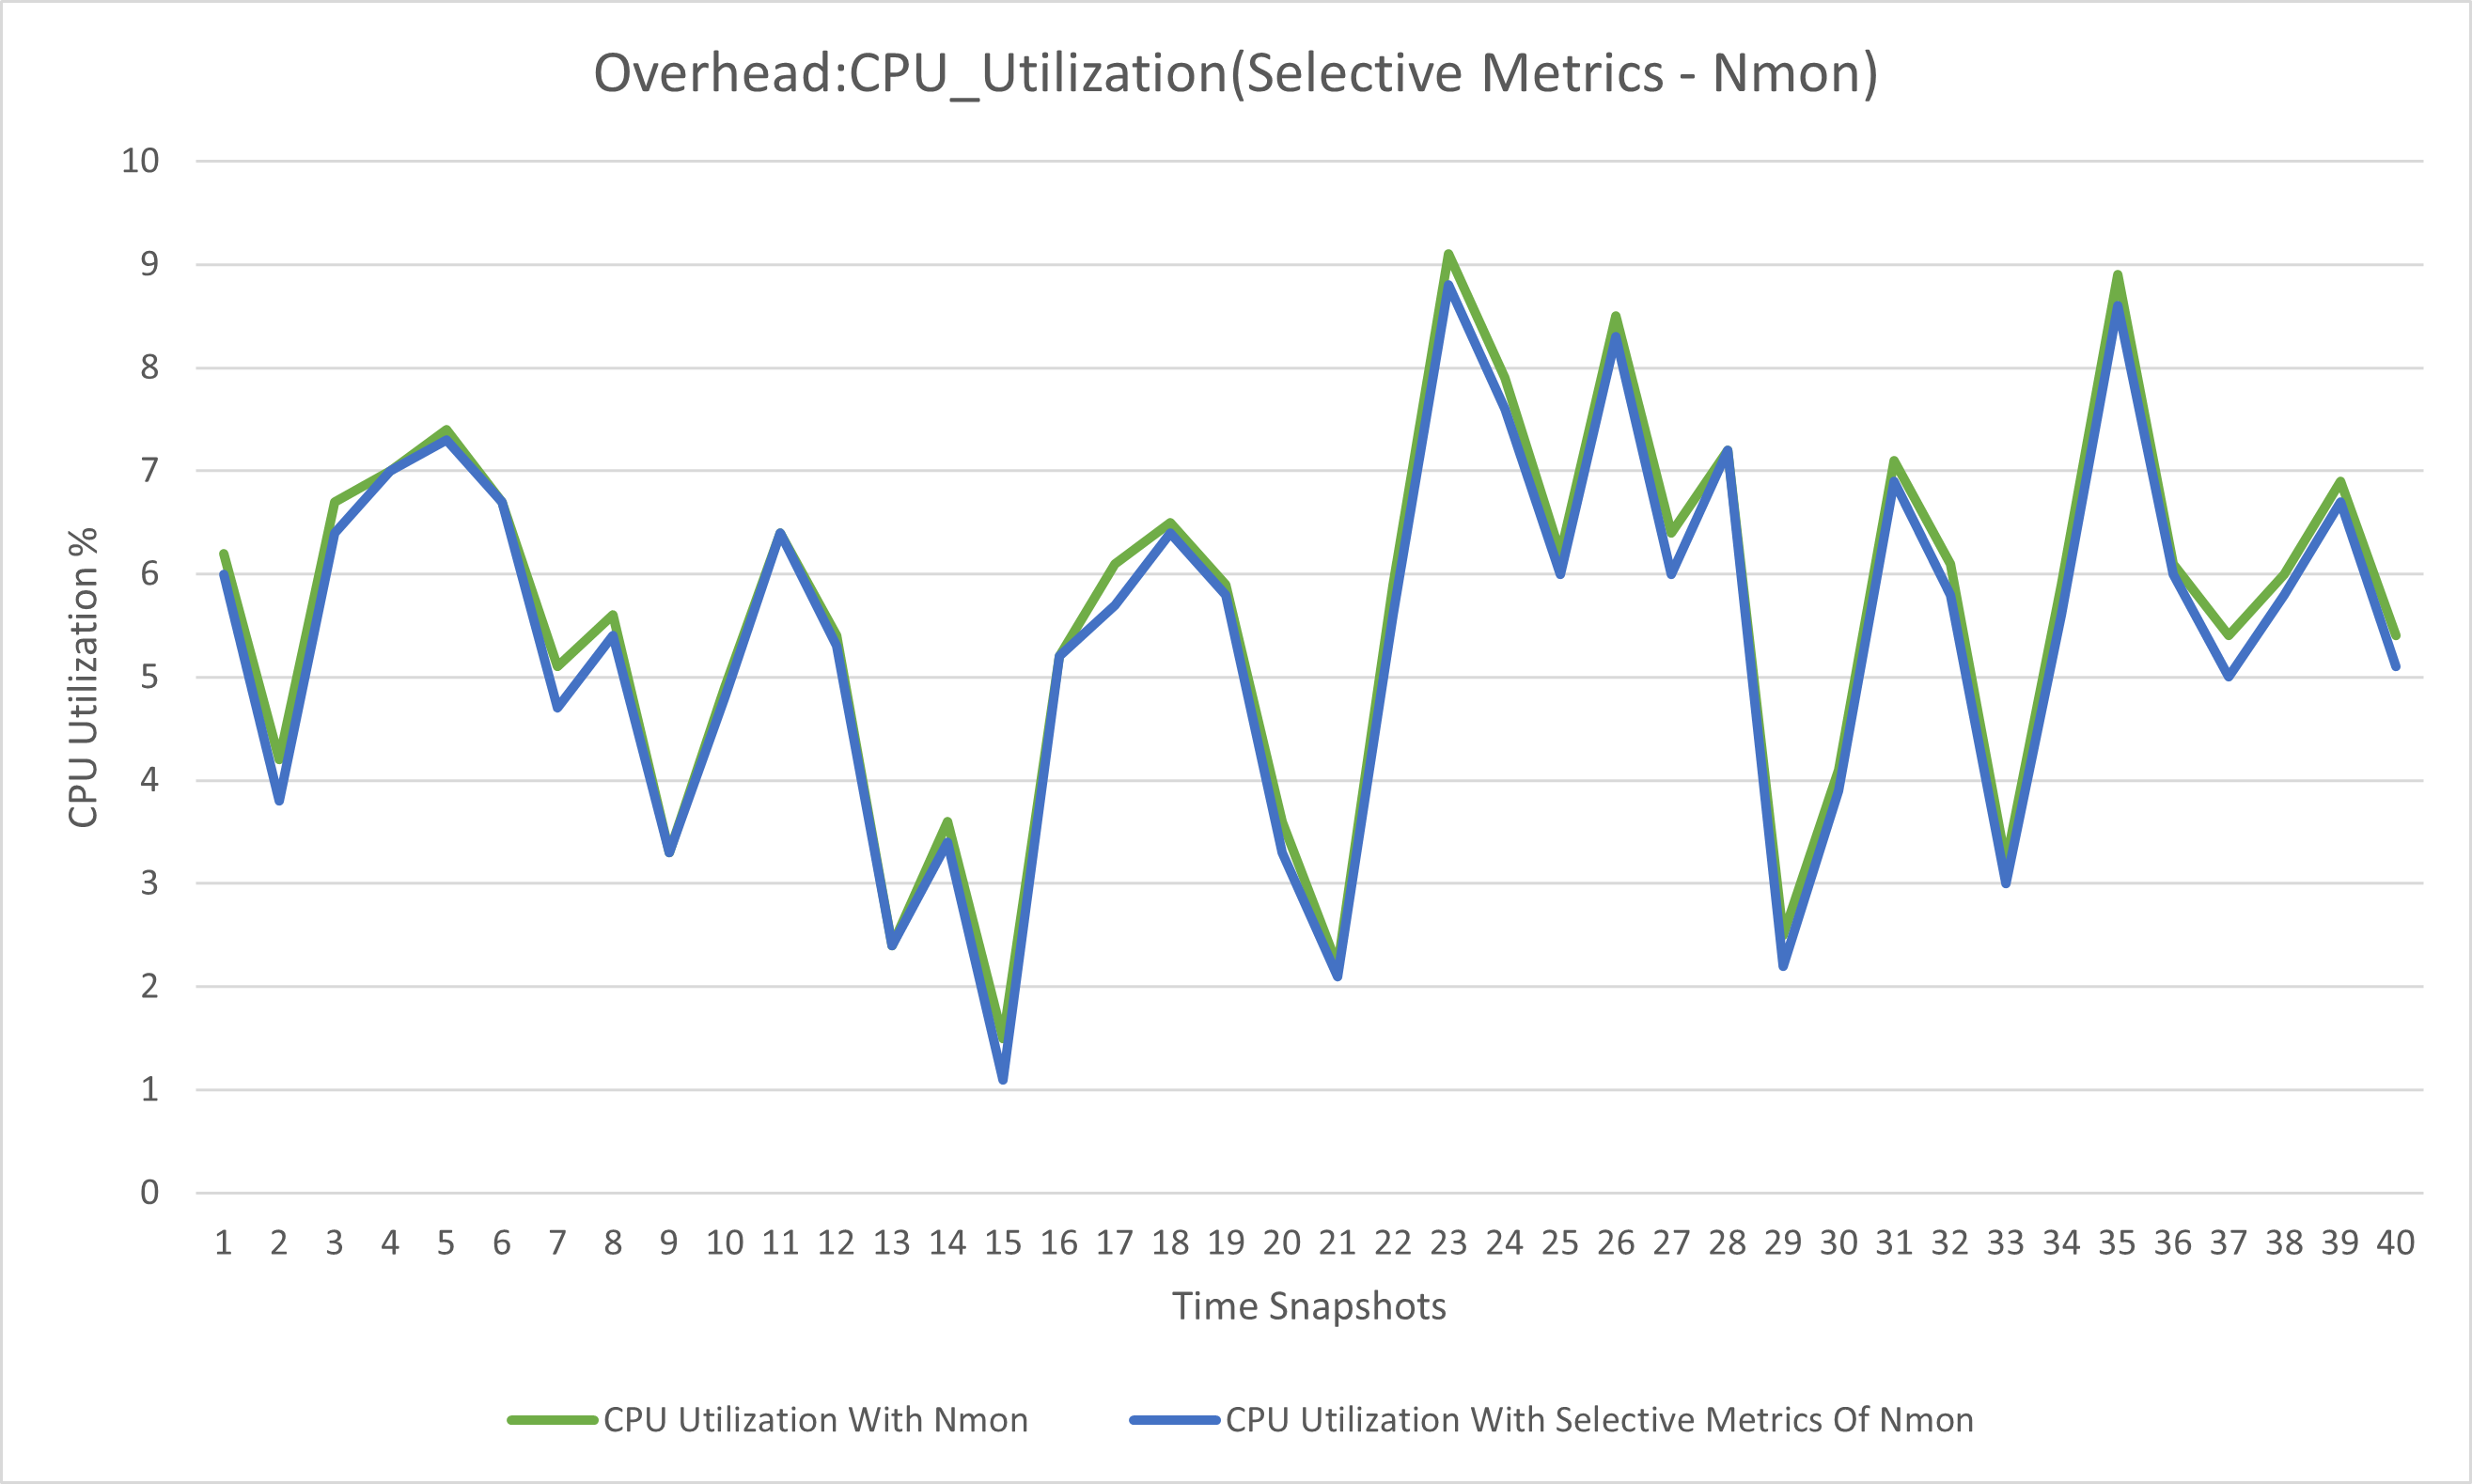
\includegraphics[width=\linewidth]{images/evaluation/cs1/c1_2_2.png}
    \caption{Evaluation | Overhead Comparison With Selective Metrics | Case Study: 1}
    \label{fig: evaluationcs2}
\end{figure}

\subsection{Case Study \#2}\label{case studies & evaluation: case study 2}


This case study was performed on the Firefox web browser, a complex multi-threaded application. The case study was an analysis from a Bugzilla report \cite{clessili-2022}, which stated that Firefox takes a long time loading larger PDF files even if it is locally stored. The report mentioned that Firefox gets stuck for a while at a function call responsible for handling the graphic driver. The mentioned function call is related to VSync, which synchronizes the refresh rate between the monitor screen and the graphic processor. Therefore, it was concluded that Firefox has an issue with the function-call responsible for calling the driver for VSync. 

% \subsubsection{Goal Of This Case Study}

% This case study aims to demonstrate if our method can detect performance issues caused by driver-related communication between applications and hardware. We have demonstrated how our method has reacted to this issue upon reproducing it and what adaptive tracing suggestions would have been provided.


\subsubsection{Data Collection}\label{case studies & evaluation: data collection case study 2}

To create the tracing profile, we have selected a 50 MB PDF file and a 500kb PDF file. Next, Firefox was built from source by enabling the perf flag so that JIT can be profiled by following the instructions from Mozilla's documentation on Firefox \cite{firefoxdocumentation}.
Firefox was continuously loaded with the larger and smaller PDFs in various combinations to explore all possible function calls and system calls for loading PDFs in Firefox. This load and stress test was carried out for 20 minutes. Once the Firefox build is ready, we used perf for recording the call stacks as explained in section~\ref{Pre-Testing and Methods Selection} to build up the tracing profile.

Next, the family-groups of the functions and system calls were identified and sorted based on the priority of importance as explained in Algorithm \ref{familygroup}. For calculating the execution time of the function calls, we have used a split of ten-millisecond snapshots while recording call stacks with perf. The ten milliseconds were used as the time snapshot. Once the execution time for each function and system calls were found, we then passed those values into Algorithm \ref{covranking} to get them ranked. For our experiment, we used a functions and system calls list cutoff value of 5\% of the total number of function and system calls discovered.

We found a total of 8,231 unique family-groups for both function and system calls combined. The selected list had a total of 410 function and system calls. Selecting 5\% of the functions to be monitored may sound like a lot of important data may be missed. However, it must be reminded again that as explained in section~\ref{cutoffsec} that we have already concluded that consistently worst-performing functions have already been handled in the testing phase, as well as the list has been sorted based on the number of calls (i.e., the importance of the function compared to the overall system), followed by CoV ranking. Therefore, we are already following the most important family-groups, which can cause the highest performance problems.


\subsubsection{Change Detection}\label{case studies & evaluation: change detection case study 2}

To illustrate the framework's behaviour on the known performance issue, we reproduced the scenario described in the Bugzilla report~\cite{clessili-2022}. The function \textquote{$mozilla::VsyncRefreshDriverTimer::RunRefreshDrivers$}, which the report identifies as the culprit, had a ranking of 14 on the monitored candidate list. Firefox used this function call to maintain synchronization between the frame refresh rate of the monitor and Firefox itself to minimize tearing effects when the PDF is scrolled. The framework successfully included this function in the top-5\% monitored set from a total of eight thousand discovered function calls---a substantial overhead reduction compared to tracing all functions.

However, our approach further reduces the overhead by not only specifying which function to trace but also by adaptively deciding \emph{when} to trace the functions. Therefore, not only did it save overhead from tracing all the functions, but it also saved system resources from selectively tracing the functions only when needed.
Figure \ref{fig:c2_1} shows the execution time of the culprit function and its ARIMA predictions. Figure \ref{fig:c2_2} shows the adaptive decisions made on the tracepoint for the culprit function. It clearly shows that there were moments when the execution time for the function took a lot more than 10ms. While loading the smaller PDF, the average time for this function's execution remained well below 20 milliseconds. However, from Figure \ref{fig:c2_1}, we can observe that there were moments with well over 500 millisecond execution time for this function.

\begin{figure*}[tbp]
     \centering
     \begin{subfigure}[ht]{0.49\textwidth}
         \centering
         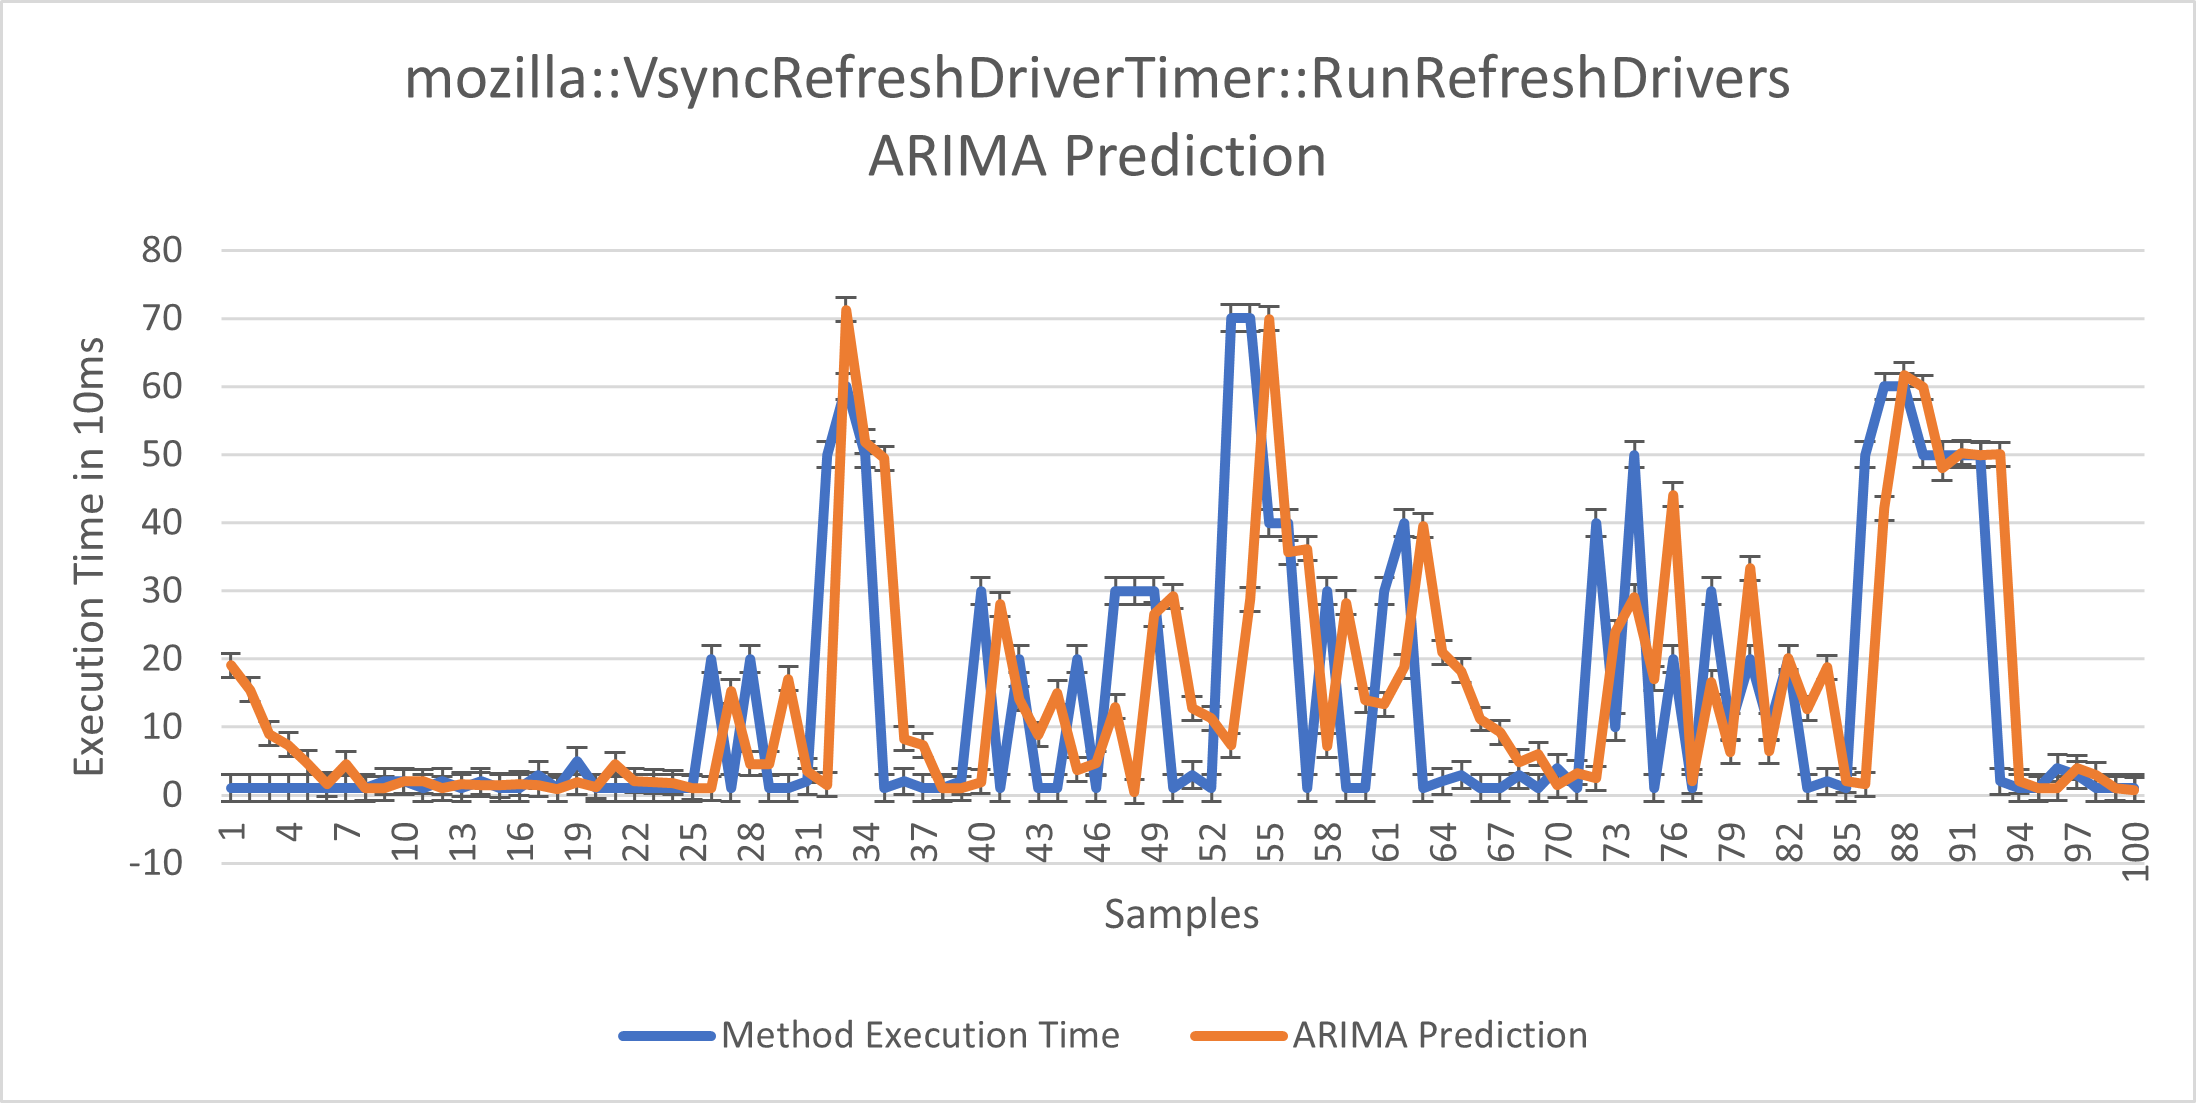
\includegraphics[width=\textwidth]{images/metrics_charts/largepdf/l1.png}
         \caption{Execution Time \& ARIMA Prediction}
         \label{fig:c2_1}
     \end{subfigure}
     \hfill
     \begin{subfigure}[ht]{0.49\textwidth}
         \centering
         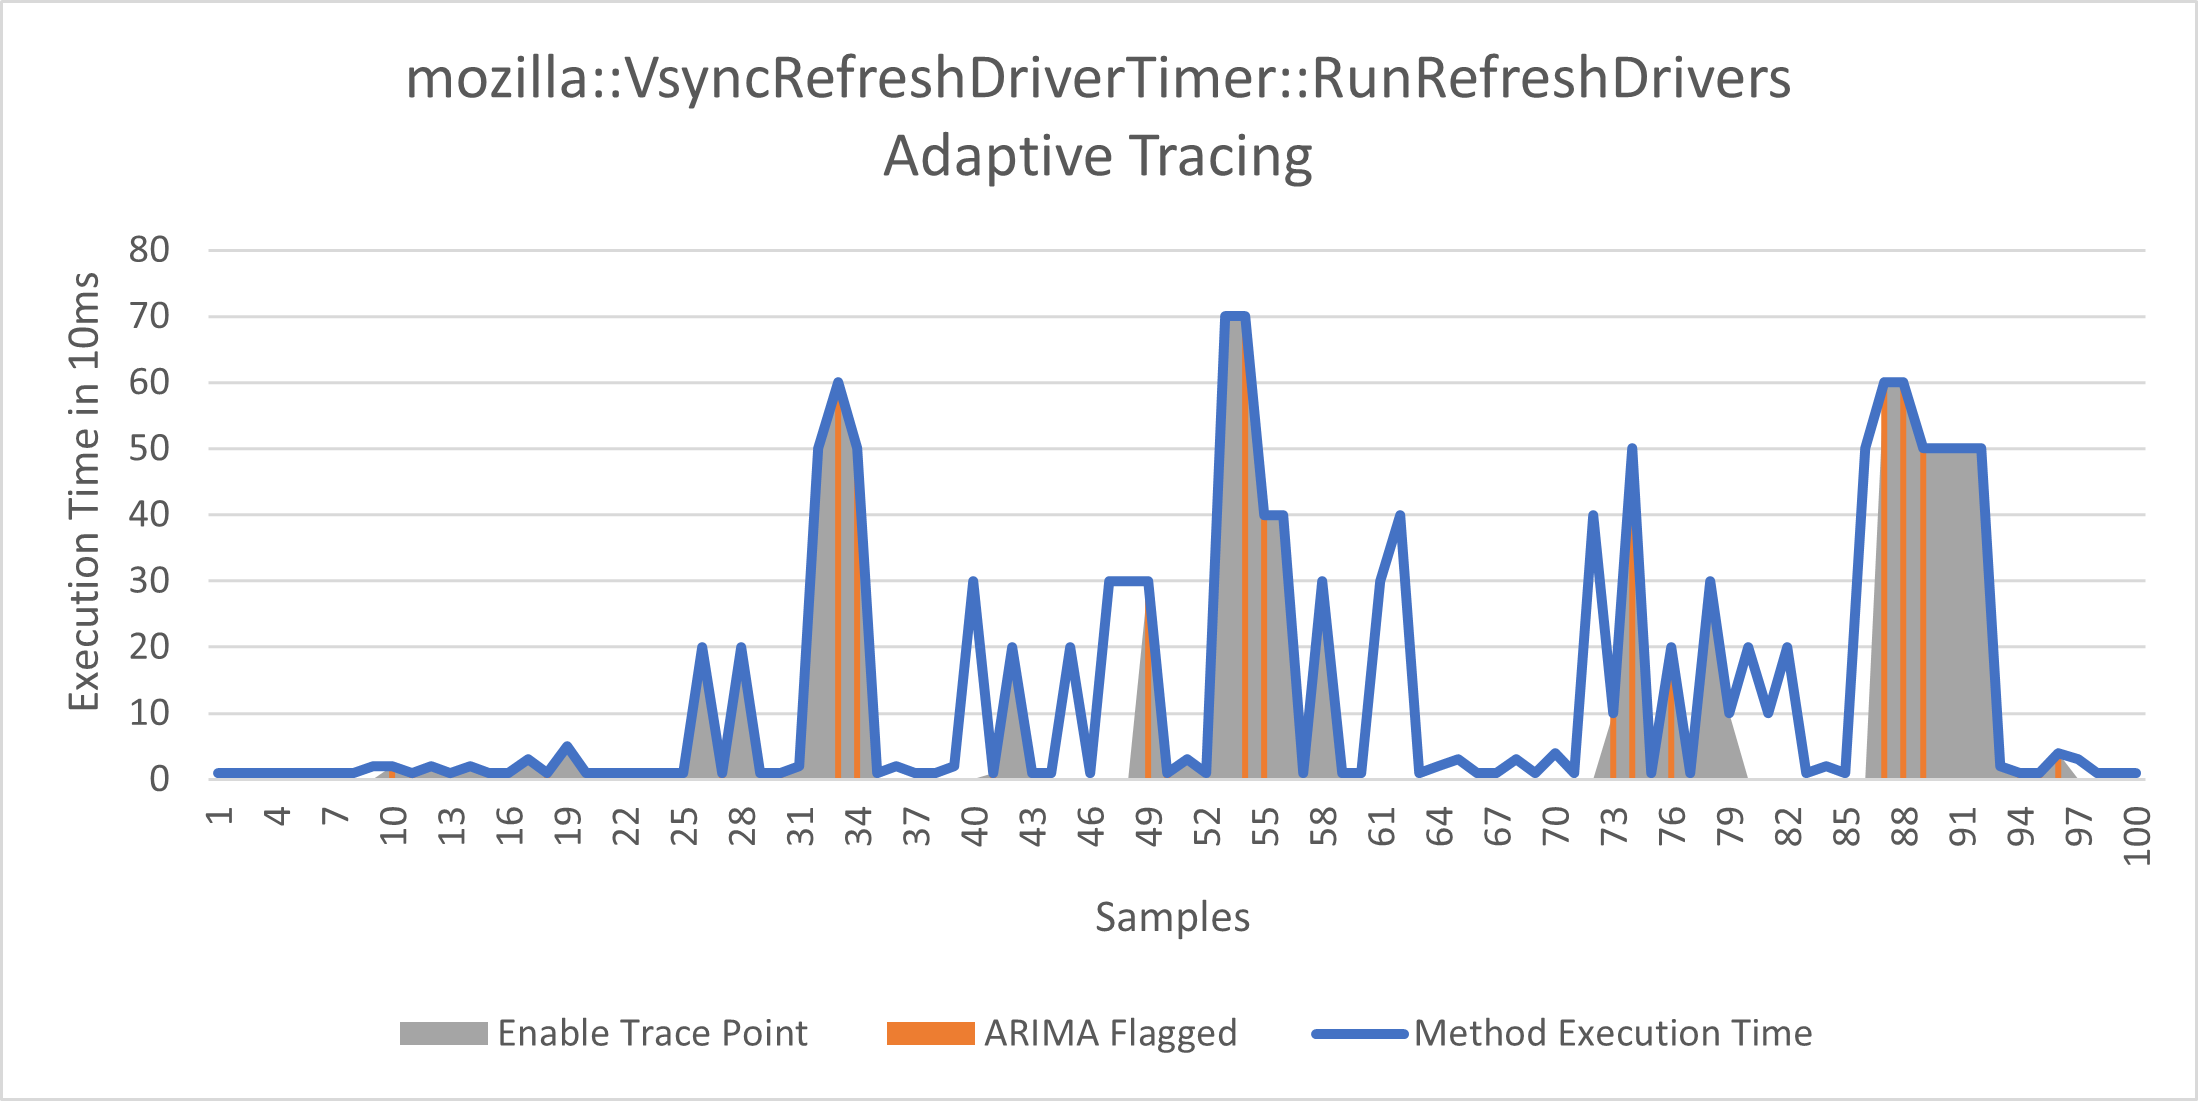
\includegraphics[width=\textwidth]{images/metrics_charts/largepdf/l2.png}
         \caption{Adaptive Decision For Tracepoint}
         \label{fig:c2_2}
     \end{subfigure}
     \hfill
     \caption{Function Call Execution Time \& Adaptive Tracing | Case Study: 2}
     \label{fig:c2_0}
\end{figure*}




\subsubsection{Evaluation}\label{case studies & evaluation: evaluation case study 2}

The primary claim in this case study is that the monitored candidate list includes the known culprit function, and that ARIMA-driven anomaly scoring correctly identifies the time windows when the function exhibits anomalous execution times. Because the candidate list is generated from workload profiling rather than from the bug report, the detection itself is not circular: the framework had no prior knowledge of which specific function would be problematic. The overhead analysis focuses on the monitoring phase: since ARIMA models can be executed on a separate machine, the primary overhead on the production system is the tracing and storage footprint. Since it takes as little as 158~nanoseconds to materialize an LTTng tracepoint \cite{gebai-2018}, the cost of maintaining 410 instrumented points is low in absolute terms. More significantly, the ARIMA-driven decision mechanism reduced the fraction of test time for which the culprit tracepoint was actively recording by 44\%, compared to always-on tracing; this directly reduces the volume of trace data that must be stored and analyzed. It should be noted that the 158~ns figure represents the tracepoint materialization cost in isolation and does not capture end-to-end pipeline overhead (storage I/O, analysis latency) under high concurrency, which remains a direction for future characterization. Table~\ref{tableevaluationcs21} summarises the key evaluation criteria for this case study. 


\begin{table}[tbp]

\centering
\resizebox{\columnwidth}{!}{%
\begin{tabular}{ |l|c| }
\hline
\textbf{Evaluation Criteria} & \textbf{Values} \\
\hline
Was The Bug Detected? & Yes \\
\hline
Culprit Function & mozilla::VsyncRefreshDriverTimer::RunRefreshDrivers \\
\hline
Useful Unique Changes Detected & 22 \\
\hline
Samples Recorded & 56 \\
\hline
Monitoring Overhead Reduced By CoV Ranking & 95\% \\
\hline
Storage Overhead Reduced By ARIMA For Culprit Tracepoint & 44\% \\
\hline
\end{tabular}%
}
\caption{Evaluation | Issue: Driver Communication Between Hardware \& Application | 100 Samples | Case Study: 2}
\label{tableevaluationcs21}
\end{table}




\subsection{Case Study \#3}\label{case studies & evaluation: case study 3}

This case study was also performed on the Firefox web browser. The case study is an analysis from a Bugzilla report \cite{muizelaar-2020}, which stated that Firefox is extremely slow with 3D transformation rendering. The report mentioned that the culprit class responsible for this performance issue is "$WebRenderCommandBuilder$."

\subsubsection{Data Collection}
The deployed data collection approach was the same as section \ref{case studies & evaluation: data collection case study 2} of case study \#2. The difference was how the stress test profile was created. For this case study, we have used \cite{loopingsquares}, \cite{3dtransformation} and different custom-made types of 3D CSS animations. These animations were loaded in multiple sequences and combinations to trigger all related function calls so we could record them using perf. The learning phase of the tracing profile lasted 15 minutes, enough to generate all the required data. Table \ref{tabledatacollectioncs3} shows the summary of the data collection phase of this case study.

\begin{table}[tbp]

\centering
\begin{tabular}{ |l|c| }
\hline
\textbf{Parameters} & \textbf{Values} \\
\hline
Total Unique Function Family-groups Detected & 15934 \\
\hline
List Cutoff Percent & 5\% \\
\hline
Number Of Functions In The List To Track & 797 \\
\hline
Minimum Samples Recorded For Each Function Calls & 100 \\
\hline
\end{tabular}%
\caption{Data Collection Summary | Case Study: 3}
\label{tabledatacollectioncs3}
\end{table}


\subsubsection{Evaluation}

The purpose of this case study was to demonstrate if our proposed approach can pinpoint specific classes which cause performance issues. The overhead will remain the same for this experiment as case study \#2 because the application that is being profiled and traced and the methodology are the same as that of case study \#2. Table \ref{tableevaluationcs31} shows evaluation metrics and their results for this case study.

\begin{table}[tbp]

\centering
\resizebox{\columnwidth}{!}{%
\begin{tabular}{ |l|c| }
\hline
\textbf{Parameters} & \textbf{Values} \\
\hline
Purpose & Detect Specific Class File Responsible For Bug\\
\hline
Was The Bug Successfully Detected? & Yes \\
\hline
Culprit Function & CreateWebRenderCommandsFromDisplayList \\
\hline
Function Rank In the Cutoff List & 6 \\
\hline
Culprit Class & mozilla::layers::WebRenderCommandBuilder::WebRenderCommandBuilder \\
\hline
Is Detected Class In Line With Bugzilla Report? & Exact Match \\
\hline
Monitoring Overhead Reduced By CoV Ranking & 95\% \\
\hline

\end{tabular}%
}
\caption{Evaluation | Issue: Extremely Slow 3D Transformation Rendering With Firefox | Case Study: 3}
\label{tableevaluationcs31}
\end{table}

Our proposed approach successfully captured the culprit function call and derived the class name from the call stack. To validate the result, we cross-checked the identified class against the Bugzilla report and found that the identified class---\texttt{mozilla::layers::WebRenderCommandBuilder}---matches the class named in the report. This agreement confirms that the framework ranked the correct function candidate highly enough to be included in the monitored set, and that its anomaly-score trajectory was consistent with the known regression window.


\subsection{Case Study \#4}

This case study is another experiment on the Firefox web browser. The case study was an analysis from a Bugzilla report~\cite{cook-2022}, which stated that Firefox's initial startup becomes very slow if there is a DNS issue. Although it was stated that the issue was caused by DNS failing to resolve something in the backend, causing the startup to be slow, this can be recreated by having any sort of network connectivity issue, too, because in that way, DNS would also fail to resolve whatever is causing the lag at the startup.

The purpose of this case study is to demonstrate the capability of proposed approach's multi-level adaptive tracing. In this experiment, we have demonstrated how the proposed approach can figure out hardware-level issues by following system calls from the call stack.


\subsubsection{Data Collection}
For this experiment, the data collection method followed the same instructions of case study \#2. The difference was in the learning phase of the tracing profile creation method. The learning phase was carried out by opening Firefox numerous times by having the system's DNS server changed between the combination of Google's DNS, a random invalid DNS and having the network connectivity disconnected from time to time. Perf was used for recording the call stacks, which record function calls and system calls. The learning phase of the tracing profile lasted 15 minutes, enough to generate all the required data. Table \ref{tabledatacollectioncs4} shows the summary of the data collection phase of this case study.

\begin{table}[tbp]

\centering
\begin{tabular}{ |l|c| }
\hline
\textbf{Parameters} & \textbf{Values} \\
\hline
Total Unique Function Family-groups Detected & 5764 \\
\hline
List Cutoff Percent & 5\% \\
\hline
Number Of Functions In The List To Track & 289 \\
\hline
Minimum Samples Recorded For Each Function Calls & 100 \\
\hline
\end{tabular}%
\caption{Data Collection Summary | Case Study: 4}
\label{tabledatacollectioncs4}
\end{table}



\subsubsection{Evaluation}
The overhead will remain the same for this experiment as case study \#2 because the application being profiled and traced, and the methodology is the same as that of case study \#2. Table \ref{tableevaluationcs41} shows evaluation metrics and their results for this case study.


\begin{table}[tbp]

\centering
\resizebox{\columnwidth}{!}{%
\begin{tabular}{ |l|c| }
\hline
\textbf{Parameters} & \textbf{Values} \\
\hline
Purpose & Detect System Call Responsible For Bug\\
\hline
Was The Bug Successfully Detected? & Yes \\
\hline
Culprit System Call & \_\_\_sys\_sendmsg \\
\hline
Function Rank In the Cutoff List & 236 \\
\hline
Kernel Component Responsible For The System Call & net/socket.c \\
\hline
Is Detected Kernel Component In Line With Bugzilla Report? & Exact Match \\
\hline
Monitoring Overhead Reduced By CoV Ranking & 95\% \\
\hline

\end{tabular}%
}
\caption{Evaluation | Issue: Slow Startup Of Firefox If Network Connectivity Issue Exists| Case Study: 4}
\label{tableevaluationcs41}
\end{table}

As mentioned in Table~\ref{tableevaluationcs41}, the system call \texttt{sendmsg} was flagged by the framework and then mapped using a Linux system call table~\cite{valsorda-no-date} to the kernel component \texttt{net/socket.c}, which is responsible for all network-related tasks in a Linux system. To validate this result, we cross-checked the identified kernel component against the Bugzilla report and found that the network subsystem is consistent with the reported DNS-resolution failure. This demonstrates that the framework's system-call monitoring and kernel-component mapping can provide actionable direction for deeper kernel-level tracing without requiring the developer to manually scan thousands of call candidates. As a result, this case study illustrates that the proposed approach supports multi-level (system and application level) adaptive tracing.

% \subsection{Case Studies Summary}
% We have shown four different case studies to evaluate the effectiveness of our proposed approach in detecting trend changes in system and application level metrics, the usefulness of the detected changes with respect to finding performance issues, and capable of doing so with reasonable overhead. We demonstrated that the proposed approach successfully produced meaningful tracing decisions when a problem was in the making as well as when it was no longer an issue. The proposed approach successfully detected performance problems in a real-world application. We pinpointed specific class file, function calls,  and system calls (translatable to specific kernel-level components), which were the cause of the performance problems. Our findings of these issues were verified against their individual Bugzilla reports. Most importantly, we have demonstrated four completely different categories of performance issues, and the proposed approach was effective in all of them. These case studies conclude that proposed approach effectively makes reasonable adaptive tracing decisions.


\subsection{Large-Scale Comparative Evaluation: Mozilla Firefox-Android Telemetry}\label{sec:mozilla_comparison}

While the four case studies above demonstrate the qualitative effectiveness of the proposed approach on controlled benchmarks, this section provides large-scale empirical evidence on a real-world production dataset and quantitatively justifies the choice of ARIMA as the forecasting engine within the change-detection framework. We evaluated four forecasting strategies---ARIMA, Last-Value (LAST), Simple Moving Average (SMA), and Exponentially Weighted Moving Average (EWMA)---using the same Algorithm~\ref{changedetect} controller, varying only the one-step-ahead predictor.

\subsubsection{Dataset}
The evaluation uses the Mozilla Firefox-Android Treeherder telemetry dataset. Treeherder is Mozilla's continuous-integration monitoring platform, which collects automated performance regression alerts for each Firefox-Android build pushed to the repository. Table~\ref{tab:mozilla_dataset} summarises the dataset statistics.

\begin{table}[tbp]
\centering
\begin{tabular}{|l|c|}
\hline
\textbf{Metric} & \textbf{Value} \\
\hline
Total alert records & 17{,}989 \\
Regression alert records & 7{,}612 \\
Unique regression signatures & 3{,}764 \\
Time-series CSV files available & 342 \\
Signatures matched to time-series & 214 \\
Vectors converted and used & 214 \\
\hline
\end{tabular}
\caption{Mozilla Firefox-Android Treeherder dataset statistics.}
\label{tab:mozilla_dataset}
\end{table}

Each time series corresponds to a unique (\textit{platform, suite, test}) signature and contains normalised performance measurements collected over consecutive build pushes. Ground-truth anomalies are the regression alerts generated by Mozilla's existing alert system.

\subsubsection{Experimental Setup}
All four methods are wrapped inside the same Algorithm~\ref{changedetect} controller. The shared parameters are listed in Table~\ref{tab:mozilla_params}. Each time series is split chronologically: the first 70\% of data points form the training set used for ARIMA parameter estimation and dynamic-threshold seeding; all detection decisions and evaluation metrics are computed exclusively on the remaining 30\% test set, preventing data leakage.

\begin{table}[tbp]
\centering
\begin{tabular}{|l|l|c|}
\hline
\textbf{Parameter} & \textbf{Symbol} & \textbf{Value} \\
\hline
Exponential weight & $\beta$ & 0.3 \\
Detection threshold & $\theta_{\text{anomaly}}$ & 0.3 \\
Dynamic threshold scale & $k_\sigma$ & 3.0 \\
Dynamic threshold window & $w_{\text{thr}}$ & 30 \\
ARIMA order $(p,d,q)$ & --- & $(1,1,1)$ \\
ARIMA rolling window & $w_{\text{ARIMA}}$ & 60 \\
SMA window & $w_{\text{SMA}}$ & 20 \\
EWMA smoothing & $\alpha$ & 0.3 \\
Alert matching tolerance & $\tau$ & $\pm 5$ pushes \\
Train/test split & --- & 70\% / 30\% \\
\hline
\end{tabular}
\caption{Shared Algorithm~\ref{changedetect} parameters for the Mozilla comparative evaluation.}
\label{tab:mozilla_params}
\end{table}

\paragraph{Evaluation metrics.}
For each signature, the test-set decisions are matched against the ground-truth alert timestamps (within the tolerance $\tau$). We report: (i)~\textit{detection rate} (\% of alerted signatures for which at least one alert is correctly detected), (ii)~\textit{precision} (fraction of flagged intervals that contain a true alert), (iii)~\textit{recall} (fraction of true alerts that are flagged), (iv)~\textit{F1 score}, (v)~\textit{false-alarm rate} (FP intervals per test time step), (vi)~\textit{total runtime}, and (vii)~\textit{peak memory usage}.

\subsubsection{Comparative Results}
Table~\ref{tab:mozilla_aggregate} reports the aggregate evaluation metrics across all 214 signatures.

\begin{table}[tbp]
\centering
\resizebox{\columnwidth}{!}{%
\begin{tabular}{|l|c|c|c|c|c|c|c|}
\hline
\textbf{Method} & \textbf{Det.~Rate (\%)} & \textbf{Precision} & \textbf{Recall} & \textbf{F1} & \textbf{FAR} & \textbf{Runtime (s)} & \textbf{Mem (KB)} \\
\hline
ARIMA & \textbf{88.67} & 0.1056 & 0.6059 & 0.1736 & \textbf{0.0528} & 807.1 & 1422.6 \\
LAST & 72.67 & 0.0793 & 0.4844 & 0.1330 & 0.0523 & \textbf{23.8} & \textbf{83.8} \\
SMA & 96.00 & \textbf{0.1116} & \textbf{0.6573} & \textbf{0.1855} & 0.0519 & 29.8 & 90.3 \\
EWMA & 82.67 & 0.0902 & 0.5615 & 0.1506 & 0.0558 & 23.7 & 83.9 \\
\hline
\end{tabular}%
}
\caption{Aggregate evaluation results across 214 Mozilla Firefox-Android signatures. FAR = false-alarm rate. Bold indicates the best value per column.}
\label{tab:mozilla_aggregate}
\end{table}

\subsubsection{Statistical Significance}
We assessed the reliability of the reported differences using two complementary tests applied across all 214 per-signature metric samples. Percentile bootstrap 95\% confidence intervals (10{,}000 resamples) confirm that all four methods produce well-separated point estimates. Pairwise Wilcoxon signed-rank tests further quantify significance at $\alpha = 0.05$. Key results are summarised in Table~\ref{tab:mozilla_wilcoxon}.

\begin{table}[tbp]
\centering
\resizebox{\columnwidth}{!}{%
\begin{tabular}{|l|c|c|c|c|}
\hline
\textbf{Pair} & \textbf{Precision} & \textbf{Recall} & \textbf{F1} & \textbf{FAR} \\
\hline
ARIMA vs.\ LAST & sig.~($p{<}0.001$) & sig.~($p{<}0.001$) & sig.~($p{<}0.001$) & not sig. \\
ARIMA vs.\ SMA & not sig. & sig.~($p{<}0.001$) & not sig. & not sig. \\
ARIMA vs.\ EWMA & sig.~($p{<}0.001$) & sig.~($p{<}0.01$) & sig.~($p{<}0.001$) & sig.~($p{<}0.001$) \\
LAST vs.\ SMA & sig.~($p{<}0.001$) & sig.~($p{<}0.001$) & sig.~($p{<}0.001$) & not sig. \\
LAST vs.\ EWMA & sig.~($p{<}0.05$) & sig.~($p{<}0.001$) & sig.~($p{<}0.01$) & sig.~($p{<}0.05$) \\
SMA vs.\ EWMA & sig.~($p{<}0.001$) & sig.~($p{<}0.001$) & sig.~($p{<}0.001$) & sig.~($p{<}0.001$) \\
\hline
\end{tabular}%
}
\caption{Pairwise Wilcoxon signed-rank test results ($n{=}214$ signatures, $\alpha{=}0.05$). ``sig.'' = statistically significant difference; ``not sig.'' = no significant difference.}
\label{tab:mozilla_wilcoxon}
\end{table}

\subsubsection{Ablation Study}
To assess the robustness of the reported results we systematically varied key hyperparameters while keeping all others fixed at their defaults.

\paragraph{Smoothing factor $\beta$.}
Table~\ref{tab:ablation_beta} shows F1 and precision as $\beta$ varies. At $\beta{=}0.2$, ARIMA achieves the highest F1 of 0.266, reflecting a faster accumulation of the anomaly score. The operating point $\beta{=}0.3$ was selected for consistency with Case Study~1, where lower $\beta$ values (e.g., $\beta{=}0.1$) introduced decision-making lag---the anomaly score rises slowly and therefore delays the tracing trigger in scenarios with high-frequency anomalies. While $\beta{=}0.2$ yields numerically higher F1 on the Mozilla dataset, this regime may be overly reactive in production systems where slow-onset workload shifts could be amplified into spurious alerts. The value $\beta{=}0.3$ provides a stable and consistent operating point across both synthetic benchmarks and large-scale telemetry.

\begin{table}[tbp]
\centering
\resizebox{\columnwidth}{!}{%
\begin{tabular}{|c|c|c|c|c|c|c|c|c|}
\hline
 & \multicolumn{2}{c|}{\textbf{ARIMA}} & \multicolumn{2}{c|}{\textbf{LAST}} & \multicolumn{2}{c|}{\textbf{SMA}} & \multicolumn{2}{c|}{\textbf{EWMA}} \\
\textbf{$\beta$} & P & F1 & P & F1 & P & F1 & P & F1 \\
\hline
0.1 & 0.173 & 0.183 & 0.016 & 0.017 & 0.385 & 0.410 & 0.039 & 0.040 \\
0.2 & 0.204 & 0.266 & 0.032 & 0.048 & 0.269 & 0.339 & 0.156 & 0.207 \\
0.3 & 0.086 & 0.144 & 0.064 & 0.109 & 0.092 & 0.155 & 0.073 & 0.124 \\
0.5 & 0.086 & 0.144 & 0.063 & 0.108 & 0.093 & 0.156 & 0.070 & 0.119 \\
0.7 & 0.082 & 0.137 & 0.062 & 0.107 & 0.092 & 0.153 & 0.069 & 0.116 \\
\hline
\end{tabular}%
}
\caption{Ablation on smoothing factor $\beta$ (P = mean precision, F1 = mean F1 score; $\tau{=}5$, $\theta{=}0.3$).}
\label{tab:ablation_beta}
\end{table}

\paragraph{Detection threshold $\theta$.}
Table~\ref{tab:ablation_threshold} reports how F1 changes across threshold values. Precision generally increases and recall decreases as $\theta$ grows from 0.1 to 0.5, with the sharpest transition at $\theta{=}0.4$ (precision for ARIMA roughly doubles from 0.086 to 0.214). We select $\theta{=}0.3$ for the following reasons. In a fault-detection context, missing a genuine performance regression is typically more costly than investigating a false alarm; consequently, preserving recall is prioritised over maximising precision. At $\theta{=}0.4$, LAST drops from recall~0.45 to~0.24 and SMA from~0.59 to~0.40---a sharp and method-specific cliff edge that makes the threshold unstable for deployment across diverse workloads. At $\theta{=}0.3$ all four methods remain in a comparable, stable regime that generalises well to the system-level case studies.

\textbf{Note on aggregate vs.~ablation table values.} Readers will observe that the aggregate table (Table~\ref{tab:mozilla_aggregate}) reports ARIMA at P=0.1056, F1=0.1736, while the ablation table at $\theta{=}0.3$ reports P=0.086, F1=0.145. This discrepancy arises from a deliberate but distinct ground-truth definition used in each evaluation: the aggregate evaluation matches detected intervals against \emph{all} Treeherder alerts (both regression and non-regression) within the tolerance window $\tau$, consistent with how the per-signature metrics in Table~\ref{tab:mozilla_aggregate} are computed; the post-hoc ablation study, being designed to test sensitivity to hyperparameters, uses a stricter ground truth that counts only \emph{regression-classified} alerts. Because the regression subset is a strict subset of all alerts, the ablation precision and recall values are bounded below the aggregate values. The rank ordering and qualitative conclusions are the same under both definitions.

\begin{table}[tbp]
\centering
\resizebox{\columnwidth}{!}{%
\begin{tabular}{|c|c|c|c|c|c|c|c|c|}
\hline
 & \multicolumn{2}{c|}{\textbf{ARIMA}} & \multicolumn{2}{c|}{\textbf{LAST}} & \multicolumn{2}{c|}{\textbf{SMA}} & \multicolumn{2}{c|}{\textbf{EWMA}} \\
\textbf{$\theta$} & P & F1 & P & F1 & P & F1 & P & F1 \\
\hline
0.10 & 0.097 & 0.162 & 0.086 & 0.147 & 0.095 & 0.161 & 0.087 & 0.149 \\
0.15 & 0.097 & 0.162 & 0.069 & 0.120 & 0.095 & 0.160 & 0.089 & 0.151 \\
0.20 & 0.095 & 0.160 & 0.065 & 0.111 & 0.095 & 0.159 & 0.087 & 0.148 \\
0.30 & 0.086 & 0.145 & 0.064 & 0.109 & 0.092 & 0.155 & 0.073 & 0.124 \\
0.40 & 0.214 & 0.272 & 0.032 & 0.046 & 0.272 & 0.342 & 0.154 & 0.201 \\
0.50 & 0.227 & 0.270 & 0.025 & 0.036 & 0.301 & 0.355 & 0.182 & 0.215 \\
\hline
\end{tabular}%
}
\caption{Ablation on detection threshold $\theta$ (P = mean precision, F1 = mean F1 score; $\tau{=}5$, $\beta{=}0.3$).}
\label{tab:ablation_threshold}
\end{table}

\paragraph{Alert-matching tolerance $\tau$.}
All four methods improve monotonically in precision and F1 as $\tau$ grows from $\pm1$ to $\pm10$ pushes. This is expected: a wider tolerance window gives the detector more credit for near-miss detections. ARIMA consistently maintains a higher F1 than LAST and EWMA across all tolerance values.

\paragraph{ARIMA order $(p,d,q)$.}
A comparison of five ARIMA orders on a 20-signature subset (Table~\ref{tab:ablation_arima_order}) shows that ARIMA(1,1,1) achieves the best F1 (0.158) among the tested configurations. The more parsimonious AR(1,0,0) and AR(1,1,0) models underfit, while the over-parameterised ARIMA(2,1,2) does not improve over ARIMA(1,1,1).

\begin{table}[tbp]
\centering
\begin{tabular}{|c|c|c|c|}
\hline
\textbf{ARIMA order} & \textbf{Precision} & \textbf{Recall} & \textbf{F1} \\
\hline
$(1,0,0)$ & 0.057 & 0.450 & 0.100 \\
$(0,1,1)$ & 0.087 & 0.550 & 0.147 \\
$(1,1,0)$ & 0.057 & 0.450 & 0.099 \\
$(1,1,1)$ & \textbf{0.094} & \textbf{0.550} & \textbf{0.158} \\
$(2,1,2)$ & 0.091 & 0.550 & 0.153 \\
\hline
\end{tabular}
\caption{Ablation on ARIMA order on a 20-signature subset. Bold indicates best values.}
\label{tab:ablation_arima_order}
\end{table}

\subsubsection{Discussion and Rationale for Choosing ARIMA}\label{sec:arima_rationale}

The comparative results reveal nuanced trade-offs among the four methods that go beyond raw aggregate metrics. SMA achieves the highest recall (0.6573) and F1 (0.1855), while ARIMA ranks second with recall 0.6059 and F1 0.1736. However, the Wilcoxon signed-rank tests show that the differences between ARIMA and SMA in both precision ($p{=}0.652$) and F1 ($p{=}0.547$) are \textit{statistically non-significant}. This means the raw numeric advantage of SMA over ARIMA cannot be distinguished from random variation across the 214 signatures.

Conversely, ARIMA significantly outperforms both LAST and EWMA in precision, recall, and F1 ($p{<}0.001$). The LAST predictor---which simply uses the previous observation---is clearly the weakest method, achieving a detection rate of only 72.67\% compared to ARIMA's 88.67\%. EWMA improves upon LAST but remains inferior to both ARIMA and SMA in every metric.

Given statistical parity between ARIMA and SMA, the selection of ARIMA as the core engine for the proposed adaptive tracing framework is justified by three methodological arguments:

\begin{enumerate}
  \item \textbf{Trend-break semantics.} ARIMA predicts based on the historical trend structure of the time series (AR and MA coefficients are fitted on the training set and remain \textit{fixed} during inference). It therefore flags any deviation from a previously learned pattern, which is precisely the desired behaviour for detecting performance regressions caused by code changes or environmental shifts. A simple moving average, by contrast, continuously re-weights the most recent window, which can cause it to silently absorb a slow-onset regression before an alert is raised.
  \item \textbf{No noise adaptation.} Because ARIMA parameters are not updated on the test set, the model retains sensitivity to genuine trend breaks even when the system gradually drifts. SMA and EWMA, being purely rolling estimators, can adapt to slowly emerging regressions and therefore undercount them in practice---a behaviour we deliberately avoid, as discussed in Section~\ref{methodology: autoregressive integrated moving average (arima)}.
  \item \textbf{Compute cost is manageable.} ARIMA incurs a higher total runtime (~807~s for 214 series, i.e.\ ~3.8~s per series) compared with SMA (~0.14~s per series). However, in the target deployment scenario the predictor runs in a lightweight background process or on a separate monitoring host---a design choice that was already accounted for in the original framework. The per-series memory footprint (1{,}422~KB) is modest and scales linearly.
\end{enumerate}

In summary, while SMA offers numerically higher aggregate recall, the difference is not statistically meaningful, and ARIMA provides superior conceptual alignment with the trend-change detection objective of the proposed framework. Based on this evaluation, ARIMA(1,1,1) was selected as the production forecaster, and all subsequent experiments and case studies reported in this paper were conducted using ARIMA.

\subsection{Threats to Validity}
Four primary limitations should be considered when interpreting the results of this work.

\textbf{Parameter sensitivity and manual tuning.} The detection threshold $\theta$, anomaly-score smoothing factor $\beta$, and ARIMA error threshold were determined empirically per application. The ablation study (Section~\ref{sec:mozilla_comparison}) partially addresses this by showing that performance is stable across a range of $\theta$ and $\beta$ values, and that results are robust to the choice of ARIMA order. Nevertheless, these values remain system- and workload-specific and would need re-calibration when deploying to a new production system. Future work should investigate principled, data-driven parameter selection using a held-out validation set.

\textbf{Single-spike anomalies.} Functions whose execution time exhibits isolated spikes separated by long intervals of normal operation may not be flagged. After a spike, the anomaly score decays back below $\theta$ before the next spike arrives, so the score never crosses the threshold. This is a known property of the exponential smoothing design and represents a trade-off against sensitivity to truly sustained regressions. The anomaly score formulation can be extended with a peak-detection component as future work.

\textbf{Heuristic list cutoff and tracing depth.} The function-list cutoff was fixed at 5\% and the family-group tracing depth at 20 for the case studies. In more complex or modular systems these hard-coded values may result in under- or over-coverage. A self-tuning mechanism that adapts the cutoff and depth based on application complexity is identified as a priority future improvement.

\textbf{Case-study evaluation design.} The four Firefox case studies are retrospective demonstrations rather than prospective blind evaluations. The framework is applied to reproduced performance scenarios whose ground truth was already known from public Bugzilla reports. While this validates that the relevant functions appear in the monitored candidate set and that the anomaly-score trajectory is coherent, it does not constitute evidence of prospective fault localization. Prospective evaluation on new, previously unknown faults is needed to establish stronger efficacy claims.


\section{Conclusion and Future Work}\label{conc}
This paper introduces an adaptive tracing approach to address challenges in diagnosing performance issues. Leveraging autoregressive integrated moving average (ARIMA) models, the approach predicts system and application-level metrics, detecting anomalies by identifying deviations from past trends as indicators of potential performance issues. The adaptive tracing mechanism effectively balances the trade-off between filtering non-significant anomalies and capturing critical ones. Four case studies on Firefox demonstrate its ability to identify application issues, pinpoint problematic classes and functions, and highlight kernel-level components affecting performance.

To empirically validate the choice of ARIMA and position it against practical alternatives, we conducted a large-scale evaluation on 214 Mozilla Firefox-Android Treeherder telemetry signatures, comparing ARIMA against three baselines: a na\"{i}ve Last-Value predictor (LAST), a Simple Moving Average (SMA), and an Exponentially Weighted Moving Average (EWMA). ARIMA achieved a detection rate of 88.67\% with an F1 of 0.1736 and a false-alarm rate of 0.0528. While SMA showed marginally higher recall and F1, the Wilcoxon signed-rank tests confirmed these differences are statistically non-significant ($p{=}0.653$ for precision, $p{=}0.547$ for F1). ARIMA significantly outperformed both LAST and EWMA in all quality metrics. Crucially, ARIMA's non-adapting, trend-anchored prediction semantics align directly with the framework's goal of detecting genuine trend breaks---a property that simpler rolling estimators do not provide. Taken together, these results justify ARIMA as a well-grounded choice for the proposed adaptive tracing framework, balancing detection quality, false-alarm control, and methodological soundness, while acknowledging that the numeric advantage over SMA is not statistically distinguishable on this dataset.

While the adaptive tracing framework successfully manages the enabling and disabling of tracing, analyzing the resulting data for bug localization remains challenging, particularly in distributed environments. As future work, the paper recommends exploring specialized bug localization techniques for distributed systems and integrating them with adaptive tracing. Leveraging machine learning algorithms and dynamic analysis methods could further enhance accuracy and effectiveness. Additionally, optimizing the framework's performance to reduce tracing overhead is identified as a critical area for improvement. Addressing this overhead, often overlooked in adaptive tracing literature, could significantly enhance the framework's efficiency and enable more frequent tracing. These advancements aim to improve the overall effectiveness of the adaptive tracing approach in complex, real-world environments.

\backmatter

% \bmhead{Supplementary information}

% If your article has accompanying supplementary file/s please state so here. 

% Authors reporting data from electrophoretic gels and blots should supply the full unprocessed scans for key as part of their Supplementary information. This may be requested by the editorial team/s if it is missing.

% Please refer to Journal-level guidance for any specific requirements.

% \bmhead{Acknowledgements}

% Acknowledgements are not compulsory. Where included they should be brief. Grant or contribution numbers may be acknowledged.

% Please refer to Journal-level guidance for any specific requirements.

\section*{Declarations}

\subsection*{Funding}
The authors received no financial support for the research.

\subsection*{Conflict of Interest}
The authors declare that they have no competing interests.

\subsection*{Ethics Approval and Consent to Participate}
Not applicable.

\subsection*{Consent for Publication}
Not applicable.

\subsection*{Data Availability}
The Mozilla Firefox-Android Treeherder alerts dataset used in the large-scale comparative evaluation is publicly available from the authors' project repository. The per-signature time-series vectors and ablation result files generated during this study are also included in that repository. Additional case-study data may be obtained from the corresponding author.

\subsection*{Materials Availability}
Not applicable.

\subsection*{Code Availability}
The detection pipeline code (data preparation, ARIMA/LAST/SMA/EWMA detectors, evaluation, ablation, and report generation scripts) used in this study is publicly available from the authors' project repository.

\subsection*{Author Contributions}
All authors contributed equally to the conceptualization, methodology, investigation, writing, and review of this work.

%%===================================================%%
%% For presentation purpose, we have included        %%
%% \bigskip command. Please ignore this.             %%
%%===================================================%%
% \bigskip
% \begin{flushleft}%
% Editorial Policies for:

% \bigskip\noindent
% Springer journals and proceedings: \url{https://www.springer.com/gp/editorial-policies}

% \bigskip\noindent
% Nature Portfolio journals: \url{https://www.nature.com/nature-research/editorial-policies}

% \bigskip\noindent
% \textit{Scientific Reports}: \url{https://www.nature.com/srep/journal-policies/editorial-policies}

% \bigskip\noindent
% BMC journals: \url{https://www.biomedcentral.com/getpublished/editorial-policies}
% \end{flushleft}

\bibliography{thesis}% common bib file
%% if required, the content of .bbl file can be included here once bbl is generated
%%\input sn-article.bbl

\end{document}
